%\documentclass[usetikz]{atlasnote} % the 'usetikz' option loads tikz.sty in the proper place, 
                                   % avoiding conflicts with graphicx.sty.
                                   % Don't know what tikz.st is? Just ignore this line! :-)

%\documentclass[coverpage]{atlasnote} % the 'coverpage' option loads the ATLAS Cover Page package 
                                      % ans makes sure that the cover page is generated before the
                                      % note title page. Make sure that the latest version of
                                      % of 'atlascover.sty. is installed on your system!


\documentclass[11pt,a4paper]{atlasnote}
\graphicspath{{FIGURES/}}
\usepackage{atlasphysics}
\usepackage{subfigure}
\usepackage{mathrsfs}
\usepackage{multirow}
\usepackage{longtable}
\usepackage{slashed}
\usepackage{xspace}
\usepackage{rotating}
\usepackage{graphicx}
\usepackage{epstopdf}
\usepackage{subfigure}
\usepackage{tabularx}
\usepackage{rotating}
\usepackage{placeins}
\usepackage{hyperref}
\usepackage{listings}
\usepackage{pbox}
\usepackage{changepage}
\hypersetup{
colorlinks=true,
linkcolor=red,
citecolor=red,
urlcolor=blue
}
% Running line numbers: 
%Skip this for final version 
\linenumbers 
\usepackage{url}

\renewcommand{\topfraction}{0.99}
\renewcommand{\bottomfraction}{0.99}
\newcommand\quitesmall{\fontsize{8.2}{8.2}\selectfont}
%\usepackage{slashed}
%\setcounter{tocdepth}{4}

% SUSY specific object & variable definitions

\newcommand{\figref}[1]{Figure~\ref{#1}}
\newcommand{\figsref}[1]{Figures.~\ref{#1}}
%\newcommand{\partref}[1]{part~\ref{#1}}
\newcommand{\Secref}[1]{Section~\ref{#1}}
\newcommand{\tabref}[1]{Table~\ref{#1}}

% susy-specific variables
\newcommand{\meff}{\ensuremath{m_{\mathrm{eff}}}} % This was an M, but all our other m's are in lower case and M_eff sticks out like a sore thumb.  So I've changed it to something more relaxing.
\newcommand{\mt}{\ensuremath{m_\mathrm{T}}}
\newcommand{\mttwo}{\ensuremath{m_\mathrm{T2}}}
\newcommand{\mc}{\ensuremath{m_\mathrm{C}}}
\newcommand{\mct}{\ensuremath{m_\mathrm{CT}}}
%\newcommand{\alphat}{\ensuremath{\ensuremath{\alpha_{T}}}}
%\newcommand{\etmiss}{\ensuremath{\slashed{E}_T}}
%\newcommand{\pmiss}{\ensuremath{\slashed{p}}}
%\newcommand{\ptmiss}{\ensuremath{\slashed{p}_T}}
%\newcommand{\Ptmiss}{\ensuremath{{\slashed{\bf p}}_T}}
\def\Ptmiss{\ensuremath{\vec{E}_\mathrm{T}^{\mathrm{miss}}}}

\def\lsim{\mathrel{\rlap{\lower4pt\hbox{\hskip1pt$\sim$}}
    \raise1pt\hbox{$<$}}}                % less than or approx. symbol
\def\gsim{\mathrel{\rlap{\lower4pt\hbox{\hskip1pt$\sim$}}
    \raise1pt\hbox{$>$}}}                % greater than or approx. symbol

% some sparticle shortcuts
\newcommand{\sbot}{\ensuremath{\tilde{b}_{1}}}
\newcommand{\neut}{\ensuremath{\tilde{\chi}_{1}^{0}}}
\newcommand{\sq}{\ensuremath{\tilde{q}}}
\newcommand{\gl}{\ensuremath{\tilde{g}}}
\newcommand{\chargino}{\ensuremath{\tilde{\chi}_{1}^{\pm}}}

%\renewcommand{\thesubfigure}{\alpha{subfigure}}
\makeatletter
\renewcommand{\p@subfigure}{\arabic{figure}}
\renewcommand{\thesubfigure}{\alph{subfigure}}
\renewcommand{\@thesubfigure}{(\thesubfigure)}
\makeatother

% signal grid definition stolen from 1L
\def\GGone{{\tt Gqq1step}}
\def\SSone{{\tt Sq1step}}
\def\GGtwo{{\tt Gqq2step}}
\def\SStwo{{\tt Sq2step}}
\def\GGtwoL{{\tt Gqq2step}}
\def\SStwoL{{\tt Sqq2step}}
\def\Gtt{{\tt Gtt}}
\def\Gtc{{\tt Gtc}}


%needed by othmane: probably should be moved somewhere else                                                                       
%%%%%%%%%%%%%%%%%%%%%%%%%%%%%%%%%%%%                                                                                              
\def\gluino{\ensuremath{\tilde{g}} \xspace }
\def\stop{\ensuremath{\tilde{t}} \xspace }
\def\neutralino{\ensuremath{\tilde{\chi}_1^{0}} \xspace }
\def\mass#1{\ensuremath{m_{#1}} \xspace }%                                                                                       
\def\TeV{\ifmmode {\mathrm{\ Te\kern -0.1em V}}\else
                   \textrm{Te\kern -0.1em V}\fi \xspace }%                                                                       
\def\GeV{\ifmmode {\mathrm{\ Ge\kern -0.1em V}}\else
                   \textrm{Ge\kern -0.1em V}\fi\xspace}%                                                                         
\def\spl#1#2{\begin{tabular}[x]{@{}c@{}}#1\\#2\end{tabular}\xspace}
%%%%%%%%%%%%%%%%%%%%%%%%%%%%%%%%%%%%


\def\btagging{$b$-tagging\xspace}


%%%%%%%%%%%%%%%%%%%%%%%%%%%%%%%%%%%%
%           Title page             % 
%%%%%%%%%%%%%%%%%%%%%%%%%%%%%%%%%%%%

\skipbeforetitle{100pt}

% Title
\title{Search for strongly produced superpartners in final states with same-sign leptons or three leptons and jets: preparing for 2015 analyses}

% Author
%if not given, typesets ``The ATLAS collaboration''
%\author{The ATLAS Collaboration}

% if multiple authors/affiliations are needed, use the authblk package
\usepackage{authblk}
\renewcommand\Authands{, } % avoid ``. and'' for last author
\renewcommand\Affilfont{\itshape\small} % affiliation formatting

%\author[1]{The SS/3L analysis team}
%\affil[1]{the team members institutes}

\author[10]{B.~Abbott}
\author[1]{J.-F.~Arguin}
\author[2]{S.~Berlendis}
\author[3]{F.~Cardillo}
\author[3]{A.~Di~Simone}
\author[4,5]{O.~Ducu}
\author[6]{D.~Gerbaudo}
\author[3]{G.~Herten} 
\author[5]{F.~Hubaut} 
\author[5]{S.~Kahn}
\author[2]{A.~Lleres}
\author[4]{J.~Maurer}
\author[1]{T.~Nguyen}
\author[4]{A.~Olariu}
\author[3]{M.~Pagacova}
\author[7]{A.~Paramonov}
\author[8]{J.~Poveda}
\author[5]{P.~Pralavorio}
\author[9,5]{H.~Ren}
\author[10]{O.~Rifki}
\author[10]{Y.-T.~Shen}
\author[10]{P.~Skubic}
\author[6]{A.~Taffard}
\author[1]{H.~Trepanier}
\author[6]{S.~Upadhyay}
\author[9]{X.~Zhuang}

\affil[1]{Universit\'e de Montr\'eal}
\affil[2]{Laboratoire de Physique Subatomique et de Cosmologie de Grenoble (LPSC)}
\affil[3]{Albert-Ludwigs-Universit\"at Freiburg}
\affil[4]{Horia Hulubei National Institute for R\&D in Physics and Nuclear Engineering (IFIN-HH) Bucharest}
\affil[5]{Centre de Physique des Particules de Marseille (CPPM)}
\affil[6]{University of California, Irvine}
\affil[7]{Argonne National Laboratory}
\affil[8]{European Laboratory for Particle Physics, CERN}
\affil[9]{Institute of High Energy Physics, Chinese Academy of
Sciences, Beijing}
\affil[10]{University of Oklahoma}


%◦ Oklahoma (new!): B. Abbott, Y.-T. Shen, P. Skubic, O. Rifki
%◦ UCI (new!): D. Gerbaudo, A. Taffard, S. Upadhyay



% Date: if not given, uses current date
\date{\today}

% Draft version: if given, adds draft version on front page, a
% 'DRAFT' box on top of each other page, and line numbers to easy
% commenting. Comment or remove in final version.
\draftversion{1.0.2}

% Journal: adds a 
%\journal{Phys. Lett. B} 

% Abstract
\abstracttext{
This note contains the documentation of the studies performed with DC14 Monte Carlo samples in preparation for Run-2 for the 
search for strongly produced supersymmetric particles using signatures involving multiple energetic jets and either two
isolated leptons ($e$ or $\mu$) with the same electric charge, or at least three isolated leptons.
The analysis also utilises jets originating from $b$-quarks, missing transverse momentum and other observables to extend its sensitivity.

}

%%%%%%%%%%%%%%%%%%%%%%%%%%%%%%%%%%%%
%            Content               % 
%%%%%%%%%%%%%%%%%%%%%%%%%%%%%%%%%%%%

\begin{document}

\tableofcontents
\clearpage

%\section{Notes to the reader}
%\subsection {Changes with respect to version X}
%For the moment, the document is empty. This will be fixed in version 1.0. 

\section{Introduction}
\label{sec:intro}
% why study elementary particles
% the sucess of the standard model
% the need for bsm: supersymmetry
% the tool to do it: LHC and ATLAS 
% the challenge

% How did we get here?

Of what is the universe made? A question that has intrigued the human curiosity since the dawn of time. 
Today, we are confident that we do not know the answer to this question but a lot of progress has been made
The overeaching aim was to reduce the diversity of the physicsal phenomena to a compact set of constituents
and a unified set of principles.
% Unification and symmetry
%Yet, attempts to answer it has gone through many iterations in order to find a compact set of principles
%that offers a syntheis of the phenomena we observe in the world around us. 
%would describe the world we observe.
%where it was deemed solved at times 
%and unreachable at others. 
Over two thousands years ago, the ancient Greeks  postulated that all is made of Earth, Air, Fire and Water. 
The idea behind this picture is to give a description of the world we observe based on a compact set of principles 
Obvisoulsy, the ancients got it wrong.
Fastfoward to the end of the 19th century, Mendeleev and others made the astonishing remark that by organizing the 
relative atomic masses of chemical elements in an ascending order, elements with similar chemical properties followed a pattern.
The periodic table of elements was born. 
The predictive power of the periodic table led to the anticipation of new elements and their properties that were later discovered.
However, the table lacked compactness and necessitated a more fundamental underlying structure that could 
connect the different elements. At the turn of the century, several important discoveries established 
the existence of the atom and its constituents. The mass of the atom lies in its nucleus with electrons bound to it via the 
electromagnetic force. The nucleus itself is formed from 
protons and neutrons that are ``glued'' togehter by the strong nuclear force (or strong force).
These elements formed the underlying substructure that explained qualitatively the systematic organization of the periodic table.
Moreover, quantum ideas were applied to the atom offering a quantitative description of the origin of structure in atoms and molecules, 
including the chemical elements and their properties.
The decades that followed refined our understanding of the composition of matter through a series of experimental results.
By studying the collisions of protons and neutrons in the 50's and 60's, we came to uncover a plethora of new particles from the same 
family as the proton and neutron which interacted via the strong force, called \textit{hadrons}.
These particles could not be all elementary
\footnote{Elementary particles refer to  particles that cannot be decomposed into further constituents.}
, a classic replay of the argument that atoms were composite based on Mendeleev's table.
A new layer of structure was unfolded to reveal the existence of \textit{quarks}, elementary 
particles that interact via the strong force and make up all hadrons. 
Another puzzle of the 20th century was the continuous energy spectra in the radioactive $\beta$ decay of nuclei which pointed to the 
existence of neutrinos to remedy the energy conservation law in the decay. This process proceeds via the weak nuclear force 
repsonsible for the radioactivity and nuclear fusion, the process that powers the stars.
It turns out that electrons and neutrinos had other relatives referred to as \textit{leptons}.
Similarly, several other quarks were discovered.%, with the latest top quark discovered in 1995. 
The quarks and leptons are collectively referred as fermions and
share a half integer spin, an intrinsic property of elementary particles.
The strong, weak, and electromagnetic interactions are mediated by 
gluons, $W$ and $Z$ bosons, and photons. These are 
elementary particles with an integer spin, 
collectively called bosons. Apart from gravity, all aspects of daily life can 
be described in terms of these interactions.
%The gravitational force is so weak that it only acts at the macroscopic scale.
The lastest discovery happened in 2012 of a new boson, the Higgs boson, 
that allows the quarks and leptons and the $W$ and $Z$ bosons to 
acquire mass.

%A success story
The physics of elementary particles became the most ambitious and organized attempt to answer the question of what the universe is 
made out of. 
Through a mixture of both theorertical insight and experimental input, we now 
know that everything we see in our daily life is formed from quarks and leptons
that interact via the strong, weak, and electromagnetic forces. 
The forms of these forces are determined from basic princples of 
symmetry and invariance.
As a result, a theoretical framework was constructed to synthesize all these 
developments in a quantitative 
calculational tool that became known as the \textit{Standard Model of particle physics} (SM). 
The only inputs needed by the SM are the interaction strengths of the forces and quark and lepton masses to make 
very accurate predictions about the behavior of elementary particles.
For example, the magnetic moment of the electron calculated in the SM is found to agree with the experimental measurement to nine(?) decimal places.
Over the past 30 years, the SM has been vigorously tested across the strong, weak, and electromagnetic interactions. 
It came out triumphant every time. Yet, we know it is not the complete story. 

% the dark side
In 1933, an observation of the Coma Cluster by Zwicky suggested that the galaxies in the cluster were moving too fast to be explained 
by the luminous matter present. The same observation was repeated when looking at the rotation speeds of individual galaxies which 
suggested a dark component of mass, Dark Matter. 
Several independent measurements established that 
not only dark matter is not made out of baryons but it is more 
abundant. 
For example, anistropies in the cosmic microwave background, a radiation 
left over from the Big Bang, were consistent with 
quantum fluctuations from an inflationary epoch \cite{Hu:2001bc,2009AIPC}. 
These fluctuations encoded details about the density of matter 
in the form of 
cosmological parameters as they travelled through space and time to reach 
our experiments.
The astonishing conclusion was that the universe has nearly five times 
as much dark matter as ordinary matter \cite{Bertone:2004pz}.
The supernovae surveys gave direct evidence for an accelerating universe
 \cite{Perlmutter:1998np},
a view that was cemented by the measurement of cosmological parameters
\cite{Adam:2015rua,Ade:2015xua}
which led to the startling discovery that most of the energy density of 
the Universe is in the 
form of an unkown negative-pressure, called dark energy \cite{Scranton:2003in}.
There is an extensive program of experiments 
which will probe the dark energy.% and is beyond the scope of this work. 
%Instead, we turn to dark matter. 
Astrophysics and cosmology told us about 
the existence of dark matter and measured its density to a remarkable 
precision. Particle physics holds the hope to uncover what dark matter is.
In short, all experimental evidence are consistent with a universe 
constructed of 
\begin{itemize}
\item baryons (everyday matter): $\sim 5\%$ 
\item dark matter: $\sim 20\%$ 
\item dark energy: $\sim 75\%$ 
\item neutrinos, photons: a tiny fraction
\end{itemize}

Today, we are in front of many puzzles related to our view of the universe.
Everything we know of, including all particles present in the standard model, 
constitutes only 5\% of the energy budget of the universe. 
The universe is also predominatly composed of matter as opposed to 
anti-matter even though at the start of the universe, they were in equal 
amounts%, baryon assymetry
. The standard model describes the content of 
everyday matter 
and how it interacts but without telling us why it is that way.
Moreover, the standard model only describes these phenomena 
up to an energy scale of $\mathcal{O}\left(100\right)$ \GeV, weak scale.
Beyond this scale lies the realm of phenomena not described by the standard 
model that extend all the way to the Planck scale of 
$\mathcal{O}\left(10^{19}\right)$ \GeV, the limit where the known laws of 
physics apply. 
There is no mechanism to generate mass for 
neutrinos in the standard model. Last but not least, the standard model 
does not incorporate gravity, the fourth fundamental force.
The SM has many limitations since it is unable to account for observed 
features in the universe. 
Thus, there is a need for a theory beyond the standard model.

One of the most prominent extensions of the standard model, 
that addresses many of the shortcomings mentioned above, is a theory based on 
a new symmetry, called supersymmetry.
This symmetry is between the matter particles, fermions, and particles whose
exchange mediates the forces, bosons. Our current description of the world
treats fermions and bosons differently. Supersymmetry puts forward the idea
that fermions and bosons can be treated in a fully symmetric way. 
In other words,
if we exchange fermions and bosons in the equations of the theory, the 
equations will still look the same. An immediate consequence of the theory
is that every standard model particle will have a ``superpartner''.
As a result, we can design experiments to search for these 
supersymmetric particles. The work presented in this thesis is about the search for supersymmetric particles with a specific signature.
The many benefits of supersymmetry will be discussed but here it is worth 
mentioning two important features of the theory: it addresses the question 
of why there is a huge gap between the Planck scale and the weak scale, 
and it provides a dark matter candidate particle. 

Now that we understand what we are trying to do, it is time to address 
the question of how to do it.
For this endeavour, we require two key elements: accelerators and detectors.
The Large Hadron Collider (LHC) at CERN is the world's most energetic 
particle accelerator producing the highest intensity beam of protons 
travelling at 99.99993\% the speed of light. 

colliding beams of proton beams at a center of mass 
energy of 13 \TeV. When two protons collide, many new paerticles are 
created out of 


Many years of experience from Tevatron collider at Fermilab\cite{tevatron}, 
HERA at DESY\cite{hera}, and LEP\cite{lep} at CERN improved the understanding of the 
complex strong interaction dynamics 


% complex detectors


\section{Signal models}
\label{sec:signal}
\subsection{Models already considered in Run-1}
Final states with two same-sign leptons and multiple jets are sensitive to a variety of new physics scenarios. 
In supersymmetric models in particular, such final states can be produced in the decays of heavy superpartners 
involving massive gauge bosons, sleptons or top quarks. 
We list in this section the different simplified models which we use as benchmarks for the choice of signal regions. 


\begin{figure}[h!]
\centering
\subfigure{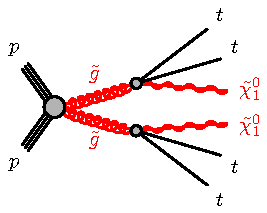
\includegraphics[width=0.24\textwidth]{MODELS/gogo-ttttN1N1}}
\subfigure{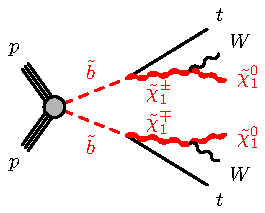
\includegraphics[width=0.24\textwidth]{MODELS/sbsb-ttWWN1N1}}
\caption{Gluino decay via offshell stop (left), and direct sbottom pair production (right).}
\label{fig:feynman_3rdgen}
\end{figure}

\begin{figure}[t]
\centering
\subfigure{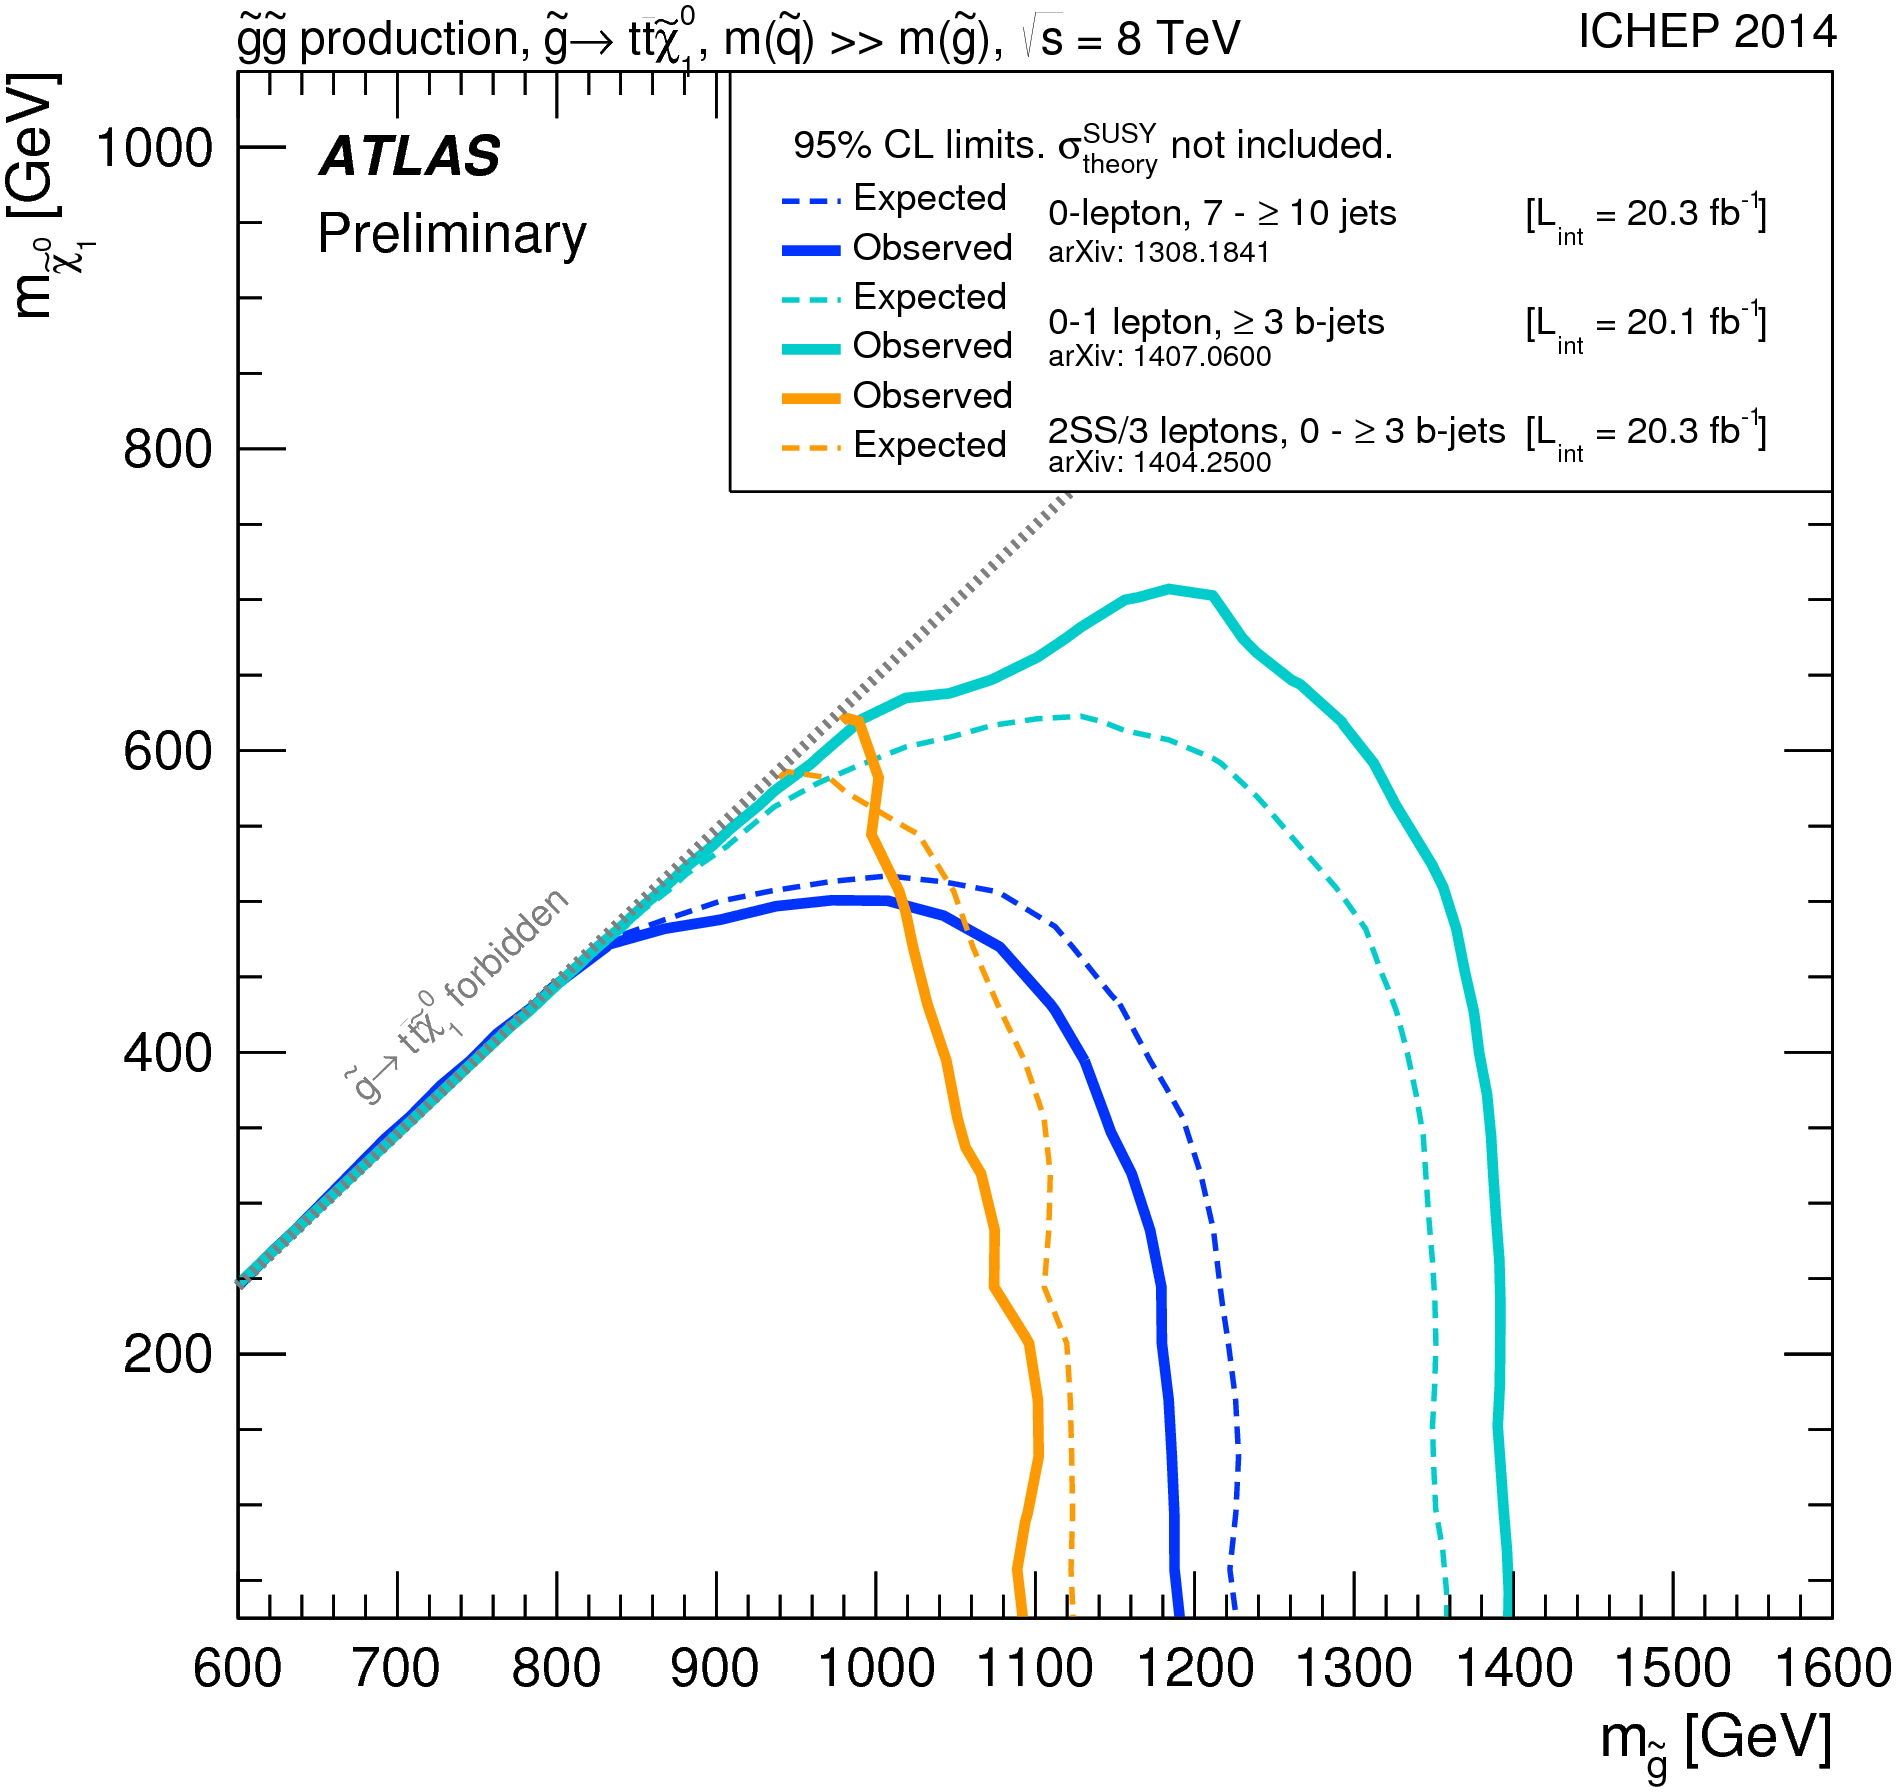
\includegraphics[width=0.49\textwidth]{MODELS/ATLAS_SUSY_Gtt}}
\subfigure{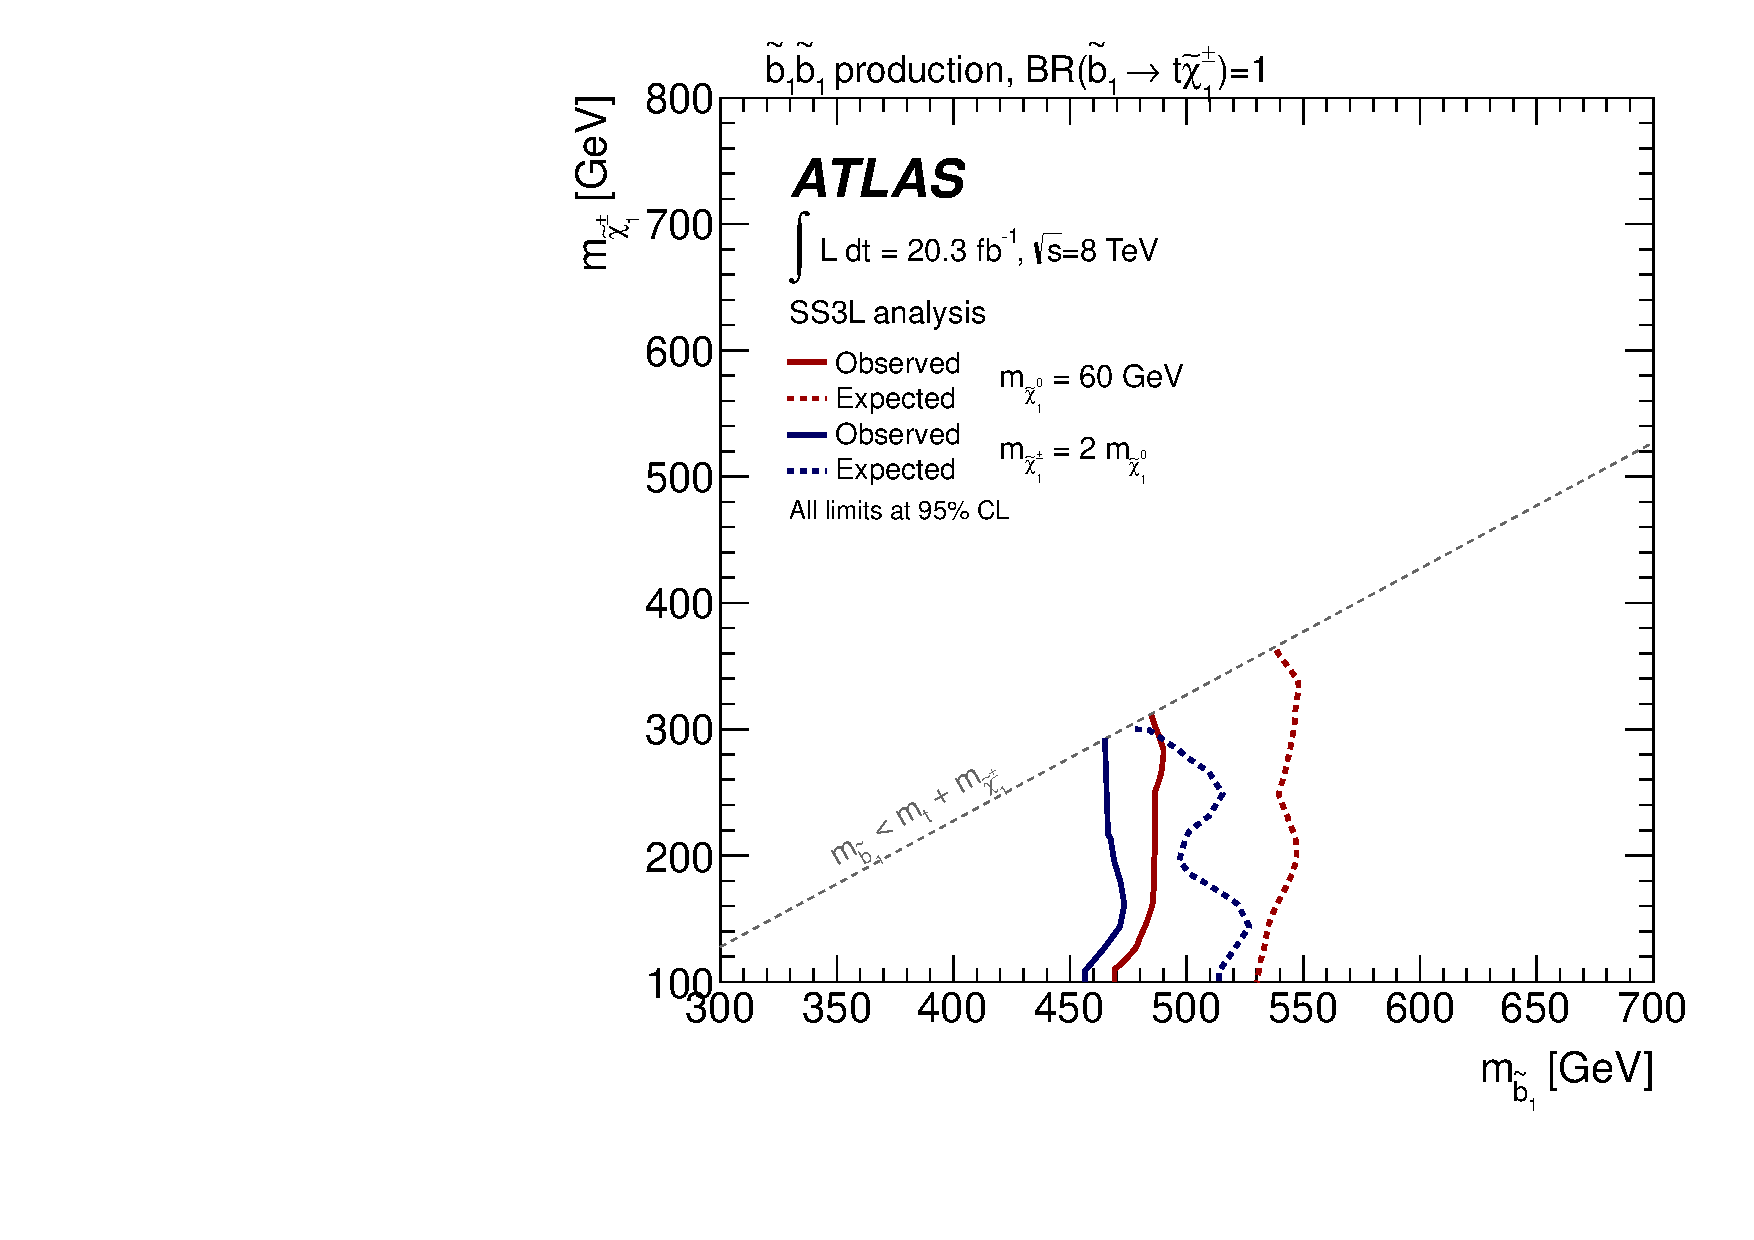
\includegraphics[width=0.49\textwidth]{MODELS/exclusion_sbottom_topC1_both_grids}}
\caption{Exclusion limits on the gluino-stop offshell (left) and direct sbottom (right) scenarios 
set by ATLAS with the 2012 dataset~\cite{DraftSquarkGluinoSummaryPaper}.}
\label{fig:run1excl_3rdgen}
\end{figure}

\par{\bf Gluino-stop offshell $\gluino\to t\bar t\neut$\\}
In this model inspired by naturalness arguments, gluinos are coupling preferentially to stops which are lighter than the other squarks. 
Gluinos are however considered lighter than stops, and decay directly into a $t\bar t\neut$ triplet via a virtual stop (Fig.~\ref{fig:feynman_3rdgen}). 
The pair production of gluinos leads to a final state containing four top quarks and two neutralinos. 
This characteristic final state is accessible through various experimental signatures, which is why this model 
is commonly used as a benchmark to estimate analyses sensitivities. 
The searches performed with run-1 data~\cite{DraftSquarkGluinoSummaryPaper}, 
summarized in Fig.~\ref{fig:run1excl_3rdgen}, showed that the same-sign leptons final state is competitive mainly at large neutralino mass. 
This region of the phase space is consequently given a particular attention in the choice of signal regions described further on. 
In the signal samples referenced in this document, the lightest stop mass is fixed to 10~\TeV and is mostly a $\widetilde{t}_R$ state. 
Only gluino pair production is considered, followed by an exclusive decay in the aforementioned channel. 
\\
\par{\bf Direct sbottom $\sbot\to t\chargino$\\}
In this model, bottom squarks are rather lights and assumed to decay in a top quark and a chargino $\chargino$ (Fig.~\ref{fig:feynman_3rdgen}), 
providing complementarity to the mainstream search which focuses on the channel $\sbot\to b\neut$. 
The final state resulting from the production of a sbottom pair contains pairs of top quarks, of $W$ bosons and of neutralinos. 
While this final state may lead to various experimental signatures, 
the model was considered in run-1~\cite{DraftSquarkGluinoSummaryPaper} 
only by the same-sign leptons and jets search, leading to the exclusion limits presented in Fig.~\ref{fig:run1excl_3rdgen}. 
In the signal samples used by the analysis, the neutralino mass is fixed to 60~\GeV, and the chargino mass to 150~\GeV, while the sbottom mass is varied. 
Only pair production of the lightest sbottom is considered, followed by an exclusive decay in the aforementioned channel. \\


\begin{figure}[h!]
\subfigure{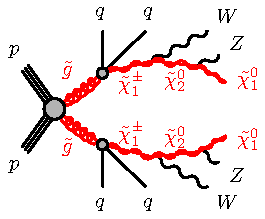
\includegraphics[width=0.24\textwidth]{MODELS/gogo-qqqqWWZZN1N1-C1N2}}
\subfigure{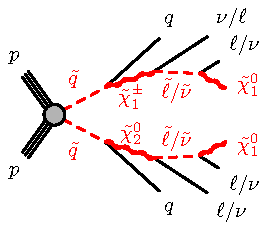
\includegraphics[width=0.24\textwidth]{MODELS/sqsq-qqlllvN1N1-C1N2}}
\subfigure{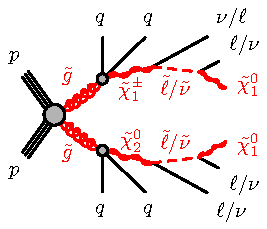
\includegraphics[width=0.24\textwidth]{MODELS/gogo-qqqqlllvN1N1-C1N2}}
\subfigure{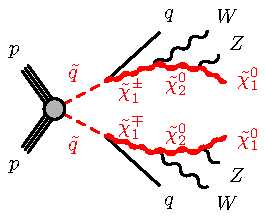
\includegraphics[width=0.24\textwidth]{MODELS/sqsq-qqWWZZN1N1-C1N2}}
\caption{Two-step decays of gluinos and squarks, mediated by gauginos (left) or sleptons (right).}
\label{fig:feynman_1stgen}
\end{figure}

\begin{figure}[t]
\centering
\subfigure{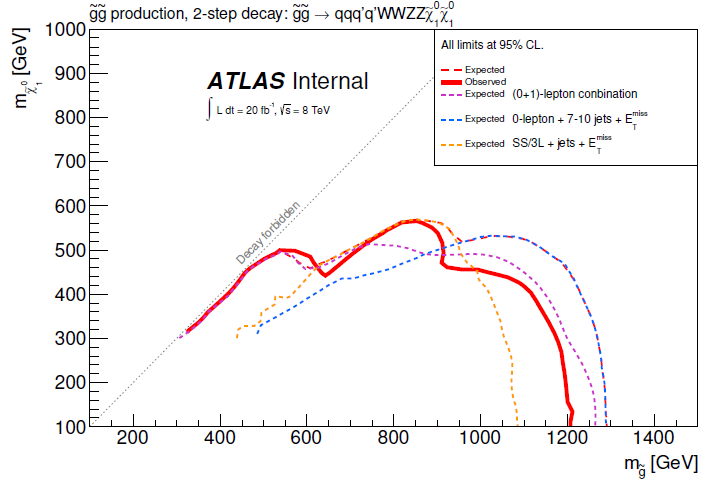
\includegraphics[width=0.49\textwidth]{MODELS/run1excluded_gluino2stepWZ}}
\subfigure{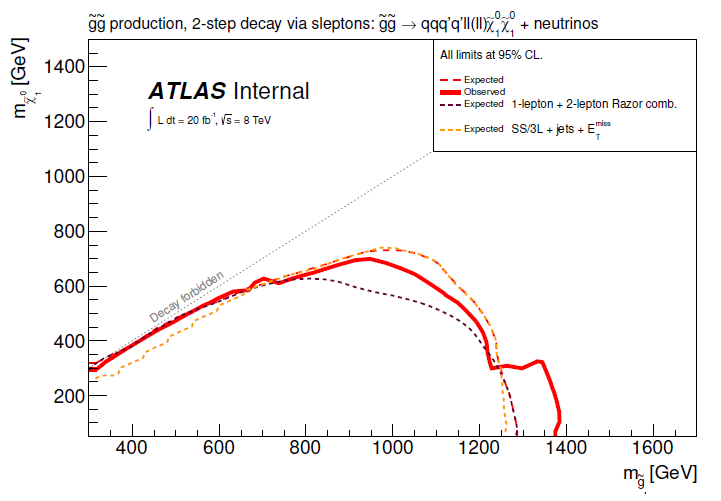
\includegraphics[width=0.49\textwidth]{MODELS/run1excluded_gluino2stepSleptons}}
\subfigure{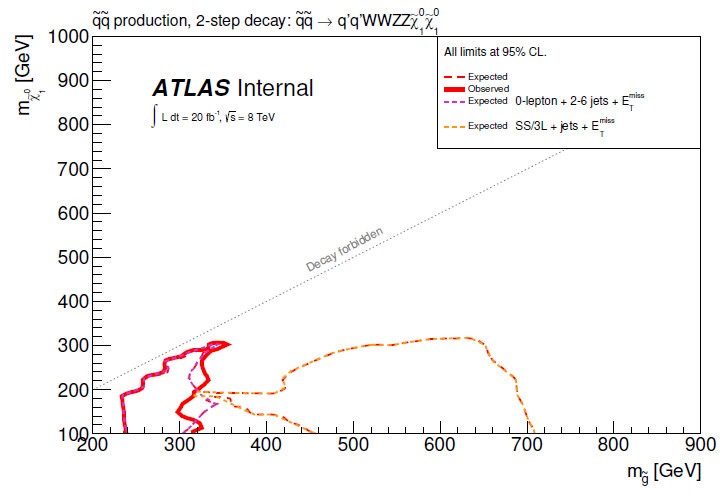
\includegraphics[width=0.49\textwidth]{MODELS/run1excluded_squark2stepWZ}}
\subfigure{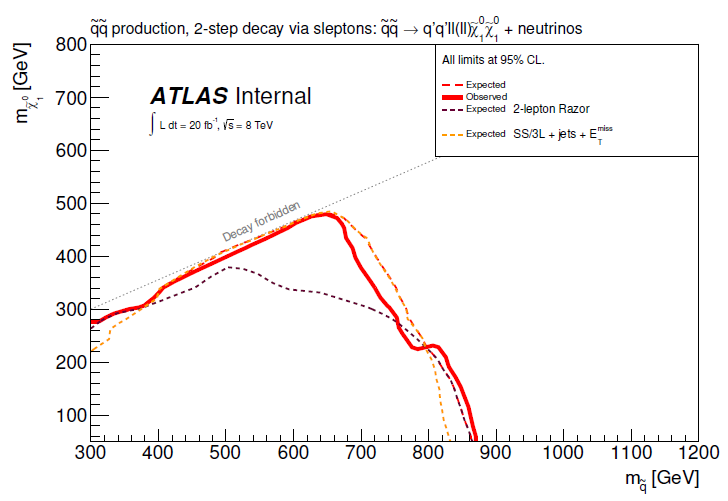
\includegraphics[width=0.49\textwidth]{MODELS/run1excluded_squark2stepSleptons}}
\caption{Exclusion limits on scenarios featuring gluino (top) and squarks (bottom) two-steps decays via gauginos (left) or sleptons (right) 
set by ATLAS with the 2012 dataset~\cite{DraftSquarkGluinoSummaryPaper}.}
\label{fig:run1excluded_1stgen}
\end{figure}

\par{\bf Gluinos and squarks 2-step decays via gauginos\\}
These scenarios feature a less oriented search for gluinos or squarks (save third generation) where gluinos couple preferentially to the latter, 
and squarks decay to charginos (Fig.~\ref{fig:feynman_1stgen} left) with the subsequent cascade $\chargino\to W\tilde{\chi}_{2}^{0} \to WZ\neut$. 
This leads to final states of two light quarks, two $W$ and $Z$ bosons, and two neutralinos 
(with two additional light quarks in the case of gluino pair production). 
Fig.~\ref{fig:run1excluded_1stgen} left shows the exclusion limits obtained with the 2012 dataset~\cite{DraftSquarkGluinoSummaryPaper}; 
in the gluino scenario, the same-sign leptons + jets search provided complementarity at large neutralino mass, 
while its sensitivity in the squark scenario dominated completely. 
In the signal samples used here, the chargino mass is set halfway between the neutralino and squark (or gluino) masses, 
while the neutralino $\tilde{\chi}_{2}^{0}$ mass is set halfway between the chargino and neutralino masses. 
Gluino and squark-antisquark pair production are considered separately in distinct scenarios.  
\\
\par{\bf Gluinos and squarks 2-step decays via sleptons\\}
In these scenarios, gluinos couple preferentially to the squarks of the first two generations, and
the latter decay either to a chargino $\chargino$ or a neutralino $\tilde{\chi}_{2}^{0}$, 
which are assumed to be mass-degenerate, and decay in turn to sleptons (Fig.~\ref{fig:feynman_1stgen} right) 
with $\mathcal{BR}(\chargino\to\nu\tilde\ell) = \mathcal{BR}(\chargino\to\ell\tilde\nu) 
= \mathcal{BR}(\tilde{\chi}_{2}^{0}\to\nu\tilde\nu) = \mathcal{BR}(\tilde{\chi}_{2}^{0}\to\ell\tilde\ell)=50\%$. 
The corresponding final state may contain zero to four charged leptons, neutrinos, two light quarks and two neutralinos 
(with two additional light quarks in the case of gluino pair production). 
Because of the sleptons replacing the gauge bosons featured in the scenarios presented in the previous paragraph, 
these scenarios have comparatively a lower jet multiplicity but a significantly enhanced acceptance in multi-lepton experimental signatures. 
As can be seen on Fig.~\ref{fig:run1excluded_1stgen} right, which presents the exclusion limits obtained with the 2012 dataset~\cite{DraftSquarkGluinoSummaryPaper}, 
the same-sign leptons and jets signature is again very competitive. 
In the signal samples used here, the chargino $\chargino$ and neutralino $\tilde{\chi}_{2}^{0}$ masses are set equal, 
halfway between the neutralino and squark (or gluino) masses, 
while the degenerate sleptons masses are set halfway between these gauginos and the lightest neutralino masses. 
Furthermore, gauginos decay to any slepton flavor with equal probability. 
Gluino and squark-antisquark pair production are considered separately in distinct scenarios. 
\\
\par{\bf Models not considered for the moment\\}
In the publications~\cite{paperSS3L,DraftSquarkGluinoSummaryPaper} of the analysis results obtained with run-1 data, 
exclusion limits were also provided for other signal models, often 
These scenarios included the $\gluino\to tbW\neut$ and $\gluino\to tcW\neut$ simplified models, as well as minimal models featuring 
$R$-parity violation through bilinear terms, gauge-mediated SUSY breaking, or universal extra dimensions. 
These models are not considered here, although interpretations might be proposed for them again in the future. 

\subsection{New models}

%\subsubsection{pMSSM inspired [Sebastien]}

\subsubsection{RPV inspired}
\label{subsec:RPVmodel}

 In supersymmetry, the following superpotential is present :
 \begin{align}
   W = \mu H L + \frac{1}{2} \lambda_{ijk} L_i L_j E_k + \lambda'_{ijk} L_i Q_j D_k + \frac{1}{2} \lambda''_{ijk} U_i D_j D_k
   \label{rpvpotential}
 \end{align}
 where $H$, $L$, $Q$, $E$, $U$ and $D$ are respectively the superpotential associated to the Higgs doublet, the lepton-neutrino doublet, the quark up-down doublet, the right-handed electron, the right-handed up quark and the right-handed down quark.
 The indices $i$, $j$ and $k$ are the flavor indices and $\mu$ , $\lambda_{ijk}$ , $\lambda'_{ijk}$ , $\lambda''_{ijk}$ are the coupling constants.
\\

 The leptonic number violation and the baryonic number violation implied by this potential have an important impact in the physic at low energy
 and do not respect some low energy constraints like the proton decay time limit.
 In $R$-parity conserving (RPC) SUSY models, the $R$-parity is added in order to remove these terms and keep the proton stable.
 However, one can play with the couplings $\mu$ , $\lambda_{ijk}$ , $\lambda'_{ijk}$ and $\lambda''_{ijk}$ in order to violate $R$-parity while respecting the low energy constraints.
 This is called the $R$-parity violation (RPV) SUSY models.
\\

 In this note, we will only consider the case where the coupling constants $\mu$, $\lambda_{ijk}$, $\lambda'_{ijk}$ and $\lambda''_{(i \neq 3) jk}$ are suppressed.
 Therefore, the only non-negligible terms are $\lambda''_{321}TSD$ , $\lambda''_{331}TBD$ and $\lambda''_{323}TSB$ where $T$, $B$, $D$ and $S$ are the superfields associated to the top, bottom, down and strange quark.
 This scenario is predicted by some RPV models like the Minimal Flavor Violation (MFV) scenarios~\cite{Nikolidakis:2007fc,Csaki:2011ge} and leads to the production of same-sign top quarks~\cite{Durieux:2013uqa} (see Fig.~\ref{fig:rpv_diagram}).

\begin{figure}[h!]
\centering
\subfigure{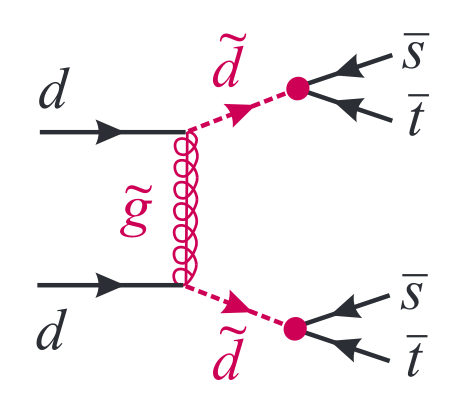
\includegraphics[width=0.24\textwidth]{MODELS/ddfusion.png}}
\subfigure{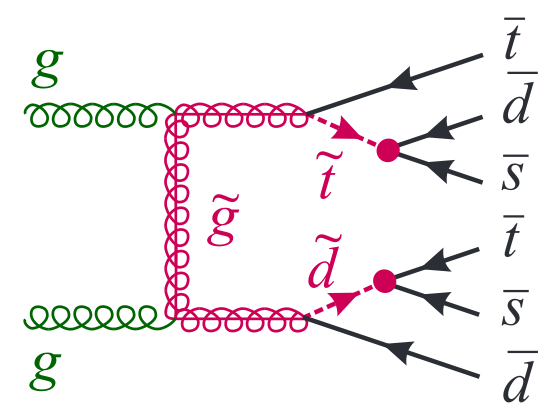
\includegraphics[width=0.27\textwidth]{MODELS/ggfusion.png}}
\caption{Example of diagrams for RPV model for the \textit{d-quark fusion} topology (left), and the \textit{gluon fusion} topology (right) involving the $\lambda''_{321}$ coupling. In both cases, the baryonic number is violated by two units. }
\label{fig:rpv_diagram}
\end{figure}

 In these scenarios, the $R$-parity is not conserved and the LSP is not stable (and therefore cannot be a good dark matter candidate).
 However, the interesting part of this model is that it allows B-violating processes (see Fig.~\ref{fig:rpv_diagram}).
 Actually, the baryonic asymmetry in the universe and the fact that the standard model does not respect this symmetry provides a good motivation for the search for $B$-violation processes at high energy.
 In addition, it was also proved that the violation of the baryonic number by two units involving top quarks could respect the low denergy constraints like the proton decay time limit~\cite{Durieux:2012gj}.
% Therefore, RPV SUSY is good generic model for the search for $B$-violation.
\\

In this analysis, two kind of topologies will be considered:
\begin{itemize}
\item \textbf{d-quark fusion}: Production of two on-shell $d$-squarks with a gluino in $t$-channel and the $d$-squarks decay to an anti-top quark and to one extra jet.
  The squarks will lighter than the gluino and the cross section will mostly depend on the mass of the squark (see Fig.~\ref{fig:rpv_diagram}).
  \begin{align}
    dd \to \tilde{d} \tilde{d}\ ,\ \tilde{d} \to \bar{t}q    
  \end{align}
\item \textbf{gluon fusion}: Production of two on-shell gluinos which decay to a top or an anti-top quark and to two extra jets.
  The gluino will be lighter than the squarks and the cross section will only depend on the mass of the gluino (see Fig.~\ref{fig:rpv_diagram} ).
  \begin{align}
    gg \to \gluino\gluino\ ,\ \gluino \to tqq\ /\ \gluino \to \bar{t}qq'
  \end{align}
\end{itemize}
The extra jets could be either $b$-jet or light jets, depending on the coupling being considered. 
In order to have access to the charge of the top quark, we will only consider the case where the top quark decays leptonically.
At the end, the final states will be composed of two same-sign leptons, at least two $b$-jets, low missing transverse energy (coming from the neutrinos) and extra jets.
\\
% Cross section : soon

 This model was already constrained by ATLAS~\cite{Aad:2014pda} and CMS~\cite{Chatrchyan:2013fea} in Run-1, but those analyses 
 only considered the coupling $\lambda''_{323}$ and the topology of \textit{gluon fusion}.
 A limit of around 900 GeV was found on the mass of the gluino. The full hadronic final state was also exploited in ATLAS~\cite{Aad:2013wta}.



\section{MC samples}
\label{sec:samples}
This section summarizes the signal and background samples used for the
studies presented in this note, as well some details about the Monte Carlo production and analysis framework.
All samples used in this note are part of the DC14 Monte-Carlo campaign which exhibits a number 
of deficiencies~\cite{dc14twiki}, most notably the inaccessibility of detailed trigger information. 

\subsection{Derivation versions and analysis model}
\label{sec:ntuples}

In all cases, the SUSY1 DxAOD derivations are used. 
Derivation tag p1872 (19.1.4.9 cache) is used for most of the samples used in this note, although some signal 
samples were not initially available in that tag and p1863 (19.1.4.8 cache) was used instead. 
Both derivation tags included the fix of lepton isolation 
variables (see Section~\ref{sec:isolation} for more details).

Most of the studies shown in this note were performed using flat ROOT ntuples produced on the grid using code based on the 
{\tt{SUSYAnalysiExample}} EventLoop package and SUSYTools-00-05-00-26 tag. 
They contained basic object information, although no overlap removal 
or isolation cuts were applied to allow flexibility for optimization studies. 
No event skimming or systematic uncertainties were included. 
The total size of these ntuples is 70~GB (both background and signal samples).
These files were shared among the groups participating in the analysis, although some 
of the groups developed their own framework for xAOD analysis.

In addition, dedicated flat ROOT ntuples with all the systematic variations included in the SUSYTools {\tt getSystInfoList()} method 
were also produced for the samples containing prompt SS/3L ($\ttbar+V$, $\ttbar+h$, diboson, signals). To reduce the size of the output files, only events that contained in any of the systematic variations
at least 2 leptons with $\pt>10$~GeV, and either $\et>100$~GeV or at least 3 b-tagged jets ($\pT>20$ GeV) or $H_{\rm T}>300$~GeV were kept.  
In order to benefit from the recently implemented grouping of 
the Egamma systematics, the SUSYTools-00-05-00-29 tag was used for this production, which contains only other minor 
updates with respect to SUSYTools-00-05-00-26. The total size of these ntuples is below 50~GB.


\subsection{Signal Samples}

This section describes the signal samples used for in this note. 
The baseline signal models used are the ones described
in Section~\ref{sec:signal}, and all the signal samples used are listed in Table~\ref{tab:SignalSamples}.

The gluino-stop offshell ($\gluino\to t\bar t\neut$) and direct sbottom ($\sbot\to t\chargino$ with $\tilde{b}_1\to t\tilde{\chi}^{\pm}_1$) samples are produced with {\sc Herwig++}~\cite{Corcella:2000bw}. The UE-EE-4 {\sc Herwig++} tune~\cite{Gieseke:2012ft} is used to describe the underlying event.
%and the generator settings are equivalent to those of the 8 TeV 
%analysis~\cite{noteSS3L} except that the stop mass has been raised to 5
%TeV and the center of mass energy has been adjusted to 13 TeV.
The other signal samples used in this note (gluinos and squarks 2-step decays via gauginos or sleptons) are produced using the {\sc Madgraph v5} generator~\cite{madgraph} using leading-order (LO) matrix elements with up to two additional partons.
{\sc Pythia} 6.425~\cite{Sjostrand:2006za} with the {\sc AUET2B} tune~\cite{pub-2011-009,ATLAS:2011krm} is used for hadronisation and to describe the underlying event. 
In all the signal samples, the {\sc CTEQ6L1}~\cite{Pumplin:2002vw} set of parton distribution functions is used in all the signal samples. The signal samples are normalised to the next-to-next-to-leading order cross-section including the resummation of
soft gluon emission at next-to-next-to-leading-logarithmic accuracy
(NLO+NLL), as detailed in Ref.~\cite{Borschensky:2014cia}. 


\begin{sidewaystable}[htb]
\begin{center}
\resizebox{0.95\textwidth}{!}{
\tiny
\begin{tabular}{lllllll}
\hline
\hline
datasetID & Sample name & $\sigma$ [pb] & $k$-Factor & $\epsilon_{filter}$ & $N_{gen}$ & $L_{equiv}$\\
\hline
\multicolumn{7}{c}{\textbf{Gluino-stop offshell} ($\gluino\to t\bar t\neut$)} \\ \hline
204533  &  mc14\_13TeV.204533.Herwigpp\_UEEE4\_CTEQ6L1\_Gtt\_G1000\_T5000\_L100.merge.DAOD\_SUSY1.e3094\_s1982\_s2008\_r5787\_r5853\_p1872/  &  0.3254  &  1.00  &  1.000  &  20000  &  61.5 \\
204534  &  mc14\_13TeV.204534.Herwigpp\_UEEE4\_CTEQ6L1\_Gtt\_G1300\_T5000\_L100.merge.DAOD\_SUSY1.e3094\_s1982\_s2008\_r5787\_r5853\_p1872/  &  0.0461  &  1.00  &  1.000  &  19500  &  423.0 \\
204535  &  mc14\_13TeV.204535.Herwigpp\_UEEE4\_CTEQ6L1\_Gtt\_G1600\_T5000\_L100.merge.DAOD\_SUSY1.e3094\_s1982\_s2008\_r5787\_r5853\_p1872/  &  0.0081  &  1.00  &  1.000  &  20000  &  2469.1 \\
204536  &  mc14\_13TeV.204536.Herwigpp\_UEEE4\_CTEQ6L1\_Gtt\_G1900\_T5000\_L100.merge.DAOD\_SUSY1.e3094\_s1982\_s2008\_r5787\_r5853\_p1872/  &  0.0016  &  1.00  &  1.000  &  20000  &  12500.0 \\
204537  &  mc14\_13TeV.204537.Herwigpp\_UEEE4\_CTEQ6L1\_Gtt\_G2200\_T5000\_L100.merge.DAOD\_SUSY1.e3094\_s1982\_s2008\_r5787\_r5853\_p1872/  &  0.0004  &  1.00  &  1.000  &  20000  &  50000.0 \\
204539  &  mc14\_13TeV.204539.Herwigpp\_UEEE4\_CTEQ6L1\_Gtt\_G1300\_T5000\_L400.merge.DAOD\_SUSY1.e3094\_s1982\_s2008\_r5787\_r5853\_p1872/  &  0.0461  &  1.00  &  1.000  &  15000  &  325.4 \\
204540  &  mc14\_13TeV.204540.Herwigpp\_UEEE4\_CTEQ6L1\_Gtt\_G1300\_T5000\_L700.merge.DAOD\_SUSY1.e3094\_s1982\_s2008\_r5787\_r5853\_p1872/  &  0.0461  &  1.00  &  1.000  &  20000  &  433.8 \\
204541  &  mc14\_13TeV.204541.Herwigpp\_UEEE4\_CTEQ6L1\_Gtt\_G1300\_T5000\_L900.merge.DAOD\_SUSY1.e3094\_s1982\_s2008\_r5787\_r5853\_p1872/  &  0.0461  &  1.00  &  1.000  &  20000  &  433.8 \\
204912  &  mc14\_13TeV.204912.Herwigpp\_UEEE4\_CTEQ6L1\_Gtt\_G1500\_T5000\_L200.merge.DAOD\_SUSY1.e3328\_s1982\_s2008\_r5787\_r5853\_p1872/  &  0.0142  &  1.00  &  1.000  &  20000  &  1408.5 \\
204913  &  mc14\_13TeV.204913.Herwigpp\_UEEE4\_CTEQ6L1\_Gtt\_G1500\_T5000\_L400.merge.DAOD\_SUSY1.e3328\_s1982\_s2008\_r5787\_r5853\_p1872/  &  0.0142  &  1.00  &  1.000  &  20000  &  1408.5 \\
204914  &  mc14\_13TeV.204914.Herwigpp\_UEEE4\_CTEQ6L1\_Gtt\_G1500\_T5000\_L600.merge.DAOD\_SUSY1.e3328\_s1982\_s2008\_r5787\_r5853\_p1872/  &  0.0142  &  1.00  &  1.000  &  20000  &  1408.5 \\
204915  &  mc14\_13TeV.204915.Herwigpp\_UEEE4\_CTEQ6L1\_Gtt\_G1500\_T5000\_L800.merge.DAOD\_SUSY1.e3328\_s1982\_s2008\_r5787\_r5853\_p1872/  &  0.0142  &  1.00  &  1.000  &  20000  &  1408.5 \\
204916  &  mc14\_13TeV.204916.Herwigpp\_UEEE4\_CTEQ6L1\_Gtt\_G1500\_T5000\_L1000.merge.DAOD\_SUSY1.e3328\_s1982\_s2008\_r5787\_r5853\_p1872/  &  0.0142  &  1.00  &  1.000  &  20000  &  1408.5 \\ \hline
\multicolumn{7}{c}{\textbf{Direct sbottom} ($\sbot\to t\chargino$ with $\tilde{b}_1\to t\tilde{\chi}^{\pm}_1$)} \\ \hline
204973  &  mc14\_13TeV.204973.Herwigpp\_UEEE4\_CTEQ6L1\_sbottom\_tchr\_2lep\_B450\_C150\_N60.merge.DAOD\_SUSY1.e3356\_s1982\_s2008\_r5787\_r5853\_p1863/  &  0.9483  &  0.41  &  0.409  &  20000  &  125.8 \\
204974  &  mc14\_13TeV.204974.Herwigpp\_UEEE4\_CTEQ6L1\_sbottom\_tchr\_2lep\_B550\_C150\_N60.merge.DAOD\_SUSY1.e3356\_s1982\_s2008\_r5787\_r5853\_p1863/  &  0.2961  &  0.43  &  0.432  &  11000  &  200.0 \\
204975  &  mc14\_13TeV.204975.Herwigpp\_UEEE4\_CTEQ6L1\_sbottom\_tchr\_2lep\_B650\_C150\_N60.merge.DAOD\_SUSY1.e3356\_s1982\_s2008\_r5787\_r5853\_p1863/  &  0.1070  &  0.45  &  0.451  &  20000  &  921.0 \\
204976  &  mc14\_13TeV.204976.Herwigpp\_UEEE4\_CTEQ6L1\_sbottom\_tchr\_2lep\_B750\_C150\_N60.merge.DAOD\_SUSY1.e3356\_s1982\_s2008\_r5787\_r5853\_p1863/  &  0.0431  &  0.47  &  0.472  &  20000  &  2091.8 \\
204977  &  mc14\_13TeV.204977.Herwigpp\_UEEE4\_CTEQ6L1\_sbottom\_tchr\_2lep\_B850\_C150\_N60.merge.DAOD\_SUSY1.e3356\_s1982\_s2008\_r5787\_r5853\_p1863/  &  0.0190  &  0.48  &  0.483  &  20000  &  4540.3 \\
\hline
\multicolumn{7}{c}{\textbf{gluino 2-step decays via gauginos}} \\ \hline
204952  &  mc14\_13TeV.204952.MadGraphPythia\_AUET2BCTEQ6L1\_SMGG2WWZZ\_1100\_600\_100.merge.DAOD\_SUSY1.e3345\_s1982\_s2008\_r5787\_r5853\_p1872/  &  0.1635  &  1.00  &  1.000  &  19500  &  119.3 \\
204953  &  mc14\_13TeV.204953.MadGraphPythia\_AUET2BCTEQ6L1\_SMGG2WWZZ\_1300\_700\_100.merge.DAOD\_SUSY1.e3345\_s1982\_s2008\_r5787\_r5853\_p1872/  &  0.0461  &  1.00  &  1.000  &  5000  &  108.5 \\
204954  &  mc14\_13TeV.204954.MadGraphPythia\_AUET2BCTEQ6L1\_SMGG2WWZZ\_1500\_800\_100.merge.DAOD\_SUSY1.e3345\_s1982\_s2008\_r5787\_r5853\_p1872/  &  0.0142  &  1.00  &  1.000  &  20000  &  1408.5 \\
204955  &  mc14\_13TeV.204955.MadGraphPythia\_AUET2BCTEQ6L1\_SMGG2WWZZ\_1700\_900\_100.merge.DAOD\_SUSY1.e3345\_s1982\_s2008\_r5787\_r5853\_p1872/  &  0.0047  &  1.00  &  1.000  &  15000  &  3191.5 \\
204956  &  mc14\_13TeV.204956.MadGraphPythia\_AUET2BCTEQ6L1\_SMGG2WWZZ\_1900\_1000\_100.merge.DAOD\_SUSY1.e3345\_s1982\_s2008\_r5787\_r5853\_p1872/  &  0.0016  &  1.00  &  1.000  &  15500  &  9687.5 \\
204957  &  mc14\_13TeV.204957.MadGraphPythia\_AUET2BCTEQ6L1\_SMGG2WWZZ\_2100\_1100\_100.merge.DAOD\_SUSY1.e3345\_s1982\_s2008\_r5787\_r5853\_p1872/  &  0.0006  &  1.00  &  1.000  &  5000  &  8333.3 \\
204958  &  mc14\_13TeV.204958.MadGraphPythia\_AUET2BCTEQ6L1\_SMGG2WWZZ\_2300\_1200\_100.merge.DAOD\_SUSY1.e3345\_s1982\_s2008\_r5787\_r5853\_p1872/  &  0.0002  &  1.00  &  1.000  &  13500  &  67500.0 \\
204959  &  mc14\_13TeV.204959.MadGraphPythia\_AUET2BCTEQ6L1\_SMGG2WWZZ\_1000\_700\_400.merge.DAOD\_SUSY1.e3345\_s1982\_s2008\_r5787\_r5853\_p1872/  &  0.3254  &  1.00  &  1.000  &  5000  &  15.4 \\
204960  &  mc14\_13TeV.204960.MadGraphPythia\_AUET2BCTEQ6L1\_SMGG2WWZZ\_1000\_750\_500.merge.DAOD\_SUSY1.e3345\_s1982\_s2008\_r5787\_r5853\_p1872/  &  0.3254  &  1.00  &  1.000  &  7500  &  23.0 \\
204961  &  mc14\_13TeV.204961.MadGraphPythia\_AUET2BCTEQ6L1\_SMGG2WWZZ\_1000\_800\_600.merge.DAOD\_SUSY1.e3345\_s1982\_s2008\_r5787\_r5853\_p1872/  &  0.3254  &  1.00  &  1.000  &  20000  &  61.5 \\
204962  &  mc14\_13TeV.204962.MadGraphPythia\_AUET2BCTEQ6L1\_SMGG2WWZZ\_1000\_850\_700.merge.DAOD\_SUSY1.e3345\_s1982\_s2008\_r5787\_r5853\_p1872/  &  0.3254  &  1.00  &  1.000  &  20000  &  61.5 \\
204963  &  mc14\_13TeV.204963.MadGraphPythia\_AUET2BCTEQ6L1\_SMGG2WWZZ\_1000\_900\_800.merge.DAOD\_SUSY1.e3345\_s1982\_s2008\_r5787\_r5853\_p1872/  &  0.3254  &  1.00  &  1.000  &  20000  &  61.5 \\
204964  &  mc14\_13TeV.204964.MadGraphPythia\_AUET2BCTEQ6L1\_SMGG2WWZZ\_1000\_950\_900.merge.DAOD\_SUSY1.e3345\_s1982\_s2008\_r5787\_r5853\_p1872/  &  0.3254  &  1.00  &  1.000  &  10000  &  30.7 \\
\hline
\multicolumn{7}{c}{\textbf{squark 2-step decays via gauginos}} \\ \hline
204965  &  mc14\_13TeV.204965.MadGraphPythia\_AUET2BCTEQ6L1\_SMSS2WWZZ\_650\_375\_100.merge.DAOD\_SUSY1.e3345\_s1982\_s2008\_r5787\_r5853\_p1872/  &  0.0695  &  1.00  &  1.000  &  5000  &  71.9 \\
204966  &  mc14\_13TeV.204966.MadGraphPythia\_AUET2BCTEQ6L1\_SMSS2WWZZ\_750\_425\_100.merge.DAOD\_SUSY1.e3345\_s1982\_s2008\_r5787\_r5853\_p1872/  &  0.0219  &  1.00  &  1.000  &  20000  &  913.2 \\
204967  &  mc14\_13TeV.204967.MadGraphPythia\_AUET2BCTEQ6L1\_SMSS2WWZZ\_850\_475\_100.merge.DAOD\_SUSY1.e3345\_s1982\_s2008\_r5787\_r5853\_p1872/  &  0.0075  &  1.00  &  1.000  &  17500  &  2333.3 \\
204968  &  mc14\_13TeV.204968.MadGraphPythia\_AUET2BCTEQ6L1\_SMSS2WWZZ\_950\_525\_100.merge.DAOD\_SUSY1.e3345\_s1982\_s2008\_r5787\_r5853\_p1872/  &  0.0027  &  1.00  &  1.000  &  19000  &  7037.0 \\
204969  &  mc14\_13TeV.204969.MadGraphPythia\_AUET2BCTEQ6L1\_SMSS2WWZZ\_650\_475\_300.merge.DAOD\_SUSY1.e3345\_s1982\_s2008\_r5787\_r5853\_p1872/  &  0.0695  &  1.00  &  1.000  &  20000  &  287.8 \\
204970  &  mc14\_13TeV.204970.MadGraphPythia\_AUET2BCTEQ6L1\_SMSS2WWZZ\_650\_525\_400.merge.DAOD\_SUSY1.e3345\_s1982\_s2008\_r5787\_r5853\_p1872/  &  0.0695  &  1.00  &  1.000  &  20000  &  287.8 \\
204971  &  mc14\_13TeV.204971.MadGraphPythia\_AUET2BCTEQ6L1\_SMSS2WWZZ\_650\_575\_500.merge.DAOD\_SUSY1.e3345\_s1982\_s2008\_r5787\_r5853\_p1872/  &  0.0695  &  1.00  &  1.000  &  20000  &  287.8 \\
204972  &  mc14\_13TeV.204972.MadGraphPythia\_AUET2BCTEQ6L1\_SMSS2WWZZ\_650\_625\_600.merge.DAOD\_SUSY1.e3345\_s1982\_s2008\_r5787\_r5853\_p1872/  &  0.0695  &  1.00  &  1.000  &  20000  &  287.8 \\
\hline
\hline
\end{tabular}}
\end{center}
\caption{List of simulated samples for the signal models used in this note. The dataset ID, the 
  cross-section $\sigma$, the $k$-Factor, the generator filter
  efficiency $\epsilon_{filter}$, the total number of
  generated events $N_{gen}$ and the equivalent luminosity ($L_{equiv}$) are shown.}
\label{tab:SignalSamples}
\end{sidewaystable}



\subsection{Background Samples}
\label{sec:BGSamples}

All the background samples used are listed in Tables~\ref{tab:BGSamples1}-\ref{tab:BGSamples3}.

Simulated $t\bar{t}$ events are generated using the {\sc Powheg} generator
version r2330.2 ~\cite{Nason:2004rx,Frixione:2007vw,Alioli:2010xd}, which implements
the next-to-leading order matrix element for inclusive $t\bar{t}$
production and uses the
CT10 PDF set~\cite{Lai:2010vv}. {\sc Powheg} is interfaced to {\sc Pythia} 6.427~\cite{Sjostrand:2006za}
with the CTEQ6L1 PDF set using the
Perugia2012 tune~\cite{Skands:2010ak}. The $t\bar{t}$ samples are normalised to their
next-to-next-to-leading order cross-section including the resummation of
soft gluon emission at next-to-next-to-leading-logarithmic accuracy
using Top++2.0 ~\cite{Czakon:2011xx}.

Simulated $W$/$Z$+jets samples are produced using {\sc Sherpa} 1.4.5
~\cite{gleisberg:2008ta} with massive $b$-, $c$-quarks with up to four
additional partons in the matrix element and parton shower and are
normalised to their next-to-next-to-leading order QCD theoretical
cross sections~\cite{Catani:2009sm}.

Samples of single top quark backgrounds corresponding to the $t$-, $s$-
and $Wt$ production mechanisms are generated with {\sc Powheg} version r2330.2
using the CT10 PDF set. All single-top samples are interfaced to {\sc Pythia} 6.427
with the CTEQ6L1 set of parton distribution functions using the
Perugia2012 tune. The leading-order cross-sections obtained from the
generator is used for these samples.

The processes of $t\bar{t}+V$ production are generated with {\sc MadGraph} 5
2.1.1~\cite{madgraph} + {\sc Pythia} 6.427 using the CTEQ6L1 set of parton
distribution functions and the AUET2B underlying event
tune~\cite{ATLAS:2011krm}. The samples are normalised to their
next-to-leading order cross-sections using the $k$-factors computed for $\sqrt{s}=14$~TeV~\cite{Campbell:2012dh,Kardos:2011na}. 

% 
Simulated samples for diboson processes are simulated with {\sc Sherpa} 1.4.5 ($WZ/ZZ\to\ell\ell\nu\nu$ and $W^{\pm}W^{\pm}jj\to\ell^{\pm}\ell^{\pm}\nu\nu jj$ electroweak production), {\sc Powheg} r2330.3 + {\sc Pythia 8} ($WW$, $WZ$ and $ZZ$) and {\tt gg2VV}~\cite{Kauer:2013qba,Kauer:2012hd} in {\sc Powheg} r2330.3 + {\sc Pythia 8} ($gg\to h\to WW$).

QCD multijets are not included in this study since these
backgrounds are expected to be very small.
Note that some background processes that had a non-negligible (despite small) contribution to the analysis in Run-1,
such as tri-boson or $t+Z$ production, were not included in the DC14 productions.

% Processes involving Higgs production are generated with PYTHIA8.
\begin{sidewaystable}[h]
\begin{center}
\resizebox{0.9\textwidth}{!}{
\tiny
\begin{tabular}{lllllll}
\hline
\hline
datasetID & Sample name & $\sigma$ [pb] & $k$-Factor & $\epsilon_{filter}$ & $N_{gen}$ & $L_{equiv}$\\
\hline
110401  &  mc14\_13TeV.110401.PowhegPythia\_P2012\_ttbar\_nonallhad.merge.DAOD\_SUSY1.e2928\_s1982\_s2008\_r5787\_r5853\_p1872/  &  831.7600  &  1.00  &  0.543  &  9970500  &  22.1 \\
119353  &  mc14\_13TeV.119353.MadGraphPythia\_AUET2BCTEQ6L1\_ttbarW.merge.DAOD\_SUSY1.e3214\_s1982\_s2008\_r5787\_r5853\_p1872/  &  0.2014  &  1.22  &  1.000  &  399500  &  1625.9 \\
119355  &  mc14\_13TeV.119355.MadGraphPythia\_AUET2BCTEQ6L1\_ttbarZ.merge.DAOD\_SUSY1.e3214\_s1982\_s2008\_r5787\_r5853\_p1872/  &  0.1857  &  1.56  &  1.000  &  400000  &  1380.8 \\
119583  &  mc14\_13TeV.119583.MadgraphPythia\_AUET2B\_CTEQ6L1\_ttbarWW.merge.DAOD\_SUSY1.e3214\_s1982\_s2008\_r5787\_r5853\_p1872/  &  0.0030  &  1.00  &  1.000  &  10000  &  3333.3 \\
174830  &  mc14\_13TeV.174830.MadGraphPythia\_AUET2BCTEQ6L1\_ttbarWjExcl.merge.DAOD\_SUSY1.e3214\_s1982\_s2008\_r5787\_r5853\_p1872/  &  0.1313  &  1.22  &  1.000  &  399500  &  2494.0 \\
174831  &  mc14\_13TeV.174831.MadGraphPythia\_AUET2BCTEQ6L1\_ttbarWjjIncl.merge.DAOD\_SUSY1.e3214\_s1982\_s2008\_r5787\_r5853\_p1872/  &  0.1627  &  1.22  &  1.000  &  395000  &  1990.0 \\
174832  &  mc14\_13TeV.174832.MadGraphPythia\_AUET2BCTEQ6L1\_ttbarZjExcl.merge.DAOD\_SUSY1.e3214\_s1982\_s2008\_r5787\_r5853\_p1872/  &  0.1663  &  1.56  &  1.000  &  399500  &  1539.9 \\
174833  &  mc14\_13TeV.174833.MadGraphPythia\_AUET2BCTEQ6L1\_ttbarZjjIncl.merge.DAOD\_SUSY1.e3214\_s1982\_s2008\_r5787\_r5853\_p1872/  &  0.2076  &  1.56  &  1.000  &  399500  &  1233.6 \\
110070  &  mc14\_13TeV.110070.PowhegPythia\_P2012\_singletop\_tchan\_lept\_top.merge.DAOD\_SUSY1.e3049\_s1982\_s2008\_r5787\_r5853\_p1872/  &  43.7550  &  1.00  &  1.000  &  999000  &  22.8 \\

110071  &  mc14\_13TeV.110071.PowhegPythia\_P2012\_singletop\_tchan\_lept\_antitop.merge.DAOD\_SUSY1.e3049\_s1982\_s2008\_r5787\_r5853\_p1872/  &  25.7780  &  1.00  &  1.000  &  1000000  &  38.8 \\

110302  &  mc14\_13TeV.110302.PowhegPythia\_P2012\_st\_schan\_lep.merge.DAOD\_SUSY1.e3049\_s1982\_s2008\_r5787\_r5853\_p1872/  &  3.3514  &  1.00  &  1.000  &  999500  &  298.2 \\

110305  &  mc14\_13TeV.110305.PowhegPythia\_P2012\_st\_Wtchan\_incl\_DR.merge.DAOD\_SUSY1.e3049\_s1982\_s2008\_r5787\_r5853\_p1872/  &  68.4590  &  1.00  &  1.000  &  958500  &  14.0 \\
%\hline
%161105 & mc14\_13TeV.161105.Pythia8\_AU2CTEQ6L1\_WH125\_WW2lep.merge.DAOD\_SUSY1.e2743\_s1982\_s2008\_r5787\_r5853\_p1872/ & 0.24 & 1.00 & 0.104 & 0.025 & 100000  \\ 
%161155 & mc14\_13TeV.161155.Pythia8\_AU2CTEQ6L1\_ZH125\_WW2lep.merge.DAOD\_SUSY1.e2743\_s1982\_s2008\_r5787\_r5853\_p1872/ & 0.01 & 1.00 & 1.000 & 0.014 & 100000  \\ 
%161305 & mc14\_13TeV.161305.Pythia8\_AU2CTEQ6L1\_ttH125\_WWinclusive.merge.DAOD\_SUSY1.e2743\_s1982\_s2008\_r5787\_r5853\_p1872/ & 0.07 & 1.00 & 1.000 & 0.071 & 199500  \\ 
\hline
167740  &  mc14\_13TeV.167740.Sherpa\_CT10\_WenuMassiveCBPt0\_BFilter.merge.DAOD\_SUSY1.e2822\_s1982\_s2008\_r5787\_r5853\_p1872/  &  18795.0000  &  1.07  &  0.018  &  497000  &  1.4 \\
167741  &  mc14\_13TeV.167741.Sherpa\_CT10\_WenuMassiveCBPt0\_CJetFilterBVeto.merge.DAOD\_SUSY1.e2822\_s1982\_s2008\_r5787\_r5853\_p1872/  &  18804.0000  &  1.07  &  0.063  &  494500  &  0.4 \\
167742  &  mc14\_13TeV.167742.Sherpa\_CT10\_WenuMassiveCBPt0\_CJetVetoBVeto.merge.DAOD\_SUSY1.e2822\_s1982\_s2008\_r5787\_r5853\_p1872/  &  18843.0000  &  1.07  &  0.919  &  1000000  &  0.1 \\
167743  &  mc14\_13TeV.167743.Sherpa\_CT10\_WmunuMassiveCBPt0\_BFilter.merge.DAOD\_SUSY1.e2822\_s1982\_s2008\_r5787\_r5853\_p1872/  &  18793.0000  &  1.07  &  0.018  &  499500  &  1.4 \\
167744  &  mc14\_13TeV.167744.Sherpa\_CT10\_WmunuMassiveCBPt0\_CJetFilterBVeto.merge.DAOD\_SUSY1.e2822\_s1982\_s2008\_r5787\_r5853\_p1872/  &  18788.0000  &  1.07  &  0.056  &  498000  &  0.4 \\
167745  &  mc14\_13TeV.167745.Sherpa\_CT10\_WmunuMassiveCBPt0\_CJetVetoBVeto.merge.DAOD\_SUSY1.e2822\_s1982\_s2008\_r5787\_r5853\_p1872/  &  18797.0000  &  1.07  &  0.926  &  989500  &  0.1 \\
167746  &  mc14\_13TeV.167746.Sherpa\_CT10\_WtaunuMassiveCBPt0\_BFilter.merge.DAOD\_SUSY1.e2822\_s1982\_s2008\_r5787\_r5853\_p1872/  &  18795.0000  &  1.07  &  0.018  &  500000  &  1.4 \\
167747  &  mc14\_13TeV.167747.Sherpa\_CT10\_WtaunuMassiveCBPt0\_CJetFilterBVeto.merge.DAOD\_SUSY1.e2822\_s1982\_s2008\_r5787\_r5853\_p1872/  &  18808.0000  &  1.07  &  0.060  &  500000  &  0.4 \\
167748  &  mc14\_13TeV.167748.Sherpa\_CT10\_WtaunuMassiveCBPt0\_CJetVetoBVeto.merge.DAOD\_SUSY1.e2822\_s1982\_s2008\_r5787\_r5853\_p1872/  &  18800.0000  &  1.07  &  0.923  &  499500  &  0.0 \\
167761  &  mc14\_13TeV.167761.Sherpa\_CT10\_WenuMassiveCBPt70\_140\_BFilter.merge.DAOD\_SUSY1.e2822\_s1982\_s2008\_r5787\_r5853\_p1872/  &  557.8700  &  1.07  &  0.055  &  349500  &  10.6 \\
167762  &  mc14\_13TeV.167762.Sherpa\_CT10\_WenuMassiveCBPt70\_140\_CJetFilterBVeto.merge.DAOD\_SUSY1.e2822\_s1982\_s2008\_r5787\_r5853\_p1872/  &  557.9200  &  1.07  &  0.227  &  350000  &  2.6 \\
167763  &  mc14\_13TeV.167763.Sherpa\_CT10\_WenuMassiveCBPt70\_140\_CJetVetoBVeto.merge.DAOD\_SUSY1.e2822\_s1982\_s2008\_r5787\_r5853\_p1872/  &  558.3700  &  1.07  &  0.718  &  985500  &  2.3 \\
167764  &  mc14\_13TeV.167764.Sherpa\_CT10\_WmunuMassiveCBPt70\_140\_BFilter.merge.DAOD\_SUSY1.e2822\_s1982\_s2008\_r5787\_r5853\_p1872/  &  557.8700  &  1.07  &  0.055  &  345500  &  10.5 \\
167765  &  mc14\_13TeV.167765.Sherpa\_CT10\_WmunuMassiveCBPt70\_140\_CJetFilterBVeto.merge.DAOD\_SUSY1.e2822\_s1982\_s2008\_r5787\_r5853\_p1872/  &  558.2500  &  1.07  &  0.220  &  350000  &  2.7 \\
167766  &  mc14\_13TeV.167766.Sherpa\_CT10\_WmunuMassiveCBPt70\_140\_CJetVetoBVeto.merge.DAOD\_SUSY1.e2822\_s1982\_s2008\_r5787\_r5853\_p1872/  &  557.4800  &  1.07  &  0.724  &  500000  &  1.2 \\
167767  &  mc14\_13TeV.167767.Sherpa\_CT10\_WtaunuMassiveCBPt70\_140\_BFilter.merge.DAOD\_SUSY1.e2822\_s1982\_s2008\_r5787\_r5853\_p1872/  &  557.9200  &  1.07  &  0.055  &  349500  &  10.6 \\
167768  &  mc14\_13TeV.167768.Sherpa\_CT10\_WtaunuMassiveCBPt70\_140\_CJetFilterBVeto.merge.DAOD\_SUSY1.e2822\_s1982\_s2008\_r5787\_r5853\_p1872/  &  557.6800  &  1.07  &  0.224  &  349500  &  2.6 \\
167769  &  mc14\_13TeV.167769.Sherpa\_CT10\_WtaunuMassiveCBPt70\_140\_CJetVetoBVeto.merge.DAOD\_SUSY1.e2822\_s1982\_s2008\_r5787\_r5853\_p1872/  &  558.5900  &  1.07  &  0.720  &  999500  &  2.3 \\
167770  &  mc14\_13TeV.167770.Sherpa\_CT10\_WenuMassiveCBPt140\_280\_BFilter.merge.DAOD\_SUSY1.e2822\_s1982\_s2008\_r5787\_r5853\_p1872/  &  81.8640  &  1.07  &  0.075  &  198000  &  30.1 \\
167771  &  mc14\_13TeV.167771.Sherpa\_CT10\_WenuMassiveCBPt140\_280\_CJetFilterBVeto.merge.DAOD\_SUSY1.e2822\_s1982\_s2008\_r5787\_r5853\_p1872/  &  81.9180  &  1.07  &  0.255  &  200000  &  8.9 \\
167772  &  mc14\_13TeV.167772.Sherpa\_CT10\_WenuMassiveCBPt140\_280\_CJetVetoBVeto.merge.DAOD\_SUSY1.e2822\_s1982\_s2008\_r5787\_r5853\_p1872/  &  81.7640  &  1.07  &  0.671  &  398000  &  6.8 \\
167773  &  mc14\_13TeV.167773.Sherpa\_CT10\_WmunuMassiveCBPt140\_280\_BFilter.merge.DAOD\_SUSY1.e2822\_s1982\_s2008\_r5787\_r5853\_p1872/  &  81.7750  &  1.07  &  0.074  &  349500  &  54.0 \\
167774  &  mc14\_13TeV.167774.Sherpa\_CT10\_WmunuMassiveCBPt140\_280\_CJetFilterBVeto.merge.DAOD\_SUSY1.e2822\_s1982\_s2008\_r5787\_r5853\_p1872/  &  81.8130  &  1.07  &  0.250  &  349000  &  15.9 \\
167775  &  mc14\_13TeV.167775.Sherpa\_CT10\_WmunuMassiveCBPt140\_280\_CJetVetoBVeto.merge.DAOD\_SUSY1.e2822\_s1982\_s2008\_r5787\_r5853\_p1872/  &  81.9250  &  1.07  &  0.676  &  999500  &  16.9 \\
167776  &  mc14\_13TeV.167776.Sherpa\_CT10\_WtaunuMassiveCBPt140\_280\_BFilter.merge.DAOD\_SUSY1.e2822\_s1982\_s2008\_r5787\_r5853\_p1872/  &  81.8670  &  1.07  &  0.075  &  200000  &  30.4 \\
167777  &  mc14\_13TeV.167777.Sherpa\_CT10\_WtaunuMassiveCBPt140\_280\_CJetFilterBVeto.merge.DAOD\_SUSY1.e2822\_s1982\_s2008\_r5787\_r5853\_p1872/  &  81.7000  &  1.07  &  0.253  &  199927  &  9.0 \\
167778  &  mc14\_13TeV.167778.Sherpa\_CT10\_WtaunuMassiveCBPt140\_280\_CJetVetoBVeto.merge.DAOD\_SUSY1.e2822\_s1982\_s2008\_r5787\_r5853\_p1872/  &  81.7680  &  1.07  &  0.673  &  400000  &  6.8 \\
167779  &  mc14\_13TeV.167779.Sherpa\_CT10\_WenuMassiveCBPt280\_500\_BFilter.merge.DAOD\_SUSY1.e2822\_s1982\_s2008\_r5787\_r5853\_p1872/  &  6.2271  &  1.00  &  0.098  &  399500  &  654.6 \\
167780  &  mc14\_13TeV.167780.Sherpa\_CT10\_WenuMassiveCBPt280\_500\_CJetFilterBVeto.merge.DAOD\_SUSY1.e2822\_s1982\_s2008\_r5787\_r5853\_p1872/  &  6.2128  &  1.07  &  0.273  &  99500  &  54.8 \\
167781  &  mc14\_13TeV.167781.Sherpa\_CT10\_WenuMassiveCBPt280\_500\_CJetVetoBVeto.merge.DAOD\_SUSY1.e2822\_s1982\_s2008\_r5787\_r5853\_p1872/  &  6.2357  &  1.07  &  0.630  &  200000  &  47.6 \\
167782  &  mc14\_13TeV.167782.Sherpa\_CT10\_WmunuMassiveCBPt280\_500\_BFilter.merge.DAOD\_SUSY1.e2822\_s1982\_s2008\_r5787\_r5853\_p1872/  &  6.2188  &  1.07  &  0.097  &  199500  &  309.1 \\
167783  &  mc14\_13TeV.167783.Sherpa\_CT10\_WmunuMassiveCBPt280\_500\_CJetFilterBVeto.merge.DAOD\_SUSY1.e2822\_s1982\_s2008\_r5787\_r5853\_p1872/  &  6.2277  &  1.07  &  0.266  &  199000  &  112.3 \\
167784  &  mc14\_13TeV.167784.Sherpa\_CT10\_WmunuMassiveCBPt280\_500\_CJetVetoBVeto.merge.DAOD\_SUSY1.e2822\_s1982\_s2008\_r5787\_r5853\_p1872/  &  6.2271  &  1.07  &  0.635  &  399500  &  94.4 \\
167785  &  mc14\_13TeV.167785.Sherpa\_CT10\_WtaunuMassiveCBPt280\_500\_BFilter.merge.DAOD\_SUSY1.e2822\_s1982\_s2008\_r5787\_r5853\_p1872/  &  6.2235  &  1.07  &  0.097  &  399500  &  618.5 \\
167786  &  mc14\_13TeV.167786.Sherpa\_CT10\_WtaunuMassiveCBPt280\_500\_CJetFilterBVeto.merge.DAOD\_SUSY1.e2822\_s1982\_s2008\_r5787\_r5853\_p1872/  &  6.2311  &  1.07  &  0.271  &  100000  &  55.3 \\
167787  &  mc14\_13TeV.167787.Sherpa\_CT10\_WtaunuMassiveCBPt280\_500\_CJetVetoBVeto.merge.DAOD\_SUSY1.e2822\_s1982\_s2008\_r5787\_r5853\_p1872/  &  6.2060  &  1.07  &  0.631  &  200000  &  47.7 \\
167788  &  mc14\_13TeV.167788.Sherpa\_CT10\_WenuMassiveCBPt500\_BFilter.merge.DAOD\_SUSY1.e2822\_s1982\_s2008\_r5787\_r5853\_p1872/  &  0.5143  &  1.07  &  0.118  &  10000  &  154.0 \\
167789  &  mc14\_13TeV.167789.Sherpa\_CT10\_WenuMassiveCBPt500\_CJetFilterBVeto.merge.DAOD\_SUSY1.e2822\_s1982\_s2008\_r5787\_r5853\_p1872/  &  0.5208  &  1.07  &  0.289  &  10000  &  62.1 \\
167790  &  mc14\_13TeV.167790.Sherpa\_CT10\_WenuMassiveCBPt500\_CJetVetoBVeto.merge.DAOD\_SUSY1.e2822\_s1982\_s2008\_r5787\_r5853\_p1872/  &  0.5131  &  1.07  &  0.597  &  40000  &  122.0 \\
167791  &  mc14\_13TeV.167791.Sherpa\_CT10\_WmunuMassiveCBPt500\_BFilter.merge.DAOD\_SUSY1.e2822\_s1982\_s2008\_r5787\_r5853\_p1872/  &  0.5149  &  1.07  &  0.118  &  398000  &  6122.0 \\
167792  &  mc14\_13TeV.167792.Sherpa\_CT10\_WmunuMassiveCBPt500\_CJetFilterBVeto.merge.DAOD\_SUSY1.e2822\_s1982\_s2008\_r5787\_r5853\_p1872/  &  0.5132  &  1.07  &  0.280  &  100000  &  650.4 \\
167793  &  mc14\_13TeV.167793.Sherpa\_CT10\_WmunuMassiveCBPt500\_CJetVetoBVeto.merge.DAOD\_SUSY1.e2822\_s1982\_s2008\_r5787\_r5853\_p1872/  &  0.5130  &  1.07  &  0.603  &  199000  &  601.2 \\
167794  &  mc14\_13TeV.167794.Sherpa\_CT10\_WtaunuMassiveCBPt500\_BFilter.merge.DAOD\_SUSY1.e2822\_s1982\_s2008\_r5787\_r5853\_p1872/  &  0.5169  &  1.07  &  0.119  &  10000  &  151.9 \\
167795  &  mc14\_13TeV.167795.Sherpa\_CT10\_WtaunuMassiveCBPt500\_CJetFilterBVeto.merge.DAOD\_SUSY1.e2822\_s1982\_s2008\_r5787\_r5853\_p1872/  &  0.5136  &  1.07  &  0.291  &  10000  &  62.5 \\
167796  &  mc14\_13TeV.167796.Sherpa\_CT10\_WtaunuMassiveCBPt500\_CJetVetoBVeto.merge.DAOD\_SUSY1.e2822\_s1982\_s2008\_r5787\_r5853\_p1872/  &  0.5145  &  1.07  &  0.600  &  40000  &  121.1 \\
180534  &  mc14\_13TeV.180534.Sherpa\_CT10\_WenuMassiveCBPt40\_70\_BFilter.merge.DAOD\_SUSY1.e2822\_s1982\_s2008\_r5787\_r5853\_p1872/  &  1315.7000  &  1.07  &  0.041  &  350000  &  6.1 \\
180535  &  mc14\_13TeV.180535.Sherpa\_CT10\_WenuMassiveCBPt40\_70\_CJetFilterBVeto.merge.DAOD\_SUSY1.e2822\_s1982\_s2008\_r5787\_r5853\_p1872/  &  1316.8000  &  1.07  &  0.191  &  347500  &  1.3 \\
180536  &  mc14\_13TeV.180536.Sherpa\_CT10\_WenuMassiveCBPt40\_70\_CJetVetoBVeto.merge.DAOD\_SUSY1.e2822\_s1982\_s2008\_r5787\_r5853\_p1872/  &  1312.7000  &  1.07  &  0.767  &  499000  &  0.5 \\
180537  &  mc14\_13TeV.180537.Sherpa\_CT10\_WmunuMassiveCBPt40\_70\_BFilter.merge.DAOD\_SUSY1.e2822\_s1982\_s2008\_r5787\_r5853\_p1872/  &  1311.0000  &  1.07  &  0.041  &  10000  &  0.2 \\
180538  &  mc14\_13TeV.180538.Sherpa\_CT10\_WmunuMassiveCBPt40\_70\_CJetFilterBVeto.merge.DAOD\_SUSY1.e2822\_s1982\_s2008\_r5787\_r5853\_p1872/  &  1302.1000  &  1.07  &  0.184  &  10000  &  0.0 \\
180539  &  mc14\_13TeV.180539.Sherpa\_CT10\_WmunuMassiveCBPt40\_70\_CJetVetoBVeto.merge.DAOD\_SUSY1.e2822\_s1982\_s2008\_r5787\_r5853\_p1872/  &  1323.8000  &  1.07  &  0.772  &  40000  &  0.0 \\
180540  &  mc14\_13TeV.180540.Sherpa\_CT10\_WtaunuMassiveCBPt40\_70\_BFilter.merge.DAOD\_SUSY1.e2822\_s1982\_s2008\_r5787\_r5853\_p1872/  &  1316.1000  &  1.07  &  0.041  &  995000  &  17.2 \\
180541  &  mc14\_13TeV.180541.Sherpa\_CT10\_WtaunuMassiveCBPt40\_70\_CJetFilterBVeto.merge.DAOD\_SUSY1.e2822\_s1982\_s2008\_r5787\_r5853\_p1872/  &  1314.2000  &  1.07  &  0.189  &  349500  &  1.3 \\
180542  &  mc14\_13TeV.180542.Sherpa\_CT10\_WtaunuMassiveCBPt40\_70\_CJetVetoBVeto.merge.DAOD\_SUSY1.e2822\_s1982\_s2008\_r5787\_r5853\_p1872/  &  1314.4000  &  1.07  &  0.769  &  349000  &  0.3 \\
\hline
\hline
\end{tabular}}
\end{center}
\caption{List of simulated samples for
  top-related background processes as well as $W$+jets. The dataset ID, the generator
  cross-section $\sigma$, the $k$-Factor, the generator filter
  efficiency $\epsilon_{filter}$, the total number of
  generated events $N_{gen}$ and the equivalent luminosity ($L_{equiv}$) are shown.}
\label{tab:BGSamples1}
\end{sidewaystable}


\begin{sidewaystable}[h]
\begin{center}
\resizebox{\textwidth}{!}{
\tiny
\begin{tabular}{lllllll}
\hline
\hline
datasetID & Sample name & $\sigma$ [pb] & $k$-Factor & $\epsilon_{filter}$ & $N_{gen}$ & $L_{equiv}$\\
\hline
167749  &  mc14\_13TeV.167749.Sherpa\_CT10\_ZeeMassiveCBPt0\_BFilter.merge.DAOD\_SUSY1.e2798\_s1982\_s2008\_r5787\_r5853\_p1872/  &  1928.9000  &  1.09  &  0.038  &  500000  &  6.3 \\
167750  &  mc14\_13TeV.167750.Sherpa\_CT10\_ZeeMassiveCBPt0\_CFilterBVeto.merge.DAOD\_SUSY1.e2798\_s1982\_s2008\_r5787\_r5853\_p1872/  &  1926.8000  &  1.09  &  0.328  &  149500  &  0.2 \\
167751  &  mc14\_13TeV.167751.Sherpa\_CT10\_ZeeMassiveCBPt0\_CVetoBVeto.merge.DAOD\_SUSY1.e2798\_s1982\_s2008\_r5787\_r5853\_p1872/  &  1938.8000  &  1.09  &  0.636  &  150000  &  0.1 \\
167752  &  mc14\_13TeV.167752.Sherpa\_CT10\_ZmumuMassiveCBPt0\_BFilter.merge.DAOD\_SUSY1.e2798\_s1982\_s2008\_r5787\_r5853\_p1872/  &  1929.9000  &  1.09  &  0.038  &  499500  &  6.2 \\
167753  &  mc14\_13TeV.167753.Sherpa\_CT10\_ZmumuMassiveCBPt0\_CFilterBVeto.merge.DAOD\_SUSY1.e2798\_s1982\_s2008\_r5787\_r5853\_p1872/  &  1927.0000  &  1.09  &  0.326  &  150000  &  0.2 \\
167754  &  mc14\_13TeV.167754.Sherpa\_CT10\_ZmumuMassiveCBPt0\_CVetoBVeto.merge.DAOD\_SUSY1.e2798\_s1982\_s2008\_r5787\_r5853\_p1872/  &  1936.4000  &  1.09  &  0.636  &  150000  &  0.1 \\
167755  &  mc14\_13TeV.167755.Sherpa\_CT10\_ZtautauMassiveCBPt0\_BFilter.merge.DAOD\_SUSY1.e2798\_s1982\_s2008\_r5787\_r5853\_p1872/  &  1929.7000  &  1.09  &  0.038  &  499500  &  6.2 \\
167756  &  mc14\_13TeV.167756.Sherpa\_CT10\_ZtautauMassiveCBPt0\_CFilterBVeto.merge.DAOD\_SUSY1.e2798\_s1982\_s2008\_r5787\_r5853\_p1872/  &  1928.4000  &  1.09  &  0.327  &  150000  &  0.2 \\
167757  &  mc14\_13TeV.167757.Sherpa\_CT10\_ZtautauMassiveCBPt0\_CVetoBVeto.merge.DAOD\_SUSY1.e2798\_s1982\_s2008\_r5787\_r5853\_p1872/  &  1925.5000  &  1.09  &  0.634  &  149500  &  0.1 \\
167797  &  mc14\_13TeV.167797.Sherpa\_CT10\_ZeeMassiveCBPt70\_140\_BFilter.merge.DAOD\_SUSY1.e2798\_s1982\_s2008\_r5787\_r5853\_p1872/  &  66.7490  &  1.09  &  0.102  &  300000  &  40.4 \\
167798  &  mc14\_13TeV.167798.Sherpa\_CT10\_ZeeMassiveCBPt70\_140\_CFilterBVeto.merge.DAOD\_SUSY1.e2798\_s1982\_s2008\_r5787\_r5853\_p1872/  &  66.8320  &  1.09  &  0.394  &  99500  &  3.5 \\
167799  &  mc14\_13TeV.167799.Sherpa\_CT10\_ZeeMassiveCBPt70\_140\_CVetoBVeto.merge.DAOD\_SUSY1.e2798\_s1982\_s2008\_r5787\_r5853\_p1872/  &  66.7900  &  1.09  &  0.505  &  100000  &  2.7 \\
167800  &  mc14\_13TeV.167800.Sherpa\_CT10\_ZmumuMassiveCBPt70\_140\_BFilter.merge.DAOD\_SUSY1.e2798\_s1982\_s2008\_r5787\_r5853\_p1872/  &  66.7440  &  1.09  &  0.102  &  299500  &  40.4 \\
167801  &  mc14\_13TeV.167801.Sherpa\_CT10\_ZmumuMassiveCBPt70\_140\_CFilterBVeto.merge.DAOD\_SUSY1.e2798\_s1982\_s2008\_r5787\_r5853\_p1872/  &  66.6270  &  1.09  &  0.395  &  100000  &  3.5 \\
167802  &  mc14\_13TeV.167802.Sherpa\_CT10\_ZmumuMassiveCBPt70\_140\_CVetoBVeto.merge.DAOD\_SUSY1.e2798\_s1982\_s2008\_r5787\_r5853\_p1872/  &  66.9090  &  1.09  &  0.506  &  99500  &  2.7 \\
167803  &  mc14\_13TeV.167803.Sherpa\_CT10\_ZtautauMassiveCBPt70\_140\_BFilter.merge.DAOD\_SUSY1.e2798\_s1982\_s2008\_r5787\_r5853\_p1872/  &  66.8420  &  1.09  &  0.102  &  299500  &  40.3 \\
167804  &  mc14\_13TeV.167804.Sherpa\_CT10\_ZtautauMassiveCBPt70\_140\_CFilterBVeto.merge.DAOD\_SUSY1.e2798\_s1982\_s2008\_r5787\_r5853\_p1872/  &  66.8820  &  1.09  &  0.393  &  99500  &  3.5 \\
167805  &  mc14\_13TeV.167805.Sherpa\_CT10\_ZtautauMassiveCBPt70\_140\_CVetoBVeto.merge.DAOD\_SUSY1.e2798\_s1982\_s2008\_r5787\_r5853\_p1872/  &  66.9950  &  1.09  &  0.506  &  100000  &  2.7 \\
167809  &  mc14\_13TeV.167809.Sherpa\_CT10\_ZeeMassiveCBPt140\_280\_BFilter.merge.DAOD\_SUSY1.e2798\_s1982\_s2008\_r5787\_r5853\_p1872/  &  10.6360  &  1.09  &  0.118  &  200000  &  146.2 \\
167810  &  mc14\_13TeV.167810.Sherpa\_CT10\_ZeeMassiveCBPt140\_280\_CFilterBVeto.merge.DAOD\_SUSY1.e2798\_s1982\_s2008\_r5787\_r5853\_p1872/  &  10.6210  &  1.09  &  0.407  &  50000  &  10.6 \\
167811  &  mc14\_13TeV.167811.Sherpa\_CT10\_ZeeMassiveCBPt140\_280\_CVetoBVeto.merge.DAOD\_SUSY1.e2798\_s1982\_s2008\_r5787\_r5853\_p1872/  &  10.6170  &  1.09  &  0.473  &  50000  &  9.1 \\
167812  &  mc14\_13TeV.167812.Sherpa\_CT10\_ZmumuMassiveCBPt140\_280\_BFilter.merge.DAOD\_SUSY1.e2798\_s1982\_s2008\_r5787\_r5853\_p1872/  &  10.6290  &  1.09  &  0.118  &  199500  &  145.9 \\
167813  &  mc14\_13TeV.167813.Sherpa\_CT10\_ZmumuMassiveCBPt140\_280\_CFilterBVeto.merge.DAOD\_SUSY1.e2798\_s1982\_s2008\_r5787\_r5853\_p1872/  &  10.6500  &  1.09  &  0.411  &  50000  &  10.5 \\
167814  &  mc14\_13TeV.167814.Sherpa\_CT10\_ZmumuMassiveCBPt140\_280\_CVetoBVeto.merge.DAOD\_SUSY1.e2798\_s1982\_s2008\_r5787\_r5853\_p1872/  &  10.6750  &  1.09  &  0.476  &  50000  &  9.0 \\
167815  &  mc14\_13TeV.167815.Sherpa\_CT10\_ZtautauMassiveCBPt140\_280\_BFilter.merge.DAOD\_SUSY1.e2798\_s1982\_s2008\_r5787\_r5853\_p1872/  &  10.6260  &  1.09  &  0.118  &  200000  &  146.3 \\
167816  &  mc14\_13TeV.167816.Sherpa\_CT10\_ZtautauMassiveCBPt140\_280\_CFilterBVeto.merge.DAOD\_SUSY1.e2798\_s1982\_s2008\_r5787\_r5853\_p1872/  &  10.6270  &  1.09  &  0.409  &  50000  &  10.6 \\
167817  &  mc14\_13TeV.167817.Sherpa\_CT10\_ZtautauMassiveCBPt140\_280\_CVetoBVeto.merge.DAOD\_SUSY1.e2798\_s1982\_s2008\_r5787\_r5853\_p1872/  &  10.6690  &  1.09  &  0.475  &  50000  &  9.1 \\
167821  &  mc14\_13TeV.167821.Sherpa\_CT10\_ZeeMassiveCBPt280\_500\_BFilter.merge.DAOD\_SUSY1.e2798\_s1982\_s2008\_r5787\_r5853\_p1872/  &  0.8306  &  1.09  &  0.134  &  99000  &  816.0 \\
167822  &  mc14\_13TeV.167822.Sherpa\_CT10\_ZeeMassiveCBPt280\_500\_CFilterBVeto.merge.DAOD\_SUSY1.e2798\_s1982\_s2008\_r5787\_r5853\_p1872/  &  0.8350  &  1.09  &  0.423  &  40000  &  103.9 \\
167823  &  mc14\_13TeV.167823.Sherpa\_CT10\_ZeeMassiveCBPt280\_500\_CVetoBVeto.merge.DAOD\_SUSY1.e2798\_s1982\_s2008\_r5787\_r5853\_p1872/  &  0.8326  &  1.09  &  0.445  &  40000  &  99.0 \\
167824  &  mc14\_13TeV.167824.Sherpa\_CT10\_ZmumuMassiveCBPt280\_500\_BFilter.merge.DAOD\_SUSY1.e2798\_s1982\_s2008\_r5787\_r5853\_p1872/  &  0.8309  &  1.09  &  0.133  &  100000  &  830.2 \\
167825  &  mc14\_13TeV.167825.Sherpa\_CT10\_ZmumuMassiveCBPt280\_500\_CFilterBVeto.merge.DAOD\_SUSY1.e2798\_s1982\_s2008\_r5787\_r5853\_p1872/  &  0.8321  &  1.09  &  0.425  &  40000  &  103.8 \\
167826  &  mc14\_13TeV.167826.Sherpa\_CT10\_ZmumuMassiveCBPt280\_500\_CVetoBVeto.merge.DAOD\_SUSY1.e2798\_s1982\_s2008\_r5787\_r5853\_p1872/  &  0.8351  &  1.09  &  0.445  &  40000  &  98.7 \\
167827  &  mc14\_13TeV.167827.Sherpa\_CT10\_ZtautauMassiveCBPt280\_500\_BFilter.merge.DAOD\_SUSY1.e2798\_s1982\_s2008\_r5787\_r5853\_p1872/  &  0.8314  &  1.09  &  0.133  &  99500  &  825.5 \\
167828  &  mc14\_13TeV.167828.Sherpa\_CT10\_ZtautauMassiveCBPt280\_500\_CFilterBVeto.merge.DAOD\_SUSY1.e2798\_s1982\_s2008\_r5787\_r5853\_p1872/  &  0.8334  &  1.09  &  0.424  &  40000  &  103.9 \\
167829  &  mc14\_13TeV.167829.Sherpa\_CT10\_ZtautauMassiveCBPt280\_500\_CVetoBVeto.merge.DAOD\_SUSY1.e2798\_s1982\_s2008\_r5787\_r5853\_p1872/  &  0.8301  &  1.09  &  0.443  &  40000  &  99.8 \\
167833  &  mc14\_13TeV.167833.Sherpa\_CT10\_ZeeMassiveCBPt500\_BFilter.merge.DAOD\_SUSY1.e2798\_s1982\_s2008\_r5787\_r5853\_p1872/  &  0.0684  &  1.09  &  0.146  &  9500  &  872.7 \\
167834  &  mc14\_13TeV.167834.Sherpa\_CT10\_ZeeMassiveCBPt500\_CFilterBVeto.merge.DAOD\_SUSY1.e2798\_s1982\_s2008\_r5787\_r5853\_p1872/  &  0.0684  &  1.09  &  0.434  &  10000  &  309.0 \\
167835  &  mc14\_13TeV.167835.Sherpa\_CT10\_ZeeMassiveCBPt500\_CVetoBVeto.merge.DAOD\_SUSY1.e2798\_s1982\_s2008\_r5787\_r5853\_p1872/  &  0.0685  &  1.09  &  0.419  &  40000  &  1278.6 \\
167836  &  mc14\_13TeV.167836.Sherpa\_CT10\_ZmumuMassiveCBPt500\_BFilter.merge.DAOD\_SUSY1.e2798\_s1982\_s2008\_r5787\_r5853\_p1872/  &  0.0683  &  1.09  &  0.144  &  10000  &  932.8 \\
167837  &  mc14\_13TeV.167837.Sherpa\_CT10\_ZmumuMassiveCBPt500\_CFilterBVeto.merge.DAOD\_SUSY1.e2798\_s1982\_s2008\_r5787\_r5853\_p1872/  &  0.0690  &  1.09  &  0.441  &  10000  &  301.5 \\
167838  &  mc14\_13TeV.167838.Sherpa\_CT10\_ZmumuMassiveCBPt500\_CVetoBVeto.merge.DAOD\_SUSY1.e2798\_s1982\_s2008\_r5787\_r5853\_p1872/  &  0.0687  &  1.09  &  0.417  &  40000  &  1281.0 \\
167839  &  mc14\_13TeV.167839.Sherpa\_CT10\_ZtautauMassiveCBPt500\_BFilter.merge.DAOD\_SUSY1.e2798\_s1982\_s2008\_r5787\_r5853\_p1872/  &  0.0685  &  1.09  &  0.144  &  10000  &  930.1 \\
167840  &  mc14\_13TeV.167840.Sherpa\_CT10\_ZtautauMassiveCBPt500\_CFilterBVeto.merge.DAOD\_SUSY1.e2798\_s1982\_s2008\_r5787\_r5853\_p1872/  &  0.0688  &  1.09  &  0.441  &  10000  &  302.4 \\
167841  &  mc14\_13TeV.167841.Sherpa\_CT10\_ZtautauMassiveCBPt500\_CVetoBVeto.merge.DAOD\_SUSY1.e2798\_s1982\_s2008\_r5787\_r5853\_p1872/  &  0.0679  &  1.09  &  0.415  &  40000  &  1302.3 \\
\hline
\hline
\end{tabular}}
\end{center}
\caption{List of simulated samples for
   $Z\to\ell\ell$+jets. The dataset ID, the generator
  cross-section $\sigma$, the $k$-Factor, the generator filter
  efficiency $\epsilon_{filter}$, the total number of
  generated events $N_{gen}$ and the equivalent luminosity ($L_{equiv}$) are shown.}
\label{tab:BGSamples2}
\end{sidewaystable}


\begin{sidewaystable}[h]
\begin{center}
\resizebox{\textwidth}{!}{
\tiny
\begin{tabular}{lllllll}
\hline
\hline
datasetID & Sample name & $\sigma$ [pb] & $k$-Factor & $\epsilon_{filter}$ & $N_{gen}$ & $L_{equiv}$\\
\hline
187150  &  mc14\_13TeV.187150.PowhegPythia8\_AU2CT10\_WpWm\_ee.merge.DAOD\_SUSY1.e3059\_s1982\_s2008\_r5787\_r5853\_p1872/  &  1.1792  &  1.00  &  1.000  &  100000  &  84.8 \\
187151  &  mc14\_13TeV.187151.PowhegPythia8\_AU2CT10\_WpWm\_mue.merge.DAOD\_SUSY1.e3059\_s1982\_s2008\_r5787\_r5853\_p1872/  &  1.1790  &  1.00  &  1.000  &  200000  &  169.6 \\
187152  &  mc14\_13TeV.187152.PowhegPythia8\_AU2CT10\_WpWm\_taue.merge.DAOD\_SUSY1.e3059\_s1982\_s2008\_r5787\_r5853\_p1872/  &  1.1790  &  1.00  &  1.000  &  199500  &  169.2 \\
187153  &  mc14\_13TeV.187153.PowhegPythia8\_AU2CT10\_WpWm\_emu.merge.DAOD\_SUSY1.e3059\_s1982\_s2008\_r5787\_r5853\_p1872/  &  1.1790  &  1.00  &  1.000  &  199500  &  169.2 \\
187154  &  mc14\_13TeV.187154.PowhegPythia8\_AU2CT10\_WpWm\_mumu.merge.DAOD\_SUSY1.e3059\_s1982\_s2008\_r5787\_r5853\_p1872/  &  1.1792  &  1.00  &  1.000  &  100000  &  84.8 \\
187155  &  mc14\_13TeV.187155.PowhegPythia8\_AU2CT10\_WpWm\_taumu.merge.DAOD\_SUSY1.e3059\_s1982\_s2008\_r5787\_r5853\_p1872/  &  1.1790  &  1.00  &  1.000  &  199500  &  169.2 \\
187156  &  mc14\_13TeV.187156.PowhegPythia8\_AU2CT10\_WpWm\_etau.merge.DAOD\_SUSY1.e3059\_s1982\_s2008\_r5787\_r5853\_p1872/  &  1.1790  &  1.00  &  1.000  &  198500  &  168.4 \\
187157  &  mc14\_13TeV.187157.PowhegPythia8\_AU2CT10\_WpWm\_mutau.merge.DAOD\_SUSY1.e3059\_s1982\_s2008\_r5787\_r5853\_p1872/  &  1.1790  &  1.00  &  1.000  &  194500  &  165.0 \\
187158  &  mc14\_13TeV.187158.PowhegPythia8\_AU2CT10\_WpWm\_tautau.merge.DAOD\_SUSY1.e3059\_s1982\_s2008\_r5787\_r5853\_p1872/  &  1.1792  &  1.00  &  1.000  &  100000  &  84.8 \\
187401  &  mc14\_13TeV.187401.gg2vvPythia8\_AU2CT10\_WpWmenuenu.merge.DAOD\_SUSY1.e3131\_s1982\_s2008\_r5787\_r5853\_p1872/  &  0.3981  &  1.00  &  1.000  &  30000  &  75.4 \\
187402  &  mc14\_13TeV.187402.gg2vvPythia8\_AU2CT10\_WpWmenumunu.merge.DAOD\_SUSY1.e3131\_s1982\_s2008\_r5787\_r5853\_p1872/  &  0.3981  &  1.00  &  1.000  &  29500  &  74.1 \\
187403  &  mc14\_13TeV.187403.gg2vvPythia8\_AU2CT10\_WpWmenutaunu.merge.DAOD\_SUSY1.e3131\_s1982\_s2008\_r5787\_r5853\_p1872/  &  0.3981  &  1.00  &  1.000  &  29500  &  74.1 \\
187404  &  mc14\_13TeV.187404.gg2vvPythia8\_AU2CT10\_WpWmmunuenu.merge.DAOD\_SUSY1.e3131\_s1982\_s2008\_r5787\_r5853\_p1872/  &  0.3981  &  1.00  &  1.000  &  30000  &  75.4 \\
187405  &  mc14\_13TeV.187405.gg2vvPythia8\_AU2CT10\_WpWmmunumunu.merge.DAOD\_SUSY1.e3131\_s1982\_s2008\_r5787\_r5853\_p1872/  &  0.3981  &  1.00  &  1.000  &  30000  &  75.4 \\
187406  &  mc14\_13TeV.187406.gg2vvPythia8\_AU2CT10\_WpWmmunutaunu.merge.DAOD\_SUSY1.e3131\_s1982\_s2008\_r5787\_r5853\_p1872/  &  0.3981  &  1.00  &  1.000  &  30000  &  75.4 \\
187407  &  mc14\_13TeV.187407.gg2vvPythia8\_AU2CT10\_WpWmtaunuenu.merge.DAOD\_SUSY1.e3131\_s1982\_s2008\_r5787\_r5853\_p1872/  &  0.3981  &  1.00  &  1.000  &  30000  &  75.4 \\
187408  &  mc14\_13TeV.187408.gg2vvPythia8\_AU2CT10\_WpWmtaunumunu.merge.DAOD\_SUSY1.e3131\_s1982\_s2008\_r5787\_r5853\_p1872/  &  0.3981  &  1.00  &  1.000  &  30000  &  75.4 \\
187409  &  mc14\_13TeV.187409.gg2vvPythia8\_AU2CT10\_WpWmtaunutaunu.merge.DAOD\_SUSY1.e3131\_s1982\_s2008\_r5787\_r5853\_p1872/  &  0.3981  &  1.00  &  1.000  &  30000  &  75.4 \\ \hline
187160  &  mc14\_13TeV.187160.PowhegPythia8\_AU2CT10\_WmZ\_3e\_mll0p25\_DiLeptonFilter.merge.DAOD\_SUSY1.e3059\_s1982\_s2008\_r5787\_r5853\_p1872/  &  1.6880  &  1.00  &  0.285  &  198500  &  412.6 \\
187161  &  mc14\_13TeV.187161.PowhegPythia8\_AU2CT10\_WmZ\_e2mu\_mll0p4614\_DiLeptonFilter.merge.DAOD\_SUSY1.e3059\_s1982\_s2008\_r5787\_r5853\_p1872/  &  1.1680  &  1.00  &  0.341  &  158500  &  398.0 \\
187162  &  mc14\_13TeV.187162.PowhegPythia8\_AU2CT10\_WmZ\_e2tau\_mll3p804\_DiLeptonFilter.merge.DAOD\_SUSY1.e3059\_s1982\_s2008\_r5787\_r5853\_p1872/  &  0.2141  &  1.00  &  0.163  &  100000  &  2865.5 \\
187163  &  mc14\_13TeV.187163.PowhegPythia8\_AU2CT10\_WmZ\_mu2e\_mll0p25\_DiLeptonFilter.merge.DAOD\_SUSY1.e3059\_s1982\_s2008\_r5787\_r5853\_p1872/  &  1.7690  &  1.00  &  0.286  &  197500  &  390.4 \\
187164  &  mc14\_13TeV.187164.PowhegPythia8\_AU2CT10\_WmZ\_3mu\_mll0p4614\_DiLeptonFilter.merge.DAOD\_SUSY1.e3059\_s1982\_s2008\_r5787\_r5853\_p1872/  &  1.1510  &  1.00  &  0.342  &  199500  &  506.8 \\
187165  &  mc14\_13TeV.187165.PowhegPythia8\_AU2CT10\_WmZ\_mu2tau\_mll3p804\_DiLeptonFilter.merge.DAOD\_SUSY1.e3059\_s1982\_s2008\_r5787\_r5853\_p1872/  &  0.2141  &  1.00  &  0.164  &  100000  &  2848.0 \\
187166  &  mc14\_13TeV.187166.PowhegPythia8\_AU2CT10\_WmZ\_tau2e\_mll0p25\_DiLeptonFilter.merge.DAOD\_SUSY1.e3059\_s1982\_s2008\_r5787\_r5853\_p1872/  &  1.7690  &  1.00  &  0.147  &  99500  &  382.6 \\
187167  &  mc14\_13TeV.187167.PowhegPythia8\_AU2CT10\_WmZ\_tau2mu\_mll0p4614\_DiLeptonFilter.merge.DAOD\_SUSY1.e3059\_s1982\_s2008\_r5787\_r5853\_p1872/  &  1.1680  &  1.00  &  0.185  &  98500  &  455.8 \\
187168  &  mc14\_13TeV.187168.PowhegPythia8\_AU2CT10\_WmZ\_3tau\_mll3p804\_DiLeptonFilter.merge.DAOD\_SUSY1.e3059\_s1982\_s2008\_r5787\_r5853\_p1872/  &  0.2104  &  1.00  &  0.060  &  100000  &  7921.4 \\
187170  &  mc14\_13TeV.187170.PowhegPythia8\_AU2CT10\_WpZ\_3e\_mll0p25\_DiLeptonFilter.merge.DAOD\_SUSY1.e3059\_s1982\_s2008\_r5787\_r5853\_p1872/  &  2.3540  &  1.00  &  0.272  &  198500  &  310.0 \\
187171  &  mc14\_13TeV.187171.PowhegPythia8\_AU2CT10\_WpZ\_e2mu\_mll0p4614\_DiLeptonFilter.merge.DAOD\_SUSY1.e3059\_s1982\_s2008\_r5787\_r5853\_p1872/  &  1.5590  &  1.00  &  0.326  &  199500  &  392.5 \\
187172  &  mc14\_13TeV.187172.PowhegPythia8\_AU2CT10\_WpZ\_e2tau\_mll3p804\_DiLeptonFilter.merge.DAOD\_SUSY1.e3059\_s1982\_s2008\_r5787\_r5853\_p1872/  &  0.3129  &  1.00  &  0.164  &  100000  &  1948.7 \\
187173  &  mc14\_13TeV.187173.PowhegPythia8\_AU2CT10\_WpZ\_mu2e\_mll0p25\_DiLeptonFilter.merge.DAOD\_SUSY1.e3059\_s1982\_s2008\_r5787\_r5853\_p1872/  &  2.3710  &  1.00  &  0.272  &  198000  &  307.0 \\
187174  &  mc14\_13TeV.187174.PowhegPythia8\_AU2CT10\_WpZ\_3mu\_mll0p4614\_DiLeptonFilter.merge.DAOD\_SUSY1.e3059\_s1982\_s2008\_r5787\_r5853\_p1872/  &  1.5910  &  1.00  &  0.327  &  199500  &  383.5 \\
187175  &  mc14\_13TeV.187175.PowhegPythia8\_AU2CT10\_WpZ\_mu2tau\_mll3p804\_DiLeptonFilter.merge.DAOD\_SUSY1.e3059\_s1982\_s2008\_r5787\_r5853\_p1872/  &  0.3129  &  1.00  &  0.163  &  99500  &  1950.9 \\
187176  &  mc14\_13TeV.187176.PowhegPythia8\_AU2CT10\_WpZ\_tau2e\_mll0p25\_DiLeptonFilter.merge.DAOD\_SUSY1.e3059\_s1982\_s2008\_r5787\_r5853\_p1872/  &  2.3710  &  1.00  &  0.138  &  100000  &  305.6 \\
187177  &  mc14\_13TeV.187177.PowhegPythia8\_AU2CT10\_WpZ\_tau2mu\_mll0p4614\_DiLeptonFilter.merge.DAOD\_SUSY1.e3059\_s1982\_s2008\_r5787\_r5853\_p1872/  &  1.5590  &  1.00  &  0.174  &  100000  &  368.6 \\
187178  &  mc14\_13TeV.187178.PowhegPythia8\_AU2CT10\_WpZ\_3tau\_mll3p804\_DiLeptonFilter.merge.DAOD\_SUSY1.e3059\_s1982\_s2008\_r5787\_r5853\_p1872/  &  0.3081  &  1.00  &  0.060  &  99500  &  5382.5 \\ \hline
187180  &  mc14\_13TeV.187180.PowhegPythia8\_AU2CT10\_ZZ\_4e\_mll4\_DiLeptonFilter.merge.DAOD\_SUSY1.e3059\_s1982\_s2008\_r5787\_r5853\_p1872/  &  0.1324  &  1.00  &  0.919  &  293500  &  2412.2 \\
187181  &  mc14\_13TeV.187181.PowhegPythia8\_AU2CT10\_ZZ\_2e2mu\_mll4\_DiLeptonFilter.merge.DAOD\_SUSY1.e3059\_s1982\_s2008\_r5787\_r5853\_p1872/  &  0.2961  &  1.00  &  0.849  &  294500  &  1171.5 \\
187182  &  mc14\_13TeV.187182.PowhegPythia8\_AU2CT10\_ZZ\_2e2tau\_mll4\_DiLeptonFilter.merge.DAOD\_SUSY1.e3059\_s1982\_s2008\_r5787\_r5853\_p1872/  &  0.2961  &  1.00  &  0.609  &  300000  &  1663.7 \\
187183  &  mc14\_13TeV.187183.PowhegPythia8\_AU2CT10\_ZZ\_4mu\_mll4\_DiLeptonFilter.merge.DAOD\_SUSY1.e3059\_s1982\_s2008\_r5787\_r5853\_p1872/  &  0.1324  &  1.00  &  0.923  &  300000  &  2454.9 \\
187184  &  mc14\_13TeV.187184.PowhegPythia8\_AU2CT10\_ZZ\_2mu2tau\_mll4\_DiLeptonFilter.merge.DAOD\_SUSY1.e3059\_s1982\_s2008\_r5787\_r5853\_p1872/  &  0.2961  &  1.00  &  0.616  &  299500  &  1642.0 \\
187185  &  mc14\_13TeV.187185.PowhegPythia8\_AU2CT10\_ZZ\_4tau\_mll4\_DiLeptonFilter.merge.DAOD\_SUSY1.e3059\_s1982\_s2008\_r5787\_r5853\_p1872/  &  0.1324  &  1.00  &  0.113  &  300000  &  20051.9 \\
187186  &  mc14\_13TeV.187186.PowhegPythia8\_AU2CT10\_ZZ\_2e2nu\_mll4.merge.DAOD\_SUSY1.e3059\_s1982\_s2008\_r5787\_r5853\_p1872/  &  0.1032  &  1.00  &  1.000  &  100000  &  969.0 \\
187187  &  mc14\_13TeV.187187.PowhegPythia8\_AU2CT10\_ZZ\_2mu2nu\_mll4.merge.DAOD\_SUSY1.e3059\_s1982\_s2008\_r5787\_r5853\_p1872/  &  0.1032  &  1.00  &  1.000  &  100000  &  969.0 \\
187188  &  mc14\_13TeV.187188.PowhegPythia8\_AU2CT10\_ZZ\_2tau2nu\_mll4.merge.DAOD\_SUSY1.e3059\_s1982\_s2008\_r5787\_r5853\_p1872/  &  0.1032  &  1.00  &  1.000  &  99500  &  964.1 \\ \hline
200920  &  mc14\_13TeV.200920.Sherpa\_CT10\_llll.merge.DAOD\_SUSY1.e3213\_s1982\_s2008\_r5787\_r5853\_p1872/  &  1.0467  &  1.00  &  1.000  &  1000000  &  955.4 \\
200982  &  mc14\_13TeV.200982.Sherpa\_CT10\_lllvjj\_EW6.merge.DAOD\_SUSY1.e3618\_s1982\_s2008\_r5787\_r5853\_p1872/  &  0.04184  &  1.00  &  1.000  &  99500  &  2378.1 \\
200983  &  mc14\_13TeV.200983.Sherpa\_CT10\_lllljj\_EW6.merge.DAOD\_SUSY1.e3618\_s1982\_s2008\_r5787\_r5853\_p1872/  &  0.01307  &  1.00  &  1.000  &  96000  &  7345.1 \\
200922  &  mc14\_13TeV.200922.Sherpa\_CT10\_llvv.merge.DAOD\_SUSY1.e3213\_s1982\_s2008\_r5787\_r5853\_p1872/  &  13.8200  &  1.00  &  1.000  &  4972000  &  359.8 \\
200980  &  mc14\_13TeV.200980.Sherpa\_CT10\_llvvjj\_ss\_EW4.merge.DAOD\_SUSY1.e3618\_s1982\_s2008\_r5787\_r5853\_p1872/  &  0.02595  &  1.00  &  1.000  &  100000  &  3853.6 \\
200981  &  mc14\_13TeV.200981.Sherpa\_CT10\_llvvjj\_ss\_EW6.merge.DAOD\_SUSY1.e3618\_s1982\_s2008\_r5787\_r5853\_p1872/  &  0.04295  &  1.00  &  1.000 &  100000  &  2328.3\\
\hline
\hline
\end{tabular}}
\end{center}
\caption{List of simulated samples for
  di-boson background processes. The dataset ID, the generator
  cross-section $\sigma$, the $k$-Factor, the generator filter
  efficiency $\epsilon_{filter}$, the total number of
  generated events $N_{gen}$ and the equivalent luminosity ($L_{equiv}$) are shown.}
\label{tab:BGSamples3}
\end{sidewaystable}

\subsection{Detector simulation}

The detector simulation is performed with a full ATLAS detector
simulation~\cite{Aad:2010ah} based on {\sc Geant4}~\cite{Agostinelli:2002hh}. All
simulated samples are generated with a range of minimum-bias
interactions using {\sc Pythia 8}~\cite{Sjostrand:2007gs} with the MSTW2008LO PDF set~\cite{Sherstnev:2007nd} and the AUET2B tune 
overlaid on the hard-scattering event to
account for the multiple $pp$ interactions in the same bunch
crossing (in-time pileup) and neighbouring bunch crossing (out-of-time pileup). 
A bunch spacing of 25~ns is assumed, and for the bulk of the events a flat probability 
distribution for the average number of
interactions per bunch crossing is assumed with values ranging from
20 to 40 at most~\cite{dc14twiki}.


\FloatBarrier

\section{Object definition}
\label{sec:objects}
This section presents the definitions of the objects used in the analysis: jets, electrons, muons and $\met$. 
%Unless otherwise stated, the recommendations implemented in SUSYTools-00-05-06-23-03 tag and analysis release SUSY,2.3.24a 
Unless otherwise stated, the recommendations implemented in SUSYTools-00-07-17 tag and analysis release SUSY,2.3.38b 
are used for all the objects; most of the studies that led to these definitions were however performed with earlier tags. 
Note that the electron identification scale factors released on 15/01/16 within the ElectronEfficiencyCorrection-00-01-39 
package are used for AtlFast2 samples in the final results since they differ by up to 10\% in the barrel region with respect 
to those included in analysis release SUSY,2.3.38b.

\subsection{Jets}
\label{sec:objects_jets}

The jet selection is summarized in Table~\ref{tab:jetsdef}. 
Jets are reconstructed using the anti-$k_{t}$ jet algorithm~\cite{Cacciari:2008gp} 
with the distance parameter $R$ set to $0.4$ and topological clusters as input. 
Jets are calibrated with the EMTopo scheme applying the jet area pile up corrections. 
The jets are kept only if they have $p_\mathrm{T}>20$~GeV and lie within $|\eta|<2.8$. 
To mitigate the effects of pileup, Jet Vertex Tagger ({\sc JVT})~\cite{ATLAS-CONF-2014-018} requirements 
are applied to the selected jets as recommended by the JetEtMiss group (reject jets after the overlap removal procedure with $\pt<50$~GeV, $|\eta|<2.4$ and JVT$<$0.64). 
The gain in stability with respect to pile-up after
applying this set of cut is illustrated in Figure~\ref{Figure:JVF_Dependency_Run2}.
In order to remove events with fake \met, an event is vetoed 
when a jet ($|\eta|<4.9$) with quality judged as bad according to the {\tt VeryLoose} criterion is present. 

%%%%%%%%%%%%%%%%%%%%%%%%%%%%%%%%%%%%%%%%%%%%%%%%%%%%%%%%%%%%%
\begin{table}[htb!]
\caption{Summary of the jet selection criteria. }
\label{tab:jetsdef}
\begin{center}
    \begin{tabular}{|l|c|}
      \hline
      \hline
      \multicolumn{2}{|c|}{\textbf{Pre-selected jet}}\\
    \hline
      \hline
      Collection     & AntiKt4EMTopo \\
      \hline
      Acceptance     & $\pt > 20\,\GeV, |\eta | < 2.8$ \\
      \hline
      Overlap        & see section~\ref{sec:objects_overlap_removal} \\ % $\Delta{}R({\mathrm jet},e)$~$>$~0.2
\hline
 Jet vertex tagger  &  reject jets with $\pt<50$ GeV, $|\eta|<2.4$ \\
                    &   and JVT$<$0.64 after overlap removal\\
      \hline\hline
%      \multicolumn{2}{|c|}{\textbf{Signal jet}}\\
%      \hline
%     Acceptance     & $\pt > 40\,\GeV,$ \\
%      & $|\eta | < 2.8$ \\ 
%     \hline
%      \hline
      \multicolumn{2}{|c|}{\textbf{b-jets}}\\
    \hline
      \hline
     Acceptance     & $\pt > 20\,\GeV,$ \\
      & $|\eta | < 2.5$ \\ 
      \hline
   $b$-tagging  &  MV2c20 algorithm 70\% OP\\
                &  MV2c20 algorithm 80\% OP for overlap removal\\

      \hline   
\end{tabular}
\end{center}
\end{table}

\begin{figure}[h!]
\begin{center}
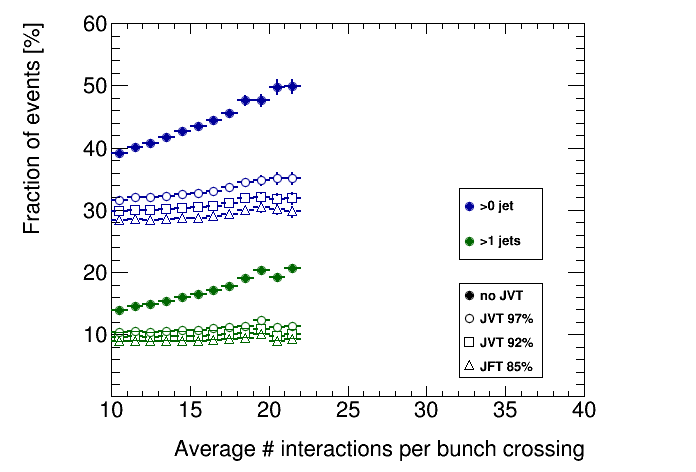
\includegraphics[trim=0.0cm 0cm 0cm 0cm,width=0.47\columnwidth]{FIGURES/Frac_njets_1and2}
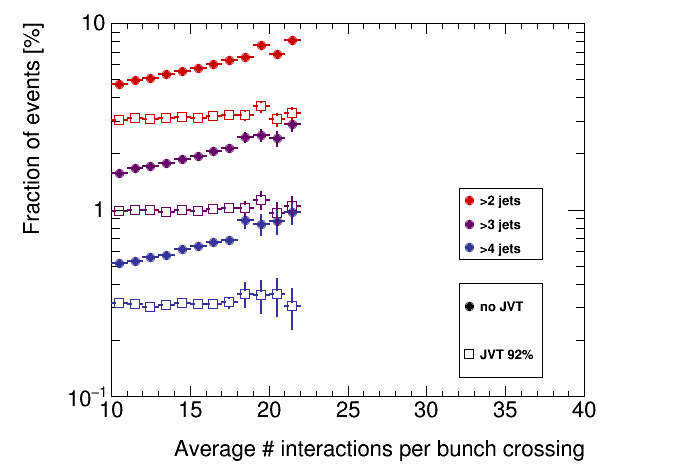
\includegraphics[trim=0.0cm 0cm 0cm 0cm,width=0.47\columnwidth]{FIGURES/Frac_njets_3to5}
\vspace{-0.2cm}
\end{center}
\caption{Fraction of events [\%] in data with at least 1 or 2 jets (left) and with at least 3, 4 or 5 jets (right) with respect to average number of interactions per bunch crossing with and without a cut on the JVT. Event selection requires a pair of leptons, and all jets have \pt~$>$~25\GeV. $L$~=~3.2~fb$^{-1}$ and $\sqrt s$~=~13\TeV.}
\label{Figure:JVF_Dependency_Run2} 
\end{figure}
%%%%%%%%%%%%%%%%%%%%%%%%%%%%%%%%%%%%%%%%%%%%%%%%%%%%%%%%%%%%

\subsubsection{$b$-tagging}

Tagging of $b$-jets is done using the MV2c20 algorithm with the 70\% efficiency 
operating point. This algorithm is based on a neural network using 
the output weights of the JetFitter+IP3D, IP3D and SV1 algorithms as input.
This efficiency working point was favored by optimisation studies performed with MC15 simulated signal and background samples as described below.
Figure~\ref{fig:btagging} shows the $b$-jet multiplicity for the three tagging efficiency working points. 
Monte Carlo background distributions are shown after same-sign lepton pair requirement.

\begin{figure}[htb!!]
\begin{center}
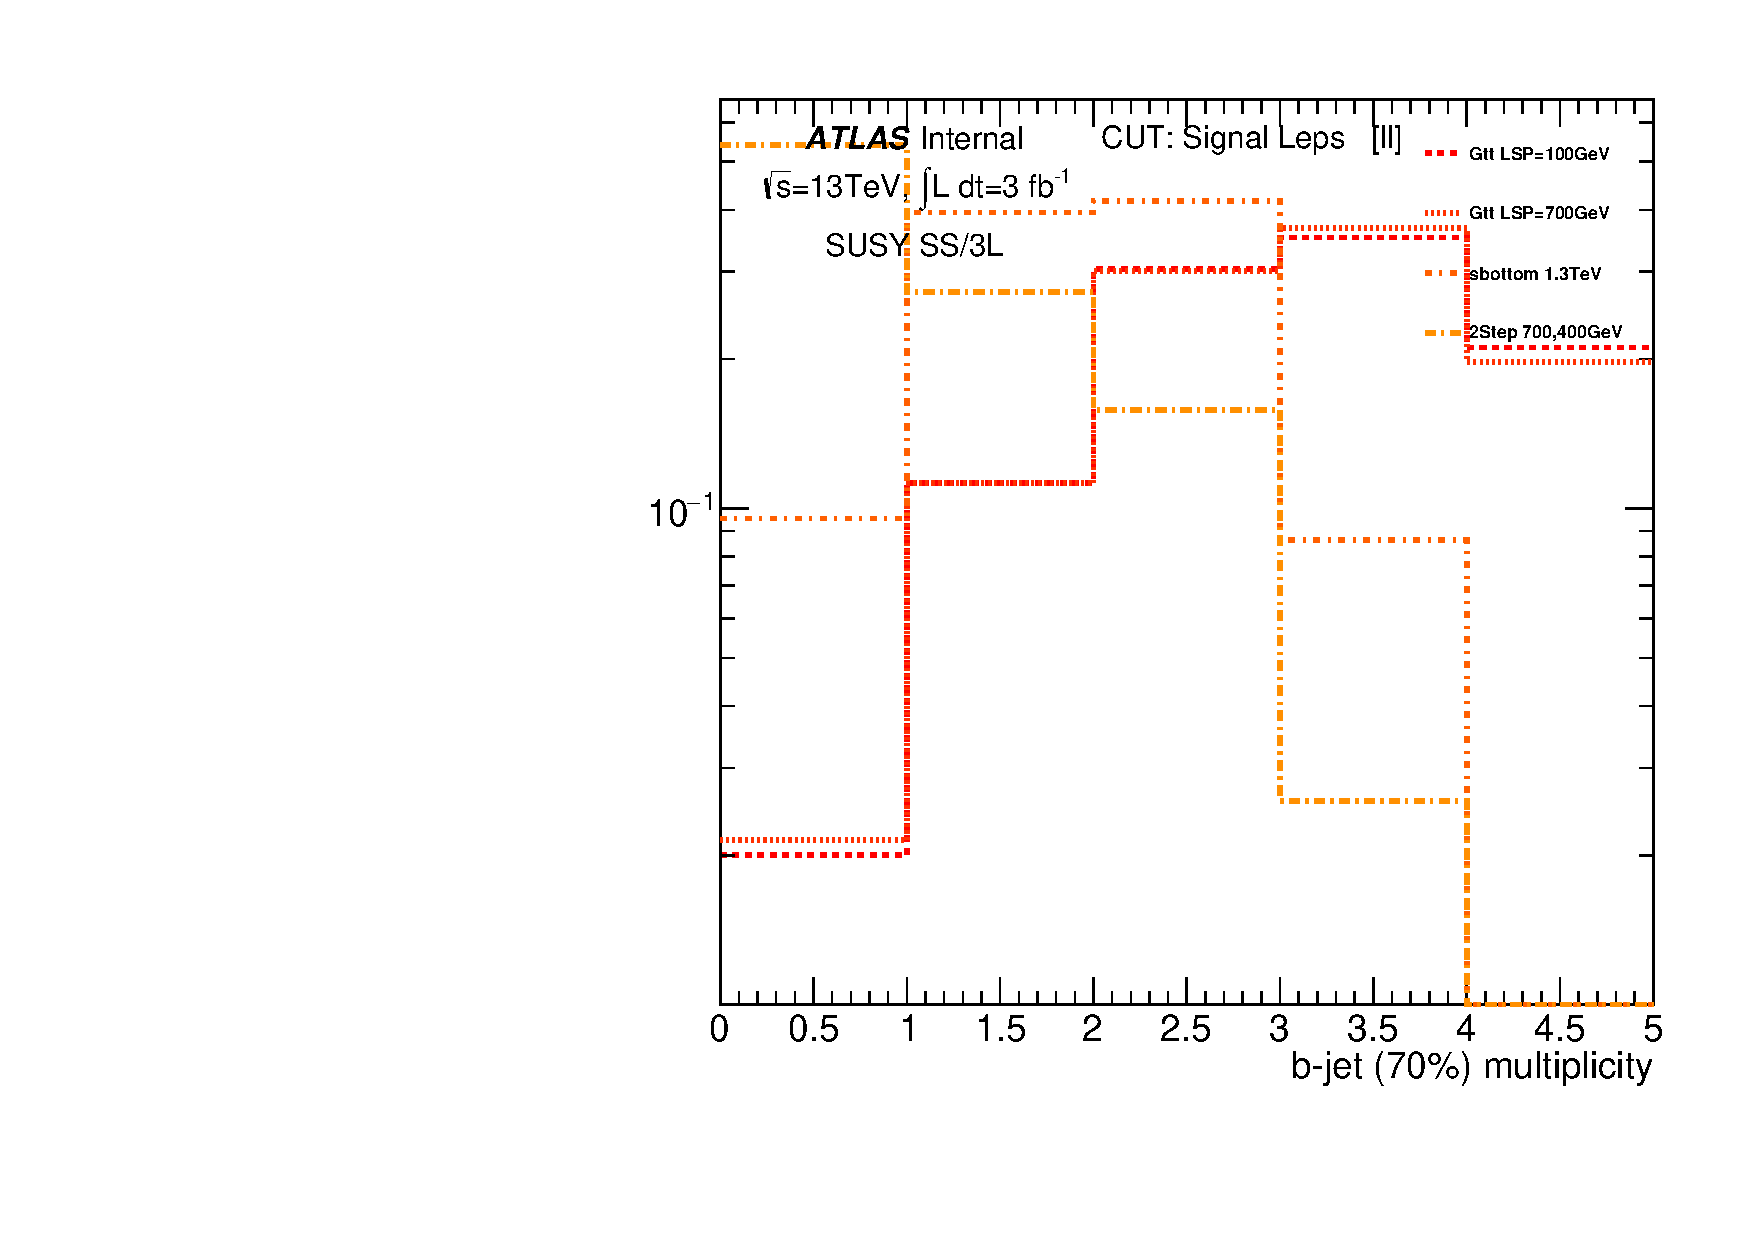
\includegraphics[width=0.3\textwidth]{FIGURES/BTAGGING/02_CutLEP_ll_NB1JET_signals.pdf} 
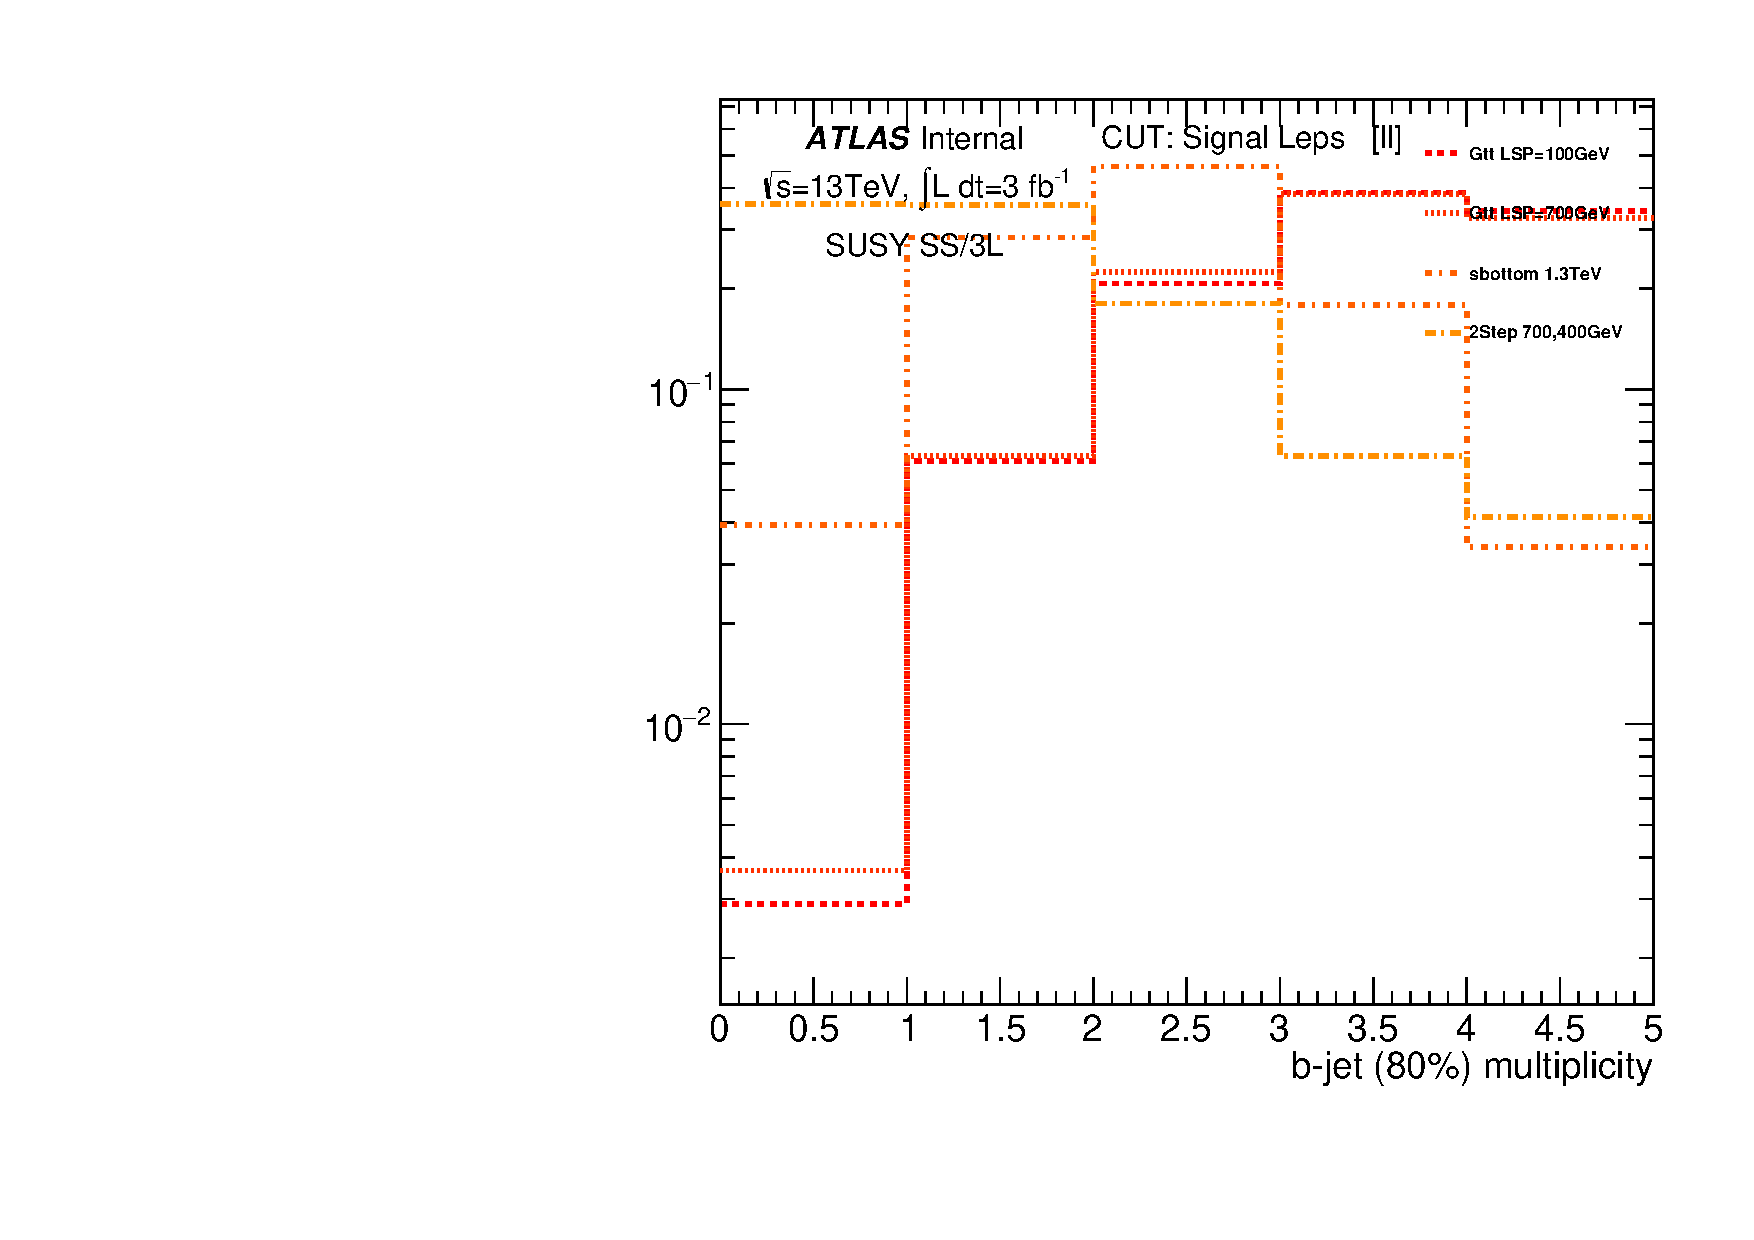
\includegraphics[width=0.3\textwidth]{FIGURES/BTAGGING/02_CutLEP_ll_NB2JET_signals.pdf}
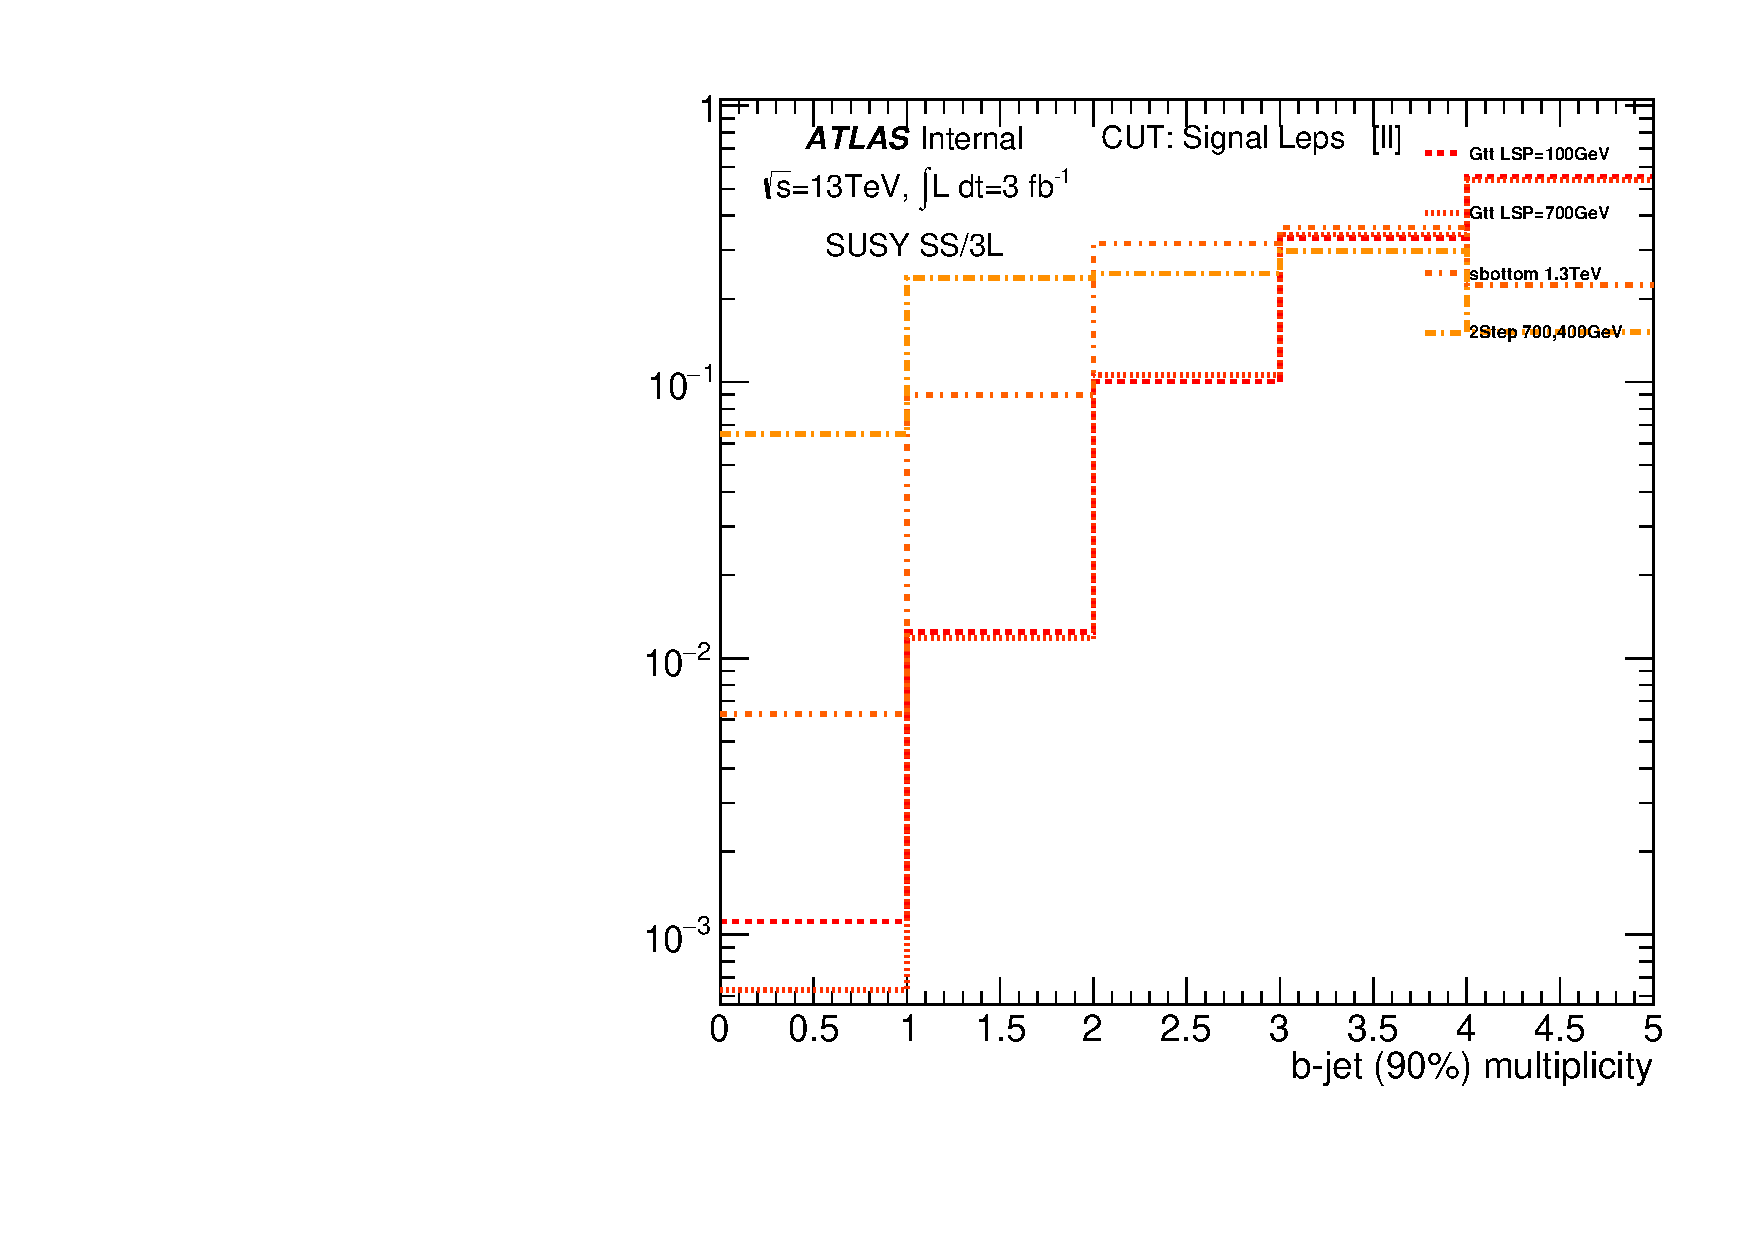
\includegraphics[width=0.3\textwidth]{FIGURES/BTAGGING/02_CutLEP_ll_NB3JET_signals.pdf}\\ 
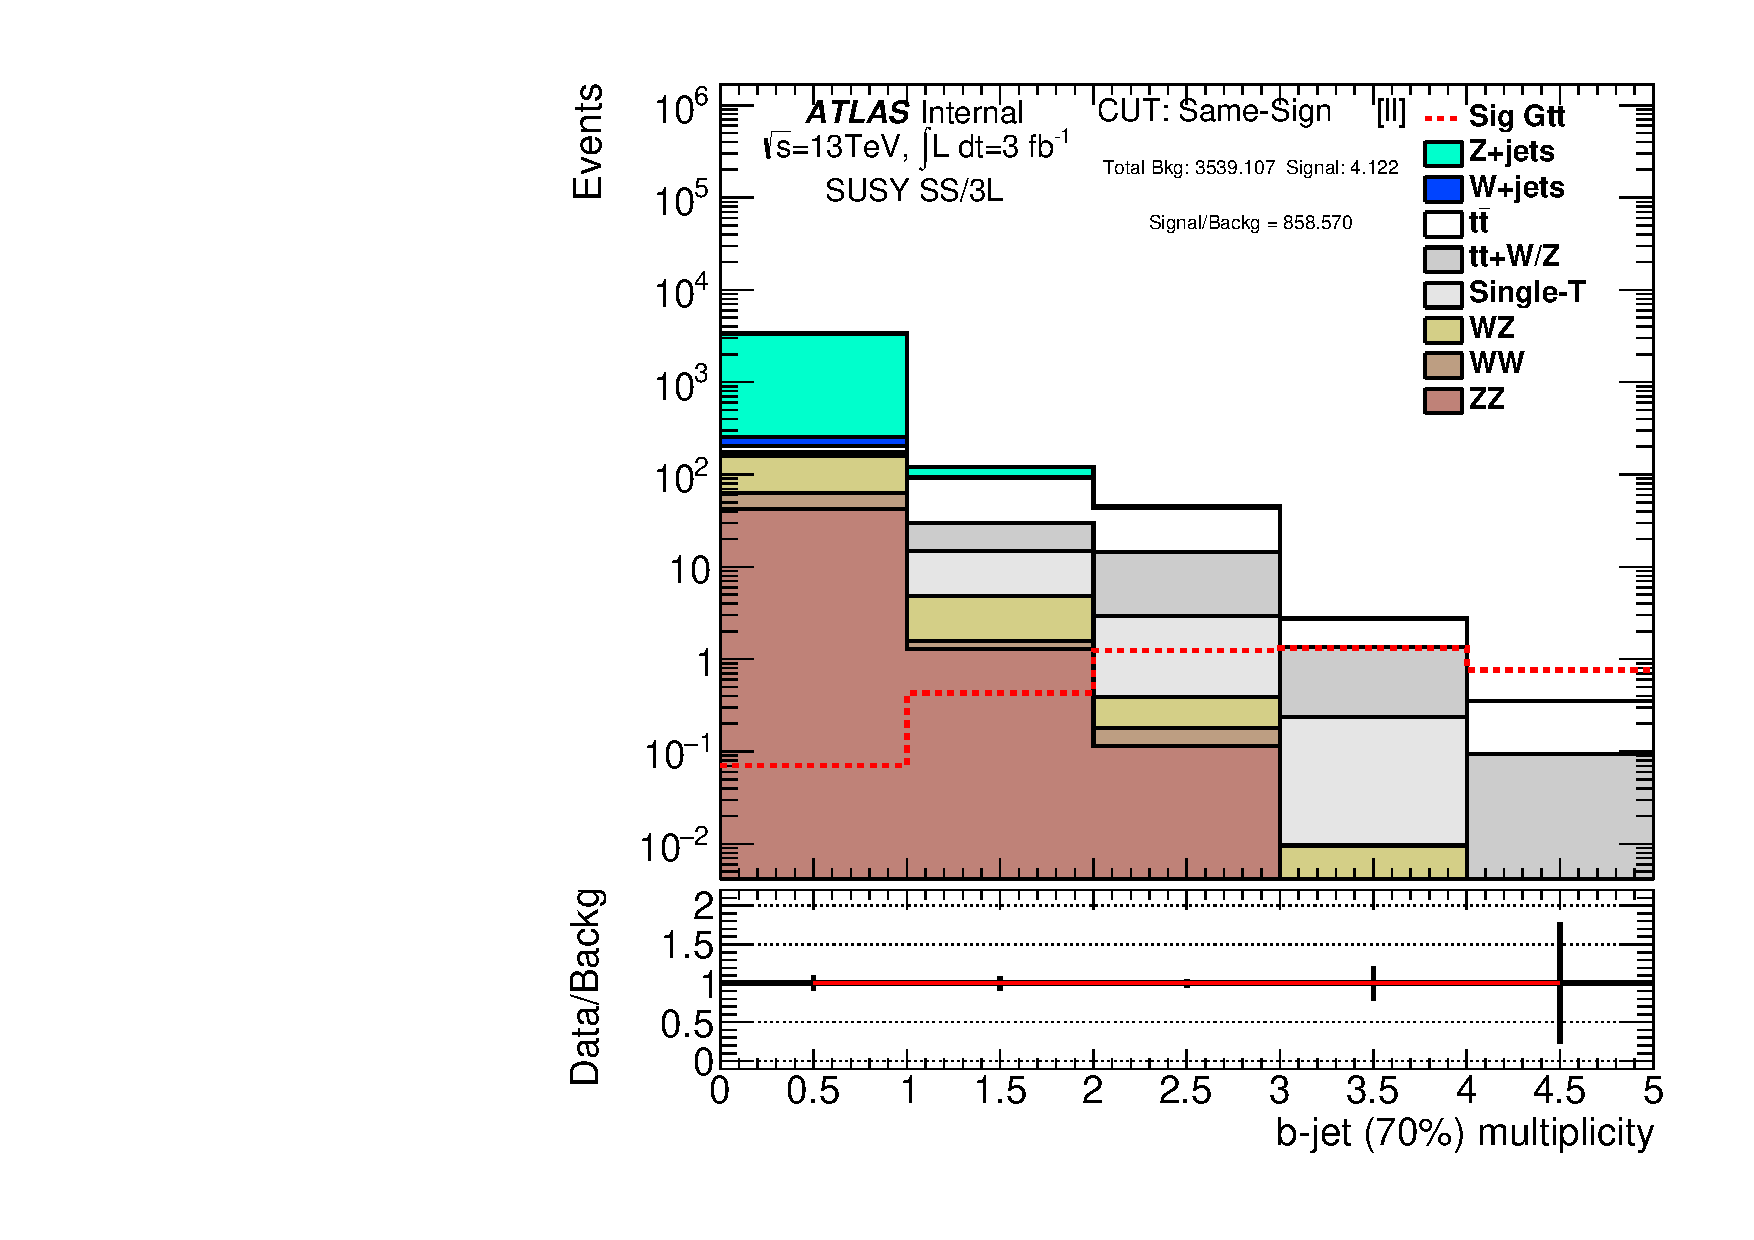
\includegraphics[width=0.3\textwidth]{FIGURES/BTAGGING/05_CutSS_ll_NB1JET.pdf}
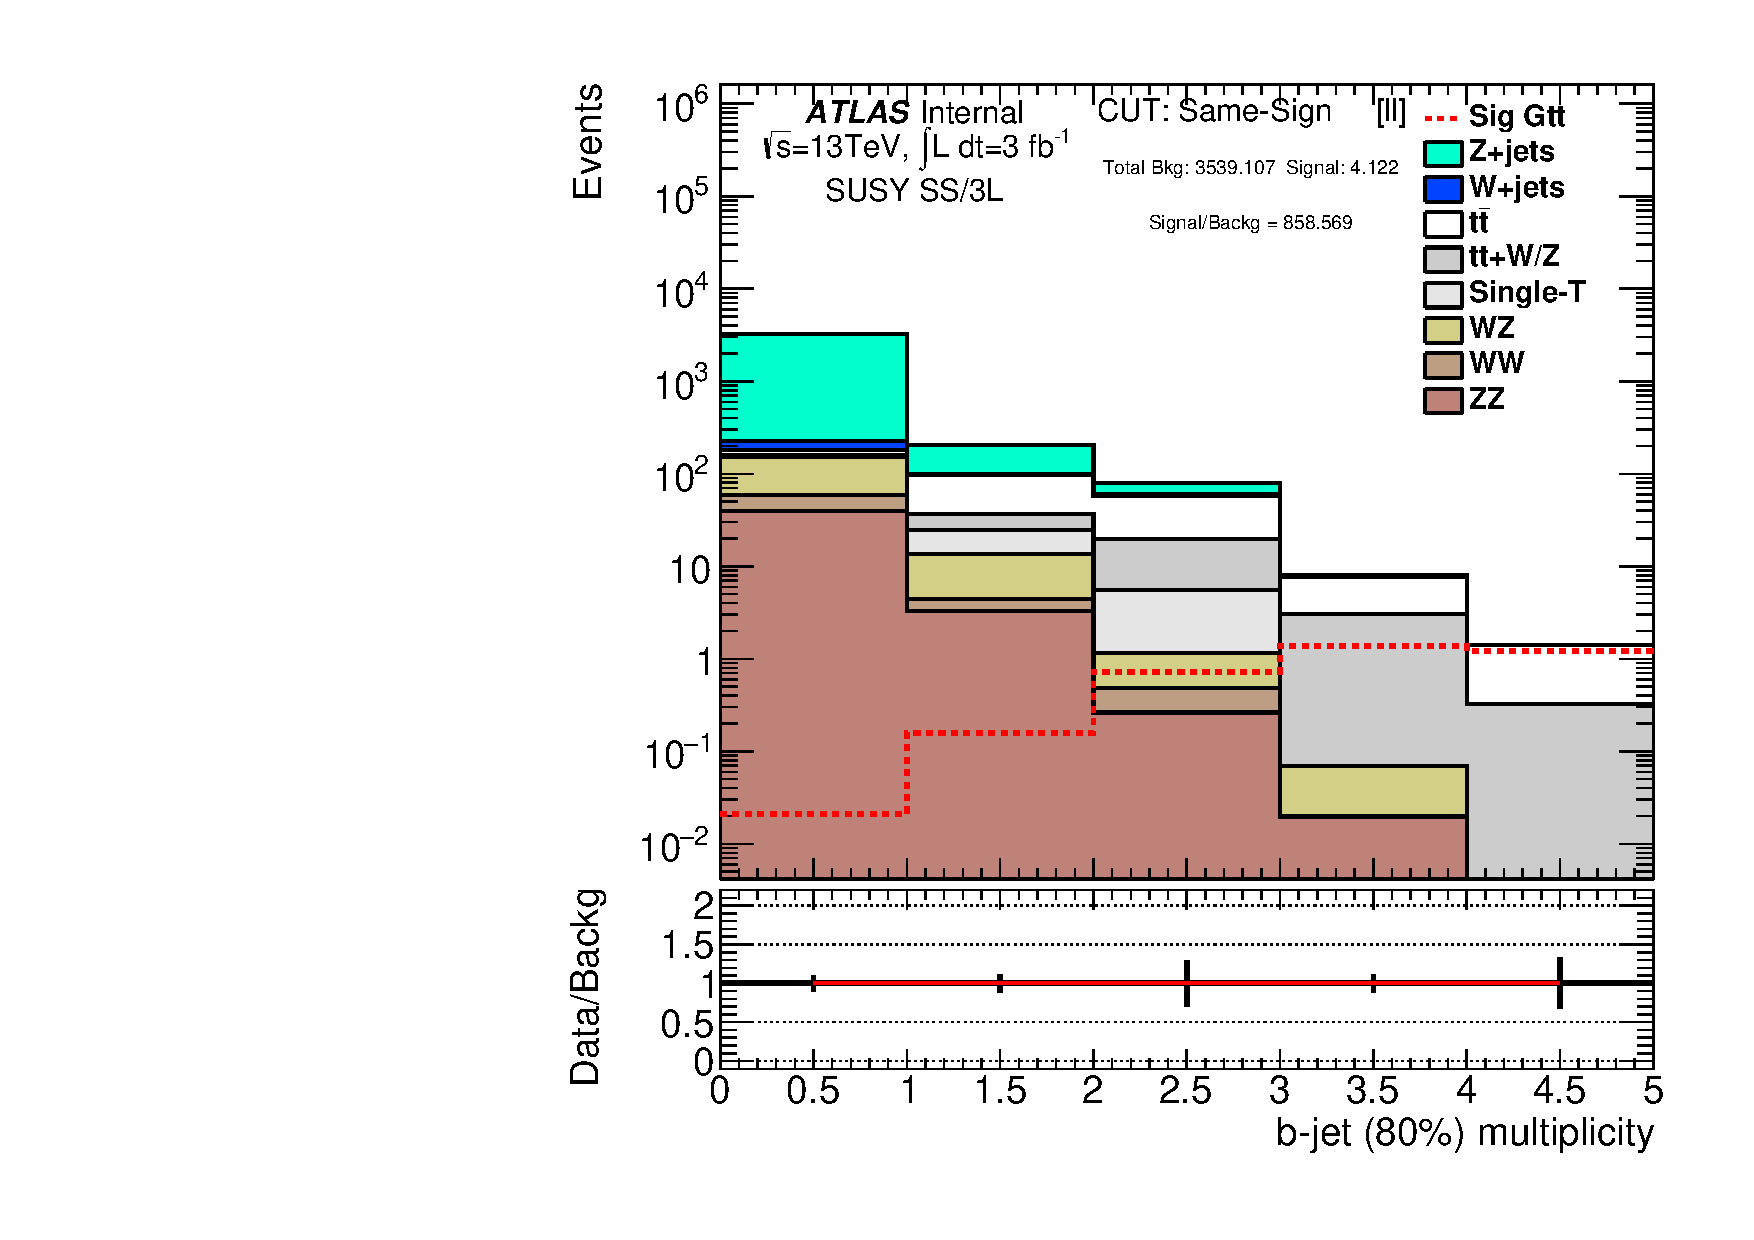
\includegraphics[width=0.3\textwidth]{FIGURES/BTAGGING/05_CutSS_ll_NB2JET.pdf}
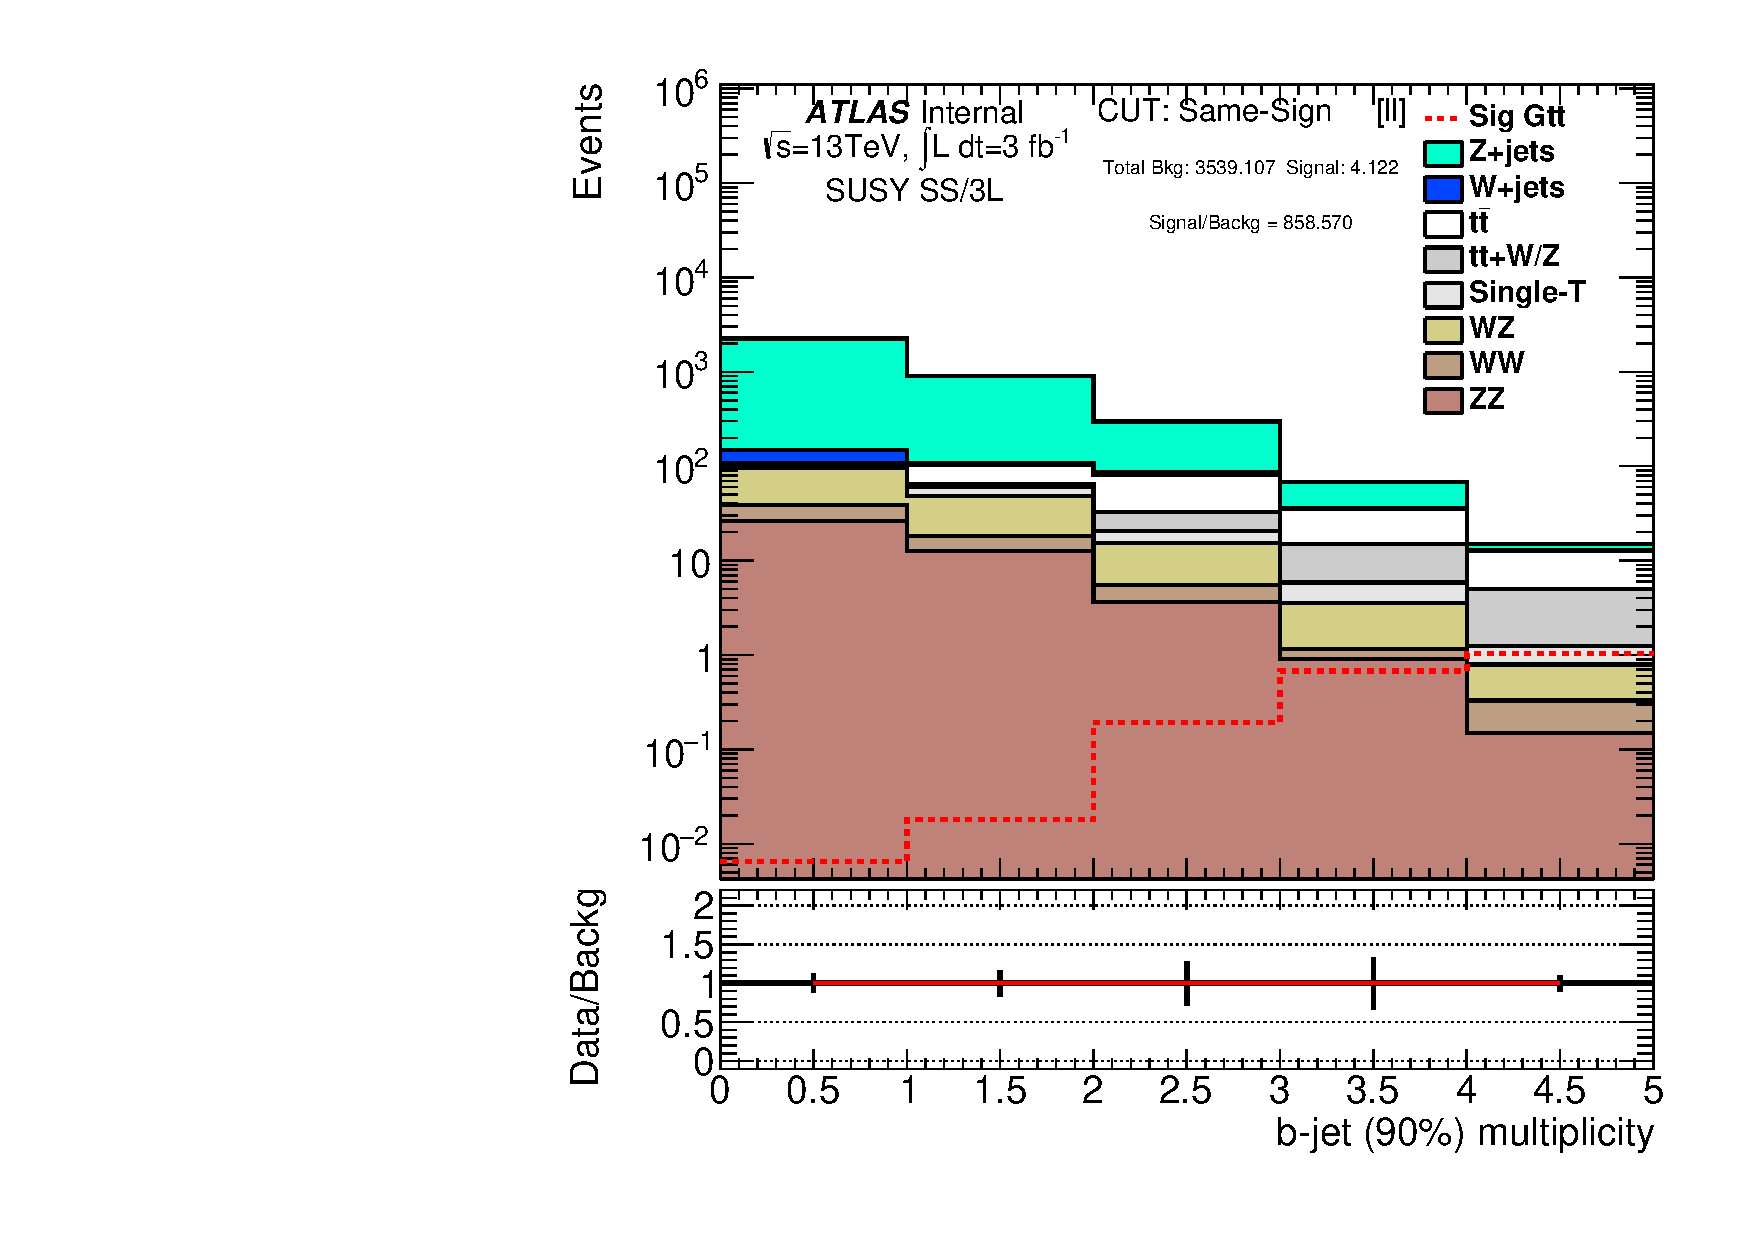
\includegraphics[width=0.3\textwidth]{FIGURES/BTAGGING/05_CutSS_ll_NB3JET.pdf} 
\end{center}
\vspace{-0.2cm}
\caption{$b$-jet multiplicity for three different tagging efficiency working points, left 70\%, center 80\%, right 90\%.
Signals shapes are shown on the top figures, and stacked background expectations for an integrated luminosity of 3~fb$^{-1}$ are shown on the bottom plots.}
\label{fig:btagging}
\end{figure}

Different signal models described earlier on this document are expected to contain different heavy flavour jet multiplicities.
Therefore the choice of the most performant $b$-jet tagging efficiency working point was made by looking into regions that emulate the signal regions that would eventually be used in the analysis.
Table~\ref{tab:btaggingSR} describes the six different signal-like regions used on this optimisation. 

%%%%%%%%%%%%%%%%%%%%%%%%%%%%%%%%%%%%%%%%%%%%%%%%%%%%%%%%%%%%%
\begin{table}[htb!]
\caption{Signal-like region selections used for the $b$-jet efficiency working point optimisation.}
\label{tab:btaggingSR}
\begin{center}
\begin{tabular}{l|c|c|l}
                & \#$\ell$ & \#$b$-jets & Other cuts                          \\ \hline \hline
  SR-3$b$       & $\geq 2$ & $\geq 3$   & $N^{40}_j \geq 6$                    \\
  SR-3$b$ Soft  & $\geq 2$ & $\geq 3$   & $N^{20}_j \geq 7$ \&\& MET$>$150~GeV \\\hline
  SR-1$b$       & $\geq 2$ & $\geq 1$   & $N^{50}_j \geq 4$ \&\& MET$>$150~GeV (!SR3b)\\
  SR-1$b$ Incl  & $\geq 2$ & $\geq 1$   & $N^{40}_j \geq 4$ \&\& MET$>$150~GeV \\\hline
  SR-0$b$- 5j   & $\geq 2$ & $== 0$     & $N^{50}_j \geq 5$ \&\& MET$>$100~GeV \\
  SR-0$b$- 3j   & $\geq 2$ & $== 0$     & $N^{40}_j \geq 3$ \&\& MET$>$200~GeV \\ \hline
\end{tabular}
\end{center}
\end{table}
%%%%%%%%%%%%%%%%%%%%%%%%%%%%%%%%%%%%%%%%%%%%%%%%%%%%%%%%%%%%
         
\begin{figure}[htb!!]
\begin{center}
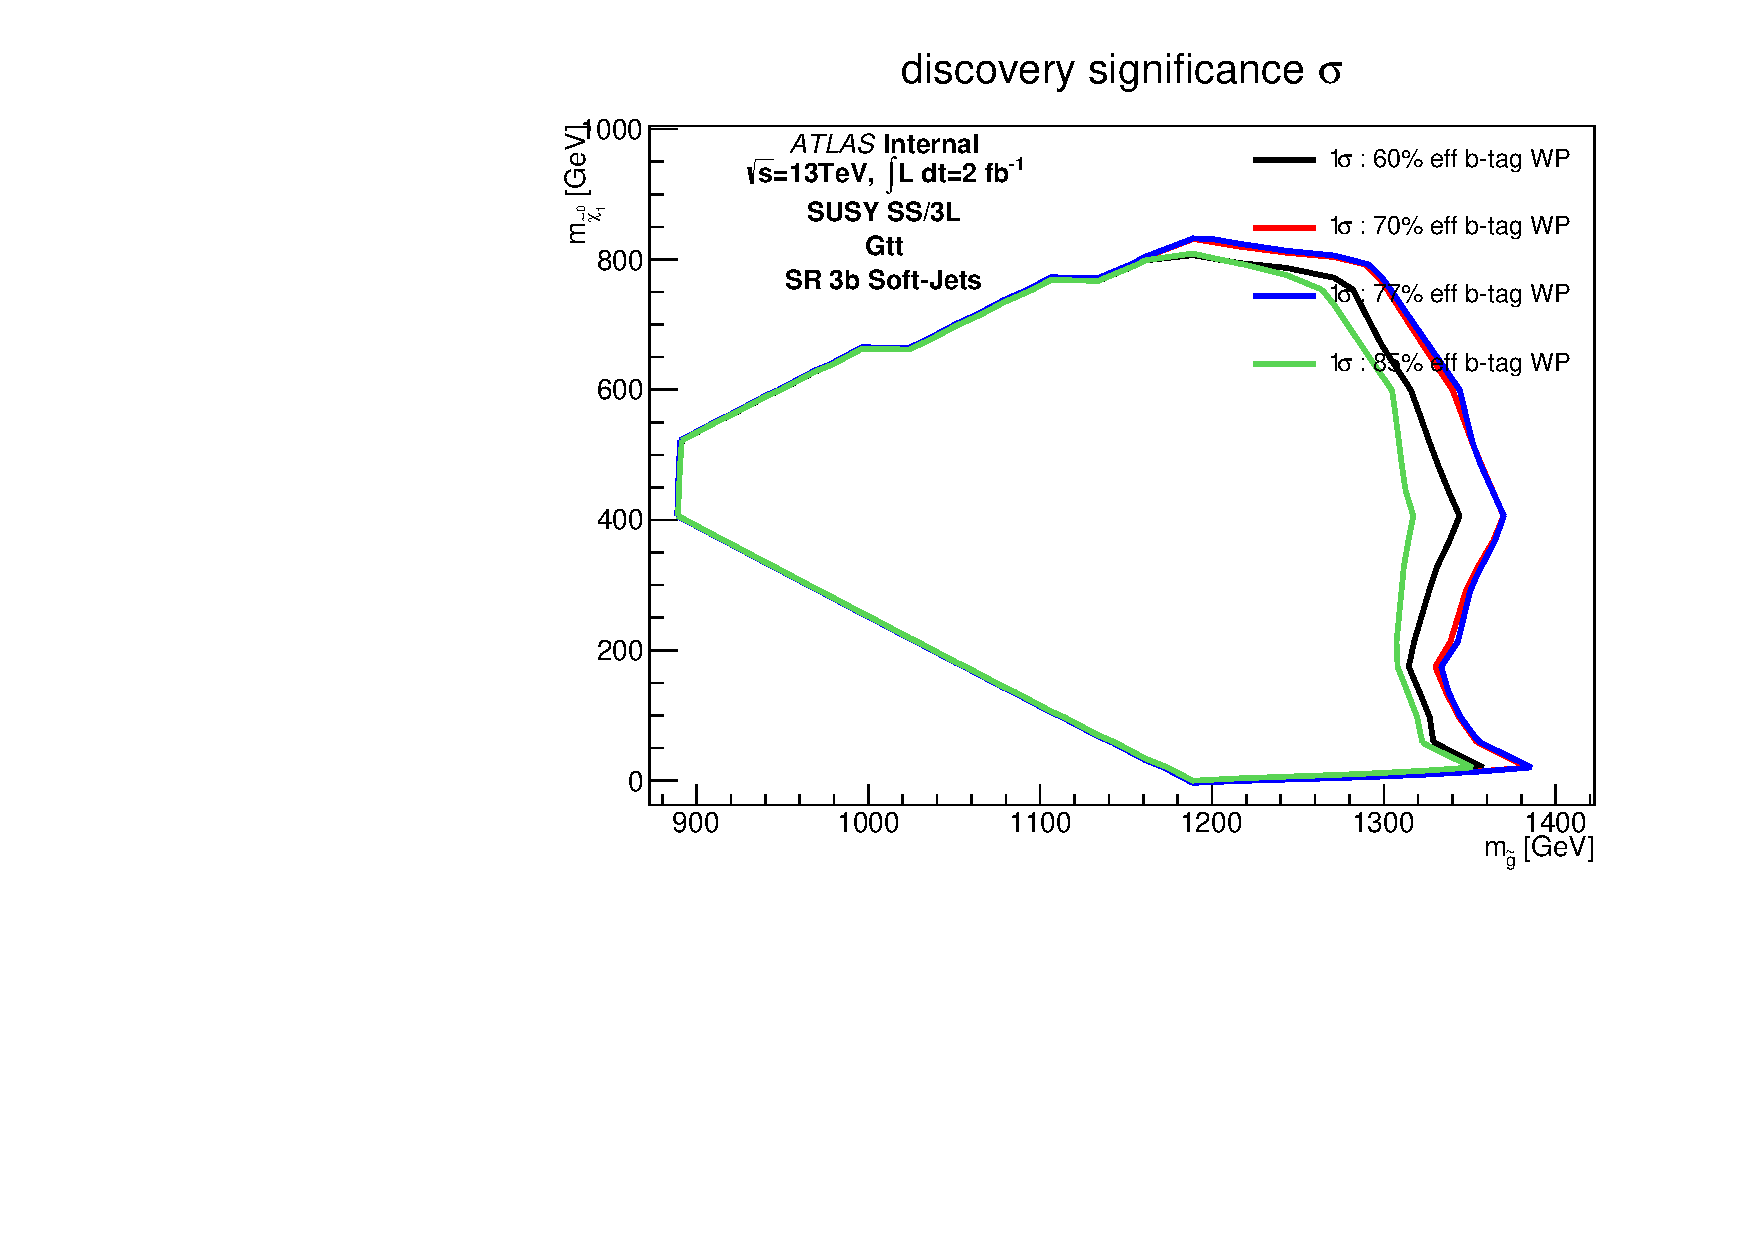
\includegraphics[width=0.45\textwidth]{FIGURES/BTAGGINGMC15/L2fb/plot_significance_gtt_CutSR3BS60_all.pdf}\\
%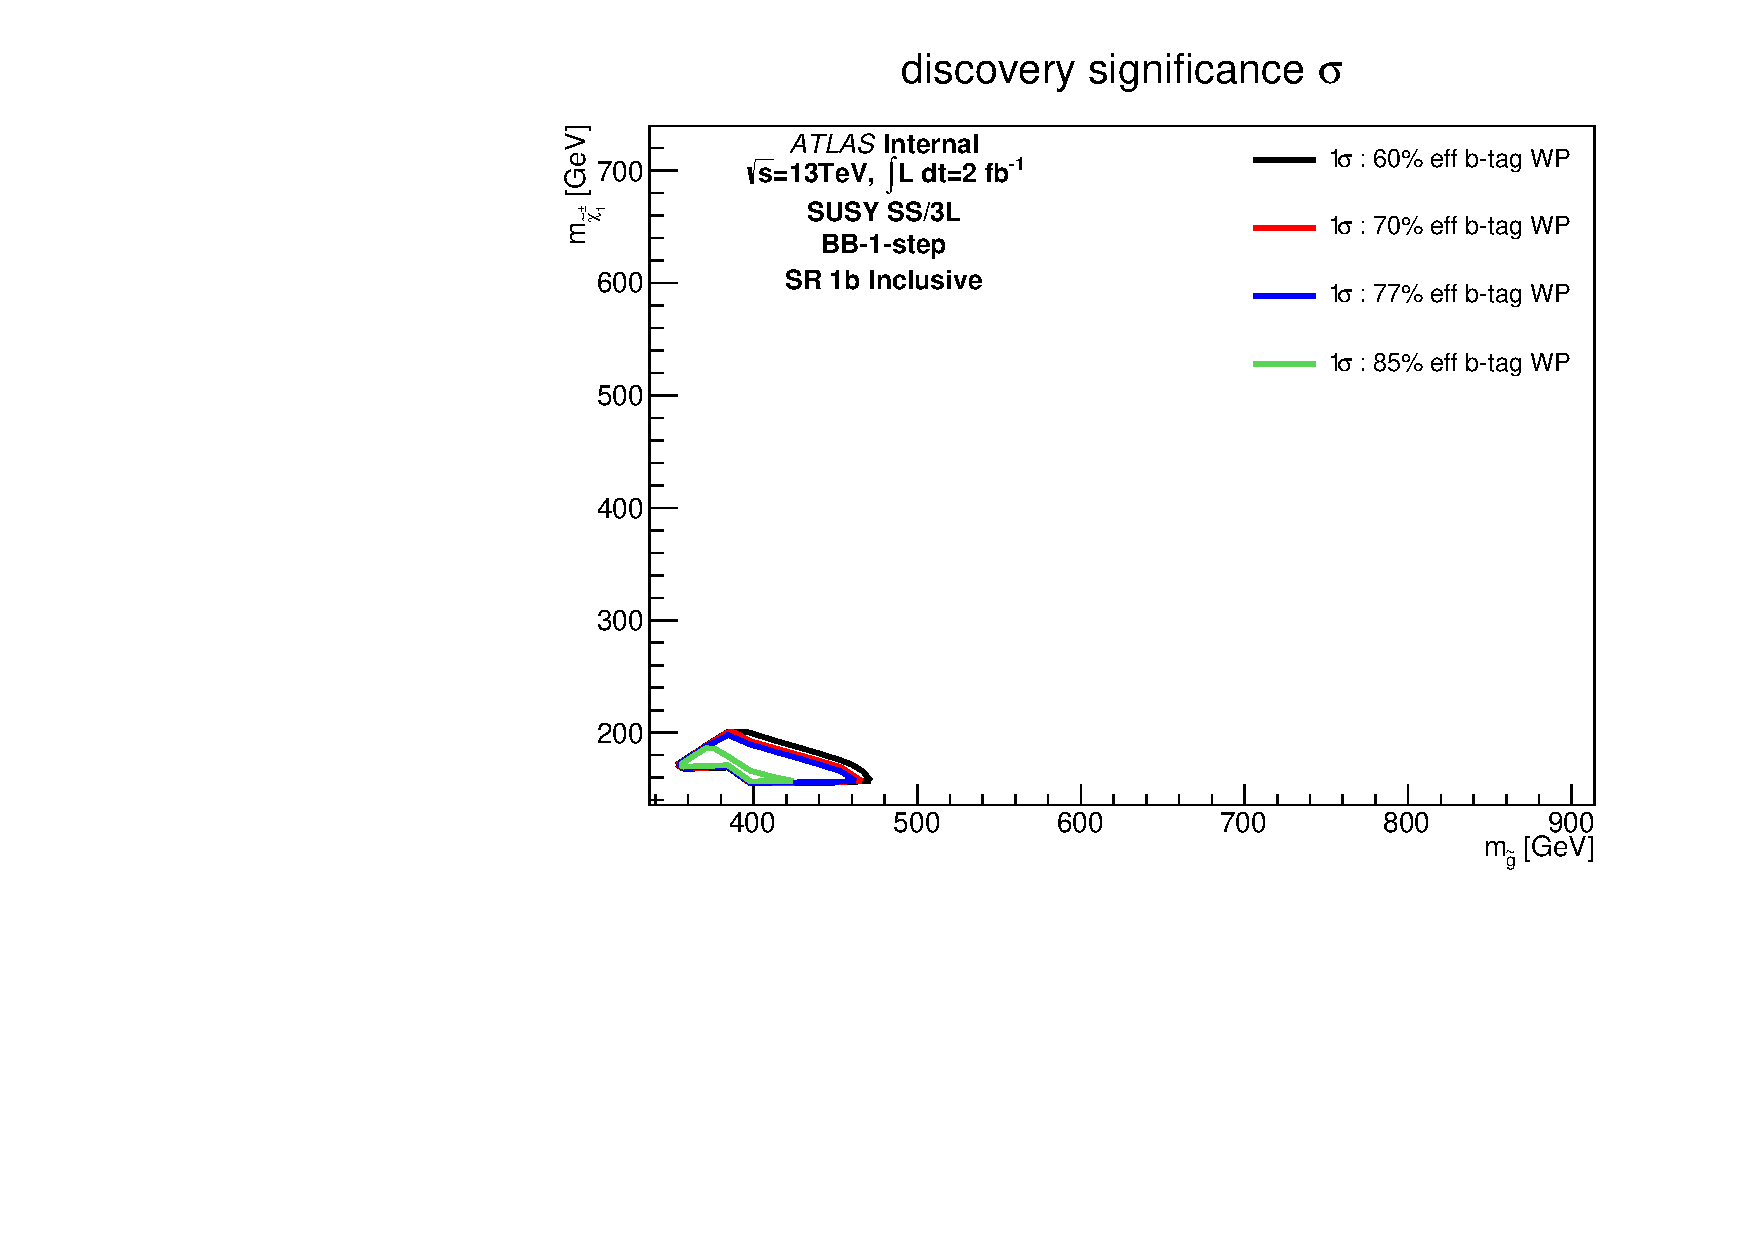
\includegraphics[width=0.3\textwidth]{FIGURES/BTAGGINGMC15/L2fb/plot_significance_bb1step_CutSR1BI60_all.pdf}\\
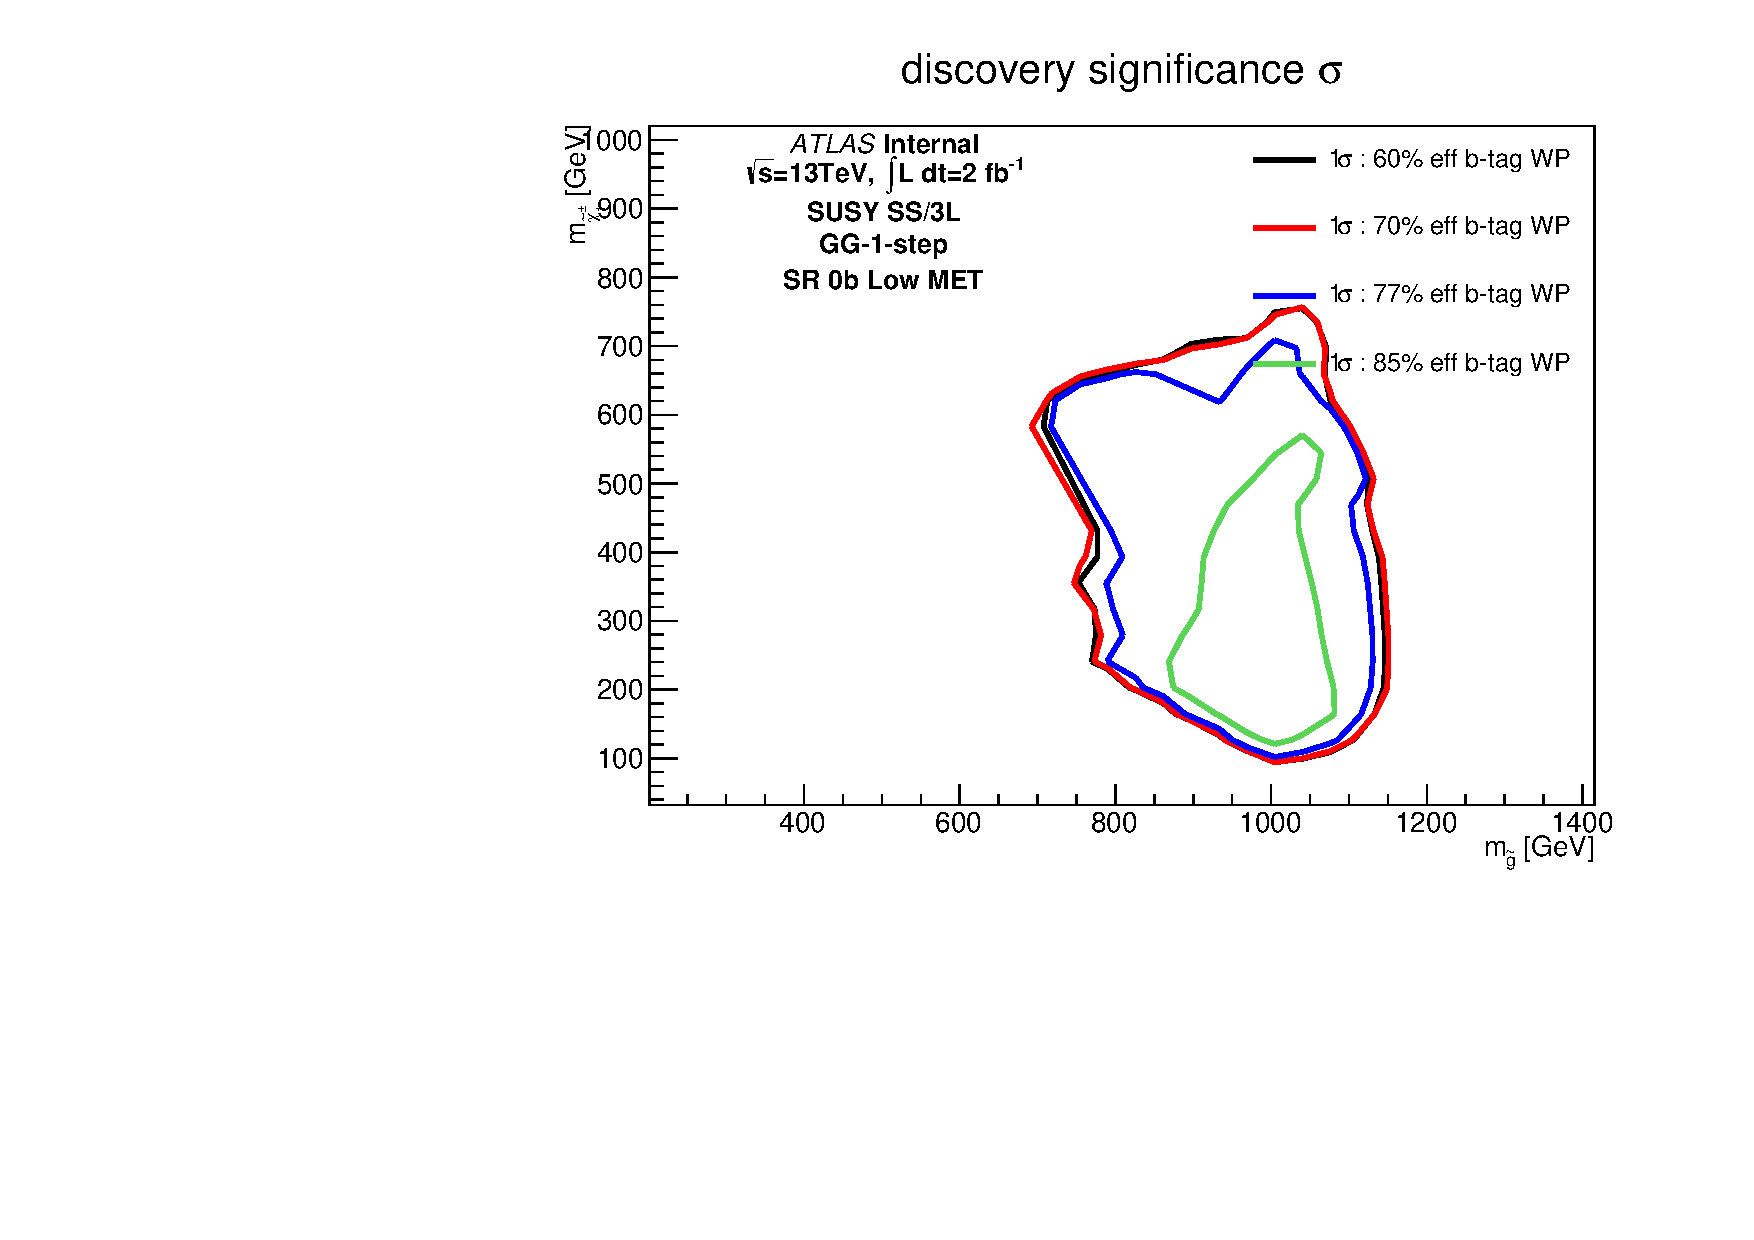
\includegraphics[width=0.45\textwidth]{FIGURES/BTAGGINGMC15/L2fb/plot_significance_gg1step_CutSR0BL60_all.pdf}        
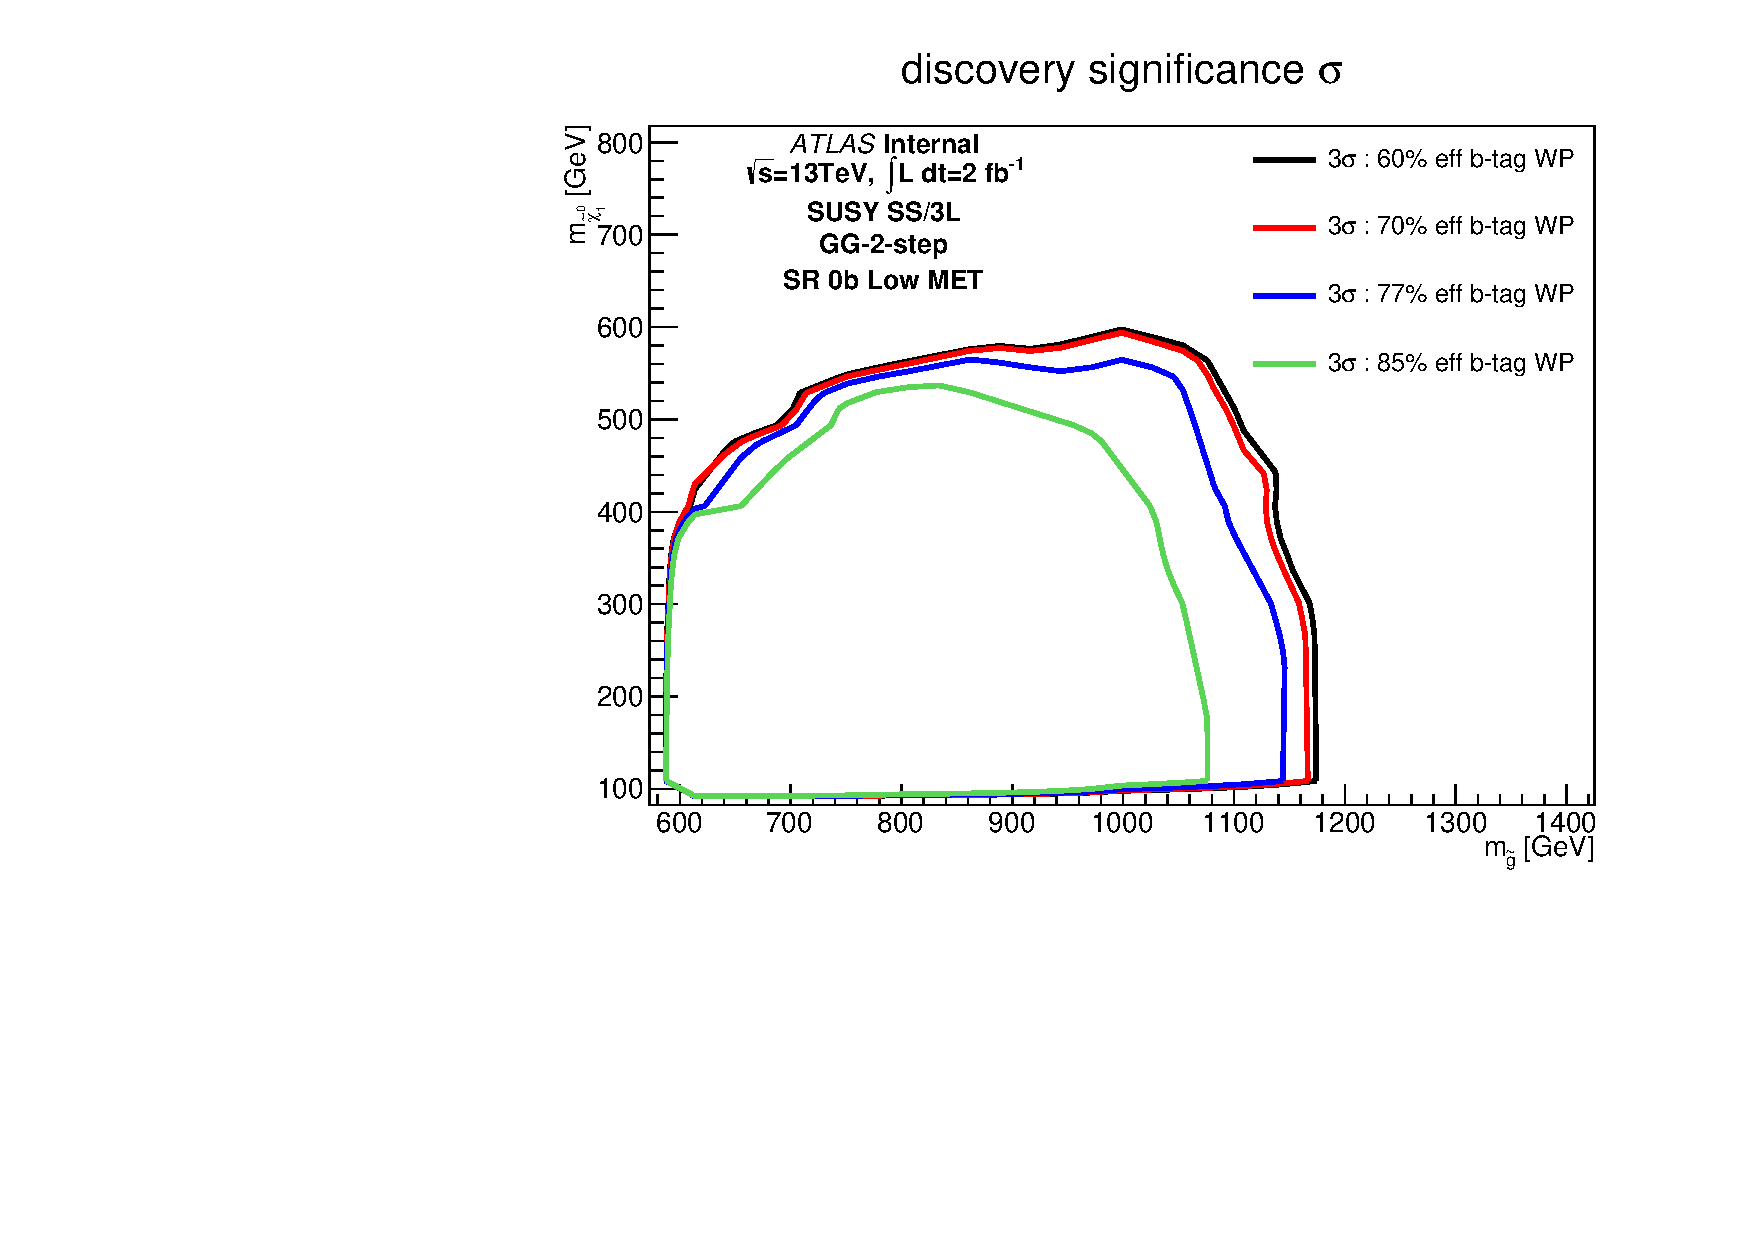
\includegraphics[width=0.45\textwidth]{FIGURES/BTAGGINGMC15/L2fb/plot_significance_gg2step_CutSR0BL60_all.pdf}          
\end{center}
\vspace{-0.2cm}
\caption{Gaussian discovery signal significance for the various signal-like regions where the different models are sensitive.
Three signal models are tested: the gluino-stop off-shell (top), the gluino production mediated by charginos (bottom left) and the 2-step gluinos via charginos (bottom right).
$b$-jet tagging efficiency working points supported by the heavy flavour working group are 60\%(black), 70\%(red), 77\%(blue) and 85\%(green).
Expectations are estimated assuming an integrated luminosity of 2~fb$^{-1}$ of 13~TeV.}
\label{fig:btaggingGrid}
\end{figure}

Figure~\ref{fig:btaggingGrid} shows the discovery signal significance using a simple Gaussian approximation ($S/\sqrt{S+(\Delta B)^2}$) for different choices of the $b$-tagging working point (60\%, 70\%, 77\% and 85\%) with a flat assumption on the background uncertainty of 40\%. The signal region for each of the models was chosen based on the highest sensitivity.
The 3$b$ Soft signal-like region was found to be the most performant for the gluino-stop off-shell production, 
and the 0$b$-5j signal-like region for the gluino production mediated by charginos as well as the 2-step 
gluino production mediated by gauginos. 
%As more signal simulations become available similar studies would be performed for sbottom direct production and gluinos (and squarks) 2-step models mediated via sleptons.
The 70\% $b$-tagging efficiency working point is chosen since it is the best compromise allowing to reach good sensitivity in the different tested signal models.

%Similar studies with detailed information comparing the performance of previous MV1 (rel-19) tagger and MV2c20 (rel-20) are shown in Appendix~\ref{app_btagging}.

\subsection{Leptons}
\label{sec:objects_leptons}

This section summarizes the electron and muon object selection, as well as developments done in the optimization of the
lepton isolation and electron acceptance cuts.

\subsubsection{Electrons}
\label{sec:objects_electrons}

The electron selection is summarized in Table~\ref{tab:lepdef}. The Egamma CP group recommends the likelihood-based electron identification~\cite{ATLAS-CONF-2014-032} for Run-2, since it provides a factor of two better background rejection than the cut-based identification.
Four working points ({\tt VeryLooseLH}, {\tt LooseLH}, {\tt MediumLH}, {\tt TightLH}) are available for LH electrons.

Pre-selected electrons must satisfy the {\tt LooseLH} requirements and have $E_\mathrm{T}>10$~GeV and $|\eta|<2.47$. 
Electrons in the LAr crack region ($1.37<|\eta|<1.52$) are rejected to reduce the contribution from non-prompt electrons. 
A requirement on the transverse impact parameter of $|d_0/\sigma(d_0)|<5$ (as recommended by TrackingCP) is also applied to pre-selected electrons and helps reducing the contribution from charge mis-identification. 
Signal electrons are additionally required to pass the isolation cuts defined in~\ref{sec:isolation} 
as well as the {\tt TightLH} identification criteria and standard requirements of the longitudinal impact parameter ($|z_0 \cdot sin(\theta)|<$ 0.5 mm, as recommended by TrackingCP).

A multiplicative event weight is applied for each signal electron in MC to the overall event weight 
in order to correct for differences in efficiency between data and MC as recommended by the Egamma group.

\subsubsection{Muons}
\label{sec:objects_muons}

The muon selection is summarized in Table~\ref{tab:lepdef}. The Run-2 muon reconstruction is performed by the so-called \textit{third chain}: 
it has been designed to combine the best features of the Run-1 STACO and MUID chains to provide the best performance. 
The following muon selection working points are supported:
{\tt Tight}, {\tt Medium}, {\tt Loose} and {\tt VeryLoose}. 

Pre-selected muon candidates must pass the {\tt Medium} muon quality cuts and have  $p_\mathrm{T} > 10\GeV$ and $|\eta| < 2.4$.
A smearing procedure is applied to the muon $p_\mathrm{T}$.  
A multiplicative event weight is applied for each selected muon in MC to the overall event weight in order to correct for differences in efficiency between data and MC as recommended by the Muon CP group. 

Finally, signal muon candidates are required to pass the isolation cuts defined in~\ref{sec:isolation} as well as the requirements on the impact parameter of $|d_0/\sigma(d_0)|<3$ and $|z_0 \cdot sin(\theta)|<$ 0.5 mm, as recommended by TrackingCP.


Note that events with ``cosmic'' muons, or ``Bad'' muon are vetoed as described in Section~\ref{sec:presel}.


%%%%%%%%%%%%%%%%%%%%%%%%%%%%%%%%%%%%%%%%%%%%%%%%%%%%%%%%%%%%%
\begin{table}[htb!]
\caption{Summary of the electron and muon selection criteria. The signal
  selection requirements are applied on top of the preselection. The
  lepton-jet isolation requirement is applied after electron-jet overlap
  removal.}
\label{tab:lepdef}
\begin{center}
    \begin{tabular}{|l|c|c|}
      \hline
      \hline
       & \textbf{Pre-selected Electron} & \textbf{Pre-selected Muon} \\
      \hline
      \hline
      Acceptance     & $\pt > 10\,\GeV, |\eta^\mathrm{clust}| < 2.47$  & $\pt > 10\,\GeV, |\eta| < 2.5$ \\
                     &  except $1.37<|\eta^\mathrm{clust}|<1.52$       & \\
      \hline
      Quality & {\tt LooseLLH} & {\tt{xAOD::Muon::Medium}} \\
%      \hline
%      Impact parameter &  $|d_0/\sigma(d_0)|<$ 5.0 & - \\
      \hline
      $\ell$-jet Isolation      & $\Delta{}R(e,jet)$~$>$~0.4 & $\Delta{}R(\mu,jet)$~$>$~0.4 \\
      \hline
      Impact parameter & $|d_0/\sigma(d_0)|<5.0$  & \\
      \hline\hline
       & \textbf{Signal Electron} & \textbf{Signal Muon} \\
      \hline
      \hline
      Quality & {\tt TightLLH} & -\\
       & $|\eta|<2.0$  & -\\
            \hline
      Isolation                & ``FixedCutTight '' & ``FixedCutTightTrackOnly'' \\
      \hline
      Impact parameter & $|z_0 \cdot sin(\theta)|<$ 0.5 mm   & $|z_0 \cdot sin(\theta)|<$ 0.5 mm \\ 
                       &                                     & $|d_0/\sigma(d_0)| < 3.0$\\
     \hline
\end{tabular}
\end{center}
\end{table}
%%%%%%%%%%%%%%%%%%%%%%%%%%%%%%%%%%%%%%%%%%%%%%%%%%%%%%%%%%%%


\subsubsection{Lepton isolation}
\label{sec:isolation}

The isolation working points proposed from this analysis were accepted by the ATLAS Isolation forum and implemented as officially supported working points in the {\tt IsolationSelectionTool}. Unless otherwise stated, the following isolation working points are used in the analysis:
\begin{itemize}
\item Electrons: {\tt TightLLH}, ptvarcone20/\pt$<$0.06 and topoetcone20/\pt$<$0.06 (``FixedCutTight'')
\item Muons: ptvarcone30/\pt\ $<0.06$ (``FixedCutTightTrackOnly'')
\end{itemize}
%Note that no isolation scale factors are used so far in the analysis, but will be released by the EGamma and Muon combined performance groups with the whole 2015 dataset.
Isolation scale factors determined by the CP groups for these working points are applied. 

More details on the isolation studies performed in the context of this analysis can be found in Appendix~\ref{app:iso}.



\subsubsection{Electron acceptance}
\label{sec:eleAcceptance}

Dedicated studies have been conducted to evaluate the impact of a reduction of the $|\eta|$ coverage for electrons. 
This is motivated by the fact that the largest contributions from charge-flip and fake lepton backgrounds 
are observed at $|\eta|>2$ and in the LAr crack region ($1.37<|\eta|<1.52$), 
due to poorer detector resolution or increased amount of material in these regions. 

Table~\ref{tab:eleEta} shows the impact on the expected event yields when reducing the electron $|\eta|$ acceptance 
for the two leading electrons (taking a reference the case of $|\eta|<2.3$). The event selection applied to compute those numbers 
requires SS/3L, at least 3 jets with $\pt > 30$~GeV and $m_{ee}$ outside the 84-98~GeV range to reduce the contribution 
from charge flips. 

%%%%%%%%%%%%%%%%%%%%%%%%%%%%%%%%%%%%%%%%%%%%%%%%%%%%%%%%%%%%%
\begin{table}[htb]
\caption{Relative decrease in the event yield when reducing the $|\eta|$ acceptance for the two leading electrons with respect to $|\eta|<2.3$. The reference is considered to be $|\eta|$~$<$~2.47, and the crack region is excluded in all the cases. Numbers are shown for the event selection described in the text and separately for events with 1 or more $b$-jets.}
\label{tab:eleEta}
\begin{center}
    \begin{tabular}{|l|c|c|c|c|c|} \hline
                   & Prompt SS & $\ttbar +W$ & Gtt (G900\_L100) & Non-prompt leptons & Charge flip \\ \hline\hline
==1$b$, $|\eta|<1.37$ & 14\% & 16\% & 12\%  & 28\% & 69\% \\
==1$b$, $|\eta|<2.0$  & 5.4\%  & 6\%  & 7\%&  11\% & 37\% \\ 
==1$b$, $|\eta|<2.3$  & 0.4\%  & 1.5\%  & 4.7\%&  3.6\% &  11\% \\ \hline
$>$1$b$, $|\eta|<1.37$ & 13\% & 18\% & 10\%  & 44\% & 66\% \\
$>$1$b$, $|\eta|<2.0$  & 4.3\%  & 6.5\%  & 2.9\%&  21\% &  30\% \\ 
$>$1$b$, $|\eta|<2.3$  & 1.3\%  & 1.5\%  & 0.3\%&  8\% &  5.8\% \\  \hline
\end{tabular}
\end{center}
\end{table}
%%%%%%%%%%%%%%%%%%%%%%%%%%%%%%%%%%%%%%%%%%%%%%%%%%%%%%%%%%%%

As shown, reducing the acceptance to $|\eta|<2.0$ would reduce the contribution from processes with prompt 
SS/3L by 6.5\% or less, but the reduction in non-prompt leptons (11-21\%) and charge flip (30-37\%) is quite larger. 
Reducing the acceptance more severely for the two leading electrons to $|\eta|<1.37$ would reduce the non-prompt and 
charge flip components by 28-44\% and $\sim$69\%, respectively, with a reduction of only 13-18\% for prompt SS/3L processes. 

Therefore, this study proves that additional rejection against some of the main backgrounds affecting the analysis can be achieved 
by reducing the $|\eta|$ acceptance of the electrons. 
As illustrated in Table~\ref{tab:lepdef} we chose in conclusion to reject electrons with $|\eta|>2.0$ or in the EM calorimeter cracks ($1.37<|\eta_\text{cluster}|<1.52$). 
Note that these requirements are applied to electrons regardless of the lepton multiplicity of the event.

\subsection{Overlap removal}
\label{sec:objects_overlap_removal}

According to the above definitions, one single final state object may fall in more than one category, being therefore effectively double-counted. 
For example, one isolated electron is typically reconstructed both as an electron and as a jet. A procedure to remove overlaps between final state objects was therefore put in place, and applied on pre-selected objects. 
For this iteration, recommendations from the Harmonization effort~\cite{Harmonization} have been fully adopted. 
%The only exception is the usage a narrower cone for the muon-jet overlap removal (0.2 instead of 0.4).
%A gain of a few \% on signal acceptance and background rejection was observed with respect to the previous overlap-removal definitions, where no $b$-jet information, neither jet-track counting was used.
%The small gain is more evident on the muon channels, with up to 9\% higher acceptance for a Gtt sample, more details can be found in the appendix~\ref{app_overlapremoval} 

The procedure performed is described as follows:

\begin{itemize}

\item First, jets that are angularly close (cone of $\Delta R_y < 0.2$, note the usage of rapidity instead of pseudo-rapidity) 
to a pre-selected (non-isolated) electron are removed from the jet list, 
except if the $b$-tagging weight satisfies the 80\% working point (the electron is then likely coming from a semileptonic $b$-quark decay, so it is removed and the jet is kept). 
%Otherwise both the electron and the jet are kept. 

\item Following this, pre-selected electrons are removed if their distance to the closest jet is $\Delta R_y < 0.4$. 
Then if the $\Delta R_y$ between a jet and a muon is less than 0.4, 
one looks at the number of tracks associated to the jet ({\tt xAOD::JetAttribute::NumTrkPt500}): 
if strictly less than 3 the jet is removed (and the muon is kept),  
otherwise the muon is removed (and the jet is kept).
 
\item If there are an electron and a muon with $\Delta R_y<0.01$, the former is likely to originate from a bremsstrahlung 
of the muon. Such a muon momentum is not measured correctly so that in this case, both the electron
and the muon are removed.

\item Finally, if there are two electrons with $\Delta R_y<0.05$,  the electron with the highest \pT is kept and the other one is discarded.

\end{itemize}

Note that preliminary studies with DC14 data showed a few percent gain in sensitivity if using a narrower cone for the muon-jet overlap removal ($\Delta R_y<0.2$), 
but this was found to introduce features in the muon real and fake efficiency used in the matrix method (see Appendix~\ref{App:RealEfficiency}). 
Therefore, for simplicity and robustness in the analysis, it was decided to used the default value of $\Delta R_y<0.4$. 

%If the distance between two electrons is $\Delta R<0.1$, it is most likely to be that two
%tracks are associated with one calorimeter cluster mistakenly. In this case, lower $E_{\rm T}$ electron 
%is removed. Also 
% OLD TEXT:
%If there are an electron and muon with $\Delta R<0.1$, it is likely to be the bremsstrahlung
%of the muon, and it is therefore removed.

%Studies supporting the update to the latest recommendations (and choice of narrower cone mentioned above) are described below.
%
%Since signal samples in MC15 were not available at the time the study was performed, DC14 samples (signal and background) were used.
%Various signals models were used (Gtt 1300~GeV, $\tilde{\chi_0}$=100~GeV, Gtt 1300~GeV, $\tilde{\chi^0_1}$=700~GeV, sbottom 1300~TeV, 2-step (gluino) 700,400GeV) 
%to obtain significance estimates for different cone-distance used in the overlap-removal between jets and muons.
%Figure~\ref{fig:OR_significance} show the significance (using a Poissonian estimator) for the various flavour channels as well as their combination, after full event selection requirements.
% 
%\begin{figure}[htb!!]
%\begin{center}
%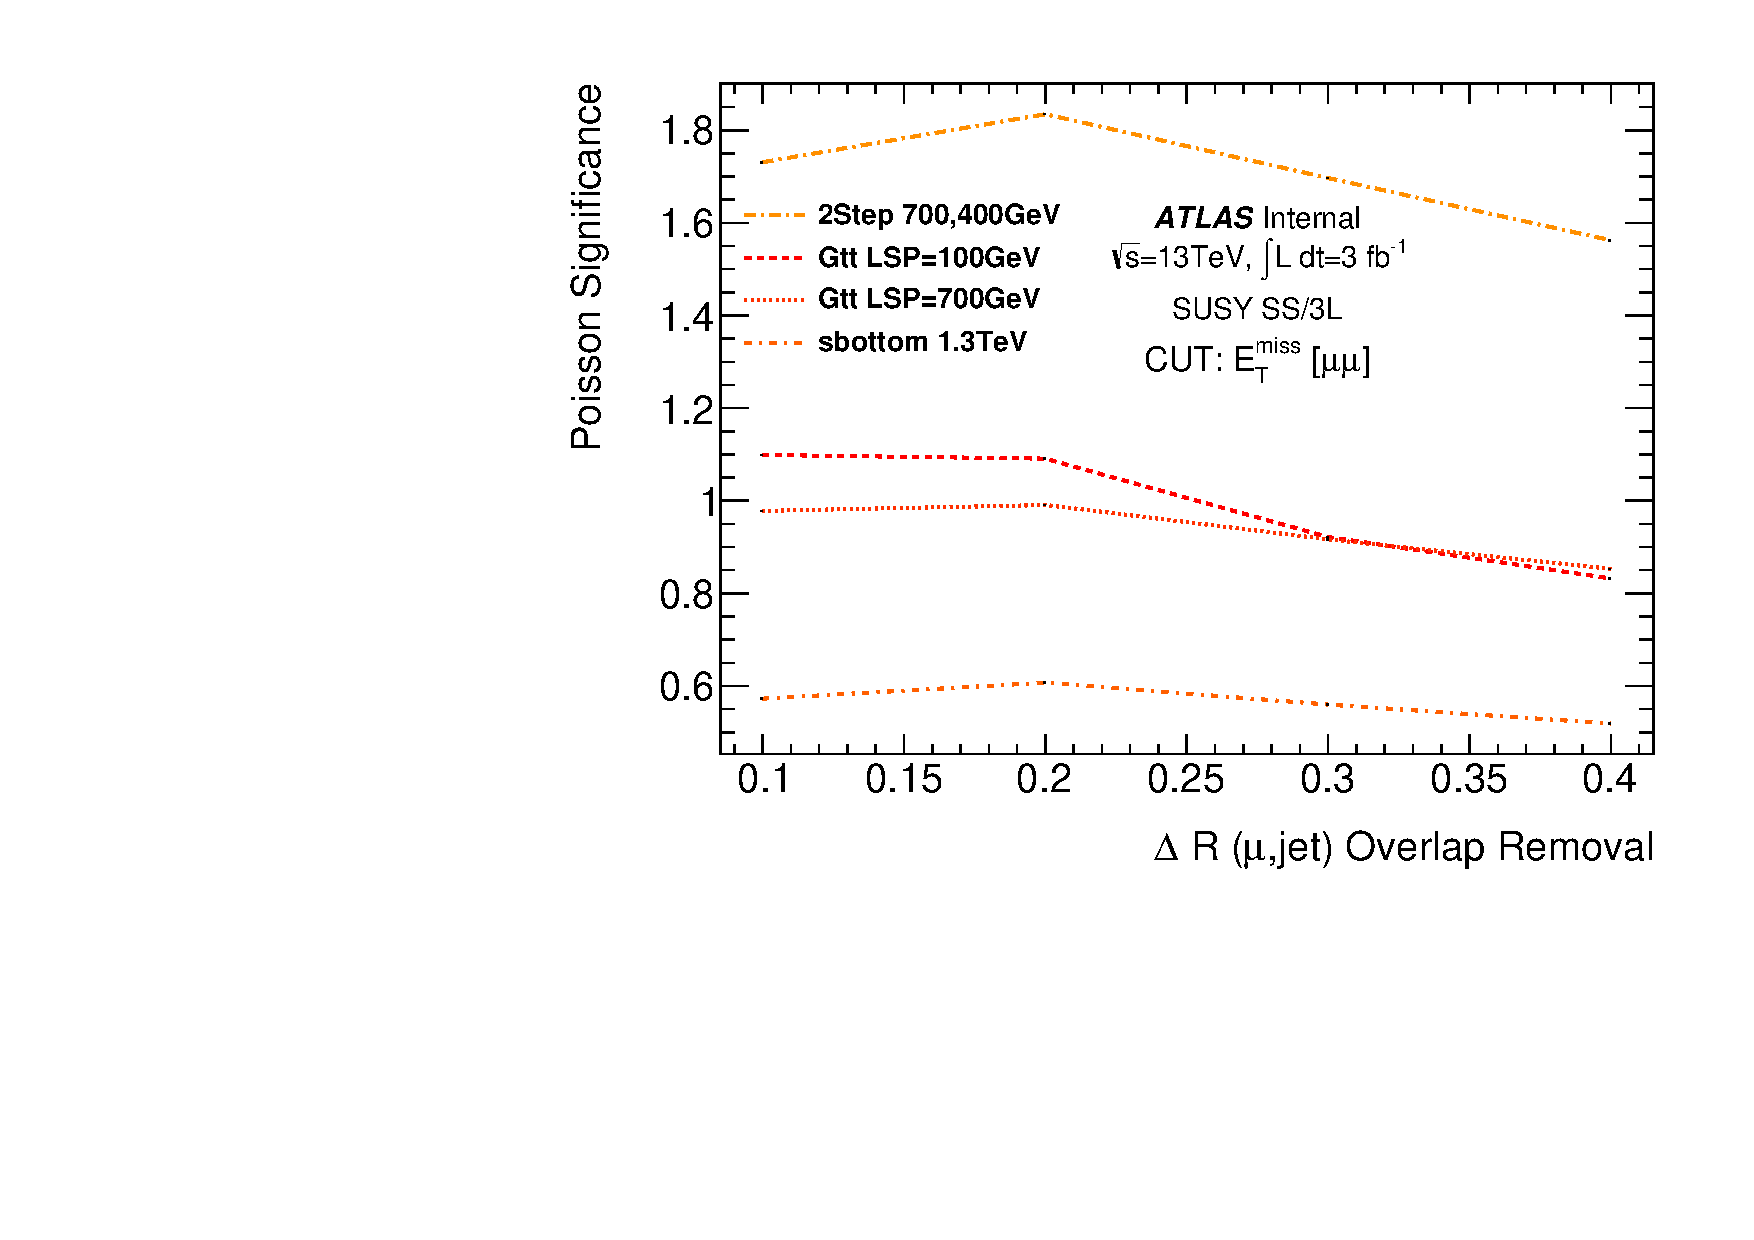
\includegraphics[width=0.45\textwidth]{OVERLAPREMOVAL/plot_significance_mm.pdf} 
%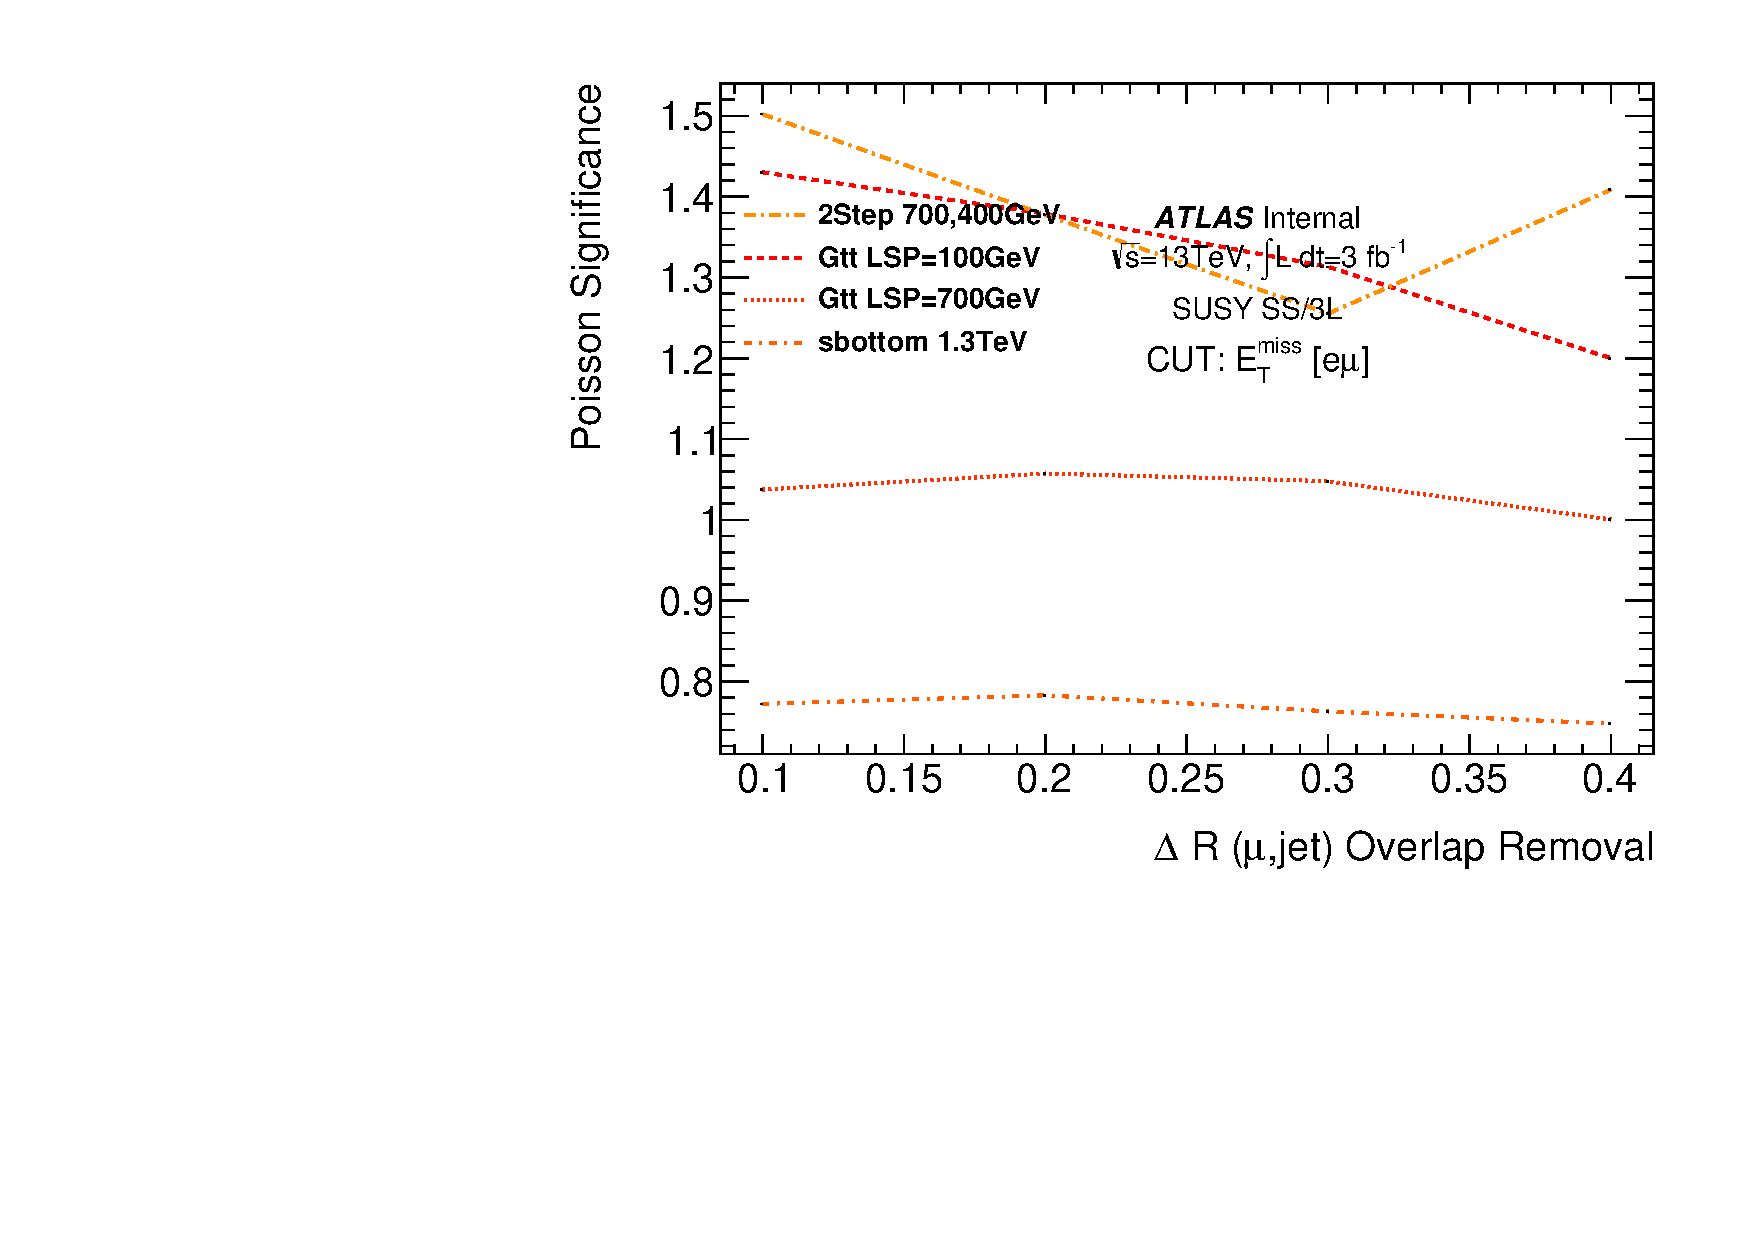
\includegraphics[width=0.45\textwidth]{OVERLAPREMOVAL/plot_significance_em.pdf} 
%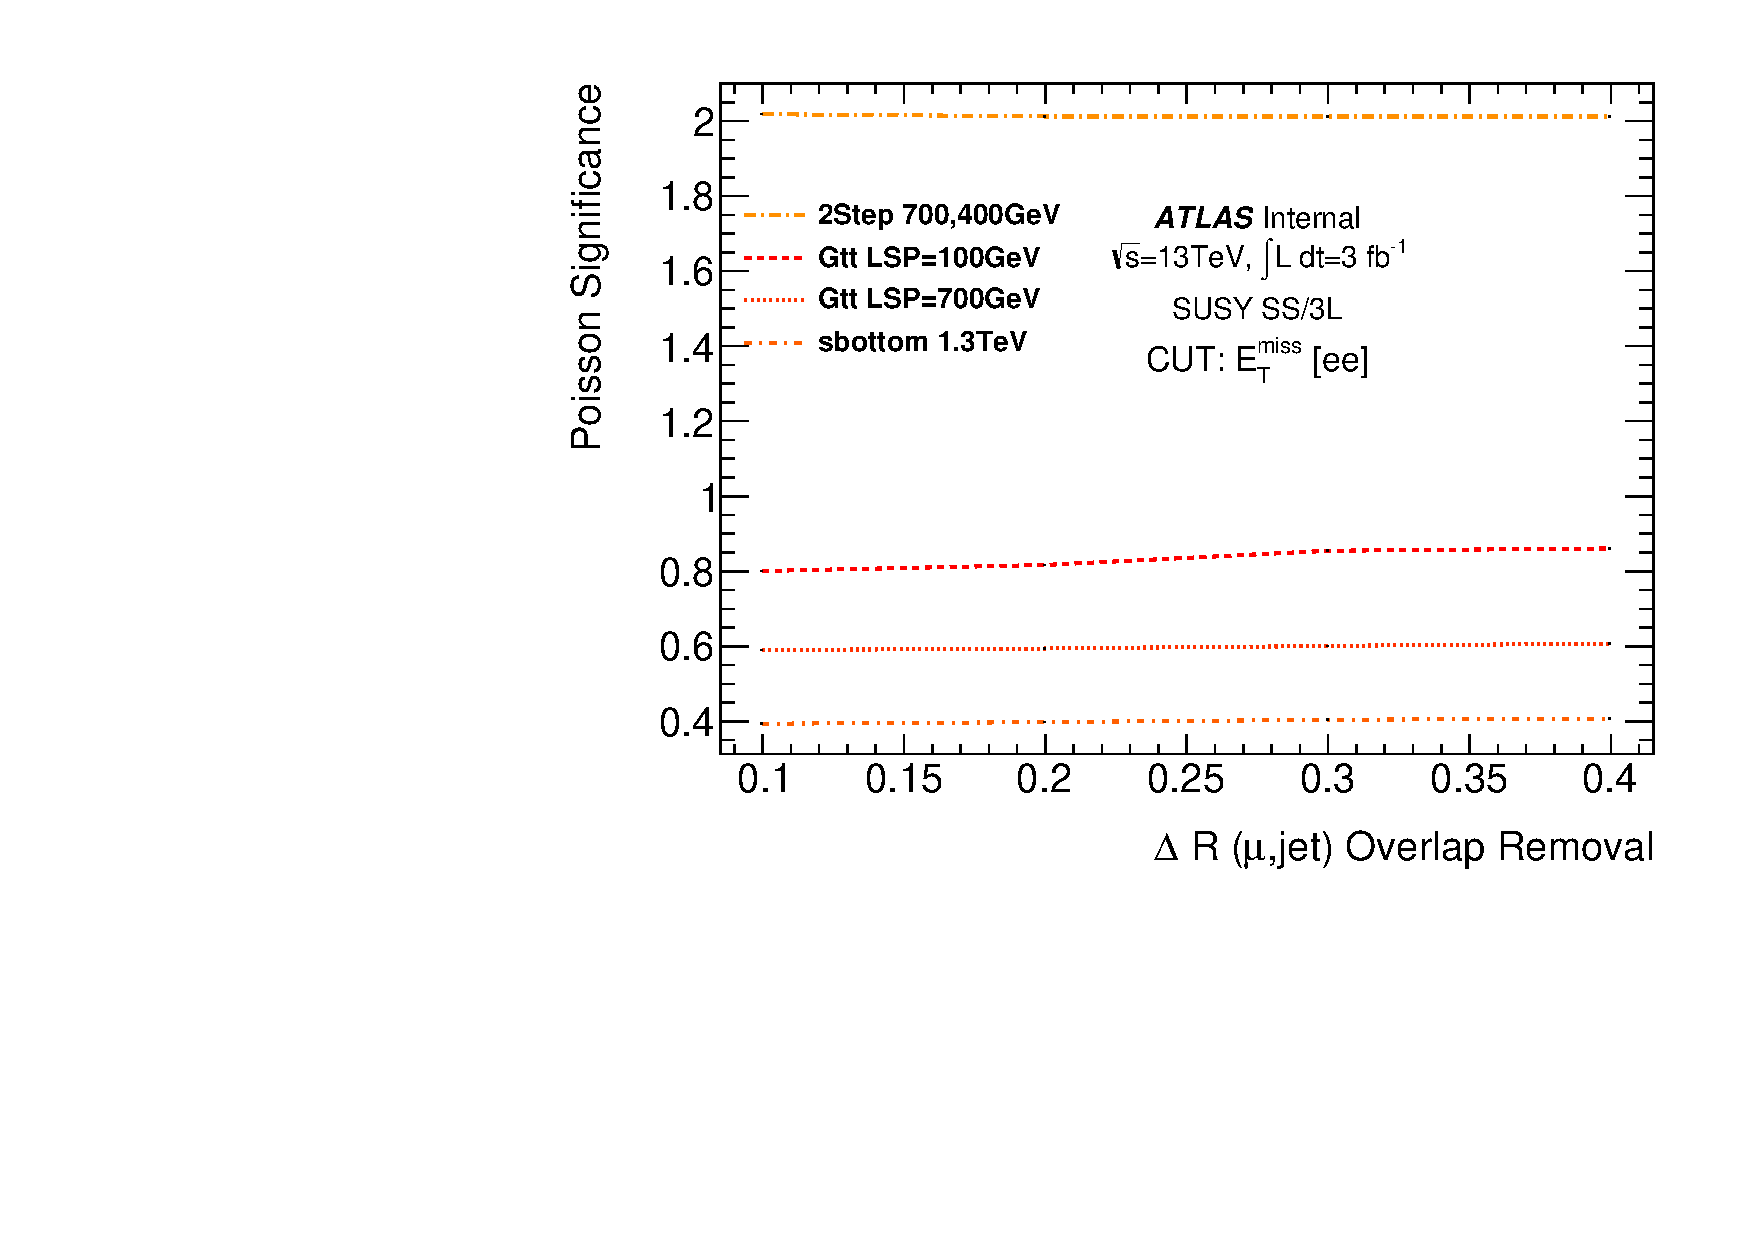
\includegraphics[width=0.45\textwidth]{OVERLAPREMOVAL/plot_significance_ee.pdf} 
%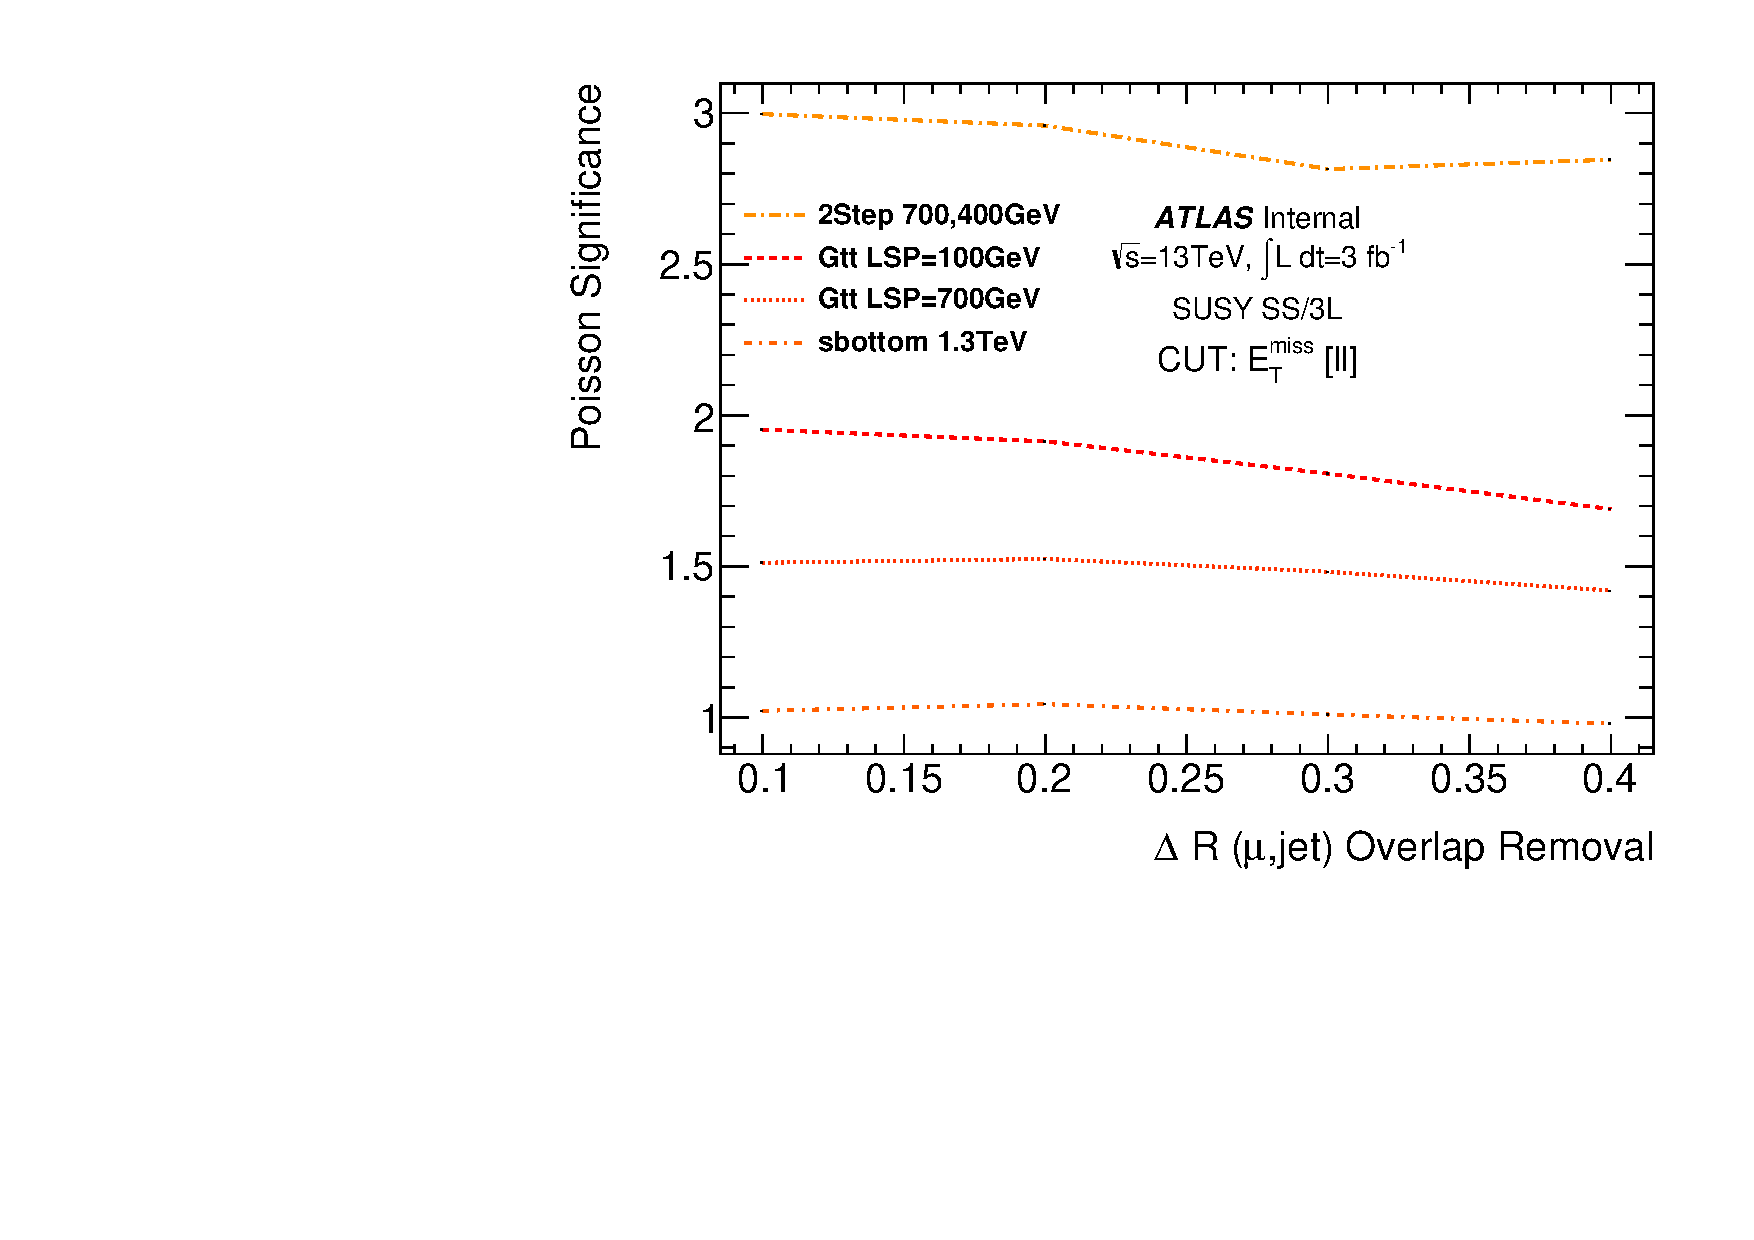
\includegraphics[width=0.45\textwidth]{OVERLAPREMOVAL/plot_significance_ll.pdf} 
%\end{center}
%\vspace{-0.2cm}
%\caption{Discovery significance for an assumed integrated luminosity of 3~fb$^{-1}$, for different choices of cone separation used for the muon-jet object overlap removal in various signal models. 
%Top figures display the significance for the muon-related channels ($\mu\mu$ and $e\mu$) and bottom figues illustrate the effect on the $ee$ channel as well as the flavour combination.}
%\label{fig:OR_significance}
%\end{figure}
%
%The studies seem to favor a choice of a $\Delta R$ of 0.2.  


\subsection{Missing transverse energy}
\label{sec:objects_met}

The missing transverse energy (\met) is rebuilt using the xAOD container ``MET\_RefFinal'' as input and using the calibrated electron, muon and jet objects 
(and baseline photons according to SUSYTools definitions). 
In this version of the analysis, the track soft term is used for building the \met\ following the defaults in SUSYTools-00-07-17.


\subsection{Lepton truth matching}
\label{sec:truth_matching}

In several studies presented in this document, 
a lepton truth matching strategy is applied to distinguish the lepton originating from prompt decays of gauge boson or SUSY particles 
from non-prompt leptons originating from semileptonic $b$-decays, photon conversions or fakes. 
This strategy largely relies on the information from the {\tt MCTruthClassifier} tool. 
However, the latter does not always allow to properly classify electrons originating from a photon conversion, 
where it is important to fully understand the origin of the photon and its possible proximity to a prompt electron 
(FSR, brehmsstrahlung, which is the main mechanism leading to charge-flip electrons). 
In these cases, we complete this information by a matching within a cone of $\Delta R <0.1$ with truth prompt electrons, 
which are identified as the decays of heavy bosons ($W$, $Z$, $h$) or SUSY particles. 
This is however only possible in MC generators storing intermediate resonances in the event record, 
i.e. notably MC samples in which decay chains are handled by Pythia. 

\FloatBarrier



\section{Event selection}
\label{sec:evtsel}

\subsection{Trigger studies}
\label{sec:trigger}
The trigger strategy for the analysis in Run-2 is similar to the one used in the Run-1 version. There, a combination of \met , 
single-lepton and di-lepton triggers was used for the selection of events in the signal region and control distributions. The triggers were checked consecutively starting with the \met\ trigger, followed by the single lepton trigger and the dilepton triggers, until one of the triggers is passed by the event. Offline cuts on the missing energy and the \pt\ of the triggered objects were applied to ensure to be on the efficiency \textit{plateau} of the corresponding trigger.

For Run-2 the triggers to be used are also missing energy and single- and di-lepton triggers. The lepton trigger menu includes triggers selecting isolated and non-isolated leptons as well as dilepton triggers selecting mixed-flavor lepton events. 
The following triggers have been regarded as important for this analysis and were used for further studies on performance and efficiency:

\begin{itemize}
\item Single-lepton triggers: \texttt{HLT\_mu26, HLT\_mu50, HLT\_mu24\_imedium, HLT\_mu26\_imedium}, 

\texttt{HLT\_e20\_medium, HLT\_e60\_medium, HLT\_e24\_tight\_iloose, HLT\_e26\_tight\_iloose}

\item Di-lepton triggers: \texttt{HLT\_2m10, HLT\_2mu14, HLT\_2e12\_loose\_L12EM10VH, HLT\_2e17\_loose, HLT\_e17\_loose\_mu14}

\item Multi-lepton triggers \texttt{HLT\_3m6, HLT\_e12\_loose\_2mu10}

\item \met\ triggers: \texttt{HLT\_xe60, HLT\_xe70, HLT\_xe100, HLT\_xe100\_cell}

\end{itemize}

The performance of these triggers has been investigated by running the analysis 
on dedicated $Z \rightarrow \mu \mu$, $Z \rightarrow ee$ and $t \bar{t}$ Monte 
Carlo samples with several trigger applications.
For each object triggered, an offline cut on the object \pt\ or the \met\ is applied to ensure the full efficiency of the trigger in the selected event. A geometrical $\Delta R$ matching between the lepton triggers fired and the signal leptons reconstructed in each event is applied in order to confirm that the according trigger was activated by one of the signal leptons found in the analysis. 


\subsubsection{Monte Carlo samples and software framework}

The trigger studies were performed with the latest available releases of the ATLAS software framework and the latest Monte Carlo productions. The analysis code was setup with the \texttt{AnalysisBase} framework (2.3.8 branch for rel.20 ATLAS software). The object selection was done by using the \texttt{SUSYTools-00-06-03} package which provides the current recommendations for selection of signal and baseline objetcs. 

The Monte Carlo samples used for these studies are validation samples produced with the 20.1.4.3 MC15 ATLAS software release (no pileup). 

\begin{itemize}

\item $t \bar{t}$ sample: 

\texttt{valid3.110401.PowhegPythia\_P2012\_ttbar\_nonallhad.recon.AOD.e3099\_s2578\_r6540}

\item $Z \rightarrow \mu \mu$ sample:  

\texttt{valid3.167826.Sherpa\_CT10\_ZmumuMassiveCBPt280\_500\_CVetoBVeto.recon.AOD.e3099\_s2578\_r6540}

\item $Z \rightarrow e e$ sample: 

\texttt{valid3.147406.PowhegPythia8\_AZNLO\_Zee.recon.AOD.e3099\_s2578\_r6540}

\end{itemize}

\subsubsection{Total event yields}

The total event yields for the test MC samples and different trigger configurations was measured. The yields are shown in Fig.~\ref{fig:events} for the $t \bar{t}$ Monte Carlo sample and for the $Z \rightarrow \mu \mu$, $Z \rightarrow ee$ samples respectively. The trigger performance is as expected: while for $Z \rightarrow \mu \mu$ Monte Carlo, the muon triggers select most of the events, for $Z \rightarrow ee$ the electron triggers do. For $t \bar{t}$ Monte Carlo, the muon- and electron triggers have similar selection rates, and most events are selected by applying \met\ triggers.

\begin{figure}[htb!]
\centering
\subfigure{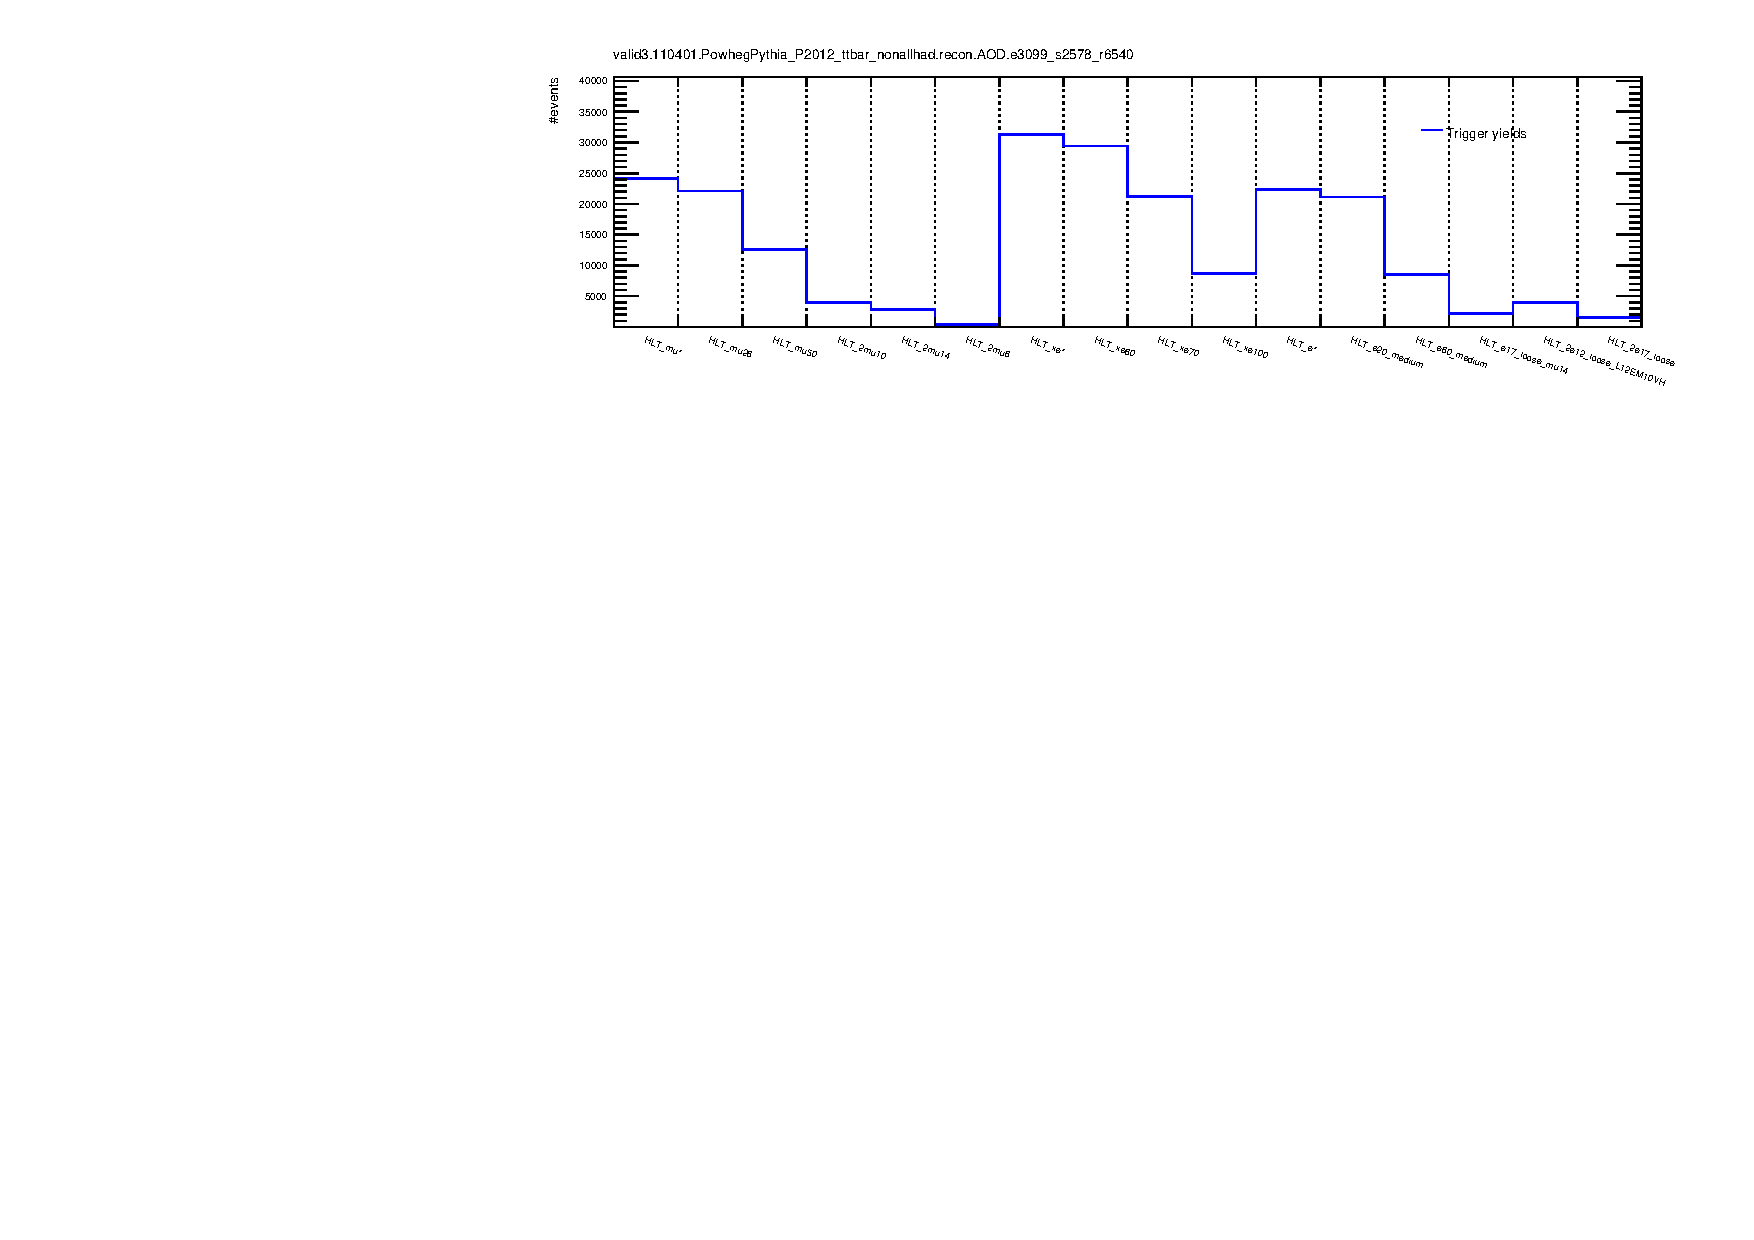
\includegraphics[width=1.\textwidth]{TRIGGER/Events_ttbar}}
\subfigure{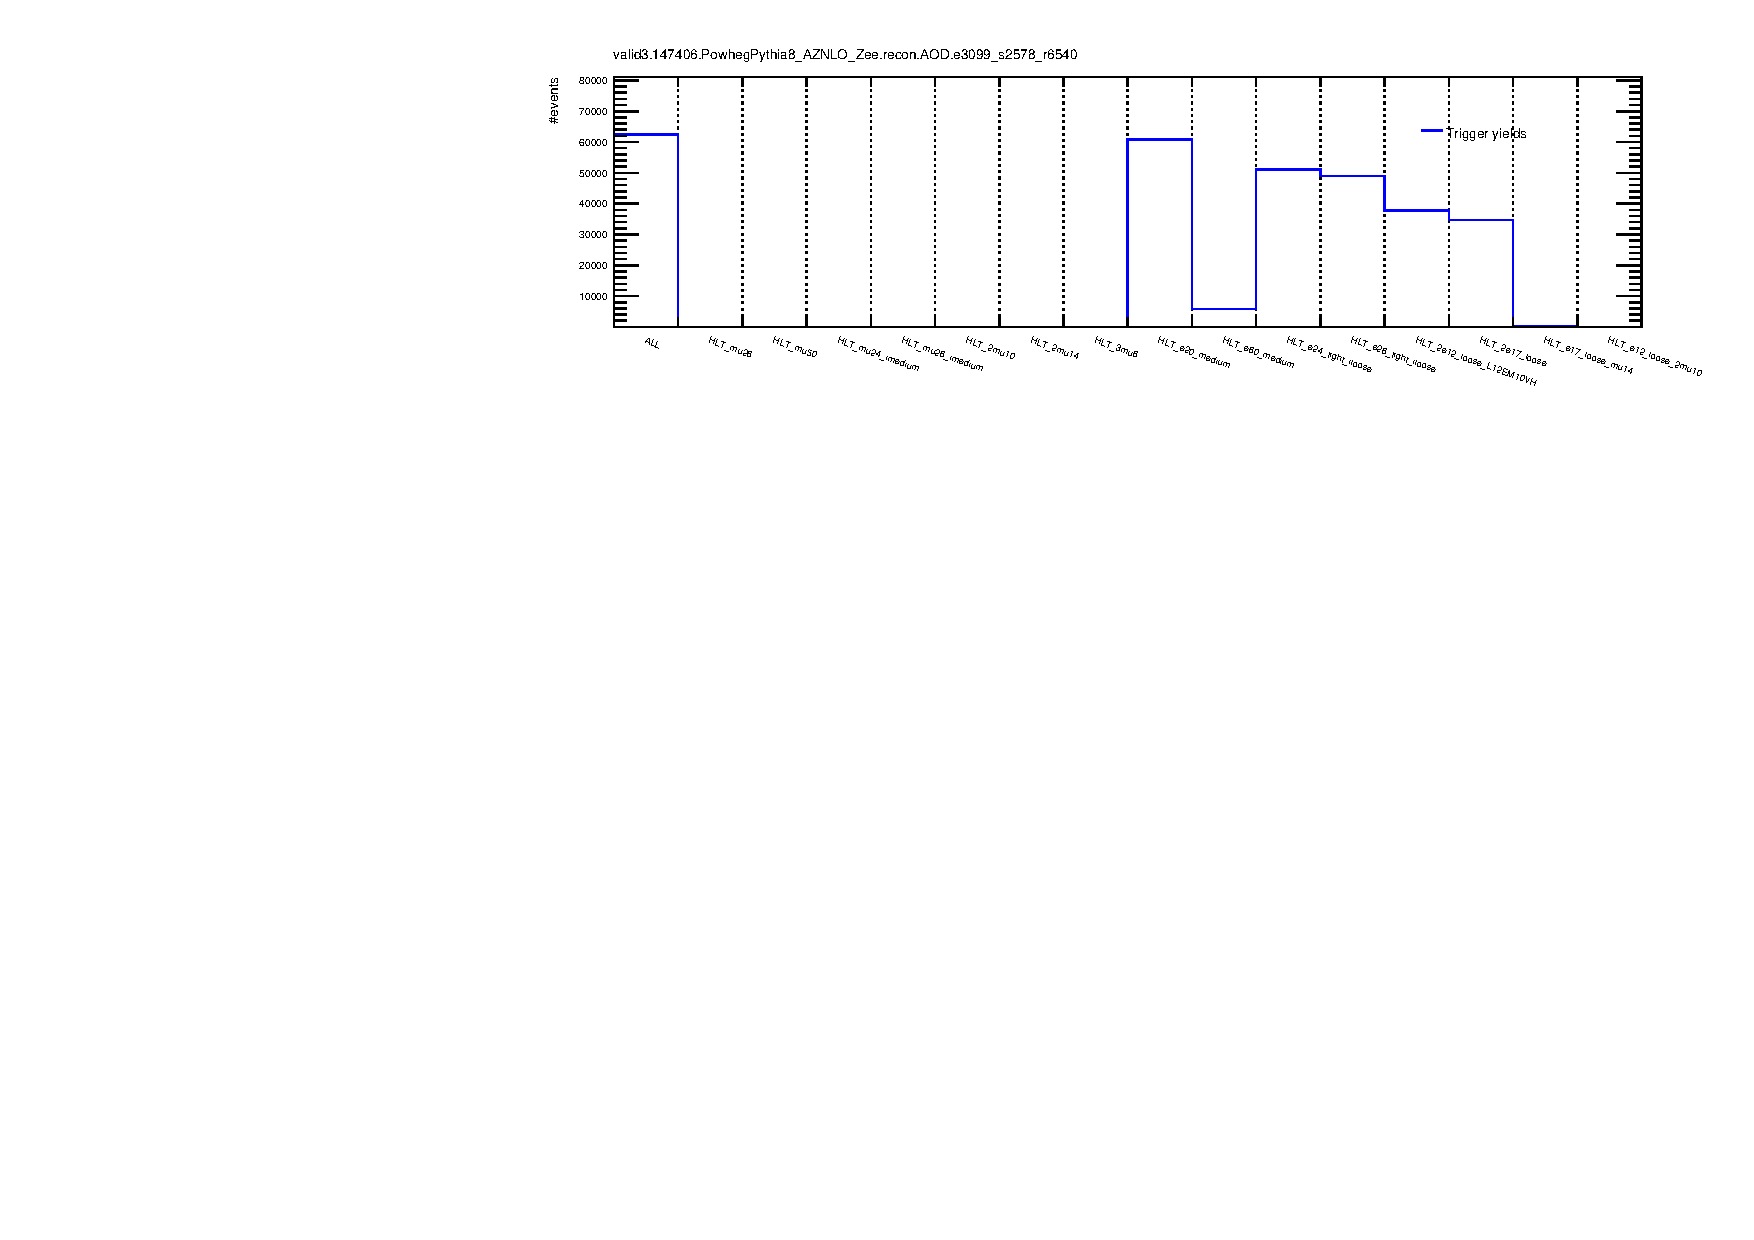
\includegraphics[width=1.\textwidth]{TRIGGER/Events_Zee}}
\subfigure{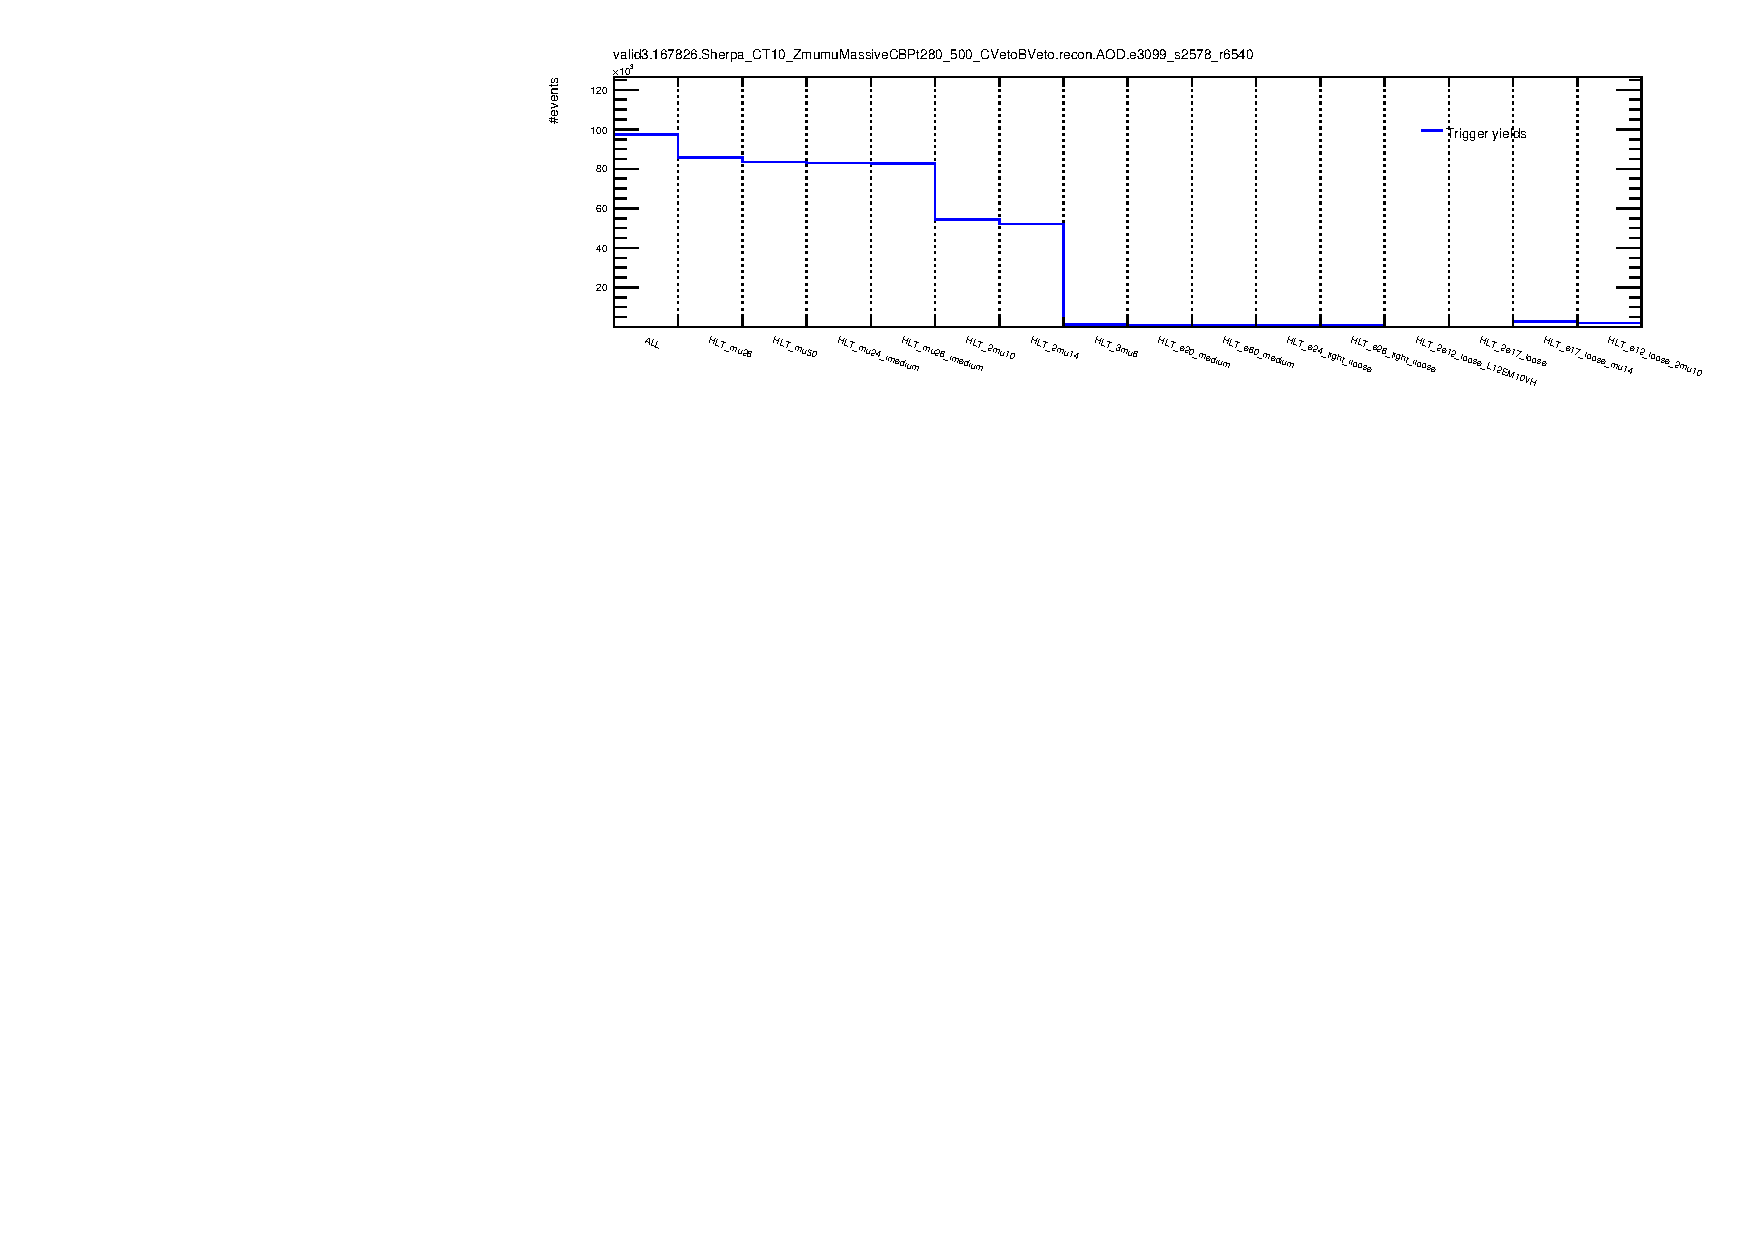
\includegraphics[width=1.\textwidth]{TRIGGER/Events_Zmumu}}
\caption{Total event yields for the $t \bar{t}$ sample (top) and for the $Z \rightarrow \mu \mu$ (middle), $Z \rightarrow ee$ (bottom) samples. On the x-axis the different triggers (or trigger configurations) are shown.}
\label{fig:events}
\end{figure}

\subsubsection{Efficiencies}

The trigger efficiency in Monte Carlo can be obtained by dividing the number of triggered events by the total number of events. The efficiencies have been calculated separately for single-lepton, dilepton triggers and for \met\ triggers. The results for some examples are shown in Fig.~\ref{fig:eff_singlelepton} for single lepton triggers and for dilepton and \met\ triggers on Fig.~\ref{fig:eff_dilepton_met}. Further efficiency plots can be found in Appendix~\ref{app_trigger}. The turn-on curves for the single-lepton and dilepton triggers show the expected evolution. The efficiency at the trigger plateau is between 95\% - 98\% for single-lepton and around 90\% for dilepton triggers. For the \met\ trigger, the turn-on is slower with respect to the quoted online threshold. It reaches its efficiency plateau if \met\ $>$ 250 GeV and the efficiency value in plateau is around 80\%.  

\begin{figure}[htb!]
\centering
\subfigure{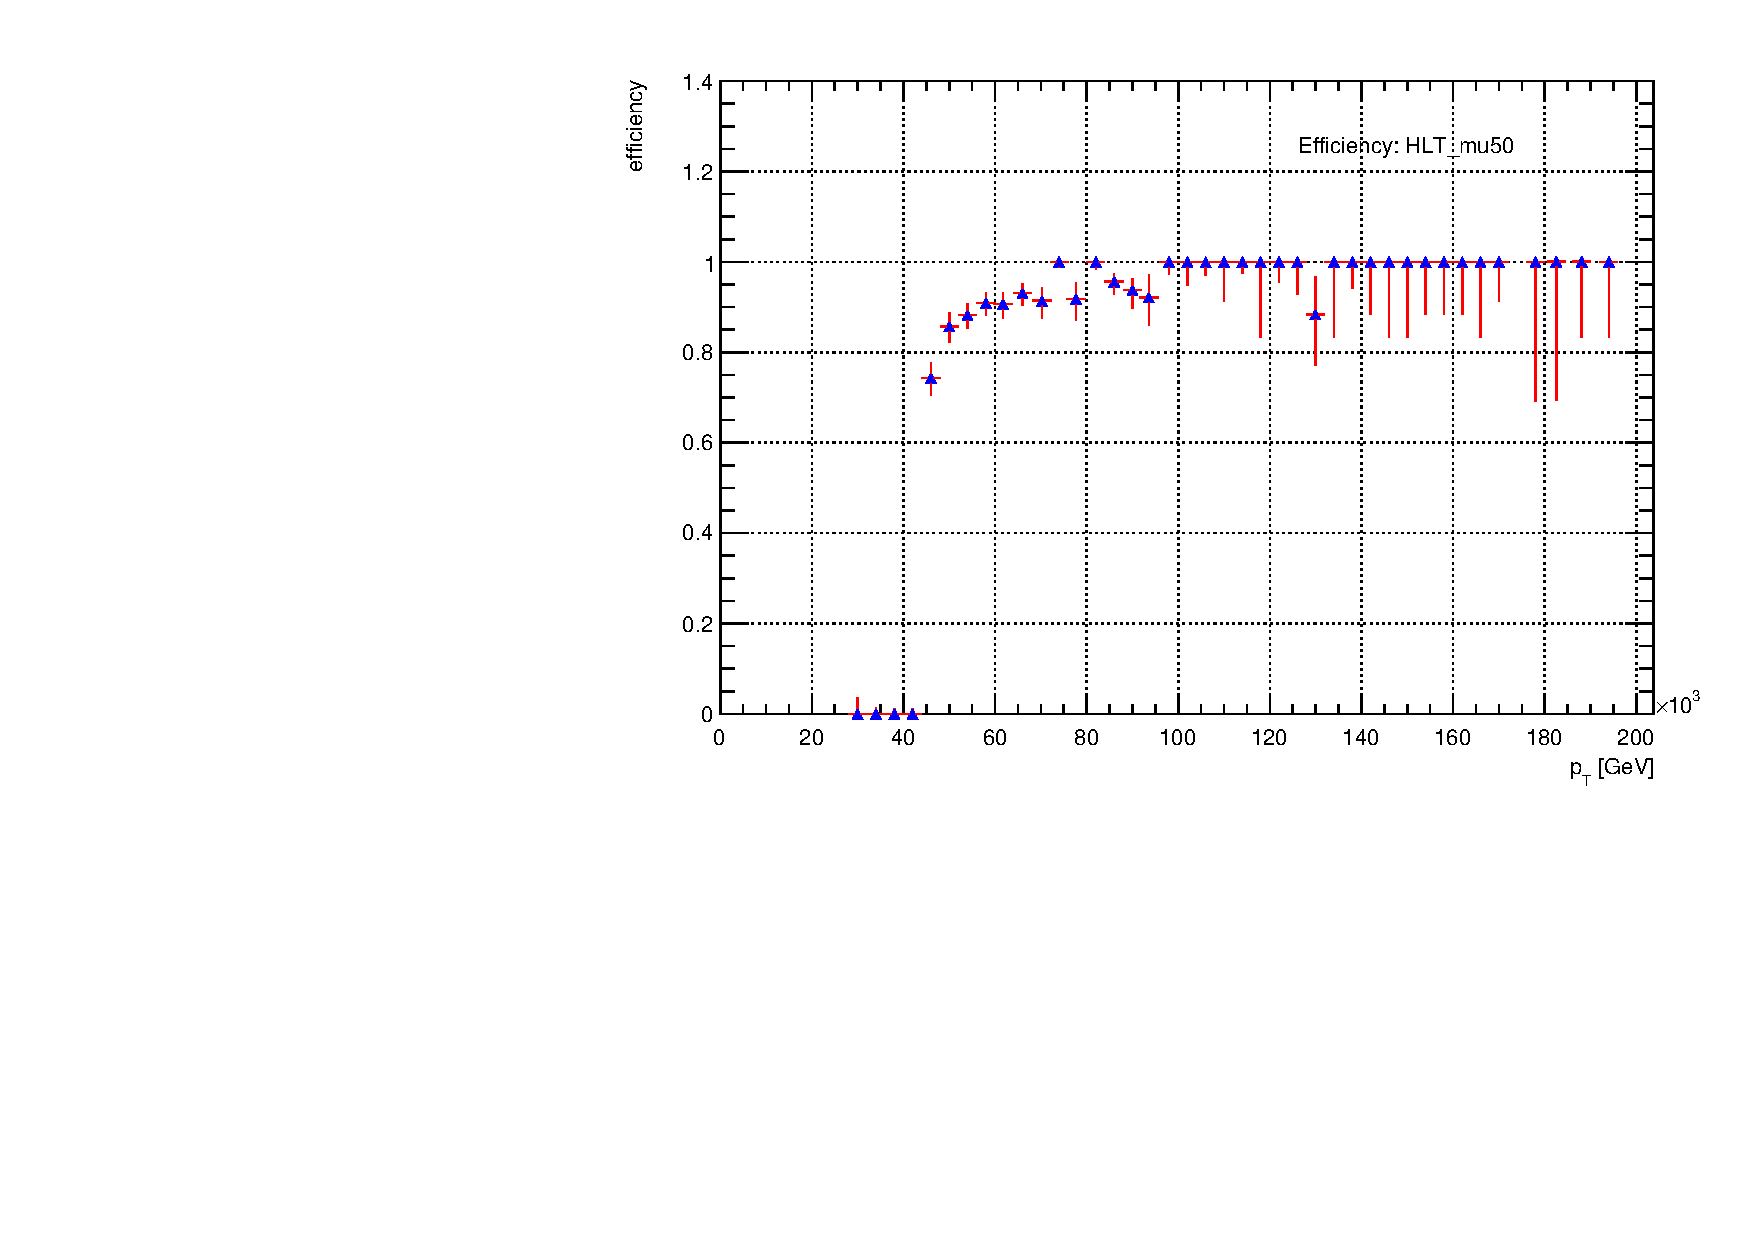
\includegraphics[width=0.48\textwidth]{TRIGGER/Eff_HLT_mu50}}
\subfigure{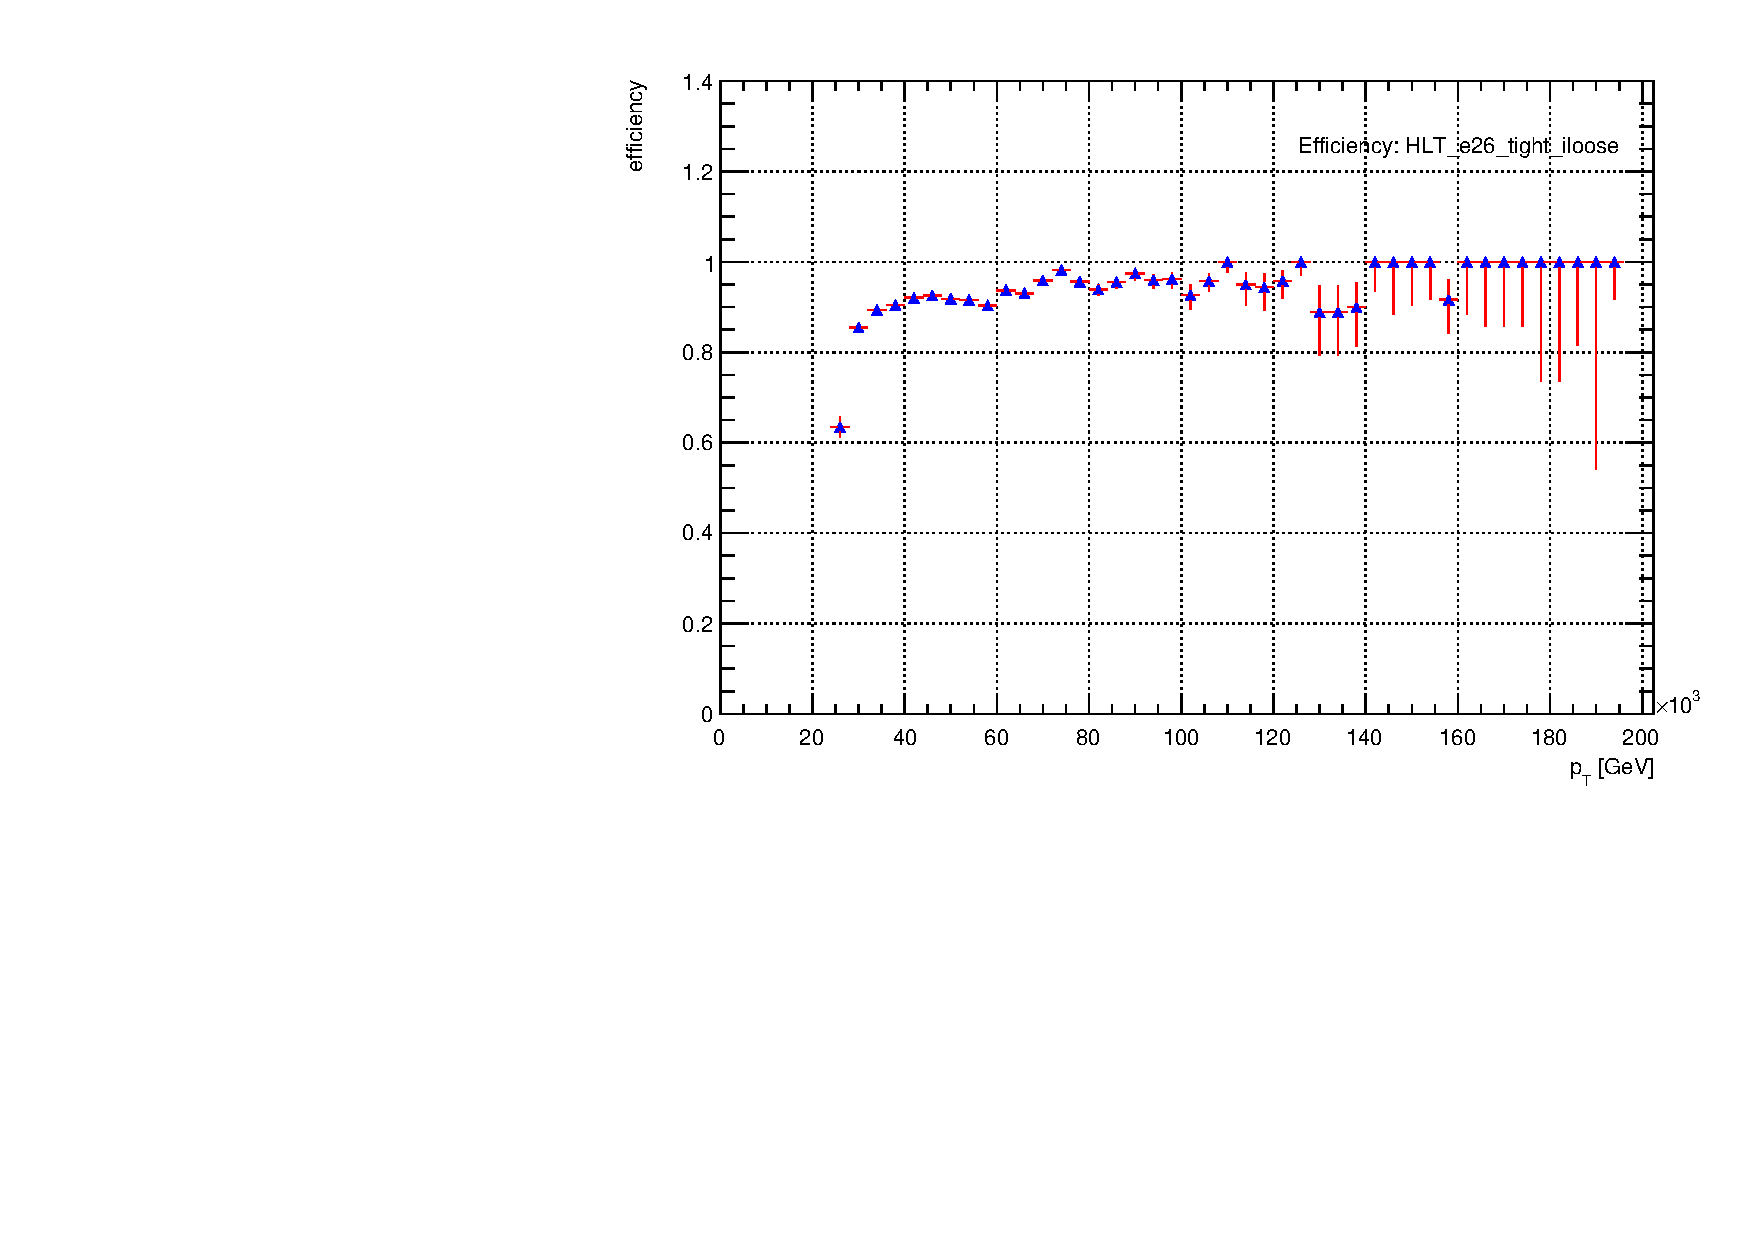
\includegraphics[width=0.48\textwidth]{TRIGGER/Eff_HLT_e26_tight_iloose}}
\caption{Trigger efficiencies for \texttt{HLT\_mu50} and \texttt{HLT\_e26\_tight\_iloose} versus \pt\ of the leading lepton. 
%The turn-on curves of the triggers are close to the expected threshold of the online efficiency. The efficiency on the trigger plateau is around 95\%.
}
\label{fig:eff_singlelepton}
\end{figure}

\begin{figure}[htb!]
\centering
\subfigure{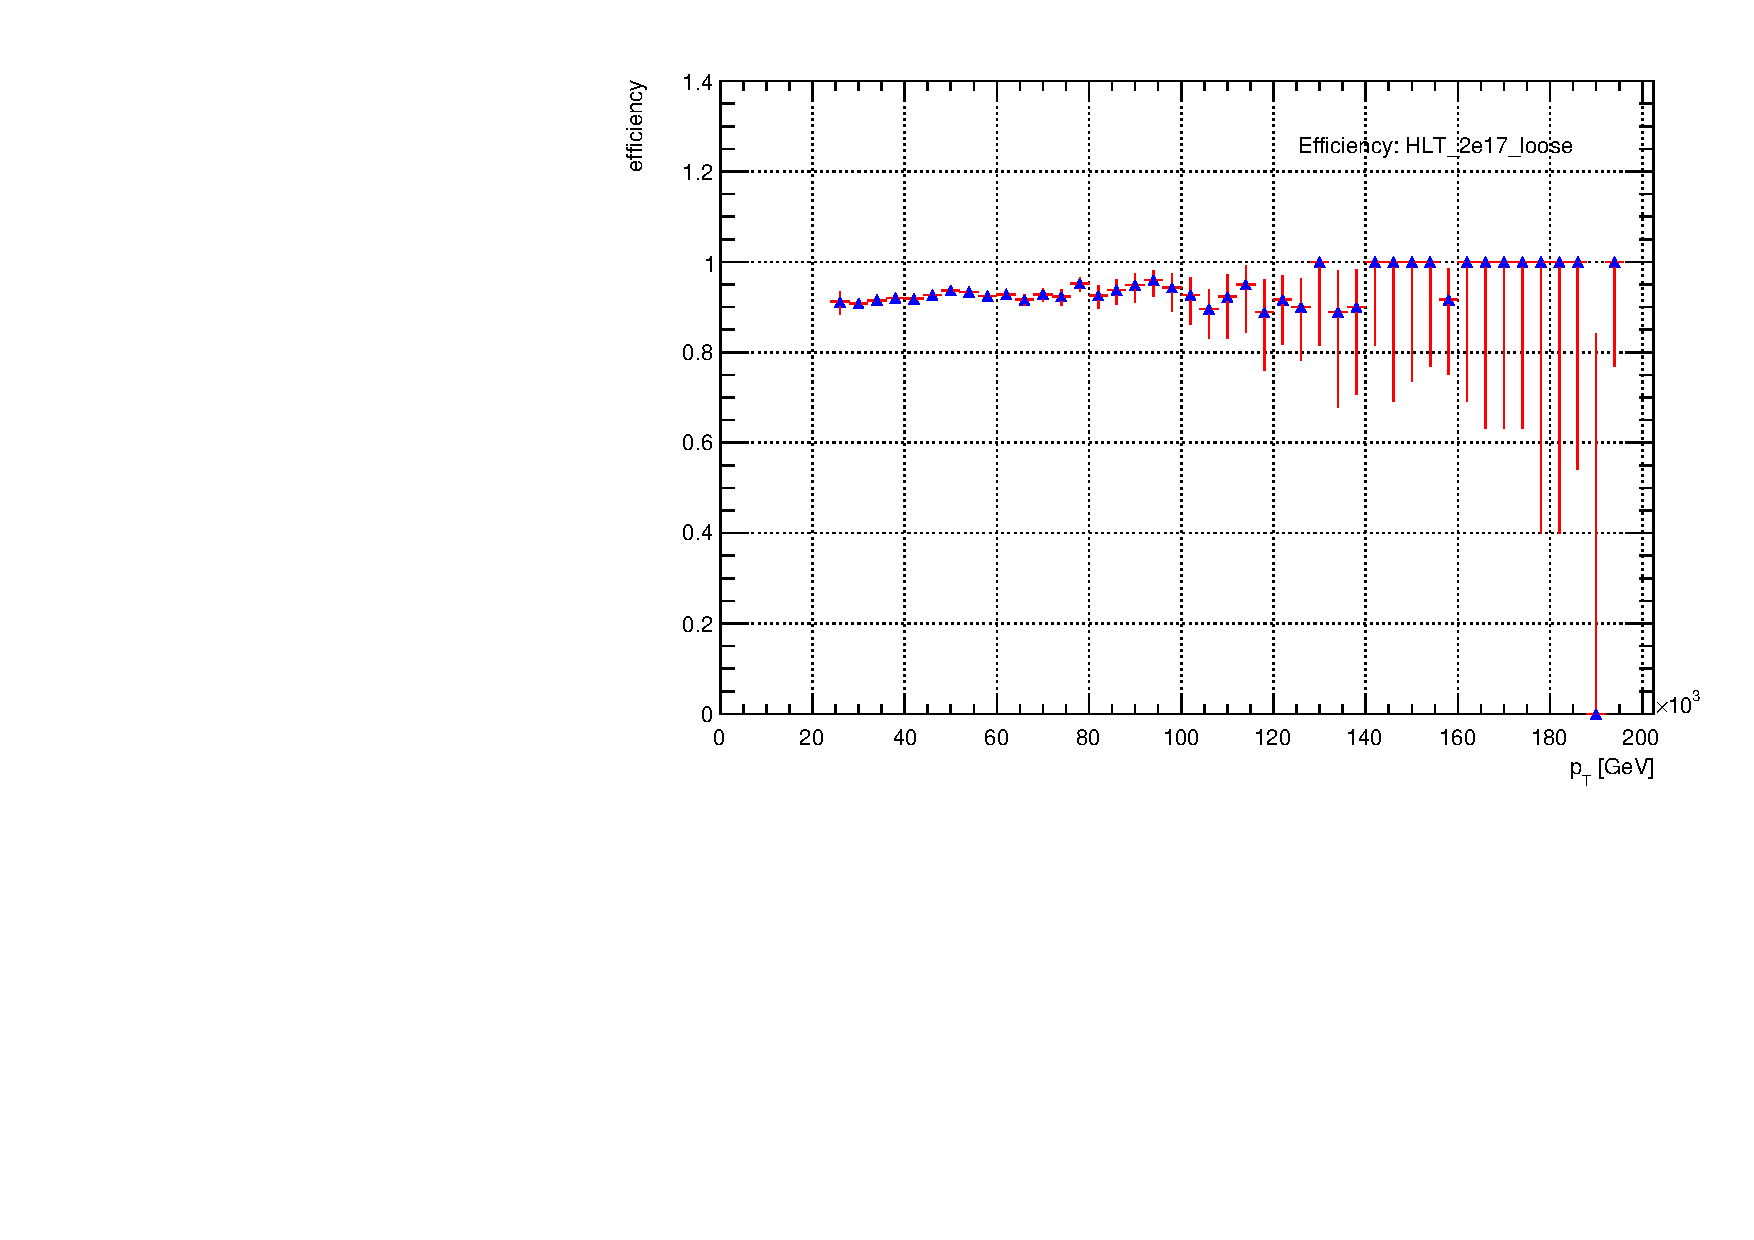
\includegraphics[width=0.48\textwidth]{TRIGGER/Eff_HLT_2e17_loose}}
\subfigure{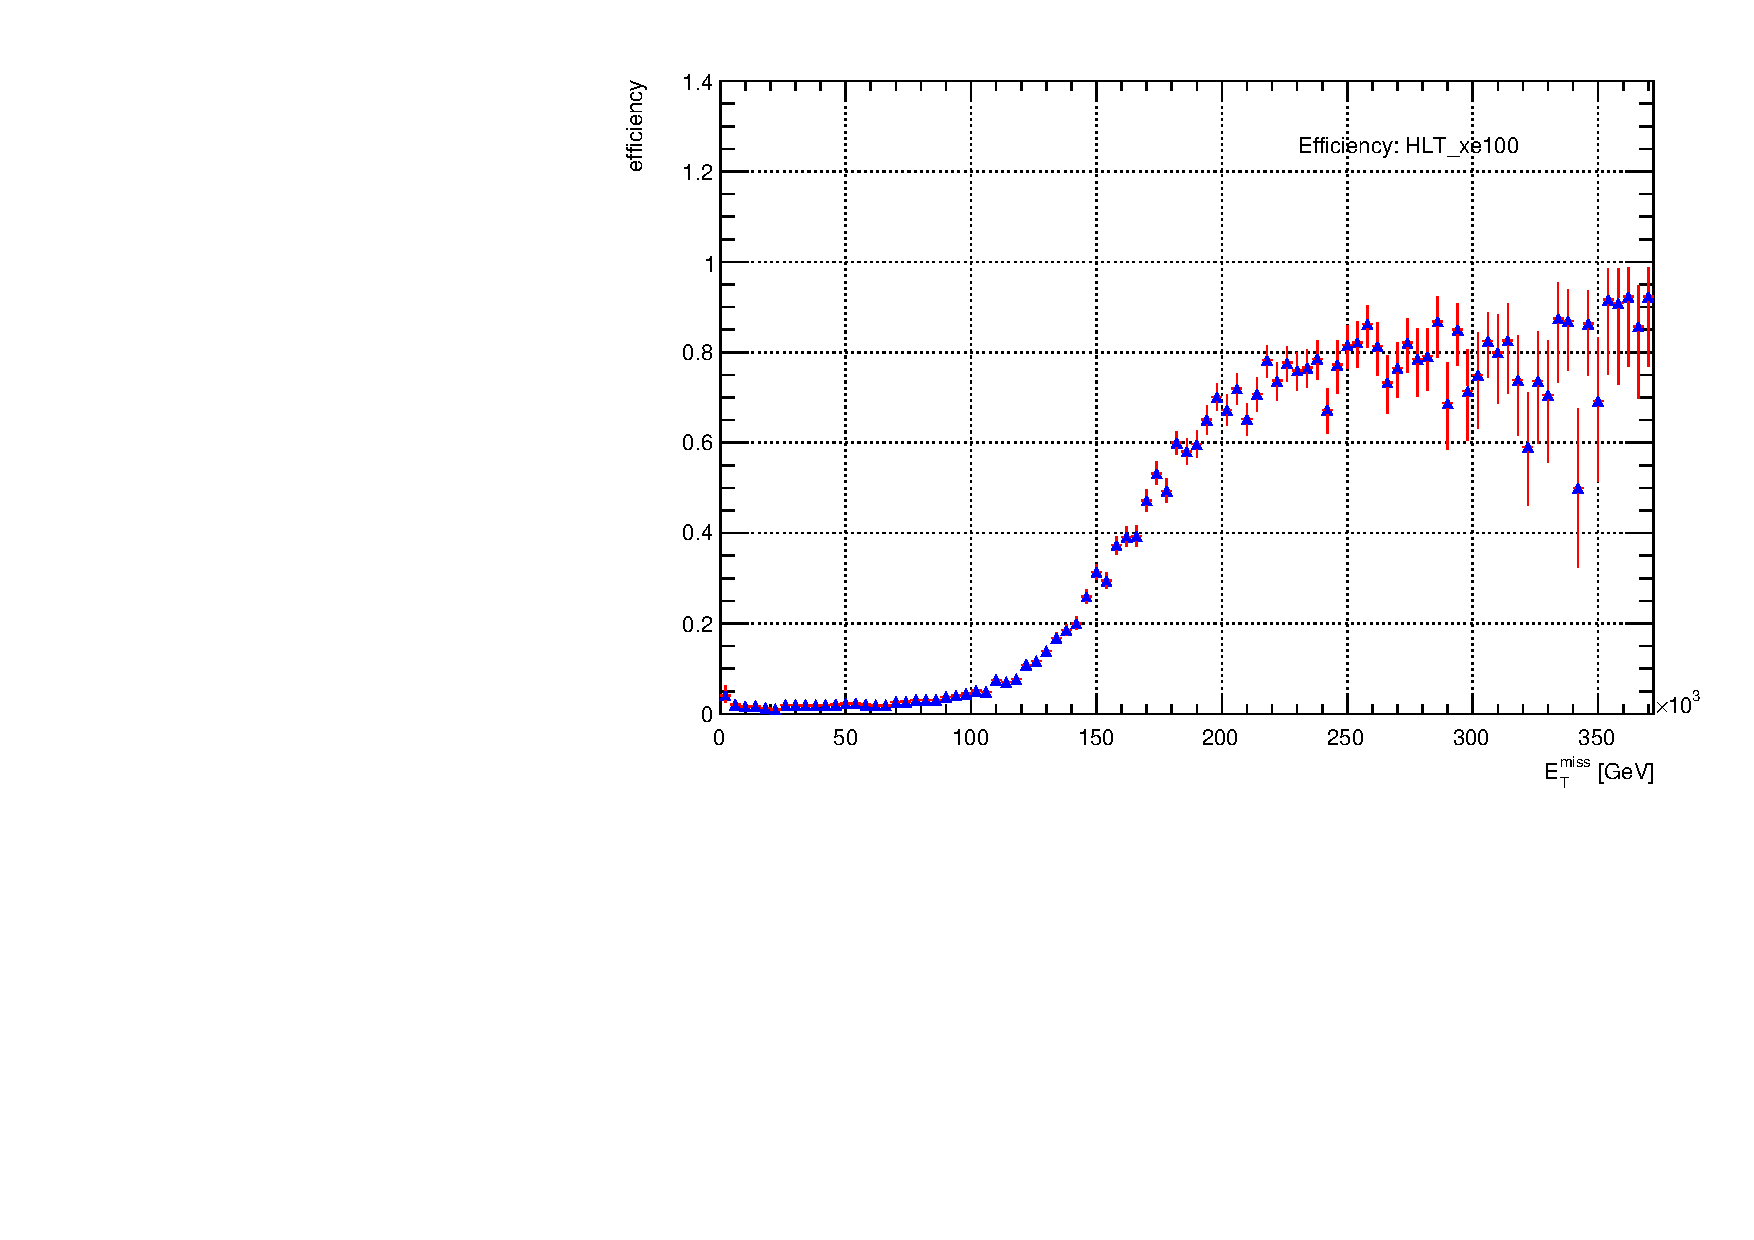
\includegraphics[width=0.48\textwidth]{TRIGGER/Eff_HLT_xe100}}
\caption{Trigger efficiencies for \texttt{HLT\_2e17\_loose} (left) and \texttt{HLT\_xe100} (right). The efficiency for the dilepton trigger is plotted against the \pt\ of the leading electron while the efficiency of the \met\ trigger is plotted against the corrected missing energy value. %Both triggers show the expected performance on the efficiency plateau. The dilepton trigger reaches an efficiency of around 90\%. For the \met\  trigger, the turn-on is slower. At the plateau it reaches also an efficiency of around 90\%.
}
\label{fig:eff_dilepton_met}
\end{figure}



\subsection{Event pre-selection}
\label{sec:presel}

%A few general selection criteria based on data quality, detector quality flags are the following:
\par A sample of two same-sign or three leptons is selected applying the following criteria:
\begin{itemize}
%\item{ \textbf{GRL}: The used GoodRunsList, providing a total
%    luminosity of $\lumi$~\ifb, was \newline
%\small{\texttt{data12\_8TeV.periodAllYear\_DetStatus-v58-pro14-01\_DQDefects-00-00-33\_PHYS\_StandardGRL\_All\_Good.xml}}.}
%\item{ \textbf{Trigger}: The data have been collected using lepton and \met\ triggers, as described in Section \ref{section:trigger}.}
%\item{ \textbf{LAr and Tile Error}: Impact from the noise bursts and data corruption in the LAr and
% Tile calorimeter is reduced by selecting events without an error from
% the quality checks (larError!=2 and tileError!=2). } 
%\item{ \textbf{Incomplete events}: Incomplete events due to the TTC restart procedure are rejected.}

%\item{ \textbf{Fake \met\ Veto}: Events with fake \met\ due to jets
%    pointing to dead TileCal and HEC regions are rejected. This is
%    achieved by vetoing events with at least one
%    jet~\footnote{Anti-k$_{\rm T}$ jets with $R=0.4$ before
%      electron-jet overlap removal are considered for the veto. } satisfying:
%    \newline 
%$\pt > 40\,\GeV\ \&\&\ C_{jet}  > 0.05\ \&\&\ \Delta\phi (\met,jet) <
%    0.3$ \newline where  $C_{jet}$ is the estimated correction factor  
%    for the energy losses estimated using the jet profile. The veto is applied
%    to all events in data and simulation.}
    
\item{ \textbf{Jet Cleaning}: Events are required to pass the
  {\tt{VeryLooseBad}} set of cleaning requirements recommended by Jet-\met\ group \cite{jetcctwiki} 
  and implemented in the {\tt{JetCleaningTool}}. 
An event is rejected if at least one of the pre-selected jets (thus
after jet-electron overlap removal) fails the jet quality criteria. 
The cleaning requirements are intended to remove events where significant energy was deposited in
  the calorimeters due to instrumental effects such as cosmic rays,
  beam-induced (non-collision) particles, and noise. } 
  
\item{ \textbf{Primary Vertex}: events are required to have a primary vertex, that is, one of the reconstructed vertices
   must be labeled as {\tt{xAOD::VxType::PriVtx}}. No additional requirements on the number of tracks in the 
   vertex should be applied as recommended by the Tracking CP group~\cite{vertex_twiki}.
}

\item{ \textbf{Bad Muon Veto}:  Events containing at least one pre-selected muon satisfying $\sigma(q/p)/|q/p| >$ 0.2 before the overlap removal are rejected.}

\item{ \textbf{Cosmic Muon Veto}: Events containing a cosmic muon candidate are rejected. Cosmic muon candidates are selected among pre-selected muons, if they fail the requirements $|z_0| <$ 1.0\,mm and $|d_0| <$ 0.2\,mm, where the longitudinal and transverse impact paramaters $z_0$ and $d_0$ are calculated with respect to the primary vertex.}

\item{ \textbf{At least two leptons}: Events are required to contain
    at least two signal leptons (see Section~\ref{sec:objects} and
    Table \ref{tab:lepdef}) with $p_{\mathrm{T}}
    > 20\,\GeV$ and $p_{\mathrm{T}} > 15\,\GeV$ for the leading and subleading lepton, respectively. 
    If the lepton contains a third lepton with $p_{\mathrm{T}} > 15\,\GeV$ the event is regarded as three-lepton
    event otherwise as a two-lepton event. Once the trigger is fully operative in the MC samples, 
    one or two of the three leptons will be 
    matched to the trigger object
    if the event is classified as passing a single or dilepton trigger.
    The data sample obtained is then divided into three channels depending on the flavor of the two 
    leading leptons ($ee$, $\mu\mu$, $e\mu$).}

\item \textbf{Electron-muon overlap}: For any events containing at least one of
  each of a signal electron and muon, the event is vetoed if $\Delta R(e, \mu) < 0.1$.

\item{ \textbf{Same sign}: If the event is a two-lepton event the two leading leptons have to be of 
    same charge (same-sign).}
\item{ \textbf{Z-veto}: If the event is a three-lepton event all possible opposite-charge same-flavor lepton
    combinations are combined to calculate a mass $M_{\ell\ell}$. The event is rejected if one of the calculated mass
    is close to the $Z$-mass, i.e.~$84 < M_{\ell\ell} <  98\,\mathrm{GeV}$.}
\item{ \textbf{Invariant mass}: Events with $M_{\ell\ell} < 12\,\GeV$ are
    rejected to avoid heavy flavor meson resonances. In three-lepton events, the invariant mass $M_{\ell\ell}$ is calculated from the 
    two leading leptons. }
\end{itemize}


The following event variables are also used in the definition of the signal and validation regions in the analysis:

\begin{itemize}
\item The inclusive effective mass \meff~ defined as the scalar sum of
  the signal leptons \pt (see Table~\ref{tab:lepdef}), all signal jets \pt\ (see Table~\ref{tab:jetsdef}) and \met;
\item The transverse mass \mt\ computed from the leading lepton and
\met\ as \newline $\mt = \sqrt{2 \cdot \pt^l \cdot \met \cdot (1 - cos(\Delta \phi(l, \met )))}$;
\end{itemize}


\section{Signal region definition}
\label{sec:sr}
\label{sec:SignalRegDef}

The definitions of the signal regions have been studied to provide an optimal performance for $\sqrt s=13$ TeV collisions and a low integrated luminosity (2-4~\ifb). 
This optimization process was first performed with DC14 MC samples, and was then refined with the more accurate MC15 samples and close-to-final object definitions. 
We chose to categorize the signal regions based on their $b$-jet multiplicity, in continuation of the approach sustained in the Run-1 analysis: 
\begin{itemize}
\item[$\bullet$] Signal region(s) with at least one $b$-jet (``SR1b''): these selections target signal scenarios involving top or bottom quarks, 
mostly related to third-generation squarks, such as the benchmark process $\sbot\sbot^*\to t\bar t\tilde\chi_1^+\tilde\chi_1^-$. 
\item[$\bullet$] Signal region(s) with at least three $b$-jets (``SR3b''): these selections target signal scenarios involving many top or bottom quarks, 
such as the benchmark process $\gluino\gluino\to t\bar tt\bar t\ninoone\ninoone$, 
and with their intrinsically very low background are particularly well suited for scenarios with compressed mass spectra. 
\item[$\bullet$] Signal region(s) with a $b$-jet veto (``SR0b''): these selections allow to increase the sensitivity to signal scenarios without bottom quarks, 
by suppressing most of the top background -- the selections are then dominated by diboson background. 
\end{itemize}
One can notice that there is no dedicated selection for final states with $\ge 2$ $b$-jets: 
it is found to not be particularly useful, as the background is generally dominated by $t\bar t+X$ processes, 
which does not change substantially between $\ge 1$ and $\ge 2$ $b$-jets selections. 
By contrast the difference between $\ge 1$ and $\ge 3$ $b$-jets selections is very important. 

To this first classification we add minimal requirements on the inclusive jet multiplicity: 
\begin{center}
\begin{tabular}{c|c|c|c|c}
Signal region(s) & \multicolumn{2}{c|}{SR0b} & SR1b & SR3b\\\hline
Jets req. & $\ge 3$ ($p_T>50$~GeV) & $\ge 5$ ($p_T>50$~GeV) & $\ge 4$ ($p_T>50$~GeV) & $-$\\
\end{tabular}
\end{center}
As one can see, the SR0b selections were subdivided into two overlapping selections ($\ge 3$ or $\ge 5$ jets, 
also denoted as SR0b5j and SR0b3j) to cover various signal scenarios that lead to differently jet-enriched final states. 
The optimal minimal number of jets and the jet $p_T$ thresholds were defined as part of the DC14-based optimization, through a (\meff, \met, \#jets, jet $p_T$) scan similar to the one described below 
and focused on the few benchmark signal scenarios that were produced for DC14 studies. Only the $\pt$ threshold for SR0b3j was raised from 40 to 50~GeV for homogenization among the SRs since this change had very small impact in the sensitivity.

All these selections are inclusive in terms of leptons (``at least two same-sign leptons''), 
it was found that for these early results no substantial gain would be achieved by considering trilepton final states separately (as was done in the Run-1 analysis) except for SR0b3j, where a $\geq$3 lepton requirement was found to improve the sensitivity to slepton-mediated signals ($\gluino\to q\bar{q}(\ell\ell/\ell\nu)\ninoone$).

To complete the definition of the signal regions, we added requirements on the effective mass \meff{} and missing transverse momentum \met. 
We rely only on these two discriminant variables, well suited for generic SUSY searches, 
as one of the analysis strengths is to be sensitive to a broad range of BSM scenarios and we do not want to overtune it to a restricted set of benchmarks. 

\subsection{Optimization procedure and results}

The optimization of the signal region definitions was carried on with the MC15 samples. % (resp. the 50/25 ns configuration for background/signal). 
We scanned the $(\meff,\met)$ plane for the four selections detailed above, 
looking at the impact of the cuts on various signal benchmarks. 
We used as figure of merit the signal discovery significance (Zn), calculated with {\tt RooStats::NumberCountingUtils::BinominalObsZ} 
assuming an overall $40\%$ systematic uncertainty on the background prediction (as a compromise to the 50\% expected uncertainty on the fake-lepton background and 30\% on the prompt-lepton background). 
We discarded the cut configurations where the background projection was too imprecise, due to limited MC statistics; 
more precisely when the statistical error on the projected background exceeded $30\%$. 
We also focused on signal benchmarks that would provide at least 2 signal events for the considered luminosity. 

Figure~\ref{fig:OptimScan} shows as an example the $(\meff, \met)$ planes for two different signal regions and models.
The resulting maximum discovery significance across the signal grids and the corresponding $(\meff,\met)$ configurations 
are shown in Figure~\ref{fig:OptimSig1} for SR1b, SR3b and SR0b5j. As shown, with 2~\ifb\ of data we can have sensitivity beyond the existing Run-1 limits in some of the models. Note that the Run-1 limits shown in the figures correspond to the best ATLAS limit, not necessarily obtained by the SS/3L analysis.

\begin{figure}[!htb]
\centering
  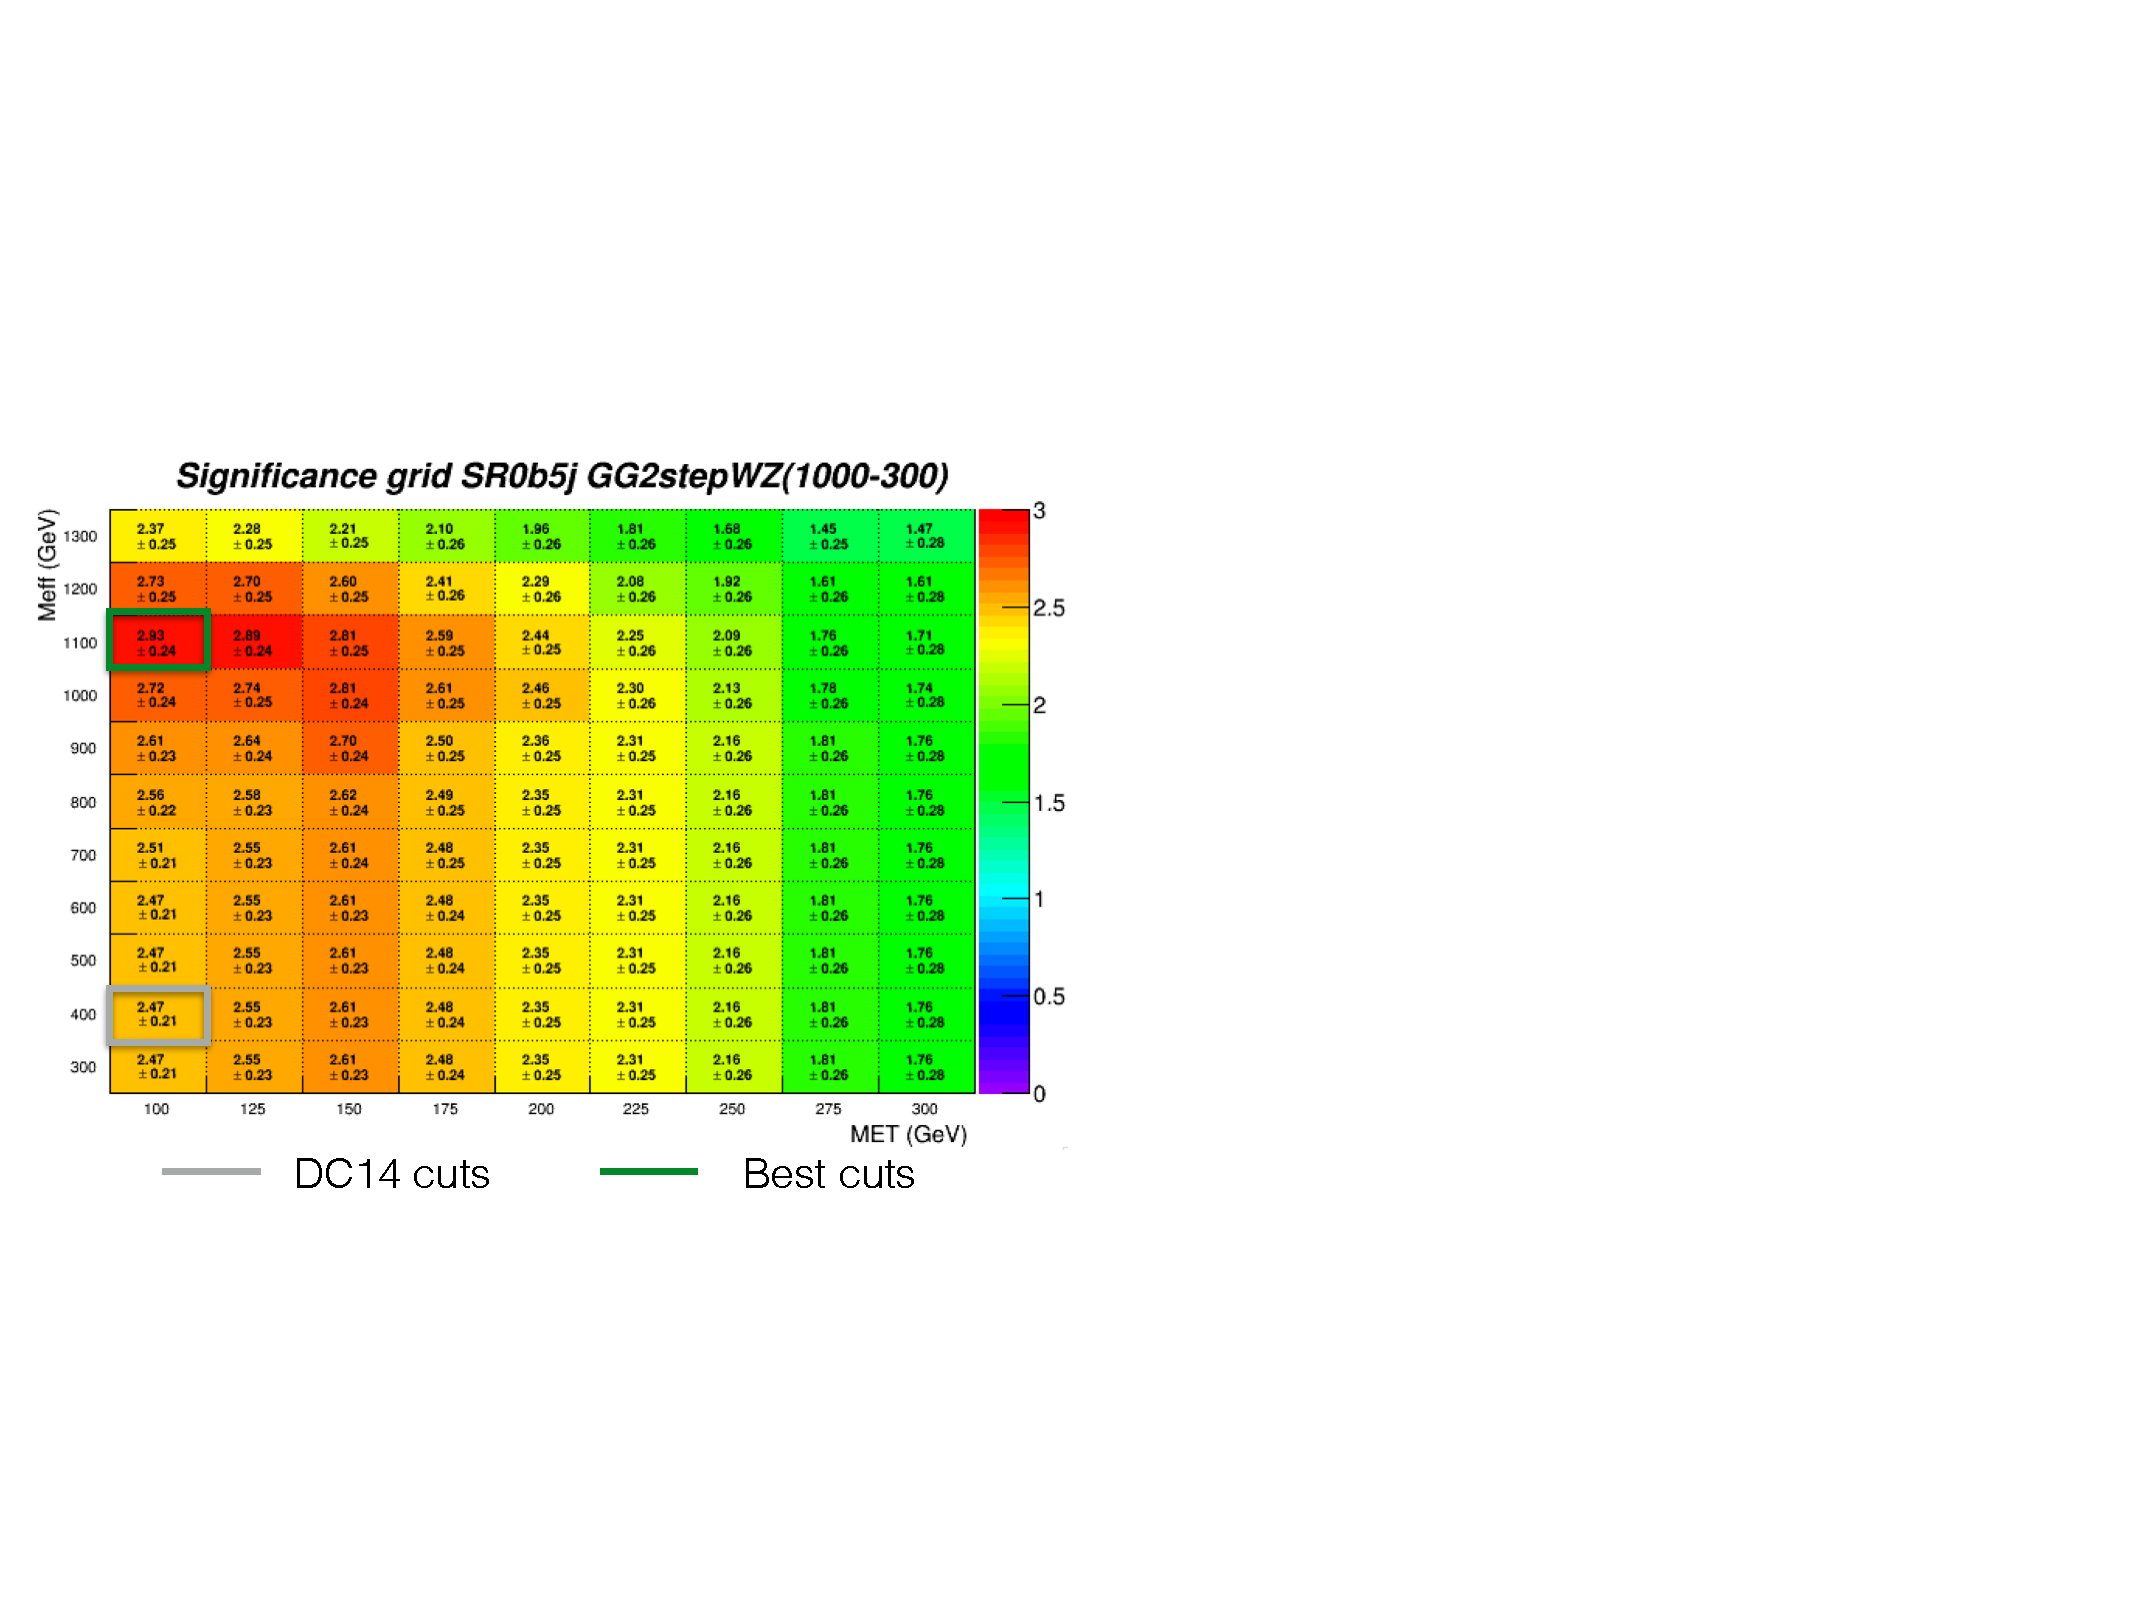
\includegraphics[width=0.49\textwidth]{OPTIMIZATION/Scan1.pdf}
  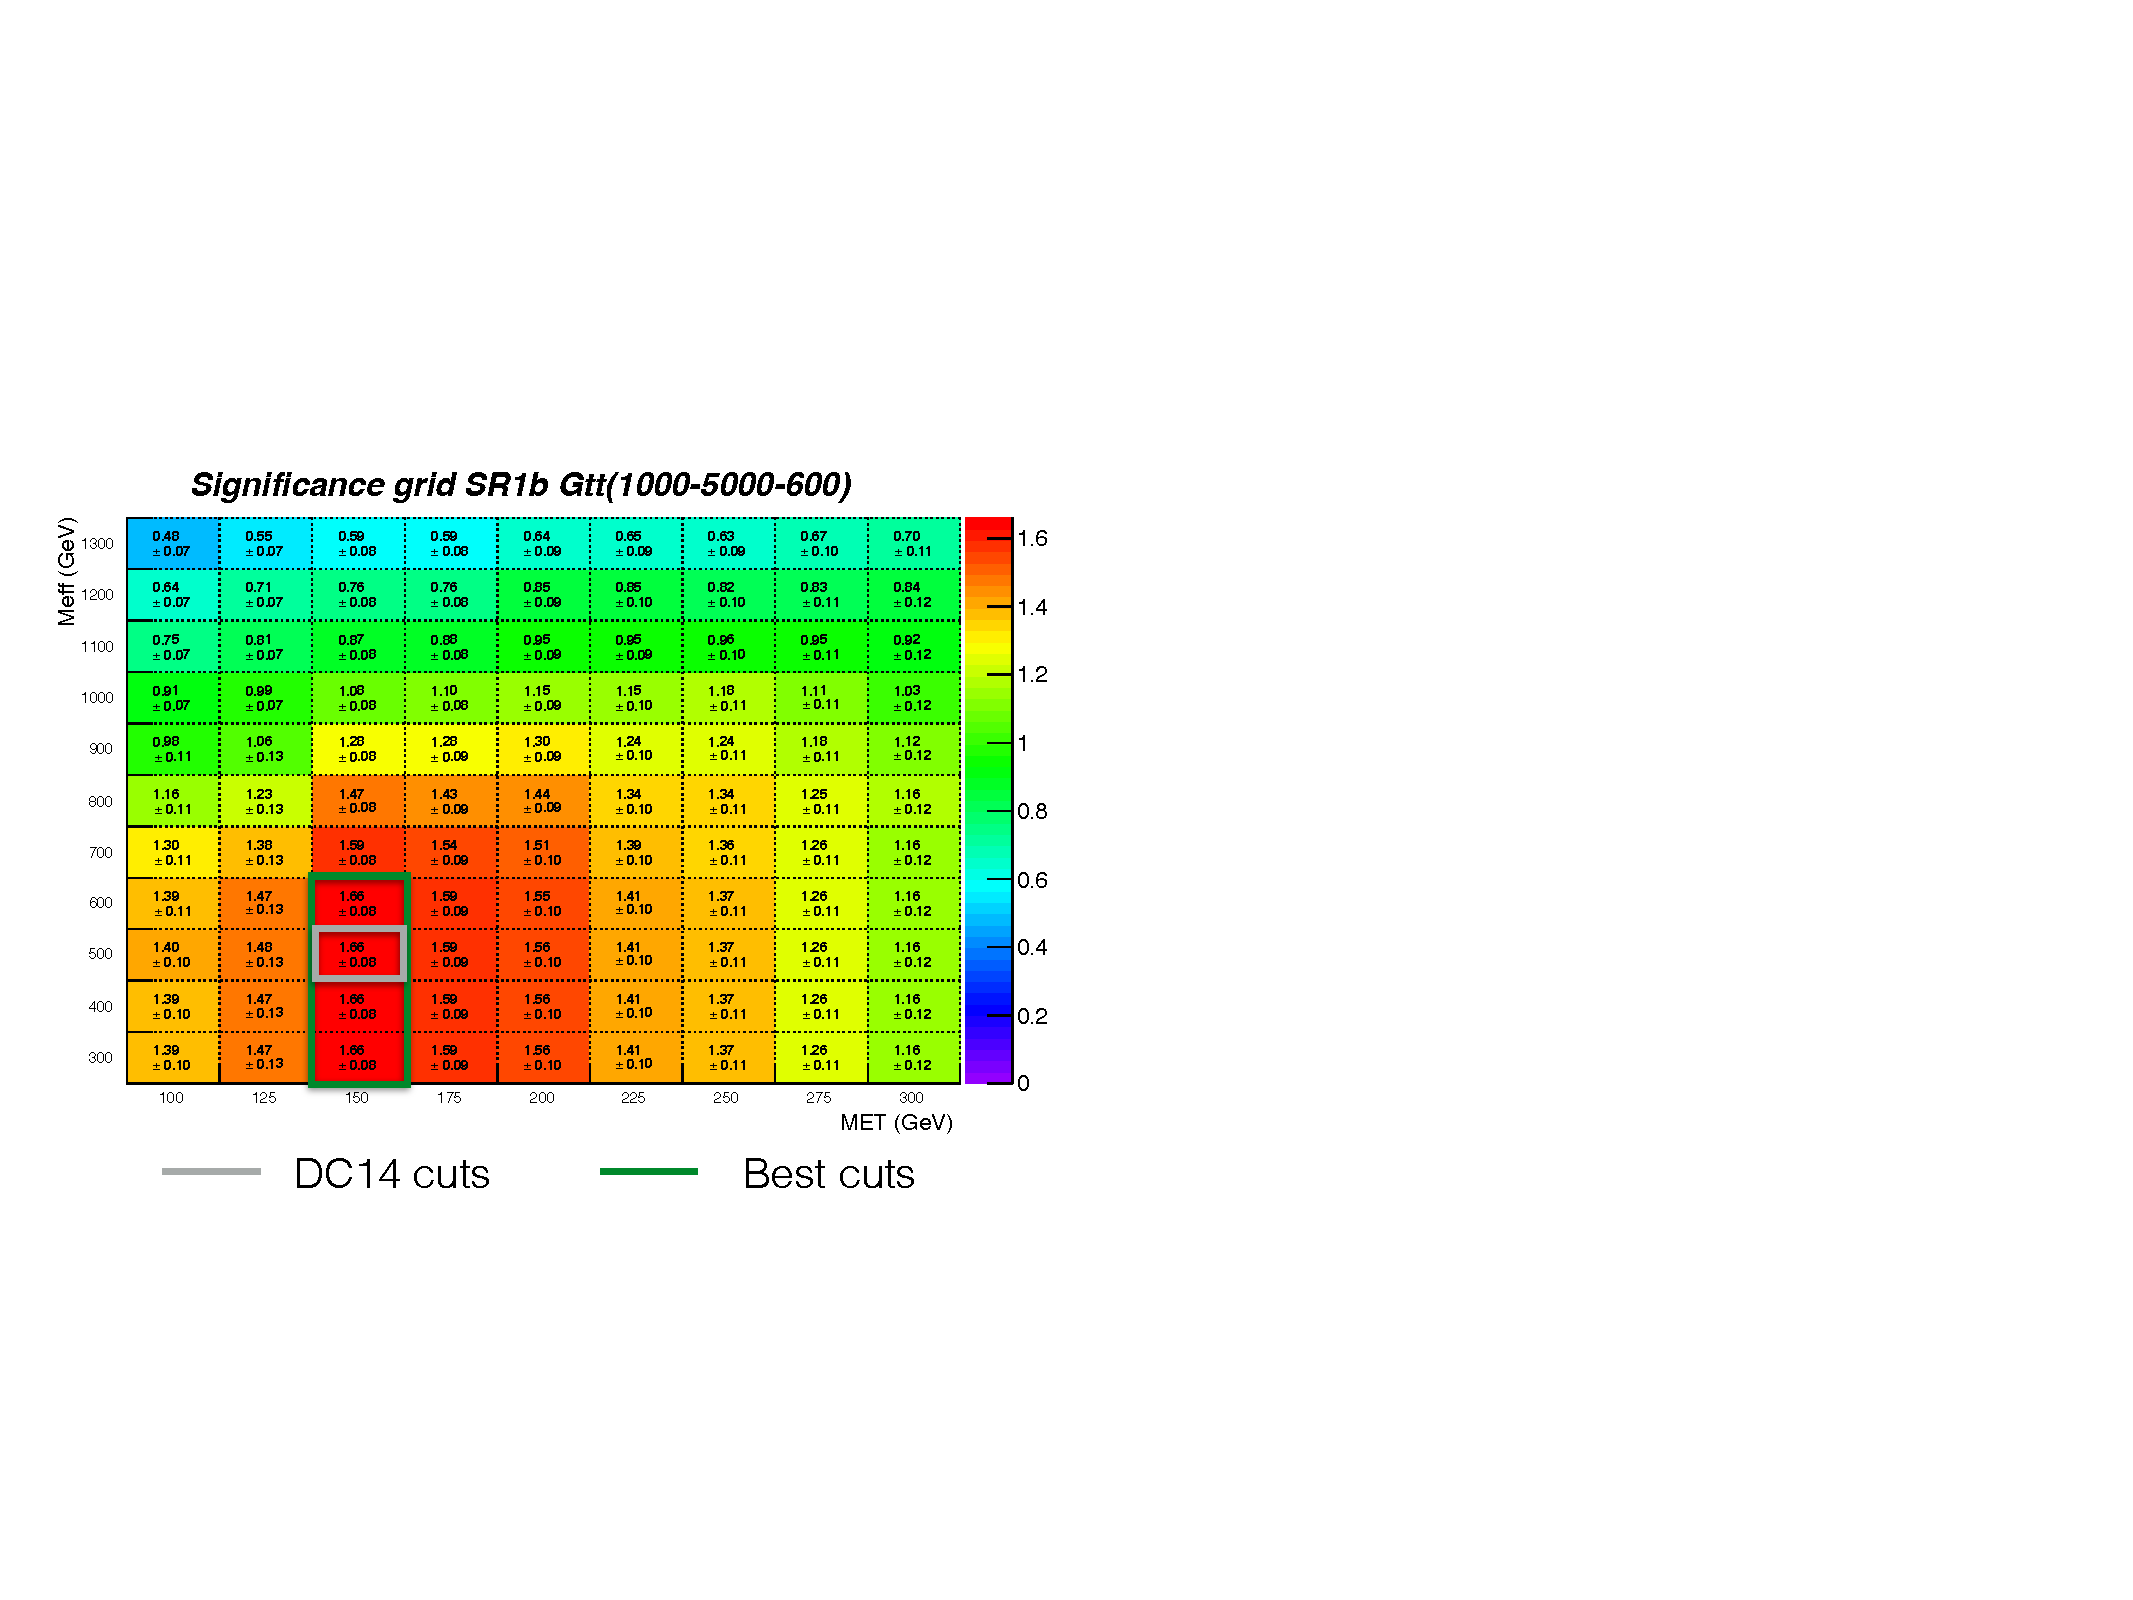
\includegraphics[width=0.49\textwidth]{OPTIMIZATION/Scan2.pdf}
  \caption{Example of (\met, \meff) scans for SR0b5j (left) and SR3b (right). The configurations with maximum significance are highlighted as well as the outcome of the DC14 optimization studies.}
\label{fig:OptimScan}


\end{figure}


%\begin{figure}[!htb]
%\centering
%  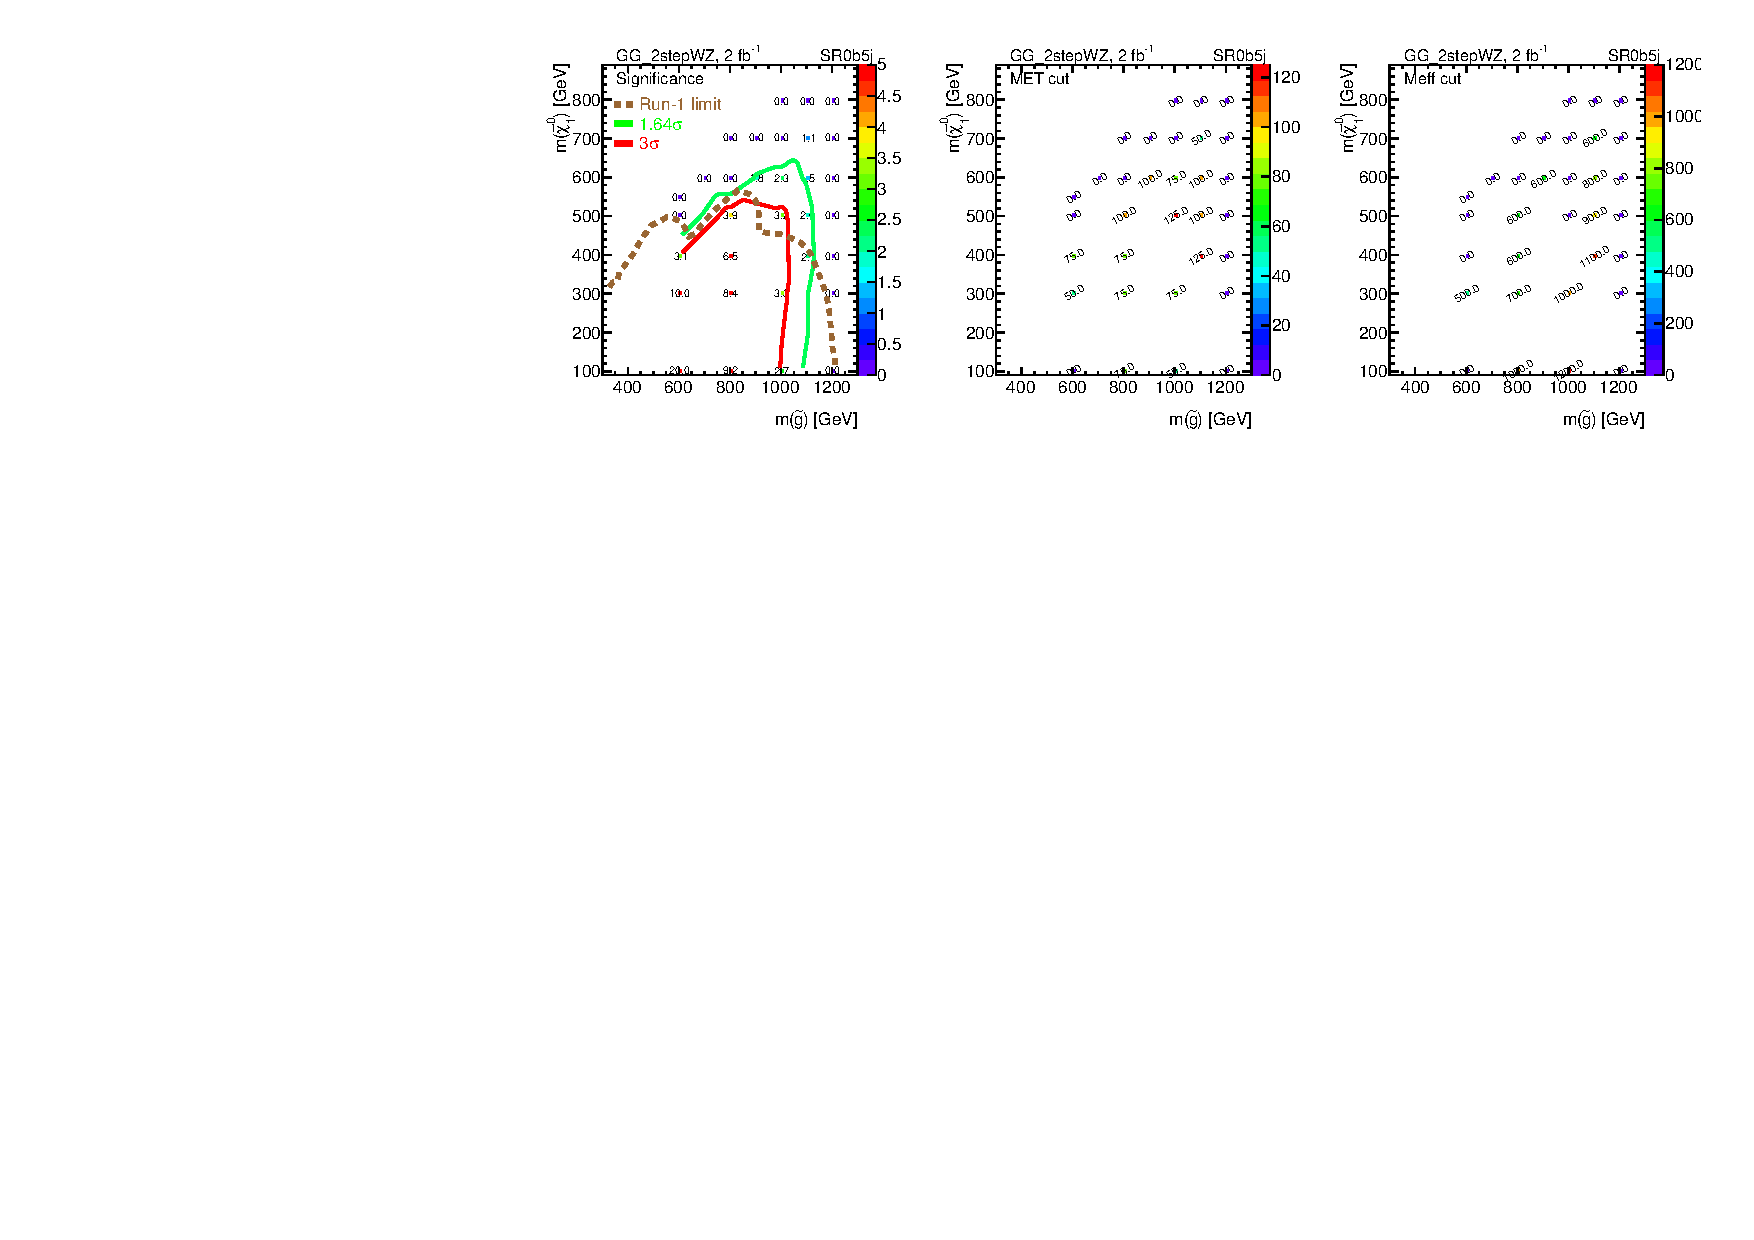
\includegraphics[width=\textwidth]{OPTIMIZATION/Optimiz_SR0b5j_2fb.pdf}
%  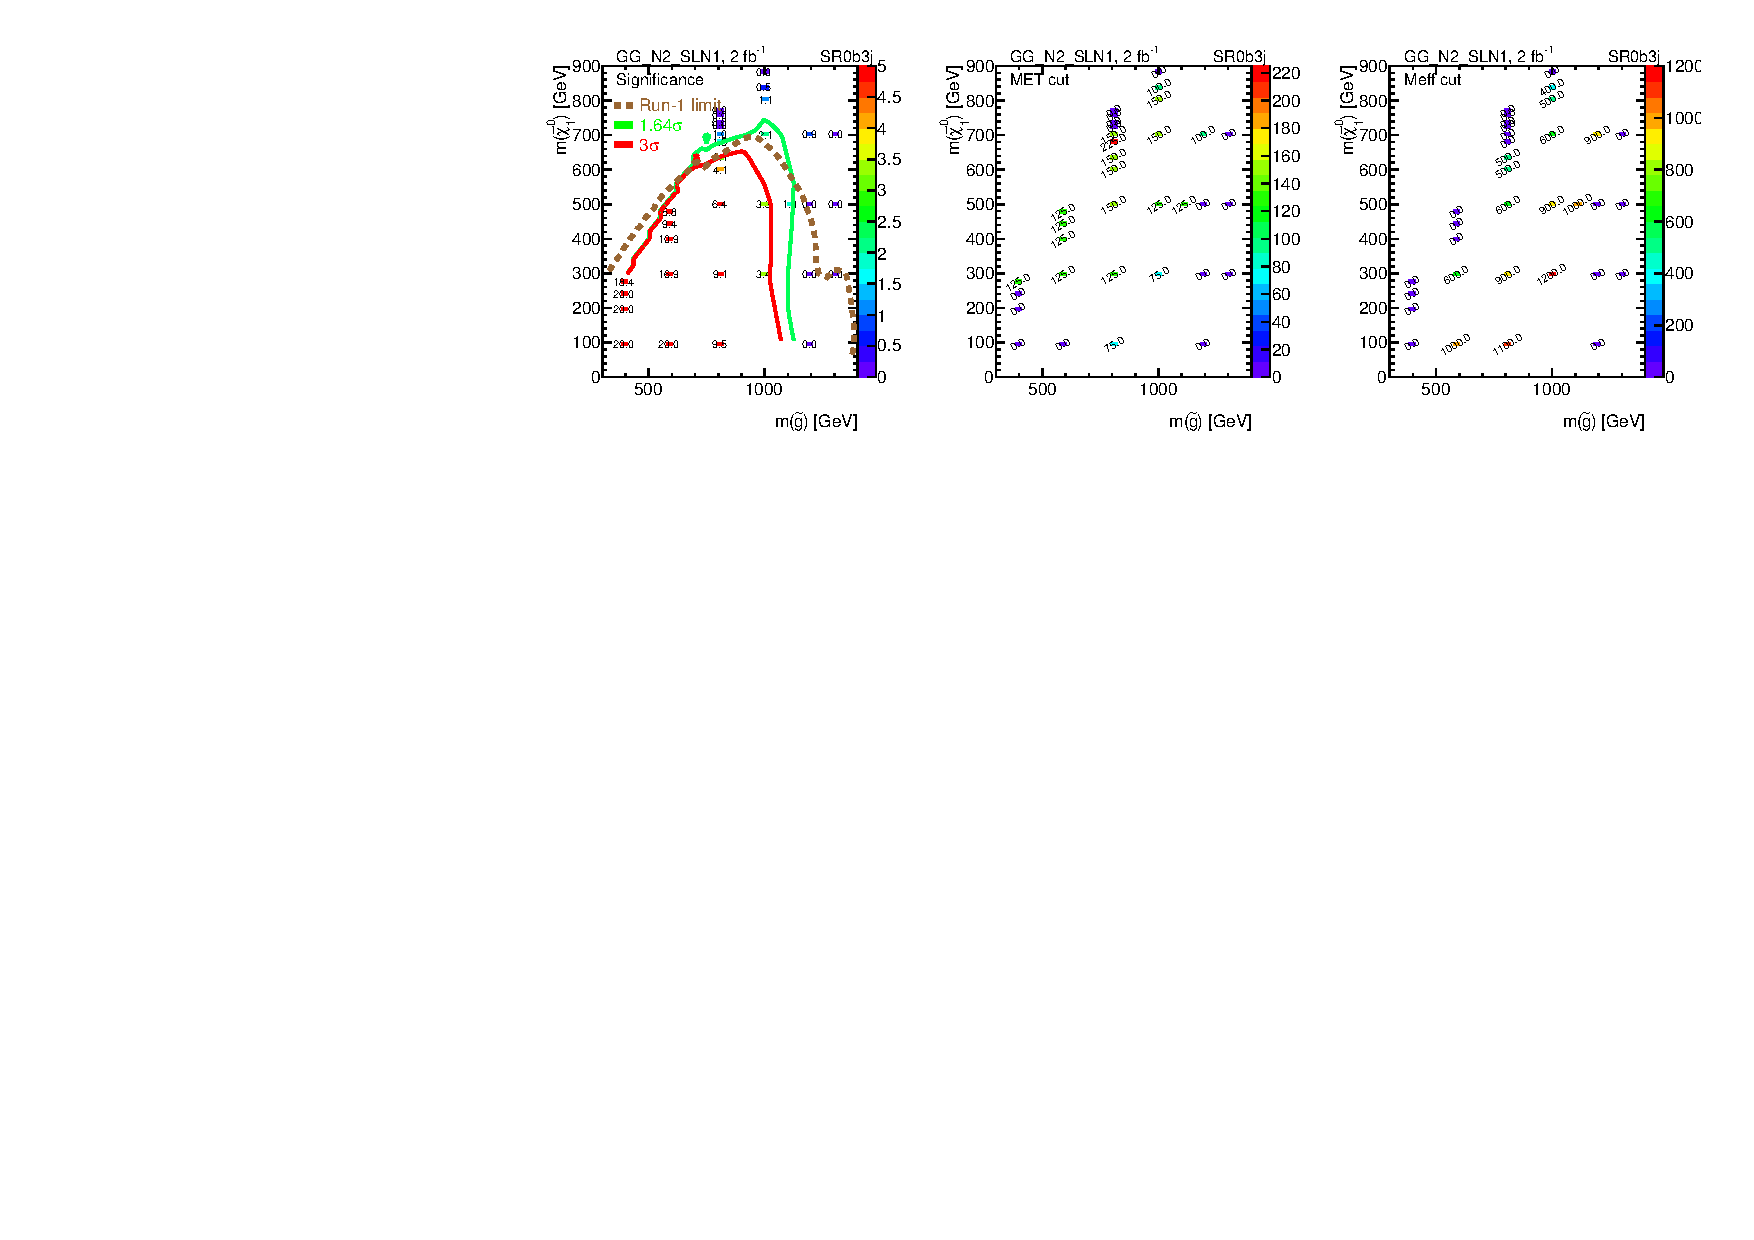
\includegraphics[width=\textwidth]{OPTIMIZATION/Optimiz_SR0b3j_2fb.pdf}
%\caption{Maximum discovery significance (left) for 2~\ifb\, as well as the $\met$ (center) and $\meff$ (right) cuts needed to maximize the significance for SR0b5j in the $\gluino\gluino$ 2-step grid (top) and SR0b3j in the $\gluino\gluino$ 1-step grid (bottom). The Run-1 limits in those models are shown with a brown line.}
%\label{fig:OptimSig2}
%\end{figure}


\subsection{Signal regions}
 
The definition of the exact SR was done as a good compromise across the signal grids shown in 
Figure~\ref{fig:OptimSig1} with a single ($\met$, $\meff$) configuration. 
Tables~\ref{tab:SRdef2}-\ref{tab:SRdef4} show the optimized signal region definitions for scenarios with 2, 3 and 4~\ifb\, respectively. 
The final SR to be used for the 2015 analysis was determined by the luminosity available at the end of the data-taking period: 
if less than 2.5~\ifb\ had been available for analysis after GRL, we would have used the SRs for the 2~\ifb\ scenario; 
if more than 3.5~\ifb\ had been available, we would have used the SRs for the 4~\ifb\ scenario. 
But with the 3.2~\ifb\ eventually collected, we used the definitions corresponding to the intermediate scenario of 3~\ifb.
Figures~\ref{fig:OptimSig2} and \ref{fig:OptimSig4} show the significance values obtained for those signal regions in the SUSY models considered, 
with the 1.64$\sigma$ discovery contours extending beyond the Run-1 exclusions, even achieving a 3$\sigma$ sensitivity in certain regions of the mass parameter space.
 
 
\begin{table}[htb!]
\caption{Signal regions definition for the 2~\ifb\ scenario (to be used for $L <2.5$~fb$^{-1}$). The two leading leptons are required to have \pt~$>$~20~\GeV.}
\hspace{0.5cm}
\label{tab:SRdef2}
\centering
\begin{tabular}{|c|c|c|c|c|c|}
\hline 
\hline
Signal region  &  $N_{\rm{lept}}$   & $N_{b\rm{-jets}}^{20}$    & $N_{\rm{jets}}^{50}$  & \met\ [GeV] & \meff\ [GeV]   \\
\hline\hline
SR3b     &   $\ge$2  &   $\ge$3  &  - & $>$100 & $>$600   \\
\hline
SR1b     &  $\ge$2  &    $\ge$1  &  $\ge$4 &  $>$125 & $>$500 \\
\hline
SR0b5j &  $\ge$2  &    $==$0 &  $\ge$5 &  $>$100 & $>$600 \\
\hline
SR0b3j &  $\ge$3  &    $==$0 &  $\ge$3 &  $>$150 & $>$500 \\
\hline\hline
\end{tabular}
\end{table}

\begin{table}[htb!]
\caption{Signal regions definition for the 3~\ifb\ scenario (to be used for $2.5 \leq L <3.5$~fb$^{-1}$), 
the one eventually used in this analysis. The two leading leptons are required to have \pt~$>$~20~\GeV.}
\hspace{0.5cm}
\label{tab:SRdef3}
\centering
\begin{tabular}{|c|c|c|c|c|c|}
\hline 
\hline
Signal region  &  $N_{\rm{lept}}$   & $N_{b\rm{-jets}}^{20}$    & $N_{\rm{jets}}^{50}$  & \met\ [GeV] & \meff\ [GeV]   \\
\hline\hline
SR3b     &   $\ge$2  &   $\ge$3  &  - & $>$125 & $>$650   \\
\hline
SR1b     &  $\ge$2  &    $\ge$1  &  $\ge$4 &  $>$150 & $>$550 \\
\hline
SR0b5j &  $\ge$2  &    $==$0 &  $\ge$5 &  $>$125 & $>$650 \\
\hline
SR0b3j &  $\ge$3  &    $==$0 &  $\ge$3 &  $>$200 & $>$550 \\
\hline\hline
\end{tabular}
\end{table}

\begin{table}[htb!]
\caption{Signal regions definition for the 4~\ifb\ scenario (to be used for $L \geq 3.5$~fb$^{-1}$). The two leading leptons are required to have \pt~$>$~20~\GeV.}
\hspace{0.5cm}
\label{tab:SRdef4}
\centering
\begin{tabular}{|c|c|c|c|c|c|}
\hline 
\hline
Signal region  &  $N_{\rm{lept}}$   & $N_{b\rm{-jets}}^{20}$    & $N_{\rm{jets}}^{50}$  & \met\ [GeV] & \meff\ [GeV]   \\
\hline\hline
SR3b     &   $\ge$2  &   $\ge$3  &  - & $>$125 & $>$700   \\
\hline
SR1b     &  $\ge$2  &    $\ge$1  &  $\ge$4 &  $>$150 & $>$600 \\
\hline
SR0b5j &  $\ge$2  &    $==$0 &  $\ge$5 &  $>$125 & $>$700 \\
\hline
SR0b3j &  $\ge$3  &    $==$0 &  $\ge$3 &  $>$200 & $>$600 \\
\hline\hline
\end{tabular}
\end{table}

\begin{figure}[!htb]
\centering
  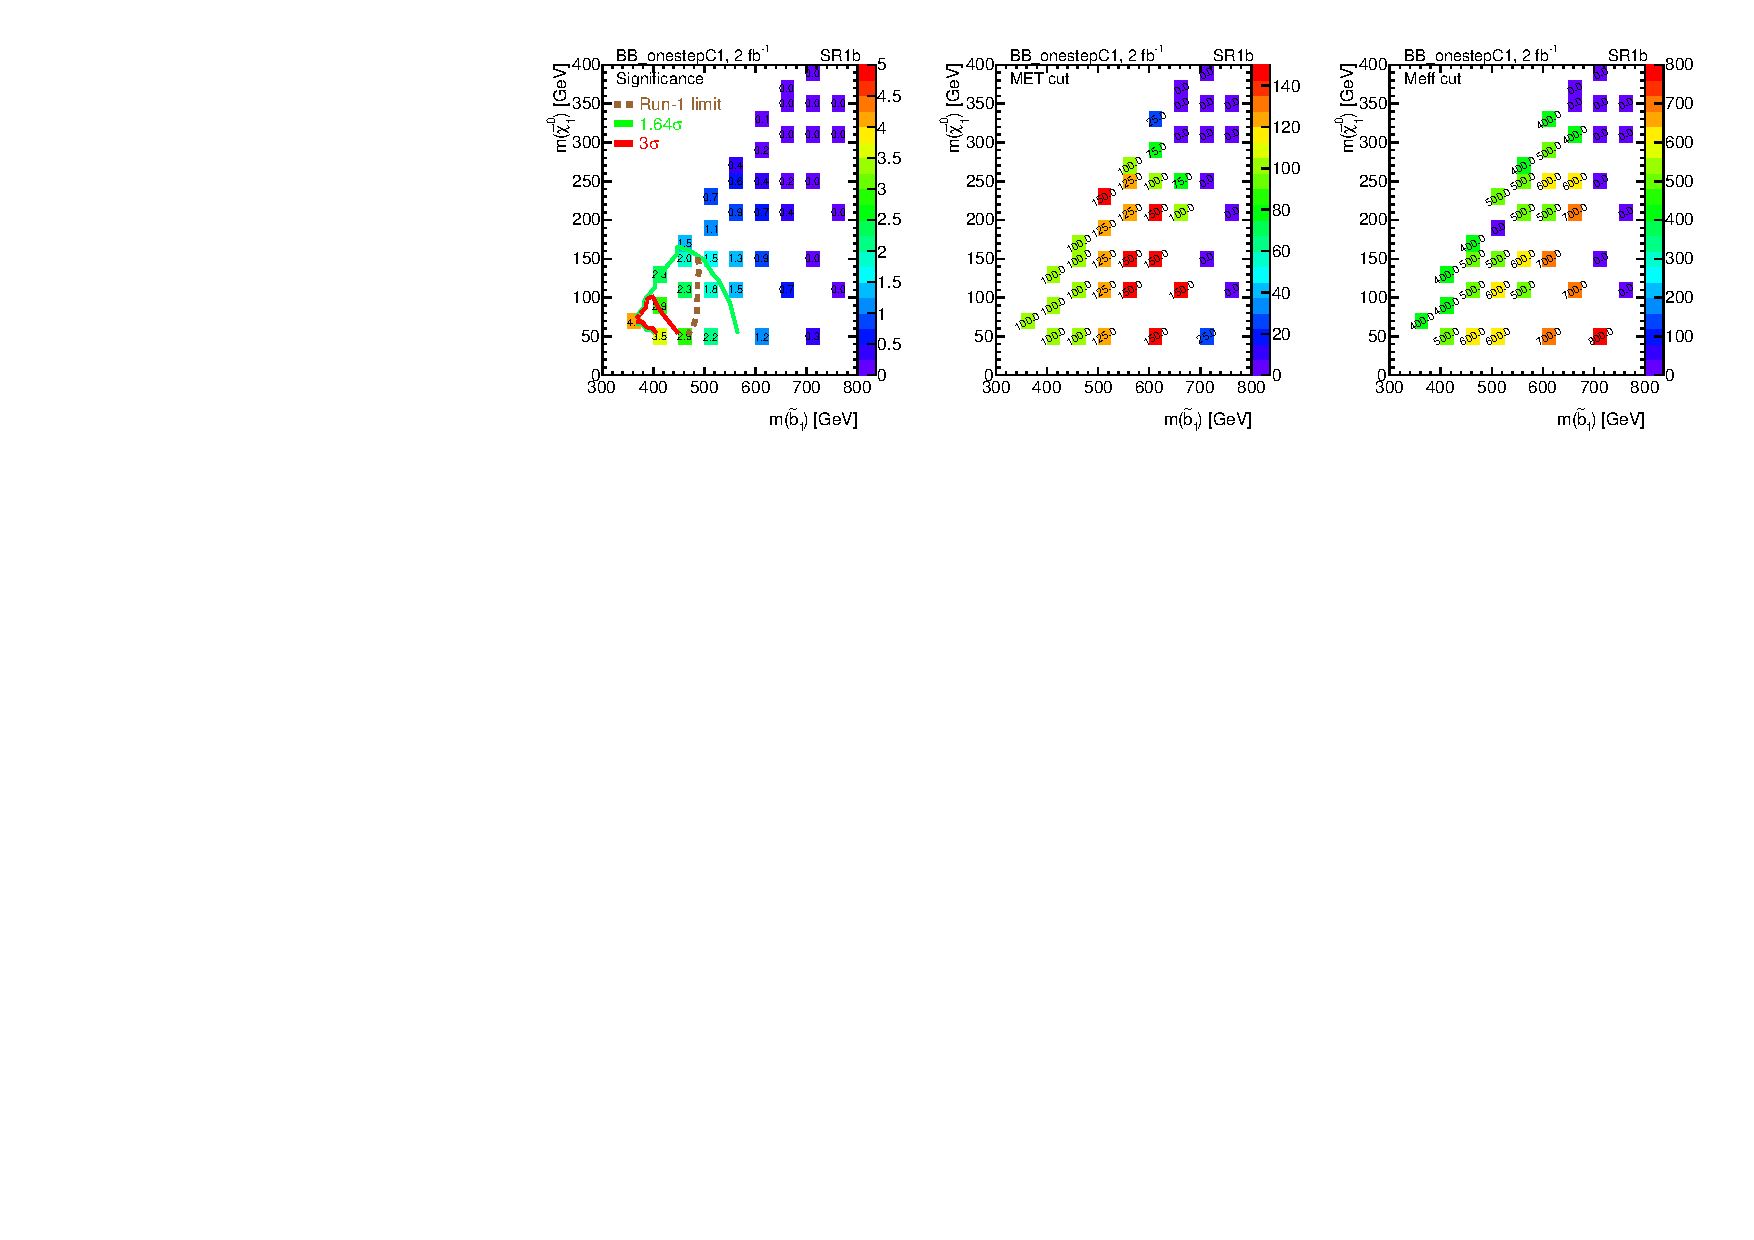
\includegraphics[width=0.9\textwidth]{OPTIMIZATION/Optimiz_SR1b_2fb.pdf}
  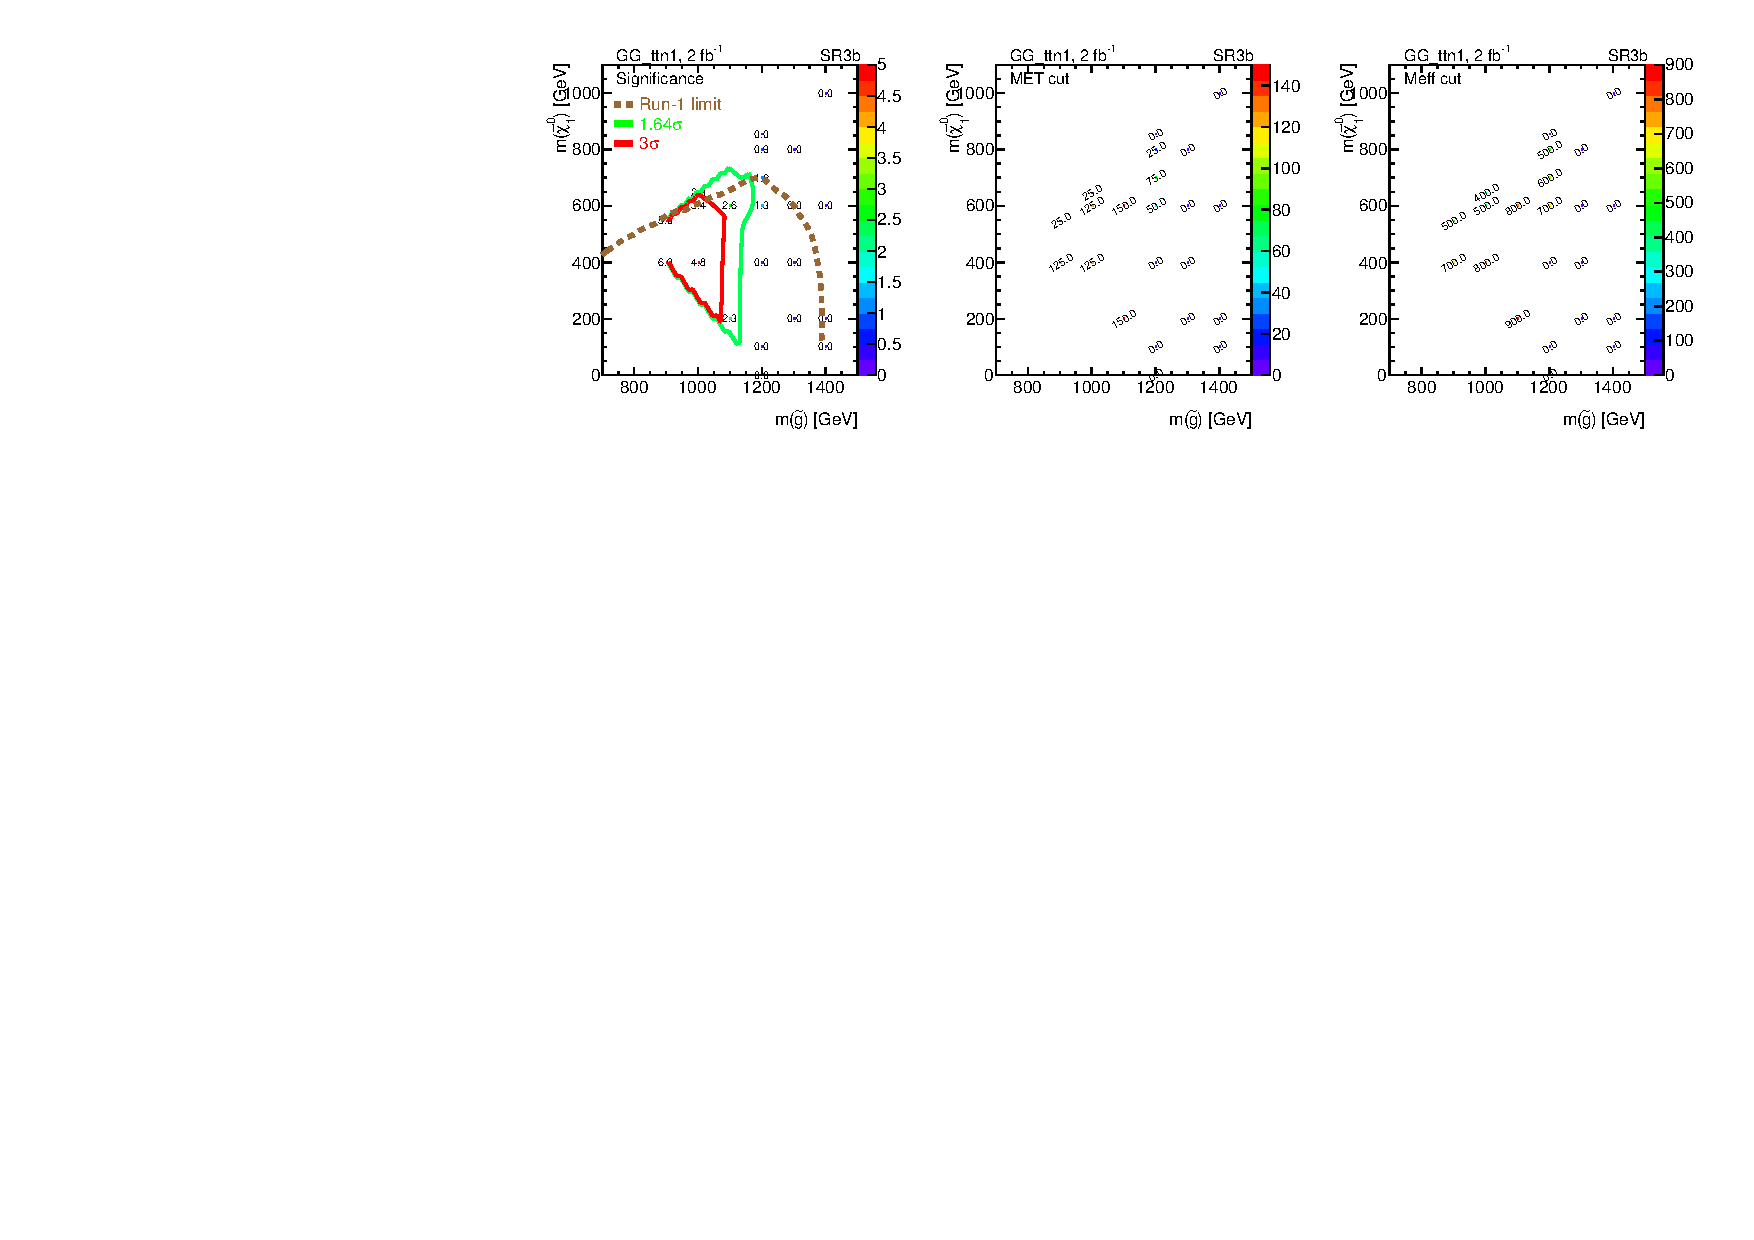
\includegraphics[width=0.9\textwidth]{OPTIMIZATION/Optimiz_SR3b_2fb.pdf}
  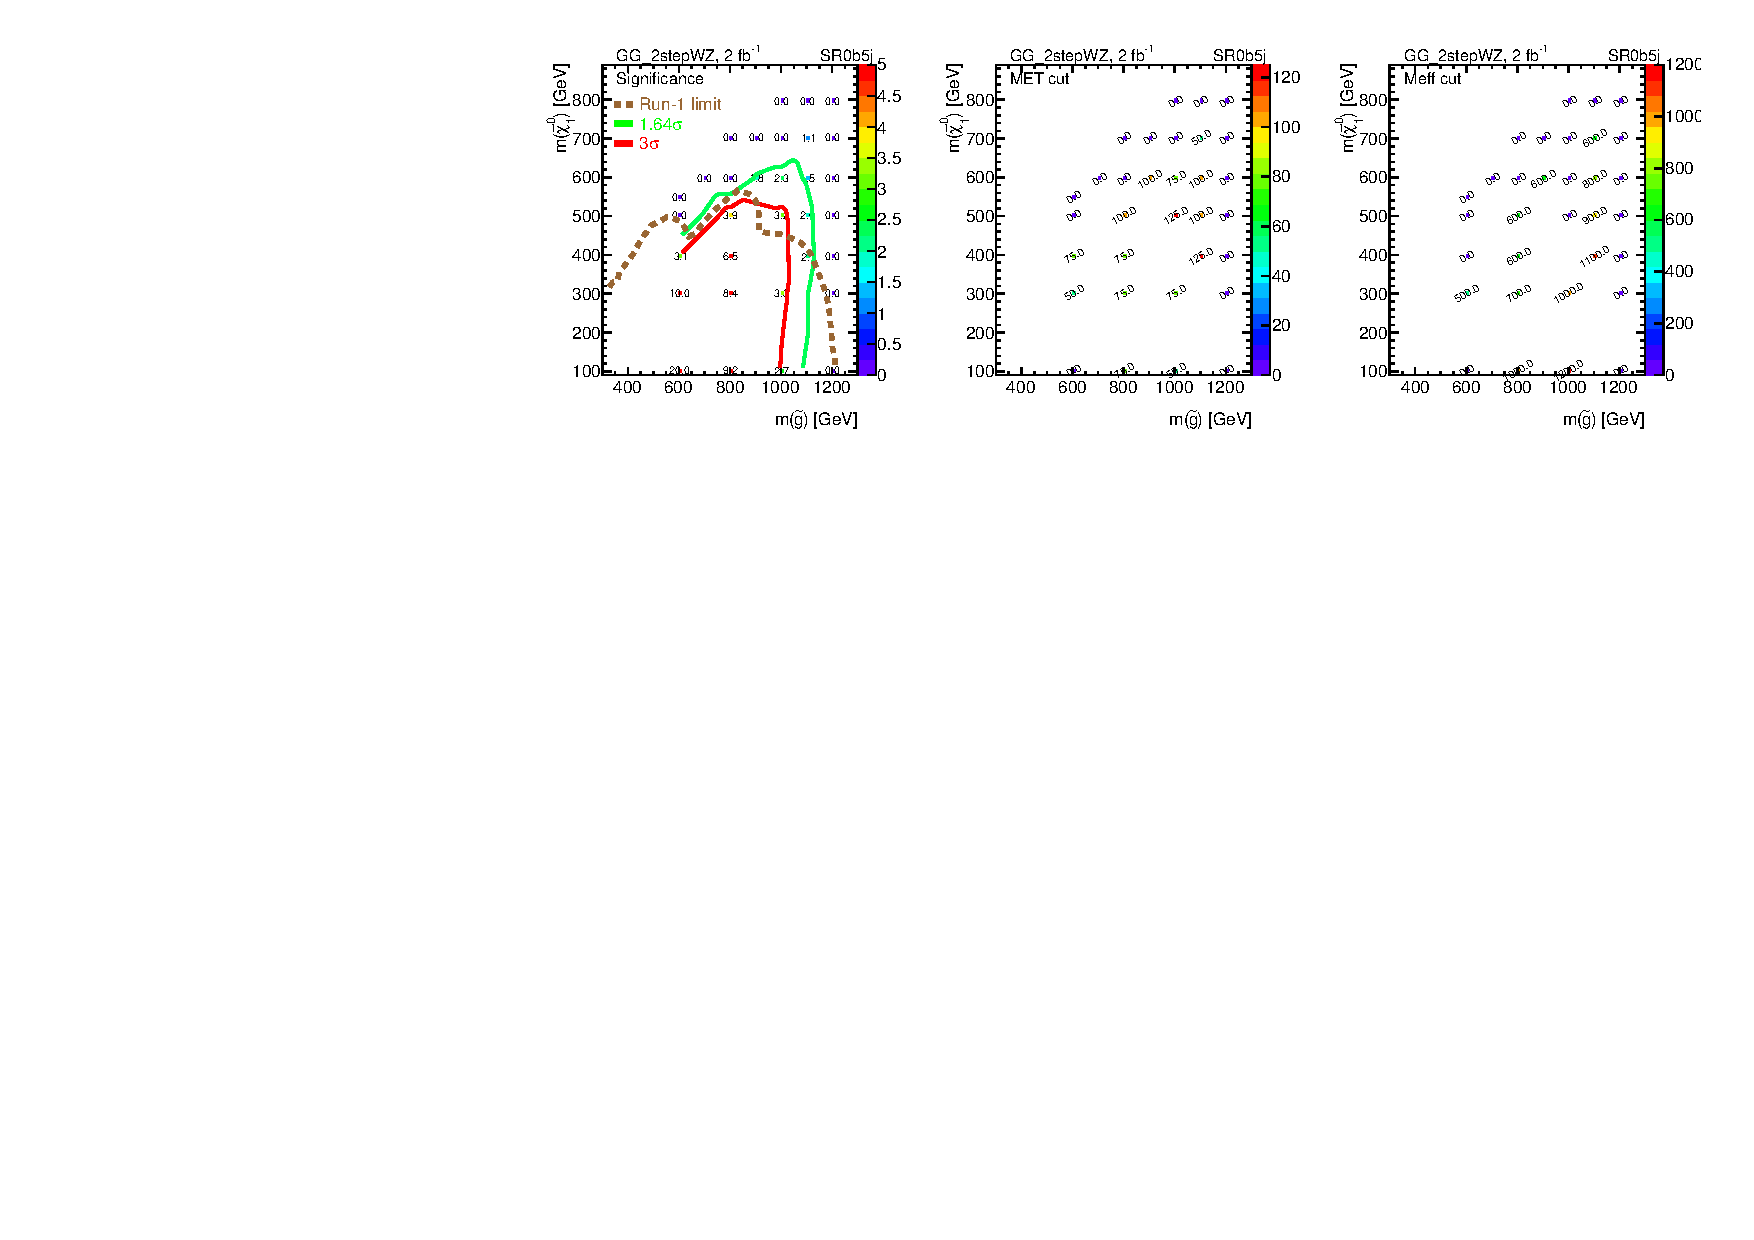
\includegraphics[width=0.9\textwidth]{OPTIMIZATION/Optimiz_SR0b5j_2fb.pdf}
  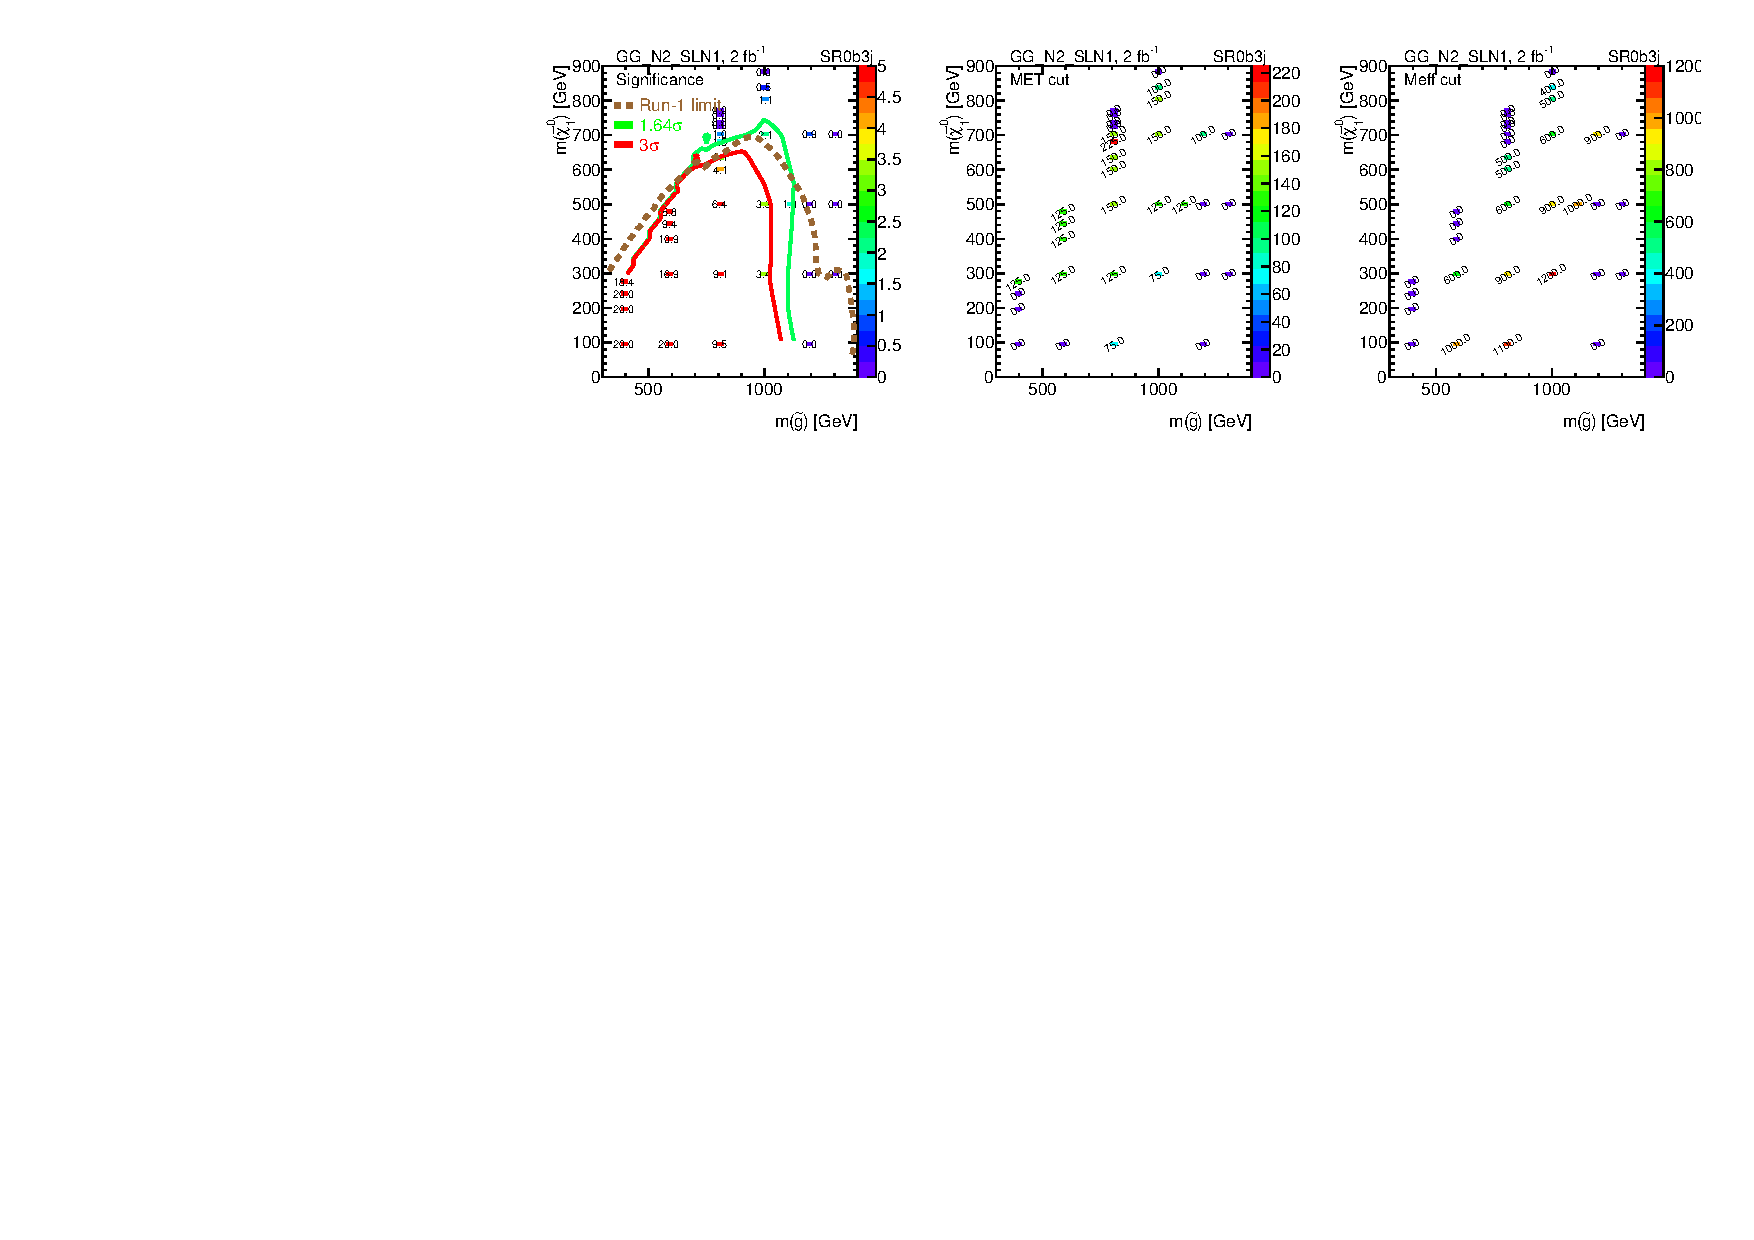
\includegraphics[width=0.9\textwidth]{OPTIMIZATION/Optimiz_SR0b3j_2fb.pdf}
  \caption{Maximum discovery significance (left) for 2~\ifb, as well as the $\met$ (center) and $\meff$ (right) cuts needed to maximize the significance for: (from top to bottom) SR1b in the $\sbot\sbot^*\to t\bar t\tilde\chi_1^+\tilde\chi_1^-$ grid, SR3b in the $\gluino\gluino\to t\bar tt\bar t\ninoone\ninoone$ grid, SR0b5j in the $\gluino\gluino$ with $\gluino\to q\bar{q}'WZ\ninoone$ grid and SR0b3j in the $\gluino\gluino$ with $\gluino\to q\bar{q}(\ell\ell/\ell\nu)\ninoone$ grid. The Run-1 limits in those models are shown with a brown line, and the 1.64$\sigma$ and 3$\sigma$ discovery contours from the proposed signal regions are shown in green and red, respectively.}
\label{fig:OptimSig1}
\end{figure}



\begin{figure}[!htb]
\centering
  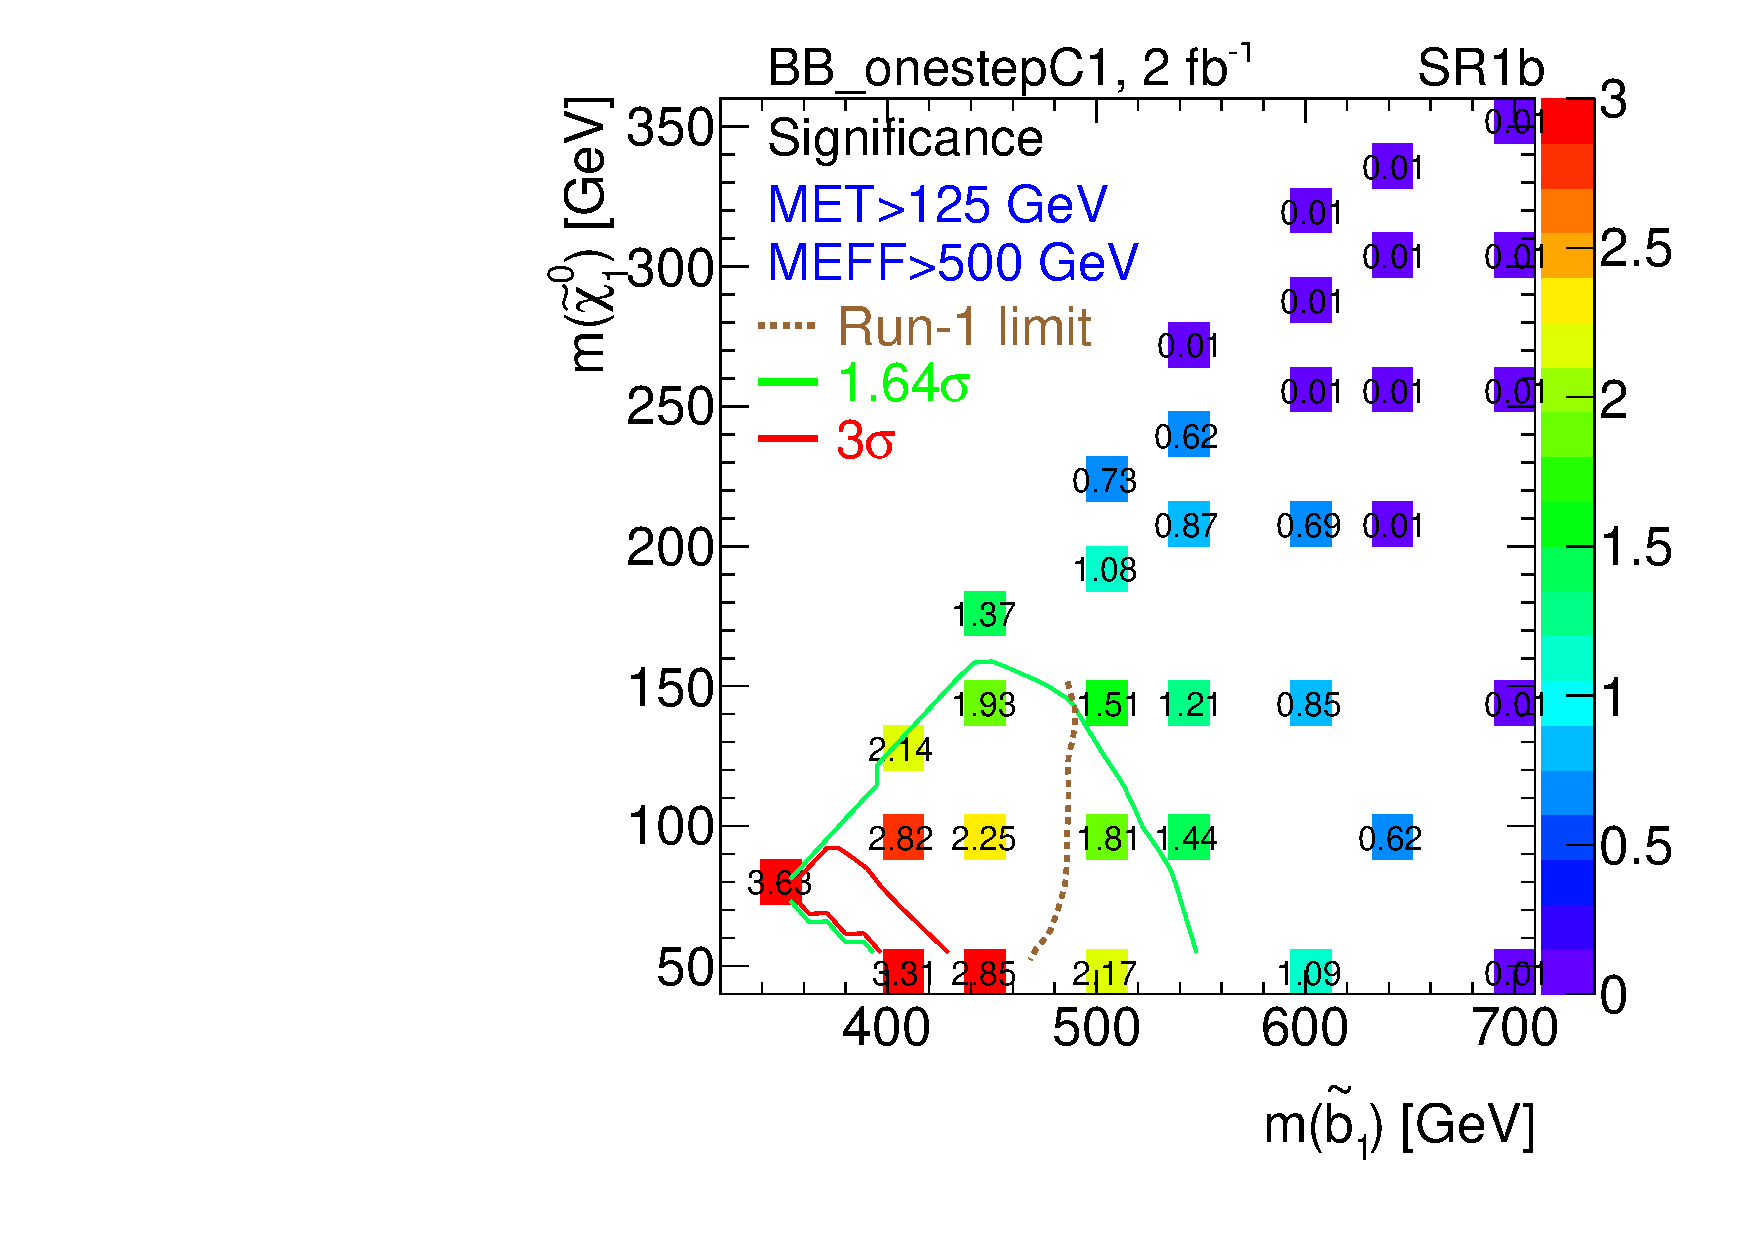
\includegraphics[width=0.4\textwidth]{OPTIMIZATION/Optimiz_SR1b_2fb_125_500.pdf}
  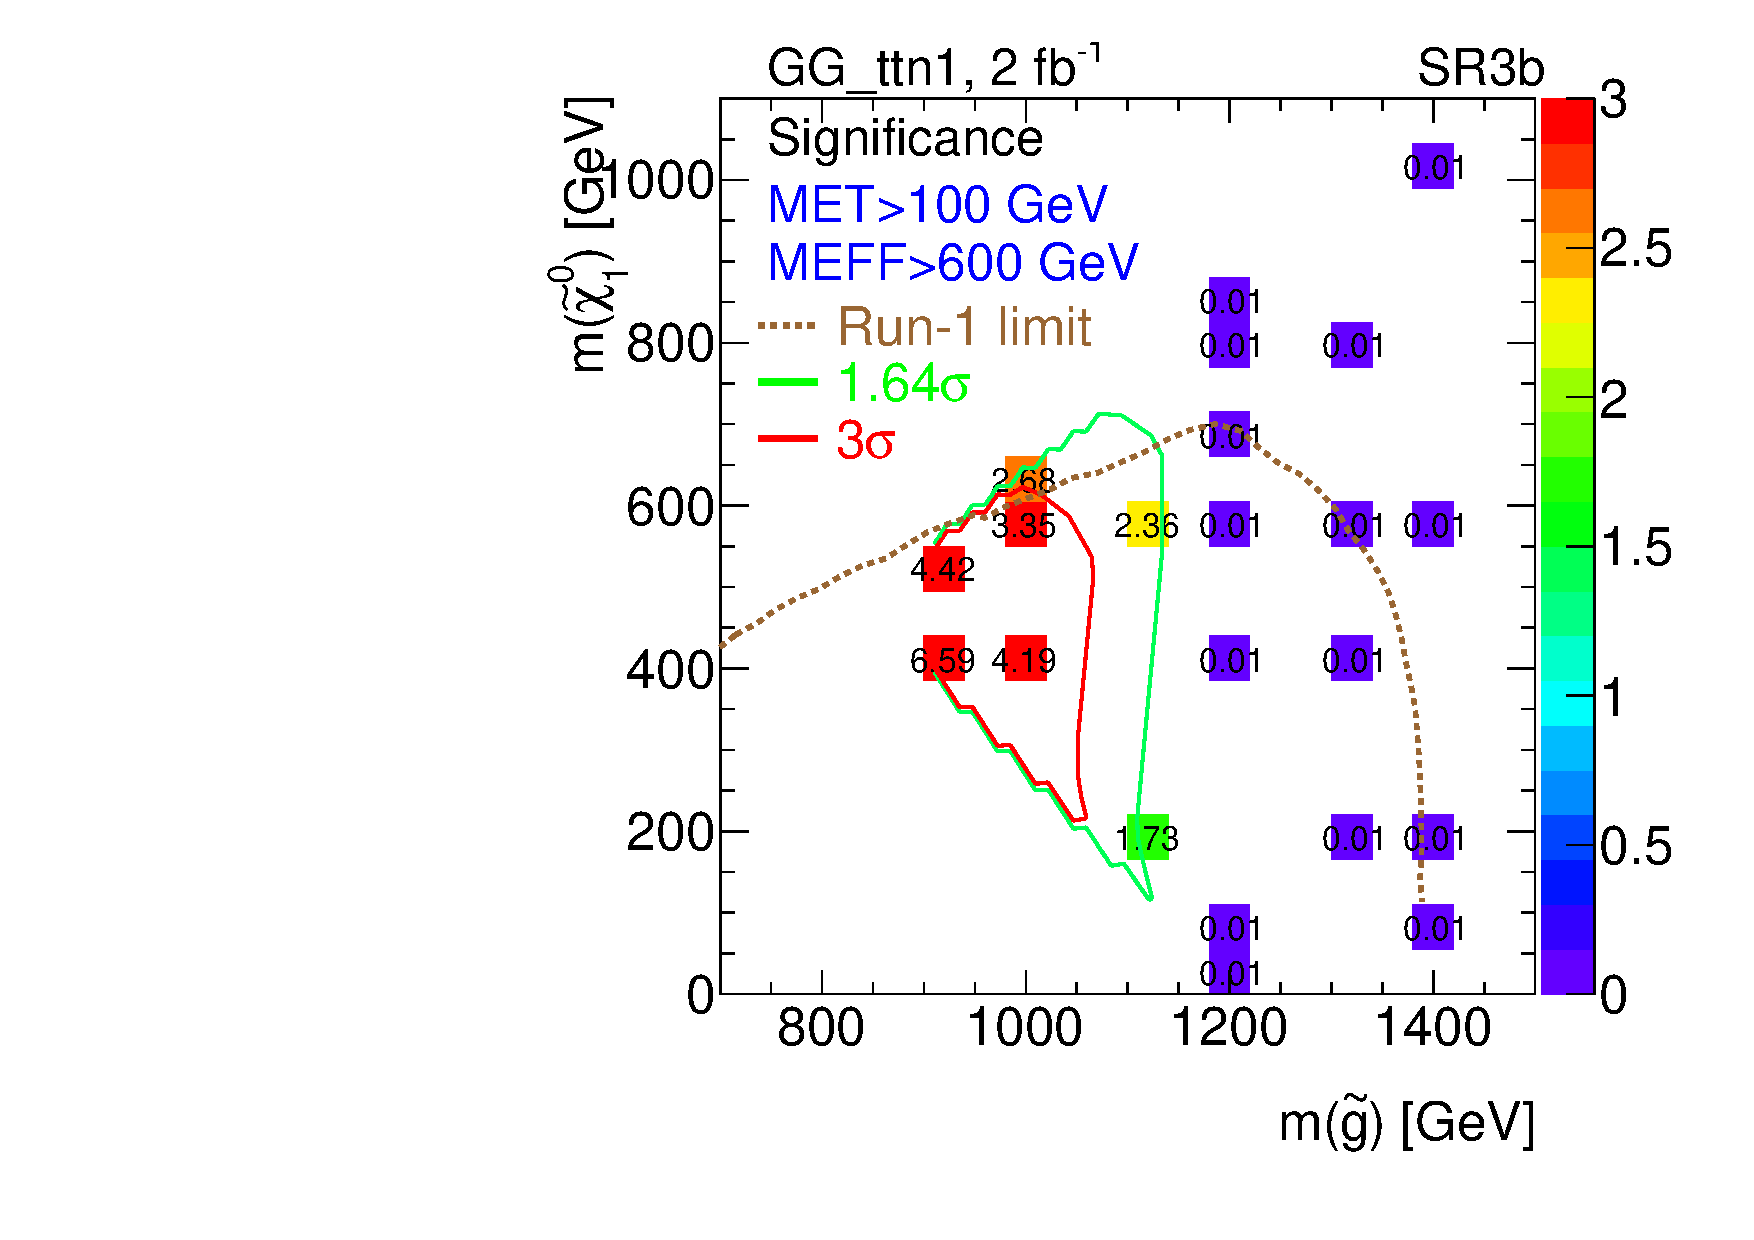
\includegraphics[width=0.4\textwidth]{OPTIMIZATION/Optimiz_SR3b_2fb_100_600.pdf}\\
  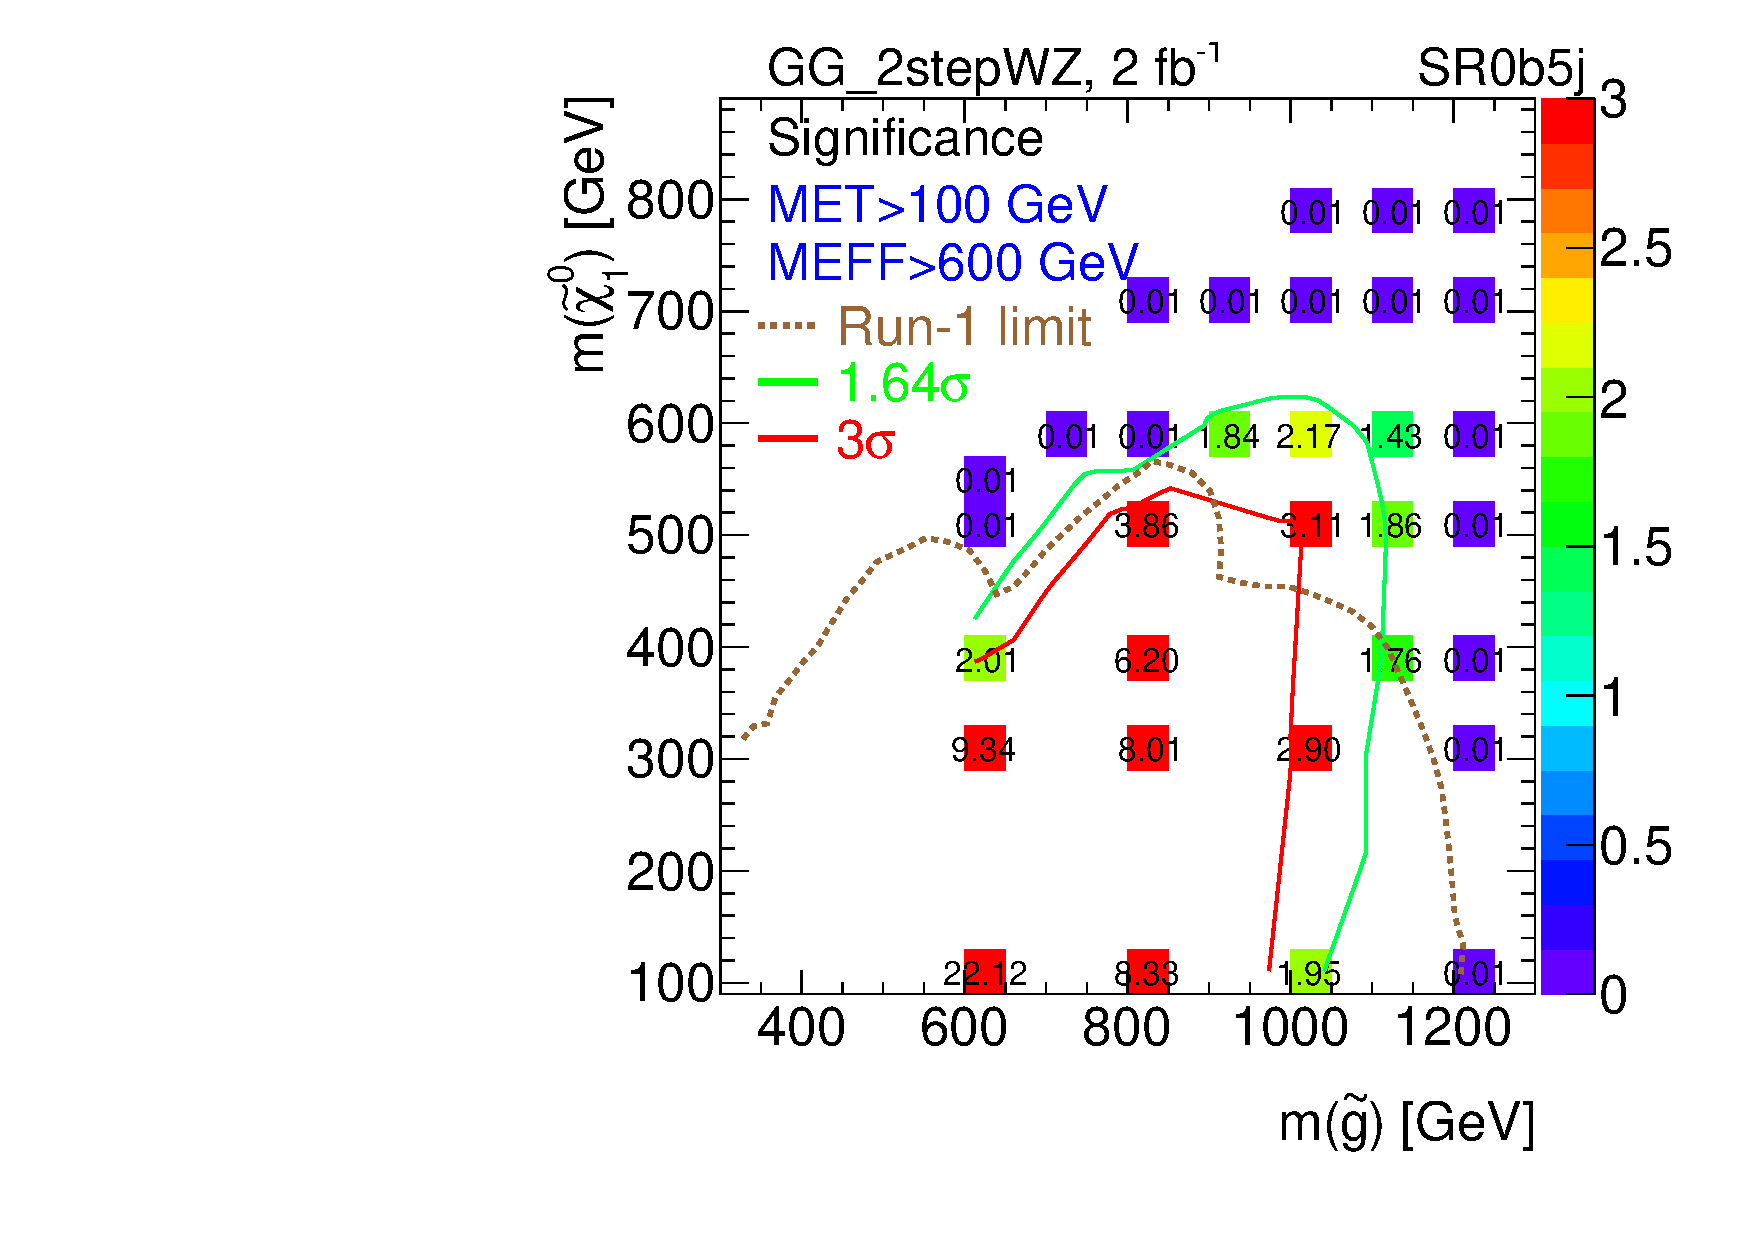
\includegraphics[width=0.4\textwidth]{OPTIMIZATION/Optimiz_SR0b5j_2fb_100_600.pdf}
  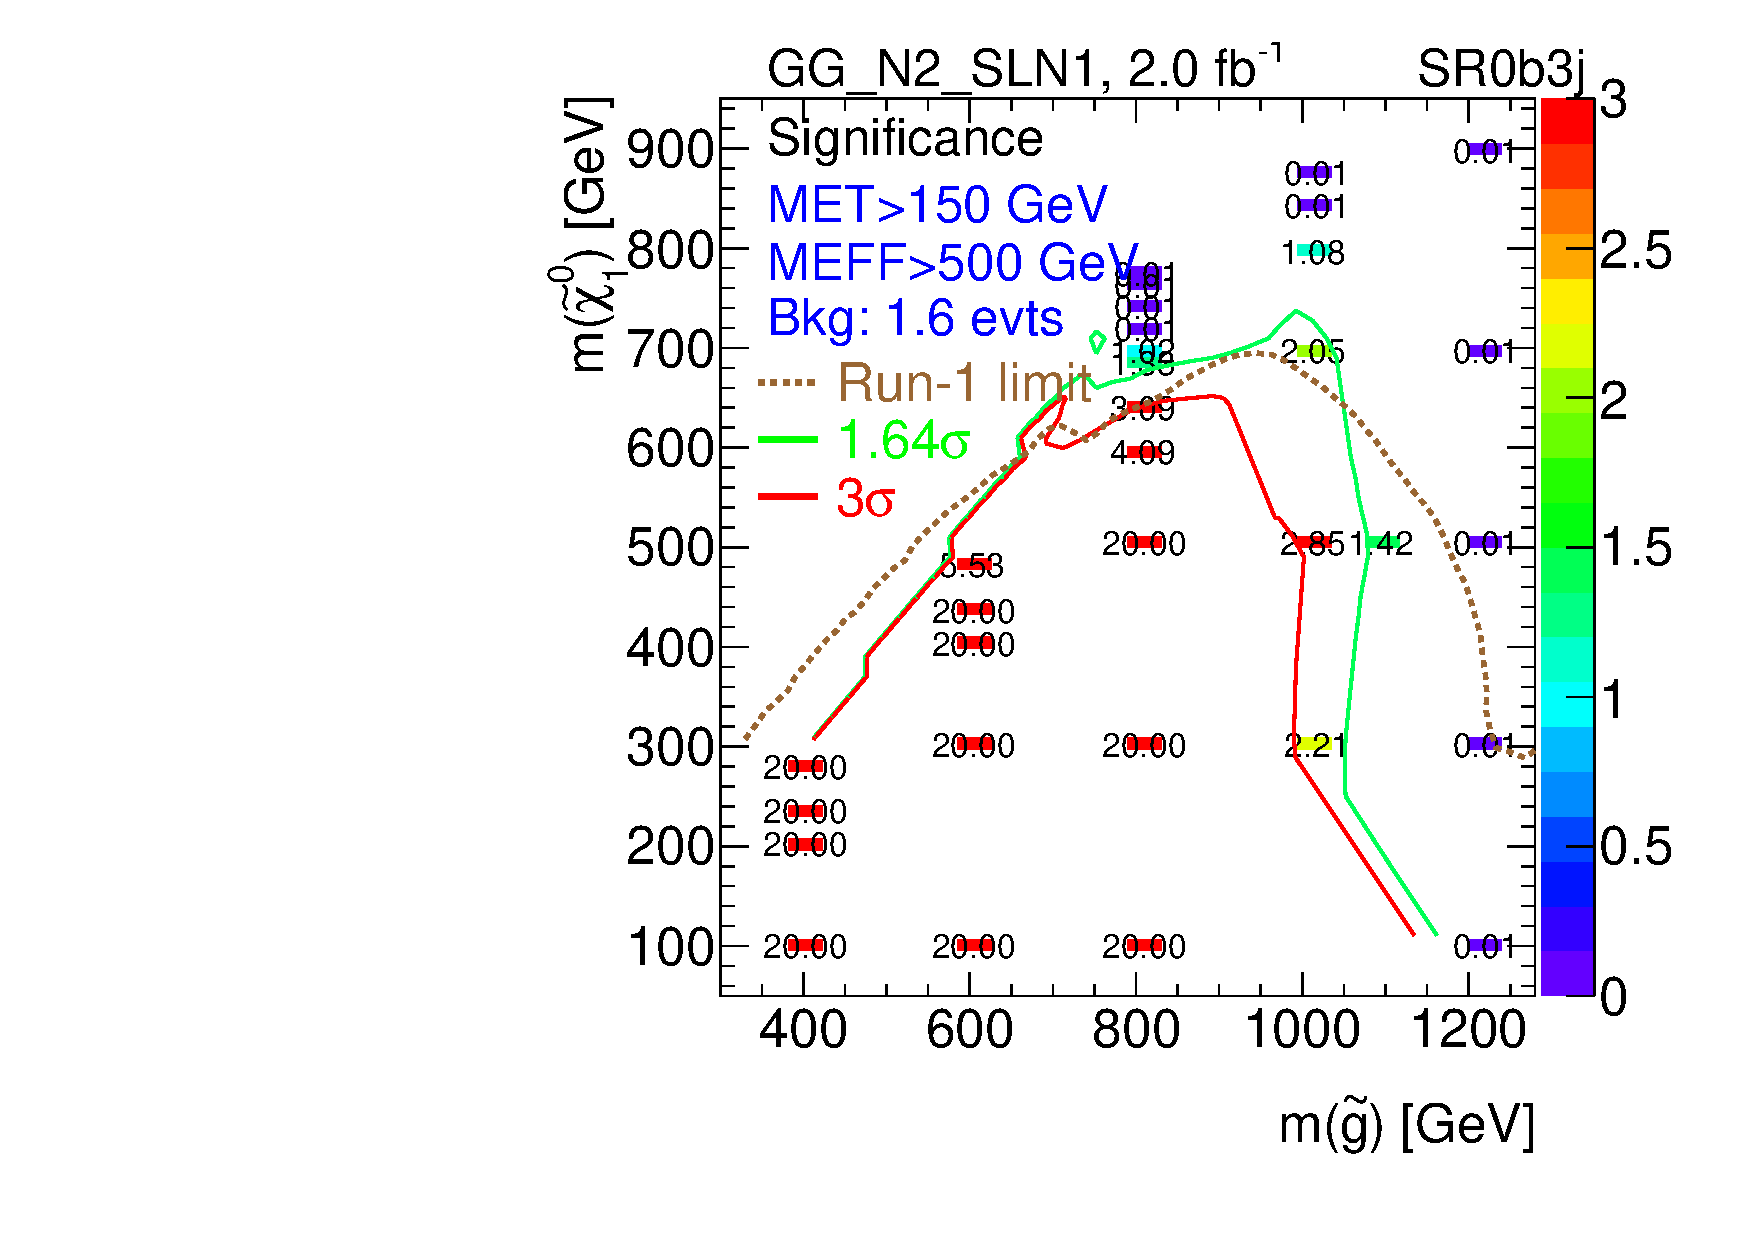
\includegraphics[width=0.4\textwidth]{OPTIMIZATION/Optimiz_SR0b3j_2fb_150_500.pdf}
  \caption{Discovery significance for the SRs defined in Table~\ref{tab:SRdef2} (2~\ifb) for SR1b in the $\sbot\sbot^*\to t\bar t\tilde\chi_1^+\tilde\chi_1^-$ grid (top left), SR3b in the $\gluino\gluino\to t\bar tt\bar t\ninoone\ninoone$ grid (top right), SR0b5j in the $\gluino\gluino$ with $\gluino\to q\bar{q}'WZ\ninoone$ grid (bottom left) and SR0b3j in the $\gluino\gluino$ with $\gluino\to q\bar{q}(\ell\ell/\ell\nu)\ninoone$ grid (bottom right). The Run-1 limits in those models are shown with a brown line, and the 1.64$\sigma$ and 3$\sigma$ discovery contours from the proposed signal regions are shown in green and red, respectively.}
\label{fig:OptimSig2}
\end{figure}


\begin{figure}[!htb]
\centering
  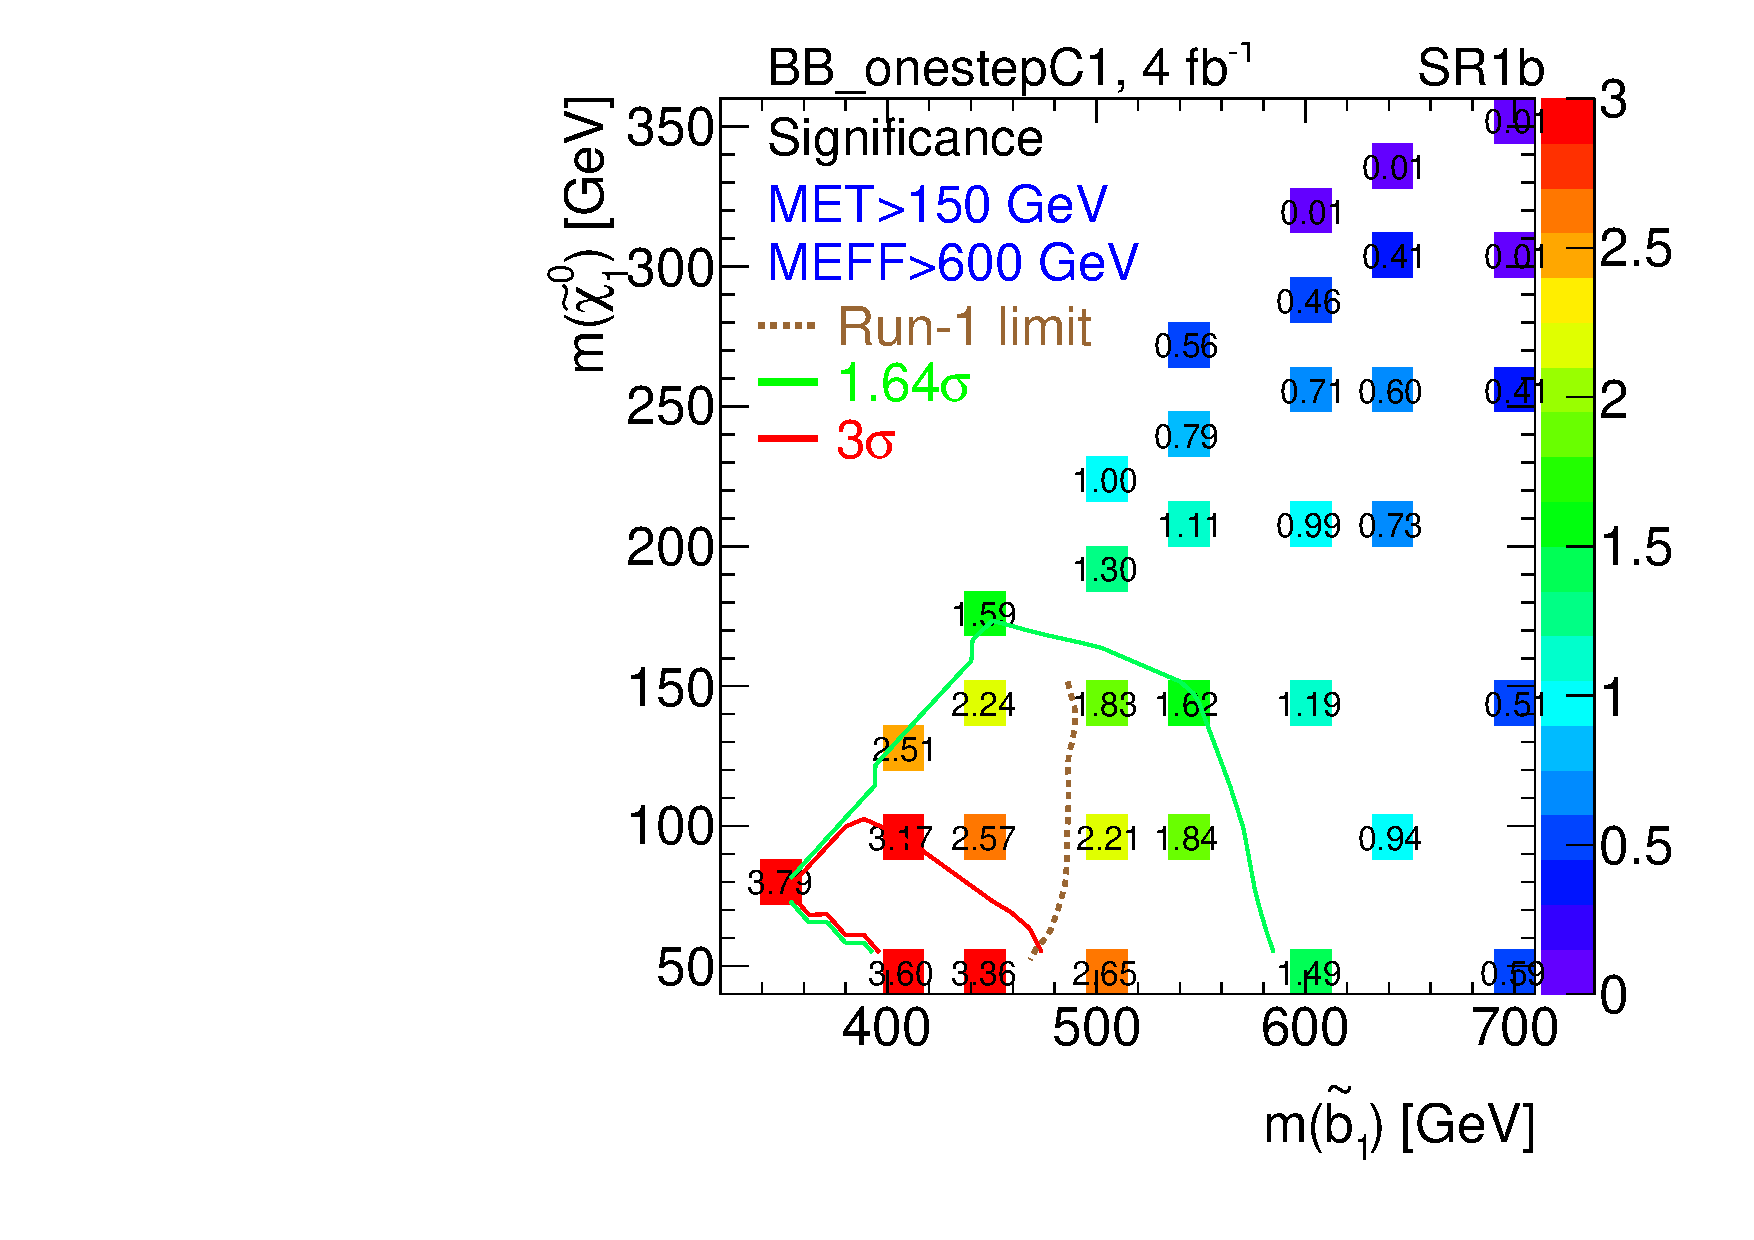
\includegraphics[width=0.4\textwidth]{OPTIMIZATION/Optimiz_SR1b_4fb_150_600.pdf}
  \includegraphics[width=0.4\textwidth]{OPTIMIZATION/Optimiz_SR3b_4fb_125_700.pdf}\\
  \includegraphics[width=0.4\textwidth]{OPTIMIZATION/Optimiz_SR0b5j_4fb_125_700.pdf}
  \includegraphics[width=0.4\textwidth]{OPTIMIZATION/Optimiz_SR0b3j_4fb_200_600.pdf}
  \caption{Discovery significance for the SRs defined in Table~\ref{tab:SRdef4} (4~\ifb) for SR1b in the $\sbot\sbot^*\to t\bar t\tilde\chi_1^+\tilde\chi_1^-$ grid (top left), SR3b in the $\gluino\gluino\to t\bar tt\bar t\ninoone\ninoone$ grid (top right), SR0b5j in the $\gluino\gluino$ with $\gluino\to q\bar{q}'WZ\ninoone$ grid (bottom left) and SR0b3j in the $\gluino\gluino$ with $\gluino\to q\bar{q}(\ell\ell/\ell\nu)\ninoone$ grid (bottom right). The Run-1 limits in those models are shown with a brown line, and the 1.64$\sigma$ and 3$\sigma$ discovery contours from the proposed signal regions are shown in green and red, respectively.}
\label{fig:OptimSig4}
\end{figure}


%\FloatBarrier



\section{Background estimation}
\label{sec:bkg}
Two main sources of SM background can be distinguished in this analysis. 
The first category is the reducible or detector background which includes 
events containing electrons with mis-measured charge, mainly from the production of top quark pairs, and events 
containing at least one non-prompt or fake lepton (FNP), which mainly originate from hadron decays in events containing 
top quarks, $W$ or $Z$ bosons. Data-driven methods used for the estimation
of this background are described in Section~\ref{sec:DD_bkg}. The second category consists of events 
with two same-sign prompt leptons or at least three prompt leptons and is 
estimated using the MC samples described in Section~\ref{sec:dataMC}. 
Since diboson and $\ttbar V$ events are the main backgrounds in the signal regions, 
dedicated validation regions (VR) with an enhanced contribution from these processes 
are defined to verify the background predictions from the simulation (see Section~\ref{sec:valid}).


\subsection{Detector background estimation methods} 
\label{sec:DD_bkg}

Background events due to charge mis-identification concerns only the electron. The probability of mis-identifying the 
charge of a muon is checked in both data and MC simulation, and found to be negligible in the kinematic range relevant to this analysis.
The contribution of charge-flip events to the SR/VR yields is estimated using the data. 
The electron charge-flip probability is extracted in a $Z/\gamma^{*}\to ee$ data sample using a likelihood fit 
which takes as input the numbers of same-sign and opposite-sign electron pairs observed in a window around the $Z$ mass. 
The charge-flip probability is a free parameter of the fit and is extracted as a function of the electron $\pt$ and $\eta$. 
These probabilities are in the range \textcolor{red}{UPDATE:1--5\%} and \textcolor{red}{UPDATE:0.1--1\%} for the candidate 
and signal electrons respectively.
The event yield of this background in the signal or validation regions is obtained by applying the measured charge-flip probability 
to the data regions with the same kinematic requirements as the signal or validation regions but with opposite-sign lepton pairs. 

The contribution from fake or non-prompt leptons (such as hadrons mis-identified as leptons, 
leptons originating from heavy-flavour decays, and electrons from photon conversions) 
is also estimated from the data with a matrix method similar to that described in Ref.~\cite{SUSY3bjetsRun1}. 
In this method, two types of lepton identification criteria are defined: ``tight'', 
corresponding to the signal lepton criteria described in Section~\ref{sec:selection}, 
and ``loose'', corresponding to candidate leptons after overlap removal. 
The matrix method relates the number of events containing prompt or FNP leptons 
to the number of observed events with tight or loose-not-tight leptons 
using the probability for loose prompt or FNP leptons to satisfy the tight criteria. 
The probability for loose prompt leptons to satisfy the tight selection criteria ($\epsilon$)
is obtained using a $Z/\gamma^*\to\ell\ell$ data sample 
and is modelled as a function of the lepton $\pt$ and $\eta$. 
The probability for loose FNP leptons to satisfy the tight selection criteria (FNP fake rate, $f$) is determined from data 
in SS and three lepton control regions enriched in non-prompt leptons originating from heavy-flavour decays, mostly coming from 
semileptonic $\ttbar$ events. This region contains events with at least one $b$-jet, 
one well-isolated ``tag'' muon, and an additional loose electron or muon on which the measurement is performed. 
The efficiencies are measured as function of \pt ($\eta$ binning is also used for low \pt muons) 
after subtracting the small contribution from prompt lepton processes. 

\textcolor{red}{[UPDATE: rewrite/inflate this paragraph]}The estimated FNP yields in the SRs are consistent with those 
predicted by two alternative methods: the first one relies on MC simulation of processes with FNP leptons or charge-flipped electrons 
($\ttbar$, $V$+jets)~\cite{paperSS3L,ATLAS-CONF-2012-151}, 
corrected to match the observed data in dedicated control regions. 
The second method relies on data events with only one lepton, which are the processes leading to FNP leptons, 
to extrapolate from low-\met\ control regions to the SRs.

%The data-driven background estimates are cross-checked with an MC-based technique. 
%In this method, the contributions from processes with FNP leptons and electron charge mis-identification 
%are obtained from MC simulation and normalised to data in dedicated control regions at low jet multiplicity, low $\met$, and 
%either with or without $b$-jets. 
%The normalisation is performed using five multipliers: one to correct 
%the electron charge mis-identification rate, and four to correct the contributions from FNP 
%electrons or muons originating from $b$-jets or light-flavour jets, respectively.
%In addition to the MC samples listed in Section~\ref{sec:dataMC}, this method employs samples of top quark pair production generated with the \POWHEG-Box v2 generator interfaced to \PYTHIA 6.428~\cite{Sjostrand:2006za}, 
%as well as samples of simulated $W$+jets and $Z$+jets events generated with \POWHEG-Box v2 interfaced to \PYTHIA 8.186.

% not the best place, but otherwise it's not well positionned wrt the text...
\begin{figure}[th!]
\centering
\begin{subfigure}[t]{0.49\textwidth}\includegraphics[width=\textwidth]{DILEP_2JMET50_njets25}\caption{}\end{subfigure}
\begin{subfigure}[t]{0.49\textwidth}\includegraphics[width=\textwidth]{DILEP_2JMET50_nbjets}\caption{}\end{subfigure}
\begin{subfigure}[t]{0.49\textwidth}\includegraphics[width=\textwidth]{EE_2JMET50_meff}\caption{}\end{subfigure}
\begin{subfigure}[t]{0.49\textwidth}\includegraphics[width=\textwidth]{TRILEP_2JMET50_meff}\caption{}\end{subfigure}
\caption{
Distributions of the number of jets, of $b$-tagged jets and the effective mass after requiring at least two jets ($\pT>\SI{25}{GeV}$) and $\met>\SI{50}{GeV}$, 
as well as at least two same-sign leptons (a,b) or two same-sign electrons (c) or three leptons (d). 
The statistical uncertainties in the background prediction are included in the uncertainty band, 
as well as the full systematic uncertainties for backgrounds with fake or non-prompt leptons, or charge-flip. 
The light blue bands in the ratio plots show contributions from statistical uncertainties alone while the hashed area shows the total uncertainty.. 
The ``Rare'' category contains the contributions from associated production $\ttbar+WW/WZ$, 
as well as $t+Z/WZ/\ttbar$, $H+W/Z$, and triboson production. \textcolor{red}{[UPDATE: Remove numbers in the legend 
and move from upper case to lower case.]}
}
\label{fig:Bkg_distribs} 
\end{figure} 


\subsection{Validation of background estimates}
\label{sec:valid}

To check the validity and robustness of the background estimates, 
the distributions of several discriminating variables in data are compared 
with the predicted background after various requirements on the number of jets and $b$-jets. 
%Events are categorised based on the flavours of the selected leptons, and the different flavour channels are compared separately. 
Examples of such distributions are shown in Fig.~\ref{fig:Bkg_distribs}, 
and illustrate that the predictions and data agree fairly well. 

Dedicated validation regions are defined to test the estimate of the $\ttbar V$, $WZ$ and $W^\pm W^\pm$ SM processes contributing to the signal regions. The corresponding selections are summarized in Table~\ref{tab:VRdef}. 
In these regions, the overlap with the signal regions is resolved by vetoing events that contribute to the signal regions.  
%To further reduce contributions from electron charge mis-identification,  events are also vetoed in VR-$\ttbar W$ and VR-$W^\pm W^{\pm}jj$ if one of the two leading leptons is an electron with $|\eta|>1.37$\textcolor{red}{[UPDATE:Still true]}, since contributions from charge-flip electrons are smaller in the central region due to the lower amount of detector material in front of the calorimeters. 
The purity of the targeted processes in these regions ranges from about \textcolor{red}{[UPDATE:20\% to $50\%$]}. 

The observed yields in these validation regions, compared with the background predictions and uncertainties, 
can be seen in Table~\ref{tab:VR_yields}.
%, and the effective mass distributions are shown in Fig.~\ref{fig:VRd}--\ref{fig:VRf}.
There is good agreement between data and the estimated background for the validation regions.

\begin{table}[t!]
\hspace{0.5cm}
\def\arraystretch{1.1}
\centering
\resizebox{\textwidth}{!}
{\small
\begin{tabular}{|c|c|c|c|c|c|c|l|}
\hline    
Validation        &  $N_{\rm{lepton}}^{\rm{signal}}$ ($N_{\rm{lepton}}^{\rm{cand}}$)   & $N_{b\rm{-jets}}$  &  $N_{\rm{jets}}$  & $p^{}_{\rm{T,jet}}$  & \met\ & \meff\  & Other \\
Region Name       &  &  &  & [GeV]  & [GeV] & [GeV]  & \\
\hline\hline
$W^{\pm} W^{\pm}jj$ & $=2$ ($=2$)    &  $=0$ & $\geq 2$ &   $>50$ & $> 55$  & $> 650$ & veto $81<\mee<101$~GeV  \\
               	  & $=1$ SS pair  &	  &	     &         &   	&	  & $\pt^{\ell_2}>30$~GeV \\
               	  &		  &	  &	     &         &   	&	  & min$\left\{\Delta R(\ell_{1,2},j)\right\}>0.7$ \\
               	  &		  &	  &	     &         &   	&	  & min$\left\{\Delta R(\ell_1, \ell_2)\right\}>1.3$ \\
\hline
$WZ$4j            & $=3$ ($=3$)    &  $=0$ & $\geq 4$ &  $>25$   & --    & $> 450$ & $\met/\sum p_T^{\ell} < 0.7$ \\
\hline
$WZ$5j            & $=3$ ($=3$)    &  $=0$ & $\geq 5$ &  $>25$   & --    & $> 450$ & $\met/\sum p_T^{\ell} < 0.7$  \\ 
\hline
$\ttbar W$   	&$=2$ ($=2$)    &$\geq 1$   & $\geq 4$ ($e^\pm e^\pm$, $e^\pm \mu^\pm$) & $>40$ & $> 45$  & $> 550$   & $\pt(\ell_2)>40$~GeV\\
              	& $=1$ SS pair  &       &  $\geq 3$ ($\mu^\pm \mu^\pm$)   &  $>25$ &      &          & $\sum p_T^{b-jet}/\sum p_T^{jet}>0.25$ \\ 
\hline
$\ttbar Z$    	&$\geq 3$ (-) & $\geq 1$ & $\geq 3$ &  $>35$ &  --    & $> 450$  & $81<m_\text{SFOS}<101$~GeV \\
                &$\geq 1$ SFOS pair&     &          &       &         &         &  \\
\hline
All VRs & \multicolumn{7}{c|}{Veto events belonging to any SR} \\
\hline
\end{tabular}
}
\caption{Summary of the event selection in the validation regions (VRs). 
Requirements are placed on the number of signal leptons ($N_{\rm{lept}}^{\rm{signal}}$) 
and candidate leptons ($N_{\rm{lept}}^{\rm{cand}}$), the number of jets ($N_{\rm{jets}}$) 
or the number of $b$-jets with $\pt>\SI{20}{GeV}$ ($N_{b\rm{-jets}}$). The two leading-\pt 
leptons are referred to as $\ell_{1,2}$ with decreasing \pt. Additional requirements are set 
on \met, \meff, the invariant mass of the two leading electrons $m_{ee}$, the presence of SS 
leptons or a pair of same-flavour opposite-sign leptons (SFOS) and its invariant mass $m_\text{SFOS}$. 
A minimum angular separation between the leptons and the jets ($\Delta R (\ell, j)$) and between the two 
leptons ($\Delta R (\ell_{1}, \ell_2)$) is imposed in $W^\pm W^\pm$ VR. For the two $WZ$ VRs an upper cut 
on the ratio between the \met in the event and the sum of all selected leptons \pt (\met/$\sum{p_T^\ell}$) is required. 
An upper cut on the ratio between the sum of the \pt of all $b$-jets and that of all jets in the event ($\sum p_T^{b-j} / \sum{p_T^{j}}$) is 
considered only in the $\ttbar W$ VR.
}
\label{tab:VRdef}
\end{table}

\begin{table}[t!]
\hspace{0.5cm}
\def\arraystretch{1.1}
\centering
%\resizebox{\textwidth}{!}
%{\small
\begin{tabular}{|l|c|c|c|c|c|}
\hline    
 Validation Regions       & $WZ$4j & $WZ$5j  & $W^\pm W^{\pm}jj$& $\ttbar W$   & $\ttbar Z$  \\
\hline\hline
$t\bar{t}Z/\gamma^*$     & $  \pm  $ & $  \pm  $      & $  \pm  $  & $  \pm  $    & $  \pm  $  \\
$t\bar{t}W$              & $  \pm $  & $  \pm  $      & $  \pm  $  & $  \pm  $    & $  \pm  $  \\
$t\bar{t}H$              & $  \pm $  & $  \pm  $      & $  \pm  $  & $  \pm  $    & $  \pm  $  \\
$t\bar{t}t\bar{t}$       & $  \pm $  & $  \pm  $      & $  \pm  $  & $  \pm  $    & $  \pm  $  \\
$WW$                     & $  \pm $  & $  \pm  $      & $  \pm  $  & $  \pm  $    & $  \pm  $  \\
$WZ$                     & $  \pm $  & $  \pm  $      & $  \pm  $  & $  \pm  $    & $  \pm  $  \\
$ZZ$                     & $  \pm $  & $  \pm  $      & $  \pm  $  & $  \pm  $    & $  \pm  $  \\
Rare                     & $  \pm  $ & $  \pm  $      & $  \pm  $  & $  \pm  $    & $  \pm  $  \\
Fake/non-prompt leptons  & $  \pm  $ & $  \pm  $      & $  \pm  $  & $  \pm  $    & $  \pm $  \\
Charge-flip              & $-$       & $  \pm  $      & $  \pm  $  & $  \pm  $    & $-$  \\
\hline
Total SM  background   	& $-$        & $  \pm  $      & $  \pm  $  & $  \pm  $    & $-$  \\
\hline
Observed	   	& $-$        & $  \pm  $      & $  \pm  $  & $  \pm  $    & $-$  \\
\hline
\end{tabular}
%}
\caption{The numbers of observed data and expected background events in the validation regions. 
The ``Rare'' category contains the contributions from associated production $\ttbar+WW/WZ$, 
as well as $t+Z/WZ/\ttbar$, $H+W/Z$, and triboson production. Background categories shown as a ``$-$'' 
denote that they cannot contribute to a given region (e.g. charge flips in 3-lepton regions). 
The displayed yields include all sources of statistical and systematic uncertainties, 
except for the theoretical uncertainties which only affect the inclusive production cross-sections.}
\label{tab:VR_yields}
\end{table}

\section{Systematic uncertainties on the background estimation}
\label{sec:syst}

Figure~\ref{fig:PlotSR} summarises the contributions of the different sources of systematic uncertainty 
on the total SM background predictions in the signal regions.

The systematic uncertainties related to the same-sign prompt leptons background estimation 
arise from the accuracy of the theoretical and experimental modelling in the MC simulation.
The primary sources of systematic uncertainties are related to the jet energy scale calibration, 
jet energy resolution, $b$-tagging efficiency, and MC modelling and theoretical cross-section uncertainties. 
The statistical uncertainty of the simulated event samples is also taken into account.

The cross-sections used to normalise the MC samples are varied according to the uncertainty in the 
cross-section calculation, that is, 13\% for $\ttbar W$, 12\% for $\ttbar Z$ production~\cite{YR4}, 6\% for diboson
production~\cite{pubnote_mc_multiboson}, 8\% for $\ttbar H$~\cite{YR4} and 30\% for $\ttbar\ttbar$~\cite{Alwall:2014hca}. 
Additional uncertainties are assigned to some of these backgrounds to account for the theoritical modelling of the kinematic 
distributions in the MC simulation. For $\ttbar W$ and $\ttbar Z$, the predictions from the \AMCATNLO and \SHERPA generators are compared, 
and the renormalisation and factorisation scales used to generate these samples are varied, 
leading to a $\sim$\textcolor{red}{[UPDATE:30\%]} uncertainty on the expected SR yields for these processes. 
For dibosons, uncertainties are estimated by varying the renormalisation, factorisation and resummation scales, 
leading to a $\sim$\textcolor{red}{[UPDATE:40-50\%]} uncertainty for these processes after the SR selections. 
For $\ttbar H$, $\ttbar \ttbar$ and Rare production processes, a conservative 50\% uncertainty 
on their total contribution is assigned. 

Uncertainties in the FNP lepton background estimate are assigned due to the limited number 
of data events in the loose and tight lepton control regions.
In addition, systematic uncertainties of \textcolor{red}{[UPDATE:50-60\%]} are assigned to the FNP fake rate to account 
for potentially different 
compositions (heavy flavour, light flavour or conversions) between the regions used to measure these probabilities and the SRs, 
as well as the contamination from prompt leptons in the former regions. Similarly a \textcolor{red}{[UPDATE:5\%]} systematic is assigned to 
$\epsilon$ determination. This leads to overall FNP background uncertainties in the total background estimates 
of \textcolor{red}{[UPDATE:5--32\%]} depending on the signal region.

The uncertainty on the electron charge-flip probability mainly originates from the limited number of events used in 
the charge-flip probability measurement regions and the uncertainty related to the background subtraction 
beyond the $Z$ peak. The relative error on the charge-flip is below \textcolor{red}{[UPDATE:20\%]} for lepton \pt above 20 GeV.

\begin{figure}[H]
\begin{center}
\begin{subfigure}[t]{0.95\textwidth}\includegraphics[width=\textwidth]{SystematicsSummary}\caption{}\end{subfigure} \\
\begin{subfigure}[t]{0.87\textwidth}\includegraphics[width=\textwidth]{SRsummary}\caption{}\end{subfigure}
\end{center}
\caption{Relative systematic uncertainties and comparison of the observed and expected event yields in each signal region. 
The background expectations are those obtained from the background-only fits, presented in Table~\ref{tab:SR_yields}. 
\textcolor{red}{[UPDATE: Put all signal regions with final notations. Add ratio plot below SR Event Yields]}} 
\label{fig:PlotSR}
\end{figure}

%\begin{table}[h!]
%\begin{center}
%\caption{The main sources of systematic uncertainty on the SM background estimates for the four signal regions are shown 
%and their values given as relative uncertainties in the expected signal region background event yields. 
%The individual components can be correlated and therefore do not necessarily add up in quadrature to the total systematic uncertainty.
%For reference, the total number of expected background events is also shown.
%}
%\label{tab:SR_syst}
%{\small
%\begin{tabular}{lrrrr}
%\noalign{\smallskip}\hline\hline\noalign{\smallskip}
%         & SR0b3j         & SR0b5j     & SR1b & SR3b     \\[-0.05cm]
%\noalign{\smallskip}\hline\hline\noalign{\smallskip}
%Diboson theoretical uncertainties    & 23\%  &  16\%   &  1\%  &$<$1\%   \\
%$\ttbar V$ theoretical uncertainties & 3\%   &  4\%    & 13\%  &  9\%   \\
%Other theoretical uncertainties      & 5\%   &  3\%    &  9\%  & 15\%   \\
%\noalign{\smallskip}\hline\noalign{\smallskip}
%MC statistical uncertainties         & 11\%  &  14\%   &  3\%  &  6\%   \\
%\noalign{\smallskip}\hline\noalign{\smallskip}
%Jet energy scale        & 12\%   &  11\%  & 6\%    & 5\%   \\
%Jet energy resolution   & 3\%    &  9\%   & 2\%    & 3\%   \\
%$b$-tagging             & 4\%    &  6\%   & 3\%    & 10\%   \\
%PDF                     & 6\%    &  6\%   & 6\%    & 8\%   \\
%Fake/non-prompt leptons & 18\%    &  20\%   & 18\%   & 21\%   \\
%Charge flip             & --     & 1\% & 3\%    & 8\%   \\
%\noalign{\smallskip}\hline\noalign{\smallskip}
%Total background uncertainties & 30\%   & 34\%   & 22\%   & 31\%   \\
%\noalign{\smallskip}\hline\hline\noalign{\smallskip}
%Total background events & $1.5$ & $0.88$ & $4.5$ & $0.80$\\
%\noalign{\smallskip}\hline\hline\noalign{\smallskip}
%\end{tabular}
%}
%\end{center}
%\end{table}
	


\section{Systematic Uncertainties}
\label{sec:systematics}

\subsection{Experimental systematics}
\label{sec:syst_exp}

All the  experimental systematics provided by the SUSYTools {\tt getSystInfoList()} method have been considered. 
The list of sources of uncertainty and the corresponding names of the variations are:

\paragraph{Jet energy scale ({\tt{JET\_GroupedNP\_\{1-3\}\_\_1\{up,down\}}})}  
One of the strongly reduced uncertainty sets provided by the JetEtMiss group for early Run-2 searches is used in this note. These sets are intended for use by analyses which are not sensitive to jet-by-jet correlations arising from changes to the jet energy scale (as expected for many early SUSY searches). Although the recommendation is to evaluate 4 different reduced sets, only one of them is used for the moment: {\tt InsituJES2012\_3NP\_Scenario1.config} (as included in the JetUncertainties-00-09-19 package tag).
The jet energy is scaled up and down (in a fully correlated way) by the $\pm 1\sigma$ uncertainty of each nuisance parameter.

\paragraph{Jet energy resolution ({\tt{JER\_\_1up}})}  An extra $\pt$ smearing is added to the jets based on their $\pt$ and $\eta$ to account for a possible underestimate of the jet energy resolution in the MC simulation. This is done by the {\tt JERSmearingTool} in the JetResolution-03-00-28 package tag.

\paragraph{Egamma resolution ({\tt{EG\_RESOLUTION\_ALL\_\_1\{up,down\}}})} A nuisance filtering scheme to reduce the $\sim$8 NPs used to electron and photon resolution to only one as implemented in SUSYTools is used.

\paragraph{Egamma scale ({\tt{EG\_SCALE\_ALL\_\_1\{up,down\}}})}
A nuisance filtering scheme to reduce the $\sim$16 NPs used to electron and photon resolution to only one as implemented in SUSYTools is used.

\paragraph{Electron efficiency ({\tt{EL\_EFF\_UncorrUncertainty\_\_1\{up,down\}}})} 
This is uncertainty is associated with the electron efficiency scale factors provided by the Egamma CP group.

\paragraph{Muon efficiency ({\tt{MUONSFSTAT\_\_1\{up,down\}}}, {\tt{MUONSFSYS\_\_1\{up,down\}}})}
This is uncertainty corresponds to the statiscal and systematic uncertainties in the muon efficiency scale factors provided by the Muon CP group.

\paragraph{Muon resolution uncertainty  ({\tt{MUONS\_ID\_\_1\{up,down\}}}, {\tt{MUONS\_MS\_\_1\{up,down\}}})} 
This is evaluated as variations in the smearing of the inner detector and muon spectrometer tracks associated to the muon objects by $\pm 1\sigma$ their uncertainty

\paragraph{Muon momentum scale ({\tt{MUONS\_SCALE\_\_1\{up,down\}}})} 
This is evaluated as variations in the scale of the momentum of the muon objects

\paragraph{\met\ calorimeter soft term uncertainties  ({\tt{MET\_SoftCalo\_Reso}}, {\tt{MET\_SoftCalo\_Scale\{Up,Down\}}})}
Note that the effect of the hard object uncertainties (most notably JES and JER) are also propagated to the $\met$.

\paragraph{Flavor tagging ({\tt{FT\_Eigen\_B\_\{0-9\}\_\_1\{up,down\}}}, {\tt{FT\_Eigen\_C\_\{0-3\}\_\_1\{up,down\}}},\\ {\tt{FT\_Eigen\_Light\_\{0-11\}\_\_1\{up,down\}}})} 
The full eigenvector variation approach~\cite{flavTagg} is used for all jet flavours ($B$, $C$ and light), while keeping track of uncertainties that are common to multiple jet flavours. Similarly to the case of the JES, a significant reduction in the number of nuisance parameters (currently 52 variations) is expected to be provided by the Flavour Tagging CP group before the start of data taking.\\

All these experimental systematics have been included in the production of flat ROOT ntuples, as mentioned in Section~\ref{sec:ntuples}, although due to time limitations at the moment of writing this note, its effect was not included 
in the results shown in Section~\ref{sec:fit}, where flat uncertainty values were used instead.

\subsection{Theoretical systematics}
\label{sec:syst_theo}

In Run-1~\cite{paperSS3L,noteSS3L}, the systematic uncertainties associated with the $t \bar{t} + V$ and
diboson MC were assessed by using samples where the factorization and
renormalization scales have been varied. We plan to follow a similar approach once 
scale variation samples are available in mc15 productions.
Other theoretical uncertainties were evaluated by comparing different generators and samples produced with different
number of partons. A similar approach will be used in 2015, following the recommendations by the Physics Modeling Group.

In addition, the theoretical uncertainties on the cross-sections were $22\%$ for $t\bar{t}W$ \cite{Campbell:2012dh} 
and $t\bar{t}Z$ \cite{Garzelli:2012bn} and $7\%$ for 	diboson production (computed with MCFM \cite{Campbell:2011bn}, 
considering scales, parton distribution functions and $\alpha_s$ uncertainties). 
Normalisation uncertainties between 35\% and 100\% were applied to processes with smaller contributions (triboson 
production, $t+Z$, etc.).



\section{Simultaneous fit method and results}
\label{sec:fit}
The sensitivity of the signal regions proposed in Section~\ref{sec:sr} is evaluated with more refined statistical tools in this section, 
by using the HistFitter framework~\cite{HistFitter} to perform hypothesis tests for the different signal scenarios of interest. 
The event yields assumed in these test are the ones predicted by the set of Monte-Carlo samples described in section~\ref{sec:samples}, 
and the object selections detailed in Sections~\ref{sec:objects} and~\ref{sec:evtsel}. In all of the following, the fits use simple counting experiments,
i.e. no binning in any kinematic variable is considered. This choice was made in order to reduce the number of nuisance parameters in the fits.

\subsection{Non-combination of signal regions}

A set of dedicated studies has been performed to assess if, with an integrated luminosity between 2 and 3 fb$^{-1}$, a significant
extension of the reach of the analysis could be achieved by combining different signal regions.
For each of the four signal grid unders study, a ``golden'' signal region is selected as the one with the best expected performance. 
This is used as baseline result for each grid. In addition, an additional fit is also performed, where all signal regions are combined together.

The results of this study are reported in Figure \ref{fig:histfitter_combination}, where the signal region definitions in Table \ref{tab:SRdef2} have been used.
The fits are performed on MC only (i.e. blinding the data).
All experimental systematics are considered, and the only theory systematic included are the PDF error and a 30\% flat uncertainty on the background cross sections.
As shown in the plots, the gain from combining the signal regions is overall modest, and the decision was taken to perform simpler fits, i.e. without SR combination.

\begin{figure}[htb!]
\centering
\subfigure{\includegraphics[width=0.49\textwidth]{HISTFITTER/{exclusion2015SameSignMc15SusyGtt_nom_IntNote_2.47fb_V02_Excl_winter2015SameSign_output_hypotest__1_harvest_fix_list}.pdf}}
\subfigure{\includegraphics[width=0.49\textwidth]{HISTFITTER/{exclusion2015SameSignMc15SusyBtt_nom_IntNote_2.47fb_V02_Excl_winter2015SameSign_output_hypotest__1_harvest_fix_list}.pdf}}
\subfigure{\includegraphics[width=0.49\textwidth]{HISTFITTER/{exclusion2015SameSignMc15SusyGG2StepWZ_nom_IntNote_2.47fb_V02_Excl_winter2015SameSign_output_hypotest__1_harvest_fix_list}.pdf}}
\subfigure{\includegraphics[width=0.49\textwidth]{HISTFITTER/{exclusion2015SameSignMc15SusyGSL_nom_IntNote_2.47fb_V02_Excl_winter2015SameSign_output_hypotest__1_harvest_fix_list}.pdf}}
	
\caption{Comparison of the analysis sensitivities for different signal grids assuming 2.47~fb$^{-1}$.
The exclusion curve obtained combining all the signal regions is only marginally
better than the result obtained using only the best-performing signal region. Data is blinded in this plot.}
\label{fig:histfitter_combination}
\end{figure}
	



%\subsection{Impact of systematic errors}
%
%In order to verify that no individual systematic error is having a large impact on the performance of the analysis, a second set of blind fits has been perfrmed in which,
%together with the main result, the expected exclusion curves with different systematic uncertainties are considered.
%The combinations of systematic undertainties shown in the following are
%\begin{itemize}
% \item \textit{No systematics}: no systematic errors are considered
% \item \textit{Only experimental systematics}: this includes the systematics related to lepton/jet trigger/reconstruction/identification, as well as
% all the systematics on momentum/energy scales and resolutions.
% \item \textit{Experimental systematics with Fakes}: in addition to the experimental systematics, the systematic on the data-driven fake lepton background is also considered.
%  \item \textit{Experimental systematics with Fakes and Charge MisID}: in addition to the experimental systematics and the one on the data-driven fake lepton background,
%  the systematic on the data-driven charge mis-id background is added to the fit configuration.
%\end{itemize}
%
%
%Figure \ref{fig:histfitter_systematics} summarizes the results of these tests. The fits use the signal region definitions in Table \ref{tab:SRdef2},
%and are performed on MC only (i.e. blinding the data).
%As shown in the plots, the 
%
%\begin{figure}[htb!]
%\centering
%\subfigure{\includegraphics[width=0.49\textwidth]{HISTFITTER/{exclusion2015SameSignMc15SusyGtt_nom_IntNote_2.47fb_V10_Excl_winter2015SameSign_output_hypotest__1_harvest_fix_list}.pdf}}
%\subfigure{\includegraphics[width=0.49\textwidth]{HISTFITTER/{exclusion2015SameSignMc15SusyBtt_nom_IntNote_2.47fb_V10_Excl_winter2015SameSign_output_hypotest__1_harvest_fix_list}.pdf}}
%\subfigure{\includegraphics[width=0.49\textwidth]{HISTFITTER/{exclusion2015SameSignMc15SusyGG2StepWZ_nom_IntNote_2.47fb_V10_Excl_winter2015SameSign_output_hypotest__1_harvest_fix_list}.pdf}}
%\subfigure{\includegraphics[width=0.49\textwidth]{HISTFITTER/{exclusion2015SameSignMc15SusyGSL_nom_IntNote_2.47fb_V10_Excl_winter2015SameSign_output_hypotest__1_harvest_fix_list}.pdf}}
%
%\caption{Impact of the systematic errors on the performance of the analysis. The result with all systematics is compared to different combination of systematic errors. No single
%systematic appears to dominate the performance, with the exception of the sbottom 1-step decays, where the systematic due to fakes appears to modify significantly the
%of the expected exclusion.}
%\label{fig:histfitter_systematics}
%\end{figure}

\subsection{Background-only fits}

The following tables show the event yields for background-only fits with \textit{blinded} data. The purpose of these studies is to evaluate the overall consistency of
the fit setup and to have an idea of the impact of the systematic uncertainties on the fit results. Tables \ref{tab:histfitter:yields:bgonly:SR0b3j},
\ref{tab:histfitter:yields:bgonly:SR0b5j}, \ref{tab:histfitter:yields:bgonly:SR1b} and \ref{tab:histfitter:yields:bgonly:SR3b} show the event yields before and after the fits. 
These numbers are identical to the (condensed) ones presented in table~\ref{tab:sr_yields}. 
The systematic errors after the fits are reported in Tables \ref{tab:histfitter:syst:bgonly:SR0b3j}, \ref{tab:histfitter:syst:bgonly:SR0b5j}, \ref{tab:histfitter:syst:bgonly:SR1b}
and \ref{tab:histfitter:syst:bgonly:SR3b}

\begin{table}
\begin{center}
\setlength{\tabcolsep}{0.0pc}
{\small
%%
\begin{tabular*}{\textwidth}{@{\extracolsep{\fill}}lr}
\noalign{\smallskip}\hline\noalign{\smallskip}
\noalign{\smallskip}\hline\noalign{\smallskip}
{\bf Yields}           & SR0b3j              \\[-0.05cm]
\noalign{\smallskip}\hline\noalign{\smallskip}
%%
Observed events          & $1$                    \\
\noalign{\smallskip}\hline\noalign{\smallskip}
%%
Fitted bkg events         & $1.47 \pm 0.44$              \\
\noalign{\smallskip}\hline\noalign{\smallskip}
%%
        Fitted WWjj events         & $0.00 \pm 0.00$              \\
%%
        Fitted WZ events         & $1.20 \pm 0.40$              \\
%%
        Fitted ttZ events         & $0.10 \pm 0.04$              \\
%%
        Fitted ttW events         & $0.02 \pm 0.01$              \\
%%
        Fitted Rare events         & $0.14 \pm 0.08$              \\
%%
        Fitted OtherMultiBoson events         & $0.01 \pm 0.01$              \\
%%
        Fitted Fakes events         & $0.00 \pm 0.00$              \\
%%
        Fitted MisCharge events         & $0.00 \pm 0.00$              \\
%%     
 \noalign{\smallskip}\hline\noalign{\smallskip}
%%
MC exp. SM events              & $1.47$              \\
\noalign{\smallskip}\hline\noalign{\smallskip}
%%
        MC exp. WWjj events         & $0.00$              \\
%%
        MC exp. WZ events         & $1.20$              \\
%%
        MC exp. ttZ events         & $0.10$              \\
%%
        MC exp. ttW events         & $0.02$              \\
%%
        MC exp. Rare events         & $0.14$              \\
%%
        MC exp. OtherMultiBoson events         & $0.01$              \\
%%
        MC exp. Fakes events         & $0.00$              \\
%%
        MC exp. MisCharge events         & $0.00$              \\
%%     \\
\noalign{\smallskip}\hline\noalign{\smallskip}
\end{tabular*}
%%%
}

\end{center}

\caption{Event yields for a background-only blind fit for SR0b3j, at an integrated luminosity of 3.21 fb$^{-1}$. Only systematic uncertainties are displayed for the individual processes, but the uncertainty on the total background also includes the statistical component. }
\label{tab:histfitter:yields:bgonly:SR0b3j}
\end{table}


\begin{table}
\begin{center}
\setlength{\tabcolsep}{0.0pc}
{\small
%%
\begin{tabular*}{\textwidth}{@{\extracolsep{\fill}}lr}
\noalign{\smallskip}\hline\noalign{\smallskip}
{\bf Yields}           & SR0b5j              \\[-0.05cm]
\noalign{\smallskip}\hline\noalign{\smallskip}
%%
Observed events          & $0$                    \\
\noalign{\smallskip}\hline\noalign{\smallskip}
%%
Fitted bkg events         & $0.88 \pm 0.29$              \\
\noalign{\smallskip}\hline\noalign{\smallskip}
%%
        Fitted WWjj events         & $0.12 \pm 0.06$              \\
%%
        Fitted WZ events         & $0.49 \pm 0.20$              \\
%%
        Fitted ttZ events         & $0.05 \pm 0.03$              \\
%%
        Fitted ttW events         & $0.08 \pm 0.04$              \\
%%
        Fitted Rare events         & $0.07 \pm 0.05$              \\
%%
        Fitted OtherMultiBoson events         & $0.00_{-0.00}^{+0.04}$              \\
%%
        Fitted Fakes events         & $0.05_{-0.05}^{+0.06}$              \\
%%
        Fitted MisCharge events         & $0.02 \pm 0.01$              \\
%%     
 \noalign{\smallskip}\hline\noalign{\smallskip}
%%
MC exp. SM events              & $0.88$              \\
\noalign{\smallskip}\hline\noalign{\smallskip}
%%
        MC exp. WWjj events         & $0.12$              \\
%%
        MC exp. WZ events         & $0.49$              \\
%%
        MC exp. ttZ events         & $0.05$              \\
%%
        MC exp. ttW events         & $0.08$              \\
%%
        MC exp. Rare events         & $0.07$              \\
%%
        MC exp. OtherMultiBoson events         & $0.00$              \\
%%
        MC exp. Fakes events         & $0.05$              \\
%%
        MC exp. MisCharge events         & $0.02$              \\
%%     \\
\noalign{\smallskip}\hline\noalign{\smallskip}
\end{tabular*}
%%%
}

\end{center}
\caption{Event yields for a background-only blind fit for SR0b5j, at an integrated luminosity of 3.21 fb$^{-1}$. Only systematic uncertainties are displayed for the individual processes, but the uncertainty on the total background also includes the statistical component.}
\label{tab:histfitter:yields:bgonly:SR0b5j}
\end{table}
%


\begin{table}
\begin{center}
\setlength{\tabcolsep}{0.0pc}
{\small
%%
\begin{tabular*}{\textwidth}{@{\extracolsep{\fill}}lr}
\noalign{\smallskip}\hline\noalign{\smallskip}
{\bf Yields}           & SR1b              \\[-0.05cm]
\noalign{\smallskip}\hline\noalign{\smallskip}
%%
Observed events          & $4$                    \\
\noalign{\smallskip}\hline\noalign{\smallskip}
%%
Fitted bkg events         & $4.48 \pm 1.02$              \\
\noalign{\smallskip}\hline\noalign{\smallskip}
%%
        Fitted WWjj events         & $0.03 \pm 0.01$              \\
%%
        Fitted WZ events         & $0.18 \pm 0.09$              \\
%%
        Fitted ttZ events         & $0.92 \pm 0.31$              \\
%%
        Fitted ttW events         & $1.14 \pm 0.38$              \\
%%
        Fitted Rare events         & $0.81 \pm 0.42$              \\
%%
        Fitted OtherMultiBoson events         & $0.00_{-0.00}^{+0.00}$              \\
%%
        Fitted Fakes events         & $0.79 \pm 0.57$              \\
%%
        Fitted MisCharge events         & $0.60 \pm 0.09$              \\
%%     
 \noalign{\smallskip}\hline\noalign{\smallskip}
%%
MC exp. SM events              & $4.48$              \\
\noalign{\smallskip}\hline\noalign{\smallskip}
%%
        MC exp. WWjj events         & $0.03$              \\
%%
        MC exp. WZ events         & $0.18$              \\
%%
        MC exp. ttZ events         & $0.92$              \\
%%
        MC exp. ttW events         & $1.14$              \\
%%
        MC exp. Rare events         & $0.81$              \\
%%
        MC exp. OtherMultiBoson events         & $0.00$              \\
%%
        MC exp. Fakes events         & $0.79$              \\
%%
        MC exp. MisCharge events         & $0.60$              \\
%%     \\
\noalign{\smallskip}\hline\noalign{\smallskip}
\end{tabular*}
%%%
}
\end{center}
\caption{Event yields for a background-only blind fit for SR1b, at an integrated luminosity of 3.21 fb$^{-1}$. Only systematic uncertainties are displayed for the individual processes, but the uncertainty on the total background also includes the statistical component.}
\label{tab:histfitter:yields:bgonly:SR1b}

\end{table}



\begin{table}
\begin{center}
\setlength{\tabcolsep}{0.0pc}
{\small
%%
\begin{tabular*}{\textwidth}{@{\extracolsep{\fill}}lr}
\noalign{\smallskip}\hline\noalign{\smallskip}
{\bf Yields}           & SR3b              \\[-0.05cm]
\noalign{\smallskip}\hline\noalign{\smallskip}
{\bf Yields}           & SR3b              \\[-0.05cm]
\noalign{\smallskip}\hline\noalign{\smallskip}
%%
Observed events          & $0$                    \\
\noalign{\smallskip}\hline\noalign{\smallskip}
%%
Fitted bkg events         & $0.80 \pm 0.25$              \\
\noalign{\smallskip}\hline\noalign{\smallskip}
%%
        Fitted WWjj events         & $0.00 \pm 0.00$              \\
%%
        Fitted WZ events         & $0.00 \pm 0.00$              \\
%%
        Fitted ttZ events         & $0.14 \pm 0.06$              \\
%%
        Fitted ttW events         & $0.10 \pm 0.05$              \\
%%
        Fitted Rare events         & $0.24 \pm 0.14$              \\
%%
        Fitted OtherMultiBoson events         & $0.00 \pm 0.00$              \\
%%
        Fitted Fakes events         & $0.13 \pm 0.09$              \\
%%
        Fitted MisCharge events         & $0.19 \pm 0.04$              \\
%%     
 \noalign{\smallskip}\hline\noalign{\smallskip}
%%
MC exp. SM events              & $0.80$              \\
\noalign{\smallskip}\hline\noalign{\smallskip}
%%
        MC exp. WWjj events         & $0.00$              \\
%%
        MC exp. WZ events         & $0.00$              \\
%%
        MC exp. ttZ events         & $0.14$              \\
%%
        MC exp. ttW events         & $0.10$              \\
%%
        MC exp. Rare events         & $0.24$              \\
%%
        MC exp. OtherMultiBoson events         & $0.00$              \\
%%
        MC exp. Fakes events         & $0.13$              \\
%%
        MC exp. MisCharge events         & $0.19$              \\
%%     \\
\noalign{\smallskip}\hline\noalign{\smallskip}
\end{tabular*}
%%%
}
\end{center}
\caption{Event yields for a background-only blind fit for SR3b, at an integrated luminosity of 3.21 fb$^{-1}$. Only systematic uncertainties are displayed for the individual processes, but the uncertainty on the total background also includes the statistical component.}
\label{tab:histfitter:yields:bgonly:SR3b}
\end{table}
%



\begin{table}
\begin{center}
\setlength{\tabcolsep}{0.0pc}
\begin{tabular*}{\textwidth}{@{\extracolsep{\fill}}lc}
\noalign{\smallskip}\hline\noalign{\smallskip}
{\bf Uncertainty of channel}                                    & SR0b3j            \\
\noalign{\smallskip}\hline\noalign{\smallskip}
%%
Total background expectation             &  $1.47$       \\
%% \\
\noalign{\smallskip}\hline\noalign{\smallskip}
%%
Total statistical $(\sqrt{N_{\rm exp}})$              & $\pm 1.21$       \\
%%
Total background systematic               & $\pm 0.44\ [29.65\%] $             \\
\noalign{\smallskip}\hline\noalign{\smallskip}
\noalign{\smallskip}\hline\noalign{\smallskip}
%%
alpha\_theoryUncertWZ\_SR0b3j         & $\pm 0.34$       \\
%%
alpha\_JET\_scale\_NP1         & $\pm 0.17$       \\
%%
gamma\_stat\_SR0b3j\_cuts\_bin\_0         & $\pm 0.16$       \\
%%
alpha\_PDF         & $\pm 0.09$       \\
%%
Lumi         & $\pm 0.07$       \\
%%
alpha\_theoryUncertRare         & $\pm 0.07$       \\
%%
alpha\_pileupBKG         & $\pm 0.07$       \\
%%
alpha\_FT\_B         & $\pm 0.06$       \\
%%
alpha\_JET\_scale\_NP2         & $\pm 0.05$       \\
%%
alpha\_JET\_reso         & $\pm 0.04$       \\
%%
alpha\_JET\_scale\_NP3         & $\pm 0.04$       \\
%%
alpha\_theoryUncertTTbarV\_SR0b3j         & $\pm 0.04$       \\
%%
alpha\_elID         & $\pm 0.02$       \\
%%
alpha\_MET\_Soft\_reso\_Para         & $\pm 0.02$       \\
%%
alpha\_muSys         & $\pm 0.02$       \\
%%
alpha\_FT\_Light         & $\pm 0.01$       \\
%%
alpha\_FT\_C         & $\pm 0.01$       \\
%%
alpha\_muIsoSys         & $\pm 0.01$       \\
%%
alpha\_elReco         & $\pm 0.01$       \\
%%
alpha\_Mu\_ID         & $\pm 0.01$       \\
%%
alpha\_MET\_Soft\_Scale         & $\pm 0.01$       \\
%%
alpha\_muStat         & $\pm 0.01$       \\
%%
alpha\_FT\_Extra1         & $\pm 0.00$       \\
%%
alpha\_theoryUncertOtherMB         & $\pm 0.00$       \\
%%
alpha\_muIsoStat         & $\pm 0.00$       \\
%%
alpha\_EG\_Resolution         & $\pm 0.00$       \\
%%
alpha\_MET\_Soft\_reso\_Perp         & $\pm 0.00$       \\
%%
alpha\_Mu\_MS         & $\pm 0.00$       \\
%%
alpha\_elTrig         & $\pm 0.00$       \\
%%
alpha\_FT\_Extra2         & $\pm 0.00$       \\
%%
alpha\_Mu\_Scale         & $\pm 0.00$       \\
%%
alpha\_EG\_Scale         & $\pm 0.00$       \\
%%
alpha\_JET\_AFII         & $\pm 0.00$       \\
%%
\noalign{\smallskip}\hline\noalign{\smallskip}
\end{tabular*}
\end{center}
\caption{Systematics for a background-only blind fit in SR0b3j, at an integrated luminosity of 3.21 fb$^{-1}$.}
\label{tab:histfitter:syst:bgonly:SR0b3j}
\end{table}
%


\begin{table}
\begin{center}
\setlength{\tabcolsep}{0.0pc}
\begin{tabular*}{\textwidth}{@{\extracolsep{\fill}}lc}
\noalign{\smallskip}\hline\noalign{\smallskip}
{\bf Uncertainty of channel}                                    & SR0b5j            \\
\noalign{\smallskip}\hline\noalign{\smallskip}
%%
Total background expectation             &  $0.88$       \\
%% \\
\noalign{\smallskip}\hline\noalign{\smallskip}
%%
Total statistical $(\sqrt{N_{\rm exp}})$              & $\pm 0.94$       \\
%%
Total background systematic               & $\pm 0.29\ [33.52\%] $             \\
\noalign{\smallskip}\hline\noalign{\smallskip}
\noalign{\smallskip}\hline\noalign{\smallskip}
%%
gamma\_stat\_SR0b5j\_cuts\_bin\_0         & $\pm 0.20$       \\
%%
alpha\_theoryUncertWZ\_SR0b5j         & $\pm 0.14$       \\
%%
alpha\_JET\_reso         & $\pm 0.08$       \\
%%
alpha\_pileupBKG         & $\pm 0.06$       \\
%%
alpha\_FT\_B         & $\pm 0.06$       \\
%%
alpha\_PDF         & $\pm 0.06$       \\
%%
alpha\_JET\_scale\_NP1         & $\pm 0.06$       \\
%%
alpha\_JET\_scale\_NP3         & $\pm 0.06$       \\
%%
alpha\_syst\_fake\_SR0b5j         & $\pm 0.06$       \\
%%
alpha\_JET\_scale\_NP2         & $\pm 0.05$       \\
%%
Lumi         & $\pm 0.04$       \\
%%
alpha\_theoryUncertTTbarV\_SR0b5j         & $\pm 0.04$       \\
%%
alpha\_theoryUncertWWjj\_SR0b5j         & $\pm 0.04$       \\
%%
alpha\_theoryUncertRare         & $\pm 0.03$       \\
%%
alpha\_Mu\_MS         & $\pm 0.02$       \\
%%
alpha\_MET\_Soft\_reso\_Perp         & $\pm 0.01$       \\
%%
alpha\_FT\_C         & $\pm 0.01$       \\
%%
alpha\_elID         & $\pm 0.01$       \\
%%
alpha\_FT\_Light         & $\pm 0.01$       \\
%%
alpha\_MET\_Soft\_Scale         & $\pm 0.01$       \\
%%
alpha\_muSys         & $\pm 0.01$       \\
%%
alpha\_muIsoSys         & $\pm 0.00$       \\
%%
alpha\_elReco         & $\pm 0.00$       \\
%%
alpha\_FT\_Extra1         & $\pm 0.00$       \\
%%
alpha\_syst\_misch\_SR0b5j         & $\pm 0.00$       \\
%%
alpha\_elTrig         & $\pm 0.00$       \\
%%
alpha\_muStat         & $\pm 0.00$       \\
%%
alpha\_FT\_Extra2         & $\pm 0.00$       \\
%%
alpha\_MET\_Soft\_reso\_Para         & $\pm 0.00$       \\
%%
alpha\_muIsoStat         & $\pm 0.00$       \\
%%
alpha\_EG\_Scale         & $\pm 0.00$       \\
%%
alpha\_Mu\_ID         & $\pm 0.00$       \\
%%
alpha\_Mu\_Scale         & $\pm 0.00$       \\
%%
alpha\_theoryUncertOtherMB         & $\pm 0.00$       \\
%%
alpha\_EG\_Resolution         & $\pm 0.00$       \\
%%
alpha\_JET\_AFII         & $\pm 0.00$       \\
%%
\noalign{\smallskip}\hline\noalign{\smallskip}
\end{tabular*}
\end{center}
\caption{Systematics for a background-only blind fit in SR0b5j, at an integrated luminosity of 3.21 fb$^{-1}$.}
\label{tab:histfitter:syst:bgonly:SR0b5j}
\end{table}
%



\begin{table}
\begin{center}
\setlength{\tabcolsep}{0.0pc}
\begin{tabular*}{\textwidth}{@{\extracolsep{\fill}}lc}
\noalign{\smallskip}\hline\noalign{\smallskip}
{\bf Uncertainty of channel}                                    & SR1b            \\
\noalign{\smallskip}\hline\noalign{\smallskip}
%%
Total background expectation             &  $4.48$       \\
%% \\
\noalign{\smallskip}\hline\noalign{\smallskip}
%%
Total statistical $(\sqrt{N_{\rm exp}})$              & $\pm 2.12$       \\
%%
Total background systematic               & $\pm 1.02\ [22.83\%] $             \\
\noalign{\smallskip}\hline\noalign{\smallskip}
\noalign{\smallskip}\hline\noalign{\smallskip}
%%
alpha\_theoryUncertTTbarV\_SR1b         & $\pm 0.59$       \\
%%
alpha\_syst\_fake\_SR1b         & $\pm 0.56$       \\
%%
gamma\_stat\_SR1b\_cuts\_bin\_0         & $\pm 0.52$       \\
%%
alpha\_theoryUncertRare         & $\pm 0.40$       \\
%%
alpha\_PDF         & $\pm 0.29$       \\
%%
alpha\_JET\_scale\_NP1         & $\pm 0.25$       \\
%%
Lumi         & $\pm 0.15$       \\
%%
alpha\_FT\_B         & $\pm 0.13$       \\
%%
alpha\_JET\_scale\_NP2         & $\pm 0.12$       \\
%%
alpha\_JET\_reso         & $\pm 0.09$       \\
%%
alpha\_pileupBKG         & $\pm 0.07$       \\
%%
alpha\_JET\_scale\_NP3         & $\pm 0.06$       \\
%%
alpha\_theoryUncertWZ\_SR1b         & $\pm 0.05$       \\
%%
alpha\_syst\_misch\_SR1b         & $\pm 0.05$       \\
%%
alpha\_FT\_C         & $\pm 0.04$       \\
%%
alpha\_elID         & $\pm 0.04$       \\
%%
alpha\_MET\_Soft\_reso\_Para         & $\pm 0.03$       \\
%%
alpha\_muSys         & $\pm 0.02$       \\
%%
alpha\_elReco         & $\pm 0.02$       \\
%%
alpha\_muIsoSys         & $\pm 0.01$       \\
%%
alpha\_MET\_Soft\_Scale         & $\pm 0.01$       \\
%%
alpha\_FT\_Extra1         & $\pm 0.01$       \\
%%
alpha\_Mu\_MS         & $\pm 0.01$       \\
%%
alpha\_theoryUncertWWjj\_SR1b         & $\pm 0.01$       \\
%%
alpha\_elTrig         & $\pm 0.01$       \\
%%
alpha\_Mu\_ID         & $\pm 0.01$       \\
%%
alpha\_muStat         & $\pm 0.01$       \\
%%
alpha\_MET\_Soft\_reso\_Perp         & $\pm 0.01$       \\
%%
alpha\_Mu\_Scale         & $\pm 0.00$       \\
%%
alpha\_EG\_Resolution         & $\pm 0.00$       \\
%%
alpha\_muIsoStat         & $\pm 0.00$       \\
%%
alpha\_EG\_Scale         & $\pm 0.00$       \\
%%
alpha\_JET\_AFII         & $\pm 0.00$       \\
%%
alpha\_FT\_Extra2         & $\pm 0.00$       \\
%%
alpha\_FT\_Light         & $\pm 0.00$       \\
%%
alpha\_theoryUncertOtherMB         & $\pm 0.00$       \\
%%
\noalign{\smallskip}\hline\noalign{\smallskip}
\end{tabular*}
\end{center}
\caption{Systematics for a background-only blind fit in SR1b, at an integrated luminosity of 3.21 fb$^{-1}$.}
\label{tab:histfitter:syst:bgonly:SR1b}
\end{table}
%



\begin{table}
\begin{center}
\setlength{\tabcolsep}{0.0pc}
\begin{tabular*}{\textwidth}{@{\extracolsep{\fill}}lc}
\noalign{\smallskip}\hline\noalign{\smallskip}
{\bf Uncertainty of channel}                                    & SR3b            \\
\noalign{\smallskip}\hline\noalign{\smallskip}
%%
Total background expectation             &  $0.80$       \\
%% \\
\noalign{\smallskip}\hline\noalign{\smallskip}
%%
Total statistical $(\sqrt{N_{\rm exp}})$              & $\pm 0.90$       \\
%%
Total background systematic               & $\pm 0.25\ [30.66\%] $             \\
\noalign{\smallskip}\hline\noalign{\smallskip}
\noalign{\smallskip}\hline\noalign{\smallskip}
%%
gamma\_stat\_SR3b\_cuts\_bin\_0         & $\pm 0.16$       \\
%%
alpha\_theoryUncertRare         & $\pm 0.12$       \\
%%
alpha\_syst\_fake\_SR3b         & $\pm 0.09$       \\
%%
alpha\_theoryUncertTTbarV\_SR3b         & $\pm 0.07$       \\
%%
alpha\_FT\_B         & $\pm 0.07$       \\
%%
alpha\_PDF         & $\pm 0.06$       \\
%%
alpha\_FT\_C         & $\pm 0.04$       \\
%%
alpha\_JET\_scale\_NP1         & $\pm 0.03$       \\
%%
Lumi         & $\pm 0.02$       \\
%%
alpha\_FT\_Light         & $\pm 0.02$       \\
%%
alpha\_syst\_misch\_SR3b         & $\pm 0.02$       \\
%%
alpha\_JET\_reso         & $\pm 0.02$       \\
%%
alpha\_JET\_scale\_NP2         & $\pm 0.02$       \\
%%
alpha\_pileupBKG         & $\pm 0.01$       \\
%%
alpha\_elID         & $\pm 0.01$       \\
%%
alpha\_MET\_Soft\_reso\_Perp         & $\pm 0.01$       \\
%%
alpha\_FT\_Extra1         & $\pm 0.01$       \\
%%
alpha\_MET\_Soft\_reso\_Para         & $\pm 0.00$       \\
%%
alpha\_Mu\_MS         & $\pm 0.00$       \\
%%
alpha\_FT\_Extra2         & $\pm 0.00$       \\
%%
alpha\_muSys         & $\pm 0.00$       \\
%%
alpha\_elReco         & $\pm 0.00$       \\
%%
alpha\_JET\_scale\_NP3         & $\pm 0.00$       \\
%%
alpha\_muIsoSys         & $\pm 0.00$       \\
%%
alpha\_MET\_Soft\_Scale         & $\pm 0.00$       \\
%%
alpha\_EG\_Resolution         & $\pm 0.00$       \\
%%
alpha\_elTrig         & $\pm 0.00$       \\
%%
alpha\_muStat         & $\pm 0.00$       \\
%%
alpha\_EG\_Scale         & $\pm 0.00$       \\
%%
alpha\_muIsoStat         & $\pm 0.00$       \\
%%
alpha\_JET\_AFII         & $\pm 0.00$       \\
%%
alpha\_Mu\_ID         & $\pm 0.00$       \\
%%
alpha\_Mu\_Scale         & $\pm 0.00$       \\
%%
\noalign{\smallskip}\hline\noalign{\smallskip}
\end{tabular*}
\end{center}
\caption{Systematics for a background-only blind fit in SR3b, at an integrated luminosity of 3.2 fb$^{-1}$.}
\label{tab:histfitter:syst:bgonly:SR3b}
\end{table}
%

\subsection{Discovery fits}
A first estimate of the level of agreement between data and MC can be obtained using \textit{discovery} fits. 
These are model-independent discovery fits in which an extra contribution is added to the SM backgrounds and a fit to data in the signal regions is performed. 
The result of the fit is the ``signal-strength'' of the additional contribution. 
The resulting event yields are shown in Tables \ref{tab:histfitter:yields:disc:SR0b3j}, \ref{tab:histfitter:yields:disc:SR0b5j}, 
\ref{tab:histfitter:yields:disc:SR1b} and \ref{tab:histfitter:yields:disc:SR3b}.

\begin{table}
\begin{center}
\setlength{\tabcolsep}{0.0pc}
{\small
%%
\begin{tabular*}{\textwidth}{@{\extracolsep{\fill}}lr}
\noalign{\smallskip}\hline\noalign{\smallskip}
{\bf Yields}           & SR0b3j              \\[-0.05cm]
\noalign{\smallskip}\hline\noalign{\smallskip}
%%
Observed events          & $3$                    \\
\noalign{\smallskip}\hline\noalign{\smallskip}
%%
Fitted bkg events         & $3.01 \pm 1.61$              \\
\noalign{\smallskip}\hline\noalign{\smallskip}
%%
        Fitted WWjj events         & $0.00 \pm 0.00$              \\
%%
        Fitted WZ events         & $1.20 \pm 0.43$              \\
%%
        Fitted ttZ events         & $0.10 \pm 0.04$              \\
%%
        Fitted ttW events         & $0.02 \pm 0.01$              \\
%%
        Fitted Rare events         & $0.14 \pm 0.08$              \\
%%
        Fitted OtherMultiBoson events         & $0.01 \pm 0.01$              \\
%%
        Fitted DiscoveryMode\_SR0b3j events         & $1.54_{-1.54}^{+1.66}$              \\
%%
        Fitted Fakes events         & $0.00 \pm 0.00$              \\
%%
        Fitted MisCharge events         & $0.00 \pm 0.00$              \\
%%     
 \noalign{\smallskip}\hline\noalign{\smallskip}
%%
MC exp. SM events              & $2.47$              \\
\noalign{\smallskip}\hline\noalign{\smallskip}
%%
        MC exp. WWjj events         & $0.00$              \\
%%
        MC exp. WZ events         & $1.20$              \\
%%
        MC exp. ttZ events         & $0.10$              \\
%%
        MC exp. ttW events         & $0.02$              \\
%%
        MC exp. Rare events         & $0.14$              \\
%%
        MC exp. OtherMultiBoson events         & $0.01$              \\
%%
        MC exp. DiscoveryMode\_SR0b3j events         & $1.00$              \\
%%
        MC exp. Fakes events         & $0.00$              \\
%%
        MC exp. MisCharge events         & $0.00$              \\
%%     \\
\noalign{\smallskip}\hline\noalign{\smallskip}
\end{tabular*}
%%%
}
\end{center}
\caption{Event yields for a discovery fit SR0b3j, at an integrated luminosity of 3.21 fb$^{-1}$. Only systematic uncertainties are displayed for the individual processes, but the uncertainty on the total background also includes the statistical component.}
\label{tab:histfitter:yields:disc:SR0b3j}
\end{table}
%

\begin{table}
\begin{center}
\setlength{\tabcolsep}{0.0pc}
{\small
%%
\begin{tabular*}{\textwidth}{@{\extracolsep{\fill}}lr}
\noalign{\smallskip}\hline\noalign{\smallskip}
{\bf Yields}           & SR0b5j              \\[-0.05cm]
\noalign{\smallskip}\hline\noalign{\smallskip}
%%
Observed events          & $3$                    \\
\noalign{\smallskip}\hline\noalign{\smallskip}
%%
Fitted bkg events         & $3.02 \pm 1.73$              \\
\noalign{\smallskip}\hline\noalign{\smallskip}
%%
        Fitted WWjj events         & $0.12 \pm 0.06$              \\
%%
        Fitted WZ events         & $0.49 \pm 0.21$              \\
%%
        Fitted ttZ events         & $0.05 \pm 0.03$              \\
%%
        Fitted ttW events         & $0.08 \pm 0.04$              \\
%%
        Fitted Rare events         & $0.07 \pm 0.05$              \\
%%
        Fitted OtherMultiBoson events         & $0.00_{-0.00}^{+0.04}$              \\
%%
        Fitted DiscoveryMode\_SR0b5j events         & $2.14 \pm 1.76$              \\
%%
        Fitted Fakes events         & $0.05_{-0.05}^{+0.06}$              \\
%%
        Fitted MisCharge events         & $0.02 \pm 0.01$              \\
%%     
 \noalign{\smallskip}\hline\noalign{\smallskip}
%%
MC exp. SM events              & $1.88$              \\
\noalign{\smallskip}\hline\noalign{\smallskip}
%%
        MC exp. WWjj events         & $0.12$              \\
%%
        MC exp. WZ events         & $0.49$              \\
%%
        MC exp. ttZ events         & $0.05$              \\
%%
        MC exp. ttW events         & $0.08$              \\
%%
        MC exp. Rare events         & $0.07$              \\
%%
        MC exp. OtherMultiBoson events         & $0.00$              \\
%%
        MC exp. DiscoveryMode\_SR0b5j events         & $1.00$              \\
%%
        MC exp. Fakes events         & $0.05$              \\
%%
        MC exp. MisCharge events         & $0.02$              \\
%%     \\
\noalign{\smallskip}\hline\noalign{\smallskip}
\end{tabular*}
%%%
}
\end{center}
\caption{Event yields for a discovery fit SR0b5j, at an integrated luminosity of 3.21 fb$^{-1}$. Only systematic uncertainties are displayed for the individual processes, but the uncertainty on the total background also includes the statistical component.}
\label{tab:histfitter:yields:disc:SR0b5j}
\end{table}
%

\begin{table}
\begin{center}
\setlength{\tabcolsep}{0.0pc}
{\small
%%
\begin{tabular*}{\textwidth}{@{\extracolsep{\fill}}lr}
\noalign{\smallskip}\hline\noalign{\smallskip}
{\bf Yields}           & SR1b              \\[-0.05cm]
\noalign{\smallskip}\hline\noalign{\smallskip}
%%
Observed events          & $7$                    \\
\noalign{\smallskip}\hline\noalign{\smallskip}
%%
Fitted bkg events         & $7.03 \pm 2.46$              \\
\noalign{\smallskip}\hline\noalign{\smallskip}
%%
        Fitted WWjj events         & $0.03 \pm 0.01$              \\
%%
        Fitted WZ events         & $0.18 \pm 0.09$              \\
%%
        Fitted ttZ events         & $0.93 \pm 0.34$              \\
%%
        Fitted ttW events         & $1.15 \pm 0.41$              \\
%%
        Fitted Rare events         & $0.82 \pm 0.44$              \\
%%
        Fitted OtherMultiBoson events         & $0.00_{-0.00}^{+0.00}$              \\
%%
        Fitted DiscoveryMode\_SR1b events         & $2.51_{-2.51}^{+2.70}$              \\
%%
        Fitted Fakes events         & $0.81 \pm 0.60$              \\
%%
        Fitted MisCharge events         & $0.60 \pm 0.09$              \\
%%     
 \noalign{\smallskip}\hline\noalign{\smallskip}
%%
MC exp. SM events              & $5.48$              \\
\noalign{\smallskip}\hline\noalign{\smallskip}
%%
        MC exp. WWjj events         & $0.03$              \\
%%
        MC exp. WZ events         & $0.18$              \\
%%
        MC exp. ttZ events         & $0.92$              \\
%%
        MC exp. ttW events         & $1.14$              \\
%%
        MC exp. Rare events         & $0.81$              \\
%%
        MC exp. OtherMultiBoson events         & $0.00$              \\
%%
        MC exp. DiscoveryMode\_SR1b events         & $1.00$              \\
%%
        MC exp. Fakes events         & $0.79$              \\
%%
        MC exp. MisCharge events         & $0.60$              \\
%%     \\
\noalign{\smallskip}\hline\noalign{\smallskip}
\end{tabular*}
%%%
}
\end{center}
\caption{Event yields for a discovery fit SR1b, at an integrated luminosity of 3.21 fb$^{-1}$. Only systematic uncertainties are displayed for the individual processes, but the uncertainty on the total background also includes the statistical component.}
\label{tab:histfitter:yields:disc:SR1b}
\end{table}
%

\begin{table}
\begin{center}
\setlength{\tabcolsep}{0.0pc}
{\small
%%
\begin{tabular*}{\textwidth}{@{\extracolsep{\fill}}lr}
\noalign{\smallskip}\hline\noalign{\smallskip}
{\bf Yields}           & SR3b              \\[-0.05cm]
\noalign{\smallskip}\hline\noalign{\smallskip}
%%
Observed events          & $1$                    \\
\noalign{\smallskip}\hline\noalign{\smallskip}
%%
Fitted bkg events         & $1.04 \pm 0.67$              \\
\noalign{\smallskip}\hline\noalign{\smallskip}
%%
        Fitted WWjj events         & $0.00 \pm 0.00$              \\
%%
        Fitted WZ events         & $0.00 \pm 0.00$              \\
%%
        Fitted ttZ events         & $0.14 \pm 0.06$              \\
%%
        Fitted ttW events         & $0.10 \pm 0.05$              \\
%%
        Fitted Rare events         & $0.24 \pm 0.14$              \\
%%
        Fitted OtherMultiBoson events         & $0.00 \pm 0.00$              \\
%%
        Fitted DiscoveryMode\_SR3b events         & $0.23_{-0.23}^{+0.68}$              \\
%%
        Fitted Fakes events         & $0.13 \pm 0.09$              \\
%%
        Fitted MisCharge events         & $0.19 \pm 0.04$              \\
%%     
 \noalign{\smallskip}\hline\noalign{\smallskip}
%%
MC exp. SM events              & $1.80$              \\
\noalign{\smallskip}\hline\noalign{\smallskip}
%%
        MC exp. WWjj events         & $0.00$              \\
%%
        MC exp. WZ events         & $0.00$              \\
%%
        MC exp. ttZ events         & $0.14$              \\
%%
        MC exp. ttW events         & $0.10$              \\
%%
        MC exp. Rare events         & $0.24$              \\
%%
        MC exp. OtherMultiBoson events         & $0.00$              \\
%%
        MC exp. DiscoveryMode\_SR3b events         & $1.00$              \\
%%
        MC exp. Fakes events         & $0.13$              \\
%%
        MC exp. MisCharge events         & $0.19$              \\
%%     \\
\noalign{\smallskip}\hline\noalign{\smallskip}
\end{tabular*}
%%%
}
\end{center}
\caption{Event yields for a discovery fit SR3b, at an integrated luminosity of 3.21 fb$^{-1}$. Only systematic uncertainties are displayed for the individual processes, but the uncertainty on the total background also includes the statistical component.}
\label{tab:histfitter:yields:disc:SR3b}
\end{table}
%


\subsection{Model-independent upper limits}
Upper limits are set on possible BSM contributions to the signal region by fitting each of them independently with a free toy signal, similarly to the previous section. 
To improve the stability of the test statistic, we however use a simplified likelihood expressed as function of the total expected background together 
with its total associated uncertainty, so that only one nuisance parameter and the arbitrary signal strength remain free in the fit. 
We evaluate said upper limits with 10k toys and using a division of the scanned signal strength range into 75 intervals. 
The resulting upper limits are presented in Table~\ref{tab:upperlimits}. 

\begin{table}[htb!]
\centering
\caption{Signal model-independent upper limits on 
  the visible signal cross-section ($\sigma_{\rm{vis}}=\sigma_{\rm{prod}}\times A \times\epsilon$) 
  and on the number of BSM events ($N_{\rm{BSM}}$)  
  in the four SRs. 
  The numbers (in parentheses) give the observed (expected under the SM hypothesis) 95\% CL upper
  limits. Calculations are performed with pseudo-experiments.
  The $\pm$1$\sigma$ variations on the expected limit due to the statistical and systematic uncertainties on the background prediction are also shown. 
%  The equivalent limits on the visible cross section calculated using an asymptotic
%    method are given inside the square brackets.
}
\label{tab:upperlimits}
{\small
\renewcommand{\arraystretch}{1.4}
\begin{tabular*}{\textwidth}{@{\extracolsep{\fill}}lrrrr}
\noalign{\smallskip}\hline\hline\noalign{\smallskip}
         & SR0b3j         & SR0b5j     & SR1b & SR3b     \\[-0.05cm]
\noalign{\smallskip}\hline\hline\noalign{\smallskip}
$\sigma_{\rm{vis}}^{\rm{obs}}$ [fb] & 1.8 & 2.0 & 2.8 & 1.2\\
$N_{\rm{BSM}}^{\rm{obs}}$ ($N_{\rm{BSM}}^{\rm{exp}}$) 
 & $5.9$  $({4.1}^{+1.6}_{-0.8})$
 & $6.4$ $({3.6}^{+1.2}_{-1.1})$
 & $8.8$ $({6.0}^{+2.6}_{-1.6})$ 
 & $3.8$ $({3.7}^{+1.1}_{-0.5})$ \\
\noalign{\smallskip}\hline\hline\noalign{\smallskip}
  \end{tabular*}
}
\end{table} 

\FloatBarrier

\subsection{Exclusion plots}

The exclusion limits for the models of interest are shown in Figure~\ref{fig:histfitter_final}.
The new limits set by this analysis can be compared to the existing limits set by the combination of ATLAS SUSY searches with 8 TeV data. 
The sensitivity reached with this first 13 TeV dataset is already at the level of the entire 8 TeV dataset, 
and in all cases additional parameter space regions can be excluded, especially for large neutralino masses. 

Signal models featuring gluino pair production and light sleptons in their decay ($\gluino\to q\bar q\ninotwo\to q\bar q \ell\slepton^*\to q\bar q\ell^+\ell^-\ninoone$) 
are probed using SR0b3j, excluding gluino masses of up to $m_{\gluino}\approx\SI{1.3}{TeV}$ for a massless LSP 
and excluding \ninoone masses of up to $m_{\ninoone}\approx\SI{850}{GeV}$ for gluinos with $m_{\gluino}\approx\SI{1}{TeV}$. 
Similarly, models with gluino production  with a subsequent two-step gluino decay via $\chinoonepm$ and $\ninotwo$ 
($\gluino\to q\bar q \chinoonepm \to q\bar q W\ninotwo \to  q\bar q W Z \ninoone$) 
are probed with SR0b5j with exclusion limits reaching $m_{\gluino}\approx\SI{1.1}{TeV}$ (for massless $\ninoone$) and $m_{\ninoone}\approx\SI{500}{GeV}$ (for $m_{\gluino}\approx\SI{0.9}{TeV}$).

Exclusion limits in a simplified model of bottom squark production with chargino-mediated $\sbottomone\to tW^-\ninoone$ decays are 
obtained with SR1b and can reach mass values of $m_{\sbottomone}\approx\SI{550}{GeV}$ for a massless $\ninoone$, while $m_{\ninoone}\approx\SI{130}{GeV}$ are also excluded for $m_{\sbottomone}\approx\SI{450}{GeV}$. Finally, SR3b is used to set limits on the $\gluino\gluino$ simplified model with $\gluino\to t\bar t\ninoone$ decays via an off-shell top squark. 
In that case, gluino masses of $m_{\gluino}<\SI{1.2}{TeV}$ are excluded for $m_{\ninoone}\approx\SI{500}{GeV}$, 
with $m_{\ninoone}<\SI{700}{GeV}$ also being excluded for $m_{\gluino}\approx\SI{1.05}{TeV}$.

\begin{figure}[t!]
\centering
\subfigure{\includegraphics[width=0.49\textwidth]{PUB/FIGURES/exclusion2015SameSign_SR0b3j.pdf}}
\subfigure{\includegraphics[width=0.49\textwidth]{PUB/FIGURES/exclusion2015SameSign_SR0b5j.pdf}}
\subfigure{\includegraphics[width=0.49\textwidth]{PUB/FIGURES/exclusion2015SameSign_SR1b.pdf}}
\subfigure{\includegraphics[width=0.49\textwidth]{PUB/FIGURES/exclusion2015SameSign_SR3b.pdf}}

\caption{Observed and expected exclusion limits on the \gluino, \sbottomone and \ninoone masses 
in the context of SUSY scenarios with simplified mass spectra 
featuring $\gluino\gluino$ or $\sbottomone \tilde{b}_{1}^{*}$ pair production with exclusive decay modes. 
The signal region used to obtain the limits is specified for each scenario. 
The contours of the band around the expected limit are the $\pm$1$\sigma$ results, 
  including all uncertainties except theoretical uncertainties on the signal cross-section. The dotted lines around the observed
    limit illustrate the change in the observed limit as the nominal signal cross-section is scaled up and down
    by the theoretical uncertainty. All limits are computed at 95\% CL.
Results are compared with the limits obtained by previous ATLAS searches
}
\label{fig:histfitter_final}
\end{figure}


%\label{fig:Results_SR_metD} 
%\end{figure} 
%
%
%\begin{figure}[htb!]
%\centering
%\subfigure{\includegraphics[width=0.49\textwidth]{HISTFITTER/{exclusion2015SameSignMc15SusyGtt_nom_IntNote_2.47fb_V02_Excl_winter2015SameSign_output_hypotest__1_harvest_fix_list}.pdf}}
%\subfigure{\includegraphics[width=0.49\textwidth]{HISTFITTER/{exclusion2015SameSignMc15SusyBtt_nom_IntNote_2.47fb_V02_Excl_winter2015SameSign_output_hypotest__1_harvest_fix_list}.pdf}}
%\subfigure{\includegraphics[width=0.49\textwidth]{HISTFITTER/{exclusion2015SameSignMc15SusyGG2StepWZ_nom_IntNote_2.47fb_V02_Excl_winter2015SameSign_output_hypotest__1_harvest_fix_list}.pdf}}
%\subfigure{\includegraphics[width=0.49\textwidth]{HISTFITTER/{exclusion2015SameSignMc15SusyGSL_nom_IntNote_2.47fb_V10_Excl_winter2015SameSign_output_hypotest__1_harvest_fix_list}.pdf}}
%
%\caption{Comparison of the analysis sensitivities for different signal grids.
%The exclusion curve obtained combining all the signal regions is only marginally
%better than the result obtained using only the best-berforming signal region. Data is blinded in this plot.}

The exclusion limits for the models of interest with their cross-section upper limits are shown in Figure~\ref{fig:Results_Limits_GN}.

\begin{figure}[htb!]
\centering
\subfigure{\includegraphics[width=0.48\textwidth]{PUB/FIGURES/exclusion2015SameSign_SR0b3jGN.pdf}}
\subfigure{\includegraphics[width=0.48\textwidth]{PUB/FIGURES/exclusion2015SameSign_SR0b5jGN.pdf}}\\
\subfigure{\includegraphics[width=0.48\textwidth]{PUB/FIGURES/exclusion2015SameSign_SR1bGN.pdf}}
\subfigure{\includegraphics[width=0.48\textwidth]{PUB/FIGURES/exclusion2015SameSign_SR3bGN.pdf}}
\caption{Observed and expected exclusion limits on the \gluino, \sbottomone and \ninoone masses 
in the context of SUSY scenarios with simplified mass spectra 
featuring $\gluino\gluino$ or $\sbottomone \tilde{b}_{1}^{*}$ pair production with exclusive decay modes. 
The contours of the band around the expected limit are the $\pm$1$\sigma$ results, 
  including all uncertainties except theoretical uncertainties on the signal cross-section. The dotted lines around the observed
    limit illustrate the change in the observed limit as the nominal signal cross-section is scaled up and down
    by the theoretical uncertainty. All limits are computed at 95\% CL.
The grey numbers show 95\% CL upper limits on cross-sections (in fb) obtained using the signal efficiency and acceptance specific to each model.}
\label{fig:Results_Limits_GN} 
\end{figure}


\section{Conclusion}  
\label{sec:conclusion}

This note summarized the Run-2 preparation activities for the SUSY search using same-sing dileptons or three leptons, 
and the current status as of the end of April 2015 for the ``SUSY walkthroughs'' to be held on April 28th. 
These studies were conducted with DC14 Monte Carlo samples, and despite the known caveats in these samples (missing samples 
for some backgrounds, sub-optimal $b$-tagging, etc.), progress has been reported about object selection, trigger studies, 
signal region optimization, background estimation strategy and validation regions, as well as first sensitivity results 
including experimental systematics. 


\FloatBarrier
\clearpage

%\appendix


\bibliographystyle{atlasBibStyleWithTitle}
\bibliography{ss3l2015}

\clearpage
\appendix

%\section{Optimization for pMSSM [Sebastien]}
%\section{Same-sign squark-squark [Hubert]}

\clearpage 
\section{Details on the isolation optimization}
\label{app_isolation}

For optimizing the isolation requirements in the analysis, and following the conclusions in Section~\ref{sec:isolation} 
about which of the available isolation variables to use, the following benchmark isolation cuts are defined for electrons:
\begin{itemize}
\item {\tt ELE Lose}: MediumLH, ptvarcone20/\pt$<$0.10, topoetcone20/\pt$<$0.10
\item {\tt ELE Medium}: MediumLH, ptvarcone20/\pt$<$0.06, topoetcone20/\pt$<$0.06
\item {\tt ELE Tight}: for \pt$<$60~GeV: MediumLH, ptvarcone20/\pt$<$0.06, topoetcone20/\pt$<$0.06;
           for \pt$>$60~GeV: TightLH, ptvarcone20/\pt$<$0.06, topoetcone20/\pt$<$0.06
\item {\tt ELE Very Tight}: TightLH, ptvarcone20/\pt$<$0.06, topoetcone20/\pt$<$0.06
\item {\tt ELE Very Very Tight}: TightLH, ptvarcone20/\pt$<$0.04, topoetcone20/\pt$<$0.04
\end{itemize}

Similarly, the following isolation cuts are defined for muons:
\begin{itemize}
\item {\tt MUO Loose}: for \pt$<$40~GeV: ptvarcone30/\pt$<$0.12; for \pt$>$40~GeV: ptvarcone30/\pt$<$0.06 
\item {\tt MUO Tight}: ptvarcone30/\pt$<$0.06 
\item {\tt MUO Very Tight}: ptvarcone30/\pt$<$0.04 
\end{itemize}

For each combination of the electron and muon isolation cuts, the signal significance is computed using RooStats::NumberCountingUtils::BinomialExpZ, assuming 30\% background uncertainty and a luminosity of 3~fb$^{-1}$. 
For simplicity, only $\ttbar$ and $\ttbar +V$ is considered for the background. Four different signal points are used, 
covering mass spectra with large and also with small mass differences.

Table~\ref{tab:isoOpt1} shows the results obtained in a loose event selection, requiring either same-sign dilepton with 4 jets (\pt$>$40~GeV) and $\met>100$~GeV, or $\geq$3 leptons, $\geq$3 $b$-jets ($\pt>40$~GeV). No $m_{\text{eff}}$ requirement is applied. 
These results point to a preference for tight isolation cuts, with {\tt ELE Very Very Tight} giving the maximum significance 
in the four signal models considered. 

Since the signal and background composition can be different after the full signal region selection is applied, 
Table~\ref{tab:isoOpt2} shows the same numbers after applying the event selection requirements in Run-1 SR1b: 
same-sign dilepton, 3 jets (\pt$>$40~GeV), $\geq$1 $b$-jets, 
$\met >150$~GeV and $\mt >100$~GeV. In this case, {\tt MUO Tight} is preferred, with no strong preference between 
{\tt ELE Very Very Tight} and {\tt ELE Very Tight}.

As outcome of these studies, {\tt MUO Tight} and {\tt ELE Very Tight} was selected to be used for lepton isolation in the analysis.


%%%%%%%%%%%%%%%%%%%%%%%%%%%%%%%%%%%%%%%%%%%%%%%%%%%%%%%%%%%%%
\begin{table}[htb]
\caption{Number of background and signal events after the selection explained in the text normalized to 3\ifb\ and 
corresponding signal significance for four
signal models and different scenarios for the lepton isolation. The largest significance values is highlighted in bold.}
\label{tab:isoOpt1}
\begin{center}
\begin{tabular}{|cc|c|cc|cc|cc|cc|}
\hline
  &  &  & \multicolumn{2}{c|}{SMGG2WWZZ}  & \multicolumn{2}{c|}{Gtt}  & \multicolumn{2}{c|}{SMGG2WWZZ} & \multicolumn{2}{c|}{Gtt} \\ 
  &  &   & \multicolumn{2}{c|}{1000\_700\_400}  & \multicolumn{2}{c|}{G1300\_L100}  & \multicolumn{2}{c|}{1000\_900\_800} & \multicolumn{2}{c|}{G1300\_L900} \\ \hline
ele  & mu & BKG & $n_{sig}$ & Signif & $n_{sig}$ & Signif & $n_{sig}$ & Signif & $n_{sig}$ & Signif \\ \hline
L  & L & 27.04 & 16.76 & 1.319 & 5.09 & 0.307  & 2.48 & 0.052 & 2.63 & 0.068  \\  
M  & L & 24.22 & 16.11 & 1.392 & 4.91 & 0.335  & 2.19 & 0.045 & 2.46 & 0.074  \\  
T  & L & 23.45 & 15.94 & 1.415 & 4.81 & 0.338  & 2.15 & 0.047 & 2.41 & 0.075  \\  
VT & L & 23.09 & 15.94 & 1.433 & 4.75 & 0.338  & 2.07 & 0.040 & 2.34 & 0.071  \\  
VVT& L & 21.33 & 14.97 & 1.437 & 4.56 & 0.351  & 2.07 & \textbf{0.056} & 2.25 & 0.078  \\  \hline
L  & T & 25.99 & 16.60 & 1.351 & 5.03 & 0.317  & 2.27 & 0.039 & 2.55 & 0.068  \\  
M  & T & 23.17 & 16.11 & 1.444 & 4.84 & 0.347  & 1.99 & 0.030 & 2.38 & 0.074  \\  
T  & T & 22.40 & 15.94 & 1.469 & 4.73 & 0.349  & 1.95 & 0.032 & 2.33 & 0.077  \\  
VT & T & 22.04 & 15.94 & 1.489 & 4.67 & 0.350  & 1.87 & 0.025 & 2.27 & 0.073  \\  
VVT& T & 19.85 & 14.97 & 1.522 & 4.48 & 0.373  & 1.87 & 0.045 & 2.18 & \textbf{0.086}  \\  \hline
L  &VT & 27.67 & 16.43 & 1.268 & 4.96 & 0.285  & 2.23 & 0.023 & 2.50 & 0.050  \\  
M  &VT & 24.13 & 15.94 & 1.382 & 4.77 & 0.322  & 1.95 & 0.018 & 2.32 & 0.059  \\  
T  &VT & 22.23 & 15.78 & 1.463 & 4.66 & 0.345  & 1.91 & 0.028 & 2.28 & 0.072  \\  
VT &VT & 21.20 & 15.78 & 1.521 & 4.60 & 0.359  & 1.83 & 0.027 & 2.21 & 0.074  \\  
VVT&VT & 19.20 & 14.81 & \textbf{1.546} & 4.42 & \textbf{0.380}  & 1.83 & 0.046 & 2.12 & 0.085  \\ \hline
\end{tabular}
\end{center}
\end{table}
%%%%%%%%%%%%%%%%%%%%%%%%%%%%%%%%%%%%%%%%%%%%%%%%%%%%%%%%%%%%


%%%%%%%%%%%%%%%%%%%%%%%%%%%%%%%%%%%%%%%%%%%%%%%%%%%%%%%%%%%%%
\begin{table}[htb]
\caption{Number of background and signal events in the Run-1 SR1b normalized to 3\ifb\ and corresponding signal significance for two
signal models and different scenarios for the lepton isolation. The largest significance values is highlighted in bold.}
\label{tab:isoOpt2}
\begin{center}
\begin{tabular}{|cc|c|cc|cc|cc|cc|}
\hline
  &  &  & \multicolumn{2}{c|}{SMGG2WWZZ}  & \multicolumn{2}{c|}{Gtt} \\ 
  &  &   & \multicolumn{2}{c|}{1000\_700\_400}  & \multicolumn{2}{c|}{G1300\_L100} \\ \hline
ele  & mu & BKG & $n_{sig}$ & Signif & $n_{sig}$ & Signif \\ \hline
L  & L & 11.82 & 4.68 & 0.671 & 1.63 & 0.114\\  
M  & L & 9.96 & 4.49 & 0.740   & 1.57 & 0.142 \\  
T  & L & 9.07 & 4.29 & 0.759   & 1.51 & 0.149 \\  
VT & L & 8.97 & 4.29 & 0.766   & 1.49 & 0.149 \\  
VVT& L & 8.37 & 3.90 & 0.724   & 1.42 & 0.147 \\  \hline
L  & T & 10.90 & 4.68 & 0.721  & 1.61 & 0.130\\  
M  & T & 9.04 & 4.49 & 0.801   & 1.56 & 0.162 \\  
T  & T & 8.15 & 4.29 & 0.827   & 1.49 & 0.171 \\  
VT & T & 8.06 & 4.29 & \textbf{0.834}   & 1.48 & 0.171 \\  
VVT& T & 7.35 & 3.90 & 0.803   & 1.41 & \textbf{0.174} \\  \hline
L  &VT & 13.46 & 4.49 & 0.565  & 1.57 & 0.076\\  
M  &VT & 10.69 & 4.29 & 0.660  & 1.52 & 0.114\\  
T  &VT & 9.01 & 4.10 & 0.723   & 1.45 & 0.138 \\  
VT &VT & 8.24 & 4.10 & 0.777   & 1.44 & 0.155 \\  
VVT&VT & 7.16 & 3.71 & 0.772   & 1.37 & 0.171 \\ \hline
\end{tabular}
\end{center}
\end{table}
%%%%%%%%%%%%%%%%%%%%%%%%%%%%%%%%%%%%%%%%%%%%%%%%%%%%%%%%%%%%

\clearpage
\section{Trigger efficiencies}
\label{app_trigger}

Studies on performance and efficiency have been done for several single-lepton, dilepton and \met\ triggers Results are shown here.

\begin{figure}[h!]
\centering
\subfigure{\includegraphics[width=0.45\textwidth]{TRIGGER/Eff_HLT_e60_medium}}
\subfigure{\includegraphics[width=0.45\textwidth]{TRIGGER/Eff_HLT_e24_tight_iloose}}
\caption{Trigger efficiencies for \texttt{HLT\_e60\_medium} and \texttt{HLT\_e24\_tight\_iloose} versus \pt\ of the leading electron.}
\label{fig:eff_trigger_el1}
\end{figure}

\begin{figure}[h!]
\centering
\subfigure{\includegraphics[width=0.45\textwidth]{TRIGGER/Eff_HLT_2e12_loose}}
\subfigure{\includegraphics[width=0.45\textwidth]{TRIGGER/Eff_HLT_2e12_loose2}}
\caption{Trigger efficiency for \texttt{HLT\_2e12\_loose\_L12EM10VH} plotted against \pt\ of the leading electron (left-hand side) and the subleading electron (right-hand side).}
\label{fig:eff_trigger_el2}
\end{figure}


\begin{figure}[h!]
\centering
\subfigure{\includegraphics[width=0.45\textwidth]{TRIGGER/Eff_HLT_xe60}}
\subfigure{\includegraphics[width=0.45\textwidth]{TRIGGER/Eff_HLT_xe70}}
\caption{Trigger efficiencies for \texttt{HLT\_xe60} and \texttt{HLT\_xe70} versus the missing transverse energy.}
\label{fig:eff_trigger_met}
\end{figure}


\begin{figure}[h!]
\centering
\subfigure{\includegraphics[width=0.6\textwidth]{TRIGGER/Comparison_Met}}
\caption{Events selected by different \met\ triggers and without any trigger selection versus the missing transverse energy.}
\label{fig:dummy_label}
\end{figure}

\begin{figure}[h!]
\centering
\subfigure{\includegraphics[width=1\textwidth]{TRIGGER/Comparison_e2D}}
\caption{Leading electron versus subleading electron for events selected by \texttt{HLT\_e20\_medium} (left-hand side) and by \texttt{HLT\_e60\_medium} (right-hand side).}
\label{fig:eff_trigger_el2D}
\end{figure}


\clearpage 
\section{Generated Samples for the Above the Diagonal Study}
\label{app_above_diag}



The samples for the above the diagonal study of Seciton~\ref{sec:3l3b} were generated at 8 TeV with detector simulation and reconstruction. The generated samples with the process id and the cross section for the different grid points considered in this study are shown below:

\begin{table*}[htb]
\begin{center}
\setlength{\tabcolsep}{0.0pc}
\caption{ Processes used in the current study with a derivation tag p1328.}
%\label{tbl:above_diag}
{\footnotesize
%%
{
%\centering
\begin{tabular*}{\textwidth}{@{\extracolsep{\fill}}cccc}
  \noalign{\smallskip}\hline\noalign{\smallskip}\hline
Sample name & Process Id  &  Generated Events & Cross Section [fb]\\
\noalign{\smallskip}\hline\noalign{\smallskip} \hline
 G550\_T2500\_L285 & 204150  & 80000  & 1209.9 \\
%\noalign{\smallskip}\hline\noalign{\smallskip}
 G650\_T2500\_L385 & 204151  & 80000  & 356.57 \\
%\noalign{\smallskip}\hline\noalign{\smallskip}
 G700\_T2500\_L410 & 204153  & 80000  & 201.10 \\
%\noalign{\smallskip}\hline\noalign{\smallskip}
 G750\_T2500\_L435 & 204154  & 80000  & 116.57 \\
%\noalign{\smallskip}\hline\noalign{\smallskip}
 G750\_T2500\_L485 & 204155  & 80000  & 117.67 \\
%\noalign{\smallskip}\hline\noalign{\smallskip}
 G800\_T2500\_L460 & 204156  & 80000  & 68.990 \\
%\noalign{\smallskip}\hline\noalign{\smallskip}
 G800\_T2500\_L510 & 204157  & 80000  & 69.458 \\
%\noalign{\smallskip}\hline\noalign{\smallskip}
 G850\_T2500\_L535 & 204158  & 80000  & 41.822 \\
%\noalign{\smallskip}\hline\noalign{\smallskip}
 G850\_T2500\_L585 & 204159  & 80000  & 42.086 \\
%\noalign{\smallskip}\hline\noalign{\smallskip}
 G900\_T2500\_L560 & 204160  & 80000  & 25.549 \\
%\noalign{\smallskip}\hline\noalign{\smallskip}
 G900\_T2500\_L610 & 204161  & 80000  & 25.727 \\
%\noalign{\smallskip}\hline\noalign{\smallskip}
 G950\_T2500\_L635 & 204162  & 80000  & 15.929 \\
%\noalign{\smallskip}\hline\noalign{\smallskip}
 G950\_T2500\_L685 & 204163  & 80000  & 15.996 \\
%\noalign{\smallskip}\hline\noalign{\smallskip}
 G1000\_T2500\_L660 & 204164  & 80000  & 9.9704 \\
%\noalign{\smallskip}\hline\noalign{\smallskip} 
 G1000\_T2500\_L710 & 204165  & 80000  & 1.0014 \\
%\noalign{\smallskip}\hline\noalign{\smallskip}
 G1050\_T2500\_L735 & 204166  & 80000  & 6.3245 \\
%\noalign{\smallskip}\hline\noalign{\smallskip}
 G1050\_T2500\_L785 & 204167  & 80000  & 6.3498 \\
%\noalign{\smallskip}\hline\noalign{\smallskip}
 G1100\_T2500\_L760 & 204168  & 80000  & 4.0353 \\
%\noalign{\smallskip}\hline\noalign{\smallskip}
 G1100\_T2500\_L810 & 204169  & 80000  & 4.0433 \\
%\noalign{\smallskip}\hline\noalign{\smallskip}
 G1150\_T2500\_L885 & 204170  & 80000  & 2.6057 \\
%\noalign{\smallskip}\hline\noalign{\smallskip}
 G1250\_T2500\_L985 & 204171  & 80000  & 1.0911 \\
%\noalign{\smallskip}\hline\noalign{\smallskip}
 \noalign{\smallskip}\hline\noalign{\smallskip}\hline
%%
\end{tabular*}
}
%%%
}
\end{center}
\end{table*}


\end{document}
